\documentclass[oneside,polish,12pt,sfheadings]{mwbk}
%polonizacja
\usepackage[T1]{fontenc}
\usepackage[polish]{babel}
\usepackage[utf8]{inputenc}
\usepackage{polski} 
\frenchspacing 
\usepackage{indentfirst} 
%koniec polonizacja
%grafika
\usepackage{graphicx}
%pakiet czcionki
\usepackage{times}
%pdf anonimize
\pdfsuppressptexinfo=-1 %Suppress PTEX.Fullbanner and info of imported PDFs

%pakiet odnośników i pdf metadata
\usepackage[unicode, pdftex]{hyperref}
\hypersetup{pdfauthor={Joanna Russ},
            pdftitle={Mężczyzna rodzaju żeńskiego},
            pdfsubject={The Female Man},
            pdfkeywords={tłum. Jacek Hummel, Creative Commmons, tłumaczenie CC BY 4.0, powieść, science fiction},
            pdfcreator={pdfLaTeX}}

\usepackage[a4paper]{geometry}
\geometry{verbose}
\setcounter{secnumdepth}{-1}

\begin{document}
\title{Mężczyzna rodzaju żeńskiego}
\author{Joanna Russ}

%-----titlepage start
\DeclareRobustCommand{\cs}[1]{\texttt{\char`\\#1}}
\newlength{\tpheight}\setlength{\tpheight}{0.9\textheight}
\newlength{\txtheight}\setlength{\txtheight}{0.9\tpheight}
\newlength{\tpwidth}\setlength{\tpwidth}{0.9\textwidth}
\newlength{\txtwidth}\setlength{\txtwidth}{0.9\tpwidth}
\newlength{\drop}
\newcommand*{\titleSI}{\begingroup% Sagas
\drop = 0.13\txtheight
\centering
\vspace*{\drop}
{\Huge MĘŻCZYZNA}\\[\baselineskip]
{\Huge RODZAJU ŻEŃSKIEGO}\\[2\baselineskip]
{\huge \textsc{Joanna Russ}}\\[3\baselineskip]
{\large \textit{Tłumaczenie: Jacek Hummel}}\\
{\normalsize 
 \textit{Tłumaczenie jest dostępne na licencji\\
\href{https://creativecommons.org/licenses/by/4.0/deed.pl}{Creative Commons Uznanie autorstwa 4.0 Międzynarodowe}}\par}

\vfill
{\Large \textsc{Warszawa, 2021}}\\
\vspace*{\drop}
\endgroup}
\titleSI
\thispagestyle{empty}
\newpage
%-----titlepage end
\begin{figure}[ht!]
\centering
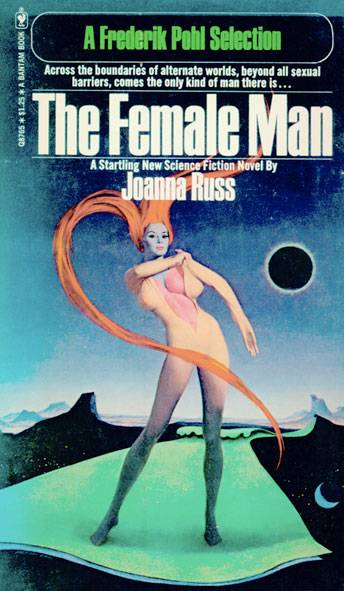
\includegraphics[width=0.5\paperwidth]{000000.jpg}
\end{figure}


\newpage
\vspace*{2\baselineskip}
\begin{center}
\textit{Książkę tę dedykuję Annie, Marii i~jeszcze jednej, oraz trzem
czwartym miliarda nas.}
\end{center}

\thispagestyle{empty}
\vspace*{7\baselineskip}

\begin{quotation}
Jeżeli Jackowi uda się coś zapomnieć, to mało przydatne jest, że Jill
mu o~tym ciągle przypomina. Jack musi skłonić ją, żeby tak nie robiła.
Najbezpieczniejszą metodą nie byłoby uciszenie jej, ale spowodowanie,
żeby i~ona również o~tym zapomniała.

Jack może wpływać na Jill na wiele sposobów. Może sprawić, że poczuje
się winna, że ciągle ,,przypomina''. Może deprecjonować jej doświadczenie.
Może zrealizować to mniej lub bardziej radykalnie. Jack może tylko
wykazać, że ta sprawa jest nieważna lub banalna, natomiast dla niej
jest ważna i~doniosła. Idąc dalej, Jack może zmienić modalność jej
doświadczeń, z~pamięci do wyobraźni: ,,Wyobrażasz to sobie tylko''.
Dalej, może unieważnić treść: ,,To nie było tak''. W~końcu, może zdeprecjonować
nie tylko ważność, modalność i~treść, ale także jej umiejętność pamiętania i~sprawić, że poczuje się winna za robienie tego w~ramach targowania.

To nie jest niezwykłe. Ludzie ciągle sobie robią takie rzeczy. Jednakże,
aby taka międzyosobowa deprecjacja zadziałała, warto pokryć ją grubą
warstwą mistyfikacji. Przykładowo, przez zaprzeczanie, że ta osoba
właśnie to robi, następnie przez podważanie takich spostrzeżeń, że
tak robi powiedzeniami takimi jak ,,Jak możesz myśleć takie rzeczy?''

,,Musisz być paranoikiem''. I~tak dalej.
\end{quotation}
\textit{R.D. Laing, The Politics of Experience, Penguin Books, Ltd., London,
1967, pp.31-32\footnote{tłumaczenie własne - przyp. tłum.}}


\part*{Część pierwsza}

\chapter{I}

Urodziłam się na farmie na Relaksowie\footnote{oryg. Whileaway zapewne od \textit{to be while away} tj.~\textit{spędzać czas bezczynnie, ale przyjemnie}, stąd Relaksowo -przyp.tłum.}. Kiedy miałam pięć lat, zostałam posłana do szkoły na Południowym Kontynencie (jak każda), a~kiedy skończyłam dwanaście lat, powróciłam do rodziny. Moja matka miała na imię Eva, moja druga matka - Alicia. Nazywam się Janet Evasyn. Kiedy miałam trzynaście lat, wytropiłam i~zabiłam wilka, sama z~karabinem, na Północnym Kontynencie, powyżej czterdziestego ósmego równoleżnika. Zrobiłam sanie na głowę i~łapy, potem porzuciłam głowę, a~w końcu wróciłam z~jednym pazurem, wystarczającym dowodem (jak myślałam). Pracowałam w~kopalniach, w~rozgłośni radiowej, na fermie mleka, plantacji warzyw, i~przez sześć tygodni jako bibliotekarka po złamaniu nogi. W wieku trzydziestu lat urodziłam Yuriko Janetsyn. Kiedy wyjeżdżała do szkoły pięć lat później (nigdy nie widziałam takiego sprzeciwu u dzieci), zdecydowałam się wziąć wolne i~sprawdzić, czy odnajdę swój stary rodzinny dom, choć matki wyprowadziły się stamtąd, gdy wzięłam ślub, i~przeniosły się do Mine City na Południowym Kontynencie. Miejsce było jednak nie do znalezienia. Nasze tereny wiejskie ciągle się zmieniają. Znalazłam tylko trójnogi radiolatarni komputerowych, dziwne rośliny, których wcześniej nie widziałam, na polach i~bandę wędrujących dzieci.

Kierowały się na Północ, by odwiedzić stację polarną i~zaoferowały
mi śpiwór, ale odmówiłam i~zostałam z~lokalną rodziną. Rano ruszyłam
do domu. Od tego czasu jestem Strażniczką Bezpieczeństwa w~hrabstwie,
to jest Bezpieczeństwo i~Pokój, stanowisko, które utrzymywałam
przez sześć lat. Mój skorygowany stanfordzki iloraz Bineta (w waszych
określeniach) wynosi 187, mojej żony 205, a~córki 193. Yuki jest świetna
w testach ustnych. Nadzorowałam kopanie szlaków przeciwpożarowych,
odbierałam porody, naprawiałam maszyny i~wydoiłam więcej muu-krów
niż chciałabym widzieć. Ale Yuki uwielbia lody. Kocham swoją córkę.
Kocham swoją rodzinę (jest nas dziewiętnaścioro) Kocham swoją żonę
(Vittorię). Miałam cztery pojedynki. Zabiłam cztery razy.

\chapter{II}

Jeannine Dadier\footnote{czyt. Dadjer} trzy razy w~tygodniu pracowała jako
bibliotekarka dla WPA\footnote{WPA - Works Progress Administration - amerykańska agencja okresu Nowego Ładu zatrudniająca miliony pracowników, powstała w~1935. Celem było zatrudnienie bezrobotnych w~okresie kryzysu 1929 roku. \url{https://en.wikipedia.org/wiki/Works_Progress_Administration} [dostęp 18-02-2021]- przyp.tłum.} w Nowym Jorku. Pracowała w~oddziale Tompkins Square Branch, w~części literatury dla młodzieży. Zastanawiała się czasami, czy śmierć Herr Shicklgrubera w~1936 była takim szczęściem (biblioteka miała książki na ten temat). W~trzeci poniedziałek marca 1969 roku zobaczyła pierwsze nagłówki o~Janet Evasyn, ale nie zwróciła uwagi. Cały dzień spędziła przybijając pieczątki w~książkach dla młodzieży i~sprawdzając w~małym lusterku zmarszczki wokół oczu (Mam tylko dwadzieścia dziewięć lat!). Dwa razy musiała podwinąć spódnicę nad kolana i~wspiąć się na drabinę po wyżej odłożone książki. Raz musiała przesunąć drabinę koło pani Allison i~nowego asystenta, którzy rozsądnie dyskutowali o~możliwości wojny z~Japonią. W~Saturday Evening Post był artykuł.

- Nie wierzę w~to - powiedziała miękko Jeannine Nandy Dadier. 

Pani Allison była Murzynką. To był niezwykle ciepły, mglisty dzień z~odrobiną
zieleni pokazującej się w~parku: fikcyjna zieleń, jak gdyby świat
zmienił kierunek i~zmierzał do wiosny w~niewyraźnych uliczkach, chmury
wyobraźni dookoła drzew.

- Nie wierzę w~to - powtórzyła Jeannine Dadier, nie wiedząc o~czym
rozmawiali. 

- Lepiej, żebyś uwierzyła! - powiedziała ostro pani Allison.

Jeannine balansowała na jednej nodze. (Dobre dziewczęta tak nie robią).
Zeszła z~drabiny z~książkami i~położyła je na stole dla rezerwacji.
Pani Allison nie lubiła dziewcząt z~WPA. Jeannine ponownie zobaczyła
nagłówki w~gazecie Pani Allison.

KOBIETA POJAWIŁA SIĘ ZNIKĄD NA BROADWAYU, POLICJANT ZAGINĄŁ 

- Nie wie\ldots (Mam kota, mam swój pokój, mam płytę grzejną, mam okno, mam
drzewo ajlanta).

Kątem oka zobaczyła Cala na ulicy. Szedł buńczucznie, kapelusz był
przechylony na czoło. Chciał coś powiedzieć głupiego o~byciu reporterem,
mała ostra twarz i~poważne niebieskie oczy. ,,Pewnego dnia mi się
uda, słonko.'' Jeannine wsunęła się pomiędzy regały, ukrywając się
za gazetą pani Allison: 

,,Na Broadwayu pojawiła się znikąd kobieta, policjant zaginął''. 

Marzyła o~owocach kupionych na rynku, choć jej
ręce pociły się, gdy kupowała poza rządowym sklepem i~nie umiała się
targować. Kupiłaby jedzenie dla kotów i~nakarmiłaby Pana Szronka zaraz
po wejściu do pokoju. Jadłby ze starego chińskiego talerzyka. Jeannine
wyobraziła sobie Pana Szronka ocierającego się o~jej nogi, falujący
ogon. Pan Szronek był czarno-biały. Z~zamkniętymi oczami, Jeannine
zobaczyła, jak wskakuje na półkę i~chodzi pomiędzy jej rzeczami, jej
muszlami i~miniaturkami. ,,Nie, nie, nie!'' powiedziała. Kot zeskoczył,
strącają jedną z~jej japońskich lalek.

Po obiedzie, Jeannine wyprowadziłaby go. Potem pozmywała naczynia
i próbowała naprawić jej stare ubrania. Przejrzałaby książeczkę z
kartkami na żywność. Gdy zrobiłoby się ciemno, włączyłaby radio na
wieczorną audycję, lub poczytałaby, może zadzwoniła z~apteki i~zapytała
się o~ten pensjonat w~New Jersey. Mogłaby nawet zadzwonić do brata.
Na pewno zasadziłaby nasiona pomarańczy i~je podlała. Pomyślała o
Panu Szronku skradającym się pomiędzy miniaturowymi drzewkami pomarańczowymi,
wyglądałby jak tygrys. Gdyby dostała puste puszki w~rządowym sklepie.

- Cześć mała? - To był wstrętny szok. To Cal.

- Nie - powiedziała szybko Jeannine. - Nie mam czasu.

- Kochanie? - ciągnął ją za ramię. - Chodź na kawę. - Ale nie mogła. Musiała
uczyć się greki (taka książka była na stole dla rezerwacji). Było
tak wiele do zrobienia.

Cal marszczył brwi i~błagał. Czuła poduszkę pod plecami, a~Pan Szronek
chodził dookoła nich, patrząc na nią swoimi dziwnymi błękitnymi oczami,
krocząc wściekle dookoła kochanków. Częściowo syjamczyk, Cal nazywał
go ,,Poplamionym Chudym Kotem''. Cal ciągle chciał eksperymentować na
nim, upuszczał go z~krzesła, kładł rzeczy na jego drodze, chował je
przed nim. Pan Szronek teraz tylko prychał na niego.

- Później - powiedziała zdesperowana Jeannine. Cal pochylił się i
wyszeptał do jej ucha. Zachciało jej się płakać. Cal zabujał się na
stopach. Potem powiedział: 

- Poczekam 

Usiadł na krześle Jeannine,
wziął do ręki gazetę i~dodał: 

- Znikająca kobieta. To Ty. 

Jeannine zamknęła oczy i~zaczęła marzyć o~Panu Szronku, zwiniętym na kominku, spokojnie śpiącym, cała kotowatość
w kręgu.

Co za zepsuty kotek.

- Kochanie? - powiedział Cal.

- Och, dobrze - powiedziała zdesperowana Jeannine - już dobrze.

Popatrzę na kwiatek.

\chapter{III}

Janet Evason pojawiła się na Broadwayu o~drugiej popołudniu w~bieliźnie.
Nie straciła głowy. Chociaż ciało chciało podtrzymać poprzedni ruch,
Janet, sekundę po przybyciu, przyjęła pozycję obronną (bardzo dobrze)
z rozwianymi włosami, w~szortach khaki i~koszuli poplamionej potem.
Kiedy policjant próbował chwycić ją za ramię, zagroziła mu ciosem
savate, ale znikł. Janet z~przerażeniem patrzyła na tłum dookoła niej.
Policjant pojawił się w~tym samym miejscu godzinę później, nie pamiętając
nic z~tej przerwy, ale Janet Evasyn wróciła do swojego śpiwora w~Nowym
Lesie już po kilku chwilach. Kilka słów w~wszechruskim i~już jej nie
było. Ostatnie z~nich obudziły osobę obok w~Nowym Lesie.

- Idź spać - powiedział anonimowy ,,przyjaciel na noc'', nos, czoło i
lok czarnych włosów nakrapianych światłem księżyca.

- Ale kto paprał mi w~głowie! - odpowiedziała Janet Evasyn.

\chapter{IV}

Kiedy Janet Evason wróciła do Nowego Lasu, a~eksperymentatorzy w~Stacji
Polarnej zaśmiewali się (bo to nie był sen), byłam na koktajlu na
Manhattan. Właśnie zmieniłam się w~mężczyznę, ja, Joanna. Znaczy mężczyznę
rodzaju żeńskiego, oczywiście. Moje ciało i~dusza były identyczne.

Zatem ja również.

\chapter{V}

Pierwszy mężczyzna, który postawił stopę w~Relaksowie, pojawił się
na polu rzepy na Północnym Kontynencie. Był ubrany na niebiesko, jak
turysta, z~niebieską czapką. Ludzie na farmie zostali zawiadomieni.
Jeden, widząc punkcik na skanerze podczerwieni traktora, podleciał,
żeby go zabrać. Mężczyzna w~niebieskim zobaczył maszynę latającą bez
skrzydeł, ale podnoszącą kurz. Warsztat naprawczy dla maszyn farmerskich
w tym tygodniu był niedaleko, więc kierowca traktora tam go zaprowadził.
Mężczyzna nie mówił nic zrozumiałego. Zobaczył przezroczystą kopułę,
powierzchnia delikatnie falowała. Z~jednej strony był wylot wentylatora.
Pod kopułą była dżungla maszyn, martwe, na boku, niektóre otwarte,
ich wnętrzności wypływające na trawę. z~szerokiej ramy pod dachem machały
ręce wielkie jak trzech mężczyzn. Jedna z~nich podniosła samochód
i upuściła go. Boki samochodu odpadły. Mniejsze dłonie wyskoczyły
z trawy.

- Hej, hej! - krzyknął kierowca traktora, uderzając kawałem żelaza
w ścianę. - Upadło, zemdlało!

- Wyślij to z~powrotem - powiedział operator, wychodząc spod hełmu
indukcyjnego po drugiej stronie warsztatu. Czworo innych wyszło i
stanęło dookoła mężczyzny w~niebieskim garniturze.

- Czy jest stabilny? - powiedziało jedno.

- Nie wiemy.

- Czy jest chory?

- Zahipnotyzuj go i~wyślij go z~powrotem.

Mężczyzna w~niebieskim, gdyby to zobaczył, byłby nimi zdziwiony, gładkie
twarze, gładka skóra, zbyt niskie, zbyt pulchne, ich kombinezony szerokie
w biodrach. Nosili kombinezony, ponieważ nie wszystko można było naprawić
mechanicznymi dłońmi, czasem trzeba było swoich własnych. Jeden były
stary i~miał białe włosy, inny był bardzo młody, jeden nosił długie
włosy czasem doceniane przez młodych Relaksowa, ,,by miło spędzić
czas''. Sześć par zaciekawionych oczu przyglądało się mężczyźnie w
niebieskim garniturze.

- To, mes enfants, - powiedział w~końcu kierowca traktora - jest mężczyzna. To prawdziwy mężczyzna z~Ziemi.

\chapter{VI}

Czasem pochylasz się, żeby zawiązać sznurowadło i~wtedy, albo je wiążesz,
albo nie. Albo natychmiast się prostujesz, albo nie. Każdy wybór tworzy
co najmniej dwa światy możliwe, to jest, jeden w~którym coś zrobiłaś
i drugi, w~którym czegoś nie zrobiłaś. Lub prawdopodobnie o~wiele
więcej: jeden, gdzie robisz szybko, ten, w~którym robisz wolno, jeden,
gdzie nie robisz, ale się wahasz, jeden, w~którym się wahasz marszcząc
brwi, inny w~którym się wahasz kichając, i~tak dalej. Idąc dalej,
musi istnieć nieskończona liczba możliwych wszechświatów (tak płodny
jest bóg), ponieważ nie ma powodu, by wyobrażać sobie Natury jako
uprzedzonej tylko do ludzkiej działalności. Każde przesunięcie dowolnej
cząsteczki, każda zmiana orbity dowolnego elektronu, każdy kwant światła,
który wpada tutaj, a~nie tam, wszystko to musi mieć gdzieś swoją alternatywę.

Jest również możliwe, że nie istnieje jedna prosta linia, czy pasmo
prawdopodobieństwa, że żyjemy raczej w~ich skręconym splocie, niezauważalnie
rozmywające przejście z~jednego do drugiego, póki nie przekroczymy
granic zbioru zmiennych, które właściwie nie mają dla nas znaczenia.
Zatem paradoks podróży w~czasie przestaje działać, ponieważ przeszłość,
którą ktoś odwiedza, nie jest kogoś przeszłością, ale już innej osoby,
lub inaczej, podróż kogoś do przeszłości natychmiast tworzy inną teraźniejszość
(taką w~której podróż się odbyła) i~to, co odwiedzasz jest przeszłością
należącą do tej teraźniejszości, całkowicie odmienną od Twojej własnej
przeszłości. A~z~każdą decyzją (w tej nowej przeszłości) rozgałęzia
się nowy prawdopodobny wszechświat, tworząc jednocześnie nową przeszłość
i nową teraźniejszość, lub, dla uproszczenia, nowy wszechświat. I
kiedy wracasz do swojej własnej teraźniejszości, tylko Ty wiesz, jaka
była poprzednia przeszłość i~co w~niej zrobiłaś.

A zatem jest prawdopodobnie, że Relaksowo, nazwa Ziemi za dziesięć
wieków, ale nie naszej Ziemi, jeżeli mnie rozumiesz, w~ogóle nie będzie
pod wpływem wydarzeń w~przeszłości kogoś innego. I, oczywiście, na
odwrót. Te dwa równie dobrze mogą być niezależnymi światami.

Relaksowo, jak już rozumiesz, jest w~przyszłości.

Ale nie naszej przyszłości.

\chapter{VII}

Zobaczyłam Jeannine nieco później, w~barze, gdzie poszłam zobaczyć
Janet Evasyn w~telewizji (nie miałam własnego telewizora). Jeannine
wyglądała bardzo nie na miejscu. Usiadłam obok niej, a~ona mi się
zwierzyła: 

- Nie pasuję tutaj. 

Nie wiem, jak się tutaj znalazła, za
wyjątkiem przypadku. Wyglądała, jak gdyby ubrała się na plan filmowy,
siedząc w~cieniu, z~tą jej chustką na głowie, jeansach, długonoga,
trzpiotowata dziewczyna w~ubraniach trochę dla niej za małych.

Moda (zdaje się) po Wielkiej Depresji powoli ożywa. Nie tutaj i~teraz,
oczywiście. 

- Nie pasuję tutaj! - wyszeptała znowu przestraszona Jeannine
Dadier. Wierciła się. 

- Nie lubię takich miejsc. - powiedziała.

Dźgnęła czerwone skórzane obicie fotela. 

- Co? - spytałam.

- Wędrowałam pieszo na urlopie - powiedziała poważnie. - Lubię to.
To zdrowe.

Wiem, że zdrowe bieganie po łąkach jest prawdopodobnie cnotliwe, ale
lubię bary, hotele, klimatyzację, dobre restauracje i~odrzutowce,
i powiedziałam jej o~tym.

- Odrzutowce? - spytała.

Janet Evasyn pojawiła się w~telewizorze. Było to tylko zdjęcie. Potem
były wiadomości z~Kambodży, Laosu, Stanu Michigan, Jeziora Canadaigua
(zanieczyszczenie) i~obracający się globus w~kolorze z~siedemnastoma
sztucznymi satelitami latającymi naokoło. Kolory były okropne. Byłam
kiedyś w~studio telewizyjnym, balkon biegnący naokoło ścian stodoły,
każdy centymetr dachu zajęty przez reflektory, po to by drobna kobieta
z delikatnym głosem mogła się dąsać nad piekarnikiem lub zlewem. Wtedy
pojawiła się Janet Evasyn wyglądając blado jak wszyscy ludzie w~telewizji.
Poruszała się ostrożnie i~rozglądała się z~zainteresowaniem. Dobrze
się ubrała (garnitur). Gospodarz, czy mistrz ceremonii, czy jak się
tam nazywa, uścisnął jej dłoń i~potem wszyscy podali sobie ręce, jak
na weselu francuskim, albo we wczesnym niemym filmie. Gospodarz był
ubrany w~garnitur. Ktoś poprowadził ją do fotelu, a~ona uśmiechnęła
się i~kiwnęła głową w~przesadny sposób, jak wtedy, gdy nie wiesz,
czy robisz coś dobrze. Janet rozejrzała się i~osłoniła oczy przed
światłem. Potem przemówiła.

(Pierwszą rzeczą, jaką powiedział drugi mężczyzna, który kiedykolwiek
odwiedził Relaksowo było: ,,Gdzie są wszyscy mężczyźni?''. Janet Evasyn,
gdy pojawiła się w~Pentagonie, ręce w~kieszeniach, stopy rozstawione
szeroko, powiedziała: ,,Gdzie cholercia są wszystkie kobiety?'').

Dźwięk w~telewizorze na moment znikł i~Jeannine Dadier znikła. Nie
zniknęła, po prostu już tutaj nie była. Janet Evasyn wstała, potrząsnęła
znowu rękami, rozejrzała się, spojrzała się z~powątpiewaniem, udała
zrozumienie, kiwnęła głową i~wyszła poza zasięg kamer. Nigdy nie pokazywali
strażników.

Wysłuchałam jej następnym razem i~szło to tak: 

\textsc{Gospodarz}: Jak się Pani tu podoba, panno Evasyn?

\textsc{Janet} (rozglądając się po studio, zmieszana): Jest za gorąco.

G: Mam na myśli, jak się tutaj Pani podoba, na Ziemi?

J: Ale ja żyję na ziemi. (Jej uwaga była trochę napięta).

G: Może mogłaby Pani wytłumaczyć, co Pani ma na myśli, to znaczy istnienie
różnych prawdopodobieństw i~tak dalej, mówiła Pani o~tym wcześniej.

J: To jest w~gazetach.

G: Ale panno Evasyn, jeżeli mogłaby Pani wytłumaczyć to tym, którzy
oglądają ten program.

J: Niech przeczytają. Nie umieją czytać?

(Przez chwilę było cicho. Potem gospodarz programu przemówił.)

G: Nasi socjolodzy oraz fizycy twierdzą, że będą musieli zrewidować
wiele teorii w~świetle informacji przedstawionych przez naszego gościa
z innego świata. Na Relaksowie nie było ludzi przez ostatnie osiem
wieków, znaczy nie mam na myśli ludzi, oczywiście, ale mężczyzn, i
to społeczeństwo, kierowane całkowicie przez kobiety, ściągnęło na
siebie bardzo dużo uwagi od chwili pojawienia się w~zeszłym tygodniu
jego reprezentanta i~pierwszego ambasadora, damy po mojej lewej stronie.
Janet Evasyn, czy mogłaby Pani powiedzieć nam, jak według Pani społeczeństwo
Relaksowa zareaguje na pojawienie się mężczyzn z~Ziemi, mam na myśli
naszą teraźniejszą Ziemię, oczywiście, po osiemsetletniej izolacji?

J: (podskoczyła na to pytanie, prawdopodobnie dlatego, że było to
pierwsze pytanie, które zrozumiała) Dziewięćset lat. Jakich mężczyzn?

G: Jakich mężczyzn? Z~pewnością oczekujecie odwiedzin mężczyzn naszego
społeczeństwa.

J: Dlaczego?

G: Dla wiedzy, handlu, hm, kontaktów kulturalnych. (śmiech) Wydaje
mi się, że mi Pani to utrudnia, panno Evasyn. Gdy Zaraza, o~której
Pani mówiła, zabiła mężczyzn na Relaksowie, czy ich nie brakowało?
Czy rodziny nie rozpadły się? Czy nie zmienił się styl życia?

J (powoli): Przypuszczam, że ludziom zawsze brakuje tego, do czego
byli przyzwyczajeni. Tak, brakowało ich. Nawet zbioru słów, jak ,,on'', ,,mężczyzna'' i~tak dalej, te słowa są zakazane.

Potem drugie pokolenie, używa ich, by pokazać odwagę, pomiędzy sobą,
a trzecia generacja nie używa, by pokazać wychowanie, a~przy czwartej,
kogo to obchodzi? Kto pamięta?

G: Ale z~pewnością, to jest\ldots

J: Przepraszam, może błędnie rozumiem, co chcesz powiedzieć, bo język,
w którym mówimy, jest tylko moim hobby, nie mówię tak płynnie, jak
bym chciała. My mówimy wszechruskim, którego nawet Rosjanie by nie
zrozumieli. to jak średniowieczna angielszczyzna dla Was, tylko na
odwrót.

G: Rozumiem. Ale wracając do mojego pytania, 

J: Tak.

G: (Trudna sytuacja, pomiędzy władzami a~tą dziwną osobą, która jest
nieświadoma jak wódz dzikusów, bez wyrazu, uprzejmy, pewnie cywilizowany,
całkowicie nierozumiejący. W~końcu mówi): Czy nie chcecie powrotu
mężczyzna na Relaksowo, panno Evasyn?

J: Dlaczego?

G: Jedna płeć to połowa gatunku, panno Evasyn. Cytuję tu (i zacytował
znanego antropologa). Czy chcecie wygnać seks z~Relaksowa?

J (z solidną godnością i~kompletną naturalnością): Hm?

G: Spytałem, czy chcecie wypędzić seks z~Relaksowa? Seks, rodzina,
miłość, przyciąganie erotyczne, proszę nazwać, jak Pani chce, wiemy,
że jesteście kompetentnymi i~inteligentnymi jednostkami, ale czy sądzi
Pani, że to wystarczy? Na pewno wie Pani o~biologii innych gatunków,
by rozumieć o~czym mówię.

J: Jestem żonata. Mam dwoje dzieci. O~czym, do diabła, pan mówi?

G: Ja, panno Evason, my, cóż, wiemy, że tworzycie to, co nazywacie
małżeństwami, panno Evasyn, że uznajecie pochodzenie dzieci od obojga
partnerów i~że nawet macie ,,plemiona'', nazywam je tak według tego
jak nazywa je profesor \_\_\_\_\_\_\_\_\_\_\_. Wiem, że tłumaczenie
nie jest doskonałe. Wiemy, że te małżeństwa lub plemiona tworzą świetne
instytucje wsparcia ekonomicznego dla dzieci i~dla swego rodzaju mieszania
genów, choć, muszę wyznać, wyprzedzacie nas w~sferze biologii. Ale,
panno Evasyn, nie mówię tu o~relacjach ekonomicznych, ani nawet o
emocjonalnych. Oczywiście matki Relaksowa kochają swoje dzieci, nikt
w to nie wątpi. I~oczywiście, kochają się wzajemnie, w~to także nikt
nie wątpi. Ale jest przecież więcej, znacznie, znacznie więcej, mam
na myśli miłość seksualną.

J (ze zrozumieniem): Och! Chodzi o~kopulację.

G: Tak.

J: I~mówicie, że tego nie znamy?

G: Tak.

J: Jakie to głupie. Oczywiście, znamy.

G: Ach? (Chce powiedzieć, ,,Proszę mi nie mówić.'')

J: Ze sobą. Pozwól, że wytłumaczę.

Janet została natychmiast zastąpiona przez reklamę poetycko opisującą
radości niekrojonego chleba. Wzdrygnęli się (poza zasięgiem kamery).
Nie doszłoby do tego, gdyby Janet nie naciskała na dołączenie systemu
,,nie-dotykaj-mnie'' do systemu odtwarzania nagrania. To była transmisja
na żywo opóźniona o~cztery sekundy. Zaczynałam ją coraz bardziej lubić.
Powiedziała: 

- Jeżeli oczekujecie, że będę przestrzegać waszych tabu,
myślę, że powinniście być precyzyjniejsi w~ich określeniu. 

W~świecie
Jeannine Dadier, żeński prowadzący zapytał (zapytałaby): 

- W~jaki sposób kobiety Relaksowa układają włosy?

J: Przycinają je przy pomocy muszli.

\chapter{VIII}

- Ludzkość jest nienaturalna! - zawołała filozofka Dunyasha Bernadettesyn
(P.K.~344-426), która przez całe życie cierpiała z~powodu błędu genetyka,
który dał jej żuchwę jednej matki i~zęby drugiej matki. Ortodoncja
jest rzadko potrzebna na Relaksowie. Niemniej jednak, zęby jej córki
były doskonałe.

Zaraza pojawiła się na Relaksowie w~17 roku P.Z. (Przed Zarazą) i
zakończyła się w~P.K.~3 (Po Katastrofie), połowa populacji martwa. Rozpoczęła się tak wolno, że nikt o~niej nie wiedział, póki nie było za późno. Zaraza dotykała tylko mężczyzn.
Ziemia była kompletnie odbudowana w~trakcie Złotego Wieku (P.Z. 300
- ok. P.Z. 180). Środowisko naturalne powodowało znacząco mniejsze
problemy, niż mogłoby, gdyby podobna katastrofa przydarzyła się wieki
wcześniej. W~czasach Rozpaczy (jak potocznie nazywano ten okres),
Relaksowo składało się z~dwóch kontynentów, nazwanych po prostu Północnym
i Południowym Kontynentem, a~w linii brzegowej znajdowało się wiele
idealnych zatoczek i~kotwicowisk.

Ciężkie warunki klimatyczne nie docierały poniżej równoleżników: 72
stopnie południowy i~68 stopni północny. Konwencjonalny ruch wodny,
w czasach Katastrofy, był wykorzystywany prawie tylko do transportu,
ruch pasażerski używał mniejszych poduszkowców na elastycznie dopasowanych
trasach. Domy były samowystarczalne, z~przenośnymi źródłami energii,
silnikami alkoholowymi lub panelami słonecznymi, zastępującymi wcześniejsze
scentralizowaną energetykę. Późniejszy wynalazek praktycznych reaktorów
antymaterii (K. Ansky, P.K. 239) zaowocował wielkim optymizmem na jakąś
dekadę, ale te urządzenia były zbyt nieporęczne do wykorzystania w
domu. Katharina Lucysyn Ansky (P.K. 201-282) była również odpowiedzialna
za zasady, który umożliwiły chirurgię genetyczną. (Łączenie jajeczek
było znane przez poprzednie półtora wieku). Populacja zwierząt stała
się tak deficytowa przed Złotym Wiekiem, że wiele gatunków zostało
przywróconych przez entuzjastów w~okresie Ansky. W~280 P.K. zanotowano
wybuch populacji królików w~Newland (wyspie na krańcu Północnego Kontynentu),
pandemię nie bez historycznego poprzednika. Do 492 P.K., dzięki błyskotliwej
agitacji wspaniałej Betty Bettinasyn Murano (P.K 453-P.K.502), kolonie
ziemskie zostały odbudowane na Marsie, Ganimedesie i~na asteroidach,
przy pomocy Ligi Księżycowej, zgodnie z~traktatem Mare Tenebrum (P.K.
240). Zapytana, czego spodziewa się znaleźć w~kosmosie, Betty Muran
odpowiedziała nieśmiertelnym żartem: ,,Nic''. W~trzecim wieku Po Katastrofie
inteligencja była kontrolowanym i~dziedzicznym czynnikiem, choć umiejętności
i zainteresowania nadal umykały chirurgom, a~tylko całkowita inteligencja
mogła być podniesiona. W~piątym wieku, organizacja klanowa osiągnęła
obecny złożony stan i~odzyskiwanie fosforu było prawie kompletne.
Do siódmego wieku, kopalnie Jowisza umożliwiły zastąpienie technologii
szkła i~ceramiki metalami (które również były ponownie wykorzystywane)
i~po raz trzeci w~ciągu czterystu lat (również mody są czasami cykliczne)
pojedynkowanie się stało się poważnym problemem społecznym. Wiele
lokalnych Rad Gildii przegłosowało, że zwyciężczyni w~pojedynku musi
ponieść karę za przypadkowe morderstwo i~urodzić dziecko w~zamian
za utracone życie, ale rozwiązanie było zbyt proste, by stać się popularnym.
Przykładowo, problemem mógł być wiek obu uczestniczek pojedynku. Na
początku dziewiątego wieku P.K. hełmy indukcyjne stały się powszechne,
przemysł został drastycznie zmieniony, a~Liga Księżycowa w~końcu przewyższyła
Południowy Kontynent w~produkcji białka na osobę rocznie. W~913 P.K.
mroczna i~niezadowolona następczyni Katy Ansky zebrała różne elementy
wiedzy matematycznej i~odkryła, lub wynalazła, mechanikę rachunku
prawdopodobieństwa.

W czasach Jezusa z~Nazaretu, droga czytelniczko, nie było samochodów.
Ciągle jednak czasem spaceruję.

Oznacza to, że rozważna ekolożka projektuje rzeczy, aby pracowały
tak doskonale, jak można, ale na wszelki wypadek dobrze jest mieć
lampę naftową w~stodole, a~dyskusja o~utrzymaniu koni zwykle kończy
się decyzją, że to zbyt wiele kłopotu, więc puszcza się konie wolno.
Niemniej rezerwat w~La Jolla nadal opiekuje się końmi. Nie rozpoznałybyśmy
ich. Hełm indukcyjny umożliwia jednej robotnicy nie tylko mieć siłę,
ale także płynność i~kontrolę tysięcy. Wywróciło to przemysł Relaksowa
do góry nogami. Większość ludzi chodzi na Relaksowie (oczywiście,
ich stopy są doskonałe). Czasem dziwacznie się śpieszą. We wczesnym
okresie, wystarczyło utrzymać się przy życiu i~rodzić dzieci. Teraz
mówią, że ,,kiedy re-industrializacja się skończy'' i~nadal chodzą.
Może to lubią.

Mechanika probabilistyczna oferuje możliwość teleportacji poprzez
zapętlenie do innego, precyzyjnie wybranego kontinuum. Chilia Ysayesyn
Belin żyje we włoskich ruinach (myślę, że to część posągu Vittore
Emmanuele, jednak nie wiem, jak się dostał do Newland) i~jest do niego
przywiązana. Jak można by dyskretnie dodać instalację wodociągową bez
nadmiernego nakładu pracy? Jej matka, Ysaye, żyje w~jaskini (ta Ysaye,
która stworzyła teorię mechaniki probabilistycznej).

Prefabrykaty można dostać w~dwa dni i~od razu je składać. Belinów
jest osiemnaścioro, i~dwadzieścia trzy Moujki (rodzina Ysaye, mieszkałam
u obojga).

Relaksowo nie ma prawdziwych miast. I, oczywiście, kultura na prowincji
jest kilka wieków za centrum. Relaksowo jest tak wiejskie, że czasami
zastanawiam się, czy najwyższe wyrafinowanie nie zabierze nas do rodzaju
wieku przed erą kamienną, ogrodu bez artefaktów, prócz tych, które
będziemy nazywać cudami. Moujki wynalazła w~czasie wolnym w~904 P.K.
pojemniki na żywność wielorazowego użytku, ponieważ idea ją fascynowała.
Ludzie byli zabijani za mniej.

W międzyczasie, ekologiczne sprzątanie jest ogromne.

\chapter{IX}

JE: Urodziłam moje dziecko w~wieku trzydziestu lat, wszystkie tak
robimy. To wakacje. Prawie pięć lat.

Pokoje dzieci pełne są ludzi czytających, malujących, śpiewających,
ile tylko mogą, dzieciom, z~dziećmi, nad dziećmi. Jak w~starym chińskim
zwyczaju trzyletniej żałoby, przerwa we właściwym czasie.

Przedtem nie ma odpoczynku i~będzie tak mało potem\ldots wszystko, co
robię, rozumiesz, mam na myśli, naprawdę robię, muszę zawrzeć dokładnie
w tych pięciu latach. Każdy pracuje w~chorym pośpiechu. Przy sześćdziesiątce
dostanę siedzącą pracę i~znów będę miała trochę czasu dla siebie.

\textsc{Prowadzący}: I~to jest postrzegane za wystarczające, na Relaksowie?

JE: Mój Boże, nie.

\chapter{X}

Jeannine się guzdrze. Zawsze nienawidziła wstawania z~łóżka. Chciałaby
leżeć na boku i~patrzyć na ajlanta, póki nie zaczęłyby ją boleć plecy.
Wtedy by się przełożyła na drugi bok, ukryta za liśćmi i~zasnęła.
Dokończyć sny, póki leży w~łóżku z~mętlikiem, a~kot mógłby się na
niej położyć. W~dni pracujące, Jeannine wstaje wcześnie w~rodzaju
koszmaru na jawie: czuje się okropnie, potyka się w~drodze do łazienki
cała zaspana. Kawa ją mdli. Nie może usiąść w~fotelu, założyć kapci,
pochylić, oprzeć się, lub położyć. Pan Szronek, przechadzając się po parapecie, kroczy tam i~z powrotem przed ailantem, tygrys w~dżungli. Muzeum. Zoo. Autobus do Chinatown.

Jeannine zatopiła się w~drzewie z~wdzięcznością, jak syrena, z~herbatą
w ręku, przyjemnie dać młodemu mężczyźnie, który miał wielką muffinkę
drżącą nad obrożą zamiast twarzy, która tam powinna być. Drżącą z
emocji.

Kot przemówił. Wzdrygnęła się. 

Zaraz Cię nakarmię, Panie Szronku.

Mrrrr.

Cala nie stać na to, aby mnie gdzieś zabrać. Podróżowała tak długo
publicznymi autobusami, że zna wszystkie trasy. Strasznie ziewając,
zalała wodą jedzenie Pana Szronka i~postawiła talerzyk na podłodze.
Jadł dystyngowanie. Przypomniała sobie, jak zabrała go do jej brata,
dali mu prawdziwą surową rybę, dopiero co złapaną w~stawie przez jednego
z chłopców i~jak Pan Szronek rzucił się na rybę, błyskawicznie, taki
był żarłoczny. One naprawdę lubią ryby. Teraz kotek bawi się talerzykiem,
uderzając go z~miejsca na miejsca, choć już był dorosły. Koty naprawdę
były szczęśliwszy, gdy\ldots gdy\ldots (ziewnęła) Och, to było Chińskie
Święto.

Gdybym miała pieniądze, gdybym mogła pójść do fryzjera\ldots Wchodzi
do biblioteki, jest profesorem, nie, jest super przystojny. 

- Kim jest ta dziewczyna? - mówi do pani Allison, figlarnie jej pochlebiając. 

- To Jeannine - spuszcza oczy,
pełna kobiecego seksapilu. 

Muszę dziś zrobić paznokcie. I~te piękne
ubrania, są eleganckie, podkreślają moją osobowość, moje piękno. 

- Coś w~niej jest - mówi. - Pójdziemy gdzieś? 

Potem w~ogrodzie na dachu, pijąc szampana, 

- Jeannine, czy\ldots

Pan Szronek, niezadowolony i~zazdrosny, drapie ją w~nogę. 

- Dobrze!! - mówi, zachłystując się dźwiękiem swojego głosu. Ubiera się szybko.

Naprawdę (pomyślała Jeannine, patrząc na drogie duże lustro, w~niejasny
sposób zostawione przez poprzedniego najemcę w~drzwiach szafy) naprawdę
wyglądam trochę jak\ldots, jak tak nachylę twarz. Och! Cal będzie WŚCIEKŁY,
i biegnie do łóżka, zdejmuje piżamę i~łapie bieliznę, którą zawsze
wieczorem zostawia na biurku. Jeannine Nimfa Wodna. Marzyłam kiedyś
o młodym mężczyźnie. Do końca nie wierzy w~karty i~omeny, to całkiem
głupie, ale czasem chichocze i~myśli, że byłoby to miłe. Mam duże
oczy.

Spotkasz wysokiego, ciemnego, kładąc Pana Szronka delikatnie na łóżku,
wkłada sweter i~spódnicę, potem czesze włosy, licząc pociągnięcia
pod nosem. Jej płaszcz jest tak stary. Jeszcze trochę makijażu, szminka
i puder. (Znowu zapomniała i~puder jest na płaszczu). Jeżeli wstałaby
wcześniej, nie spotkałaby Cala, pobawiłby się z~kotem (na kolanach),
a potem chciałby się Kochać, tak jest lepiej. Autobus do Chinatown.
Potknęła się na schodach w~pośpiechu, chwytając się poręczy.

Drobna panna Spry, starsza pani na parterze, otworzyła drzwi dokładnie
w tym momencie, by zauważyć pannę Dadier biegnącą przez hol. Jeannine
ujrzała drobną, pomarszczoną, zmęczoną, starą twarz, delikatny białe
włosy, ciało jak worek mąki ubrany w~czarną bezkształtną suknię. Zauważyła,
pożyłkowana dłoń na framudze drzwi.

- Czyż, Jeannine, wychodzisz?

Przyśpieszając histerycznie, panna Dadier ucieka. Oooch! Żeby tak
wyglądać!

Cal właśnie mijał przystanek.

\chapter{XI}

Etsuko Belin, rozciągnięta krzyżem na szybowcu, przesunęła swój środek
ciężkości i~rozpoczęła wolny zwrot, obserwując pięćset metrów poniżej
wschód słońca Relaksowa odbijający się w~jeziorach polodowcowych Mount
Strom. Odwróciła szybowiec do góry nogami i~lecąc na plecach, minęła
jastrzębia.

\chapter{XII}

Sześć miesięcy temu w~Chiński Nowy Rok, Jeannine stała na zimnie,
trzymając rękawiczki przy uszach, aby ochronić się przed okropnym
dźwiękiem sztucznych ogni. Cal, obok niej, obserwował taniec smoka
na ulicach. 

\chapter{XIII}

Poznałam Janet Evasyn na Broadwayu, stojąc z~boku parady na jej cześć
(byłam). Wychyliła się z~limuzyny i~mnie przywołała. Otoczona przez
agentów Secret Service. 

- To ta - powiedziała. 

W~końcu wszystkie się spotkamy.

\chapter{XIV}

Jeannine, wyrwana z~miejsca, na farmie w~Relaksowie, zasłania uszy
i zaciska oczy, siedząc na koźle, pod drzwiami, gdzie wszyscy jedzą.
Nie ma mnie tu. Nie ma mnie tu. Najmłodszej córce Chilii Ysayesyn
spodobała się ta nowa. Jeannine widzi duże oczy, duże piersi, mocne
ramiona, grube usta, całe to obrzydlistwo. Pan Szronek jest rozpieszczany,
głaskany i~karmiony przez osiemnaście dziewczyn Beliny. Nie ma mnie
tu.

\chapter{XV}

\textsc{Janet}: W~Evasyn to nie syn, a~,,córka''. To wasze tłumaczenie.

\chapter{XVI}

I oto jesteśmy.

\part*{Część druga}

\chapter{I}

Kim jestem?

Wiem, kim jestem, ale jaka jest moja nazwa handlowa?

Ja z~nową twarzą, obrzękłą maską. Odłożona do starych, w~strzępach
plastyku, blond wampir na Halloween na mundurze SS. Byłam pod tym chuda
jak tyczka, prócz rąk, które były podobnie chude, i~ta imponująca
twarz. Zrobiłam tak w~biznesie, o~którym zaraz, i~przestraszyłam idealizujące
dzieci, które mieszkały piętro niżej. Ich delikatna skóra czerwona
ze strachu. Ich czyste, młode głosy śpiewające piosenkę (o~trzeciej
nad ranem). Nie jestem Jeannine. Nie jestem Janet. Nie jestem Joanną.

Nie robię tego często (to mówię ja, upiór), ale to świetna technika
w windzie, przycisnąć palec wskazujący do karku kogoś, mijając czwarte
piętro, wiedząc, że nigdy się nie dowie, że Cię tutaj nie ma.

(Przepraszam, ale uważaj).

Poznacie mnie później.

\chapter{II}

Tak jak mówiłam wcześniej, ja (ale nie ta powyżej, proszę) przeżyłam
doświadczenie siódmego lutego tysiąc dziewięćset sześćdziesiątego
dziewiątego.

Zmieniłam się w~mężczyznę.

Byłam już kiedyś mężczyzną, ale tylko krótko i~tylko w~tłumie.

Nie zauważyłybyście niczego, gdybyście tam były.

Męskość, dzieci, nie jest wynikiem odwagi czy krótkich włosów czy
nieczułości, czy pobytu (w moim przypadku) w~jedynym hotelu, w~wieżowcu
w Chicago, gdy na zewnątrz panoszy się śnieżyca. Siedziałam na przyjęciu
koktajlowym w~Los Angeles, wśród brzydkich barokowych mebli, zmieniona
w mężczyznę. Ujrzałam się pomiędzy zwojami lustra i~wyniki były niezaprzeczalne:
byłam mężczyzną. Ale czym zatem jest męskość?

Męskość, dzieci\ldots to męskość.

\chapter{III}

Janet zaprosiła mnie do limuzyny i~wsiadłam. Na drodze było bardzo
ciemno. Gdy otworzyła drzwi, zobaczyłam jej sławną twarz okoloną światłami
z przednich miejsc. Drzewa gromadziły elektryczną zieleń poza światłami
samochodu. Właśnie tak ją poznałam. Jeannine Dadier była nieuchwytnym
zarysem na tylnym siedzeniu.

- Pozdrowienia - powiedziała Janet Evasyn. - Cześć. Bonsoir. To jest
Jeannine. A~Ty?

Powiedziałam jej. Jeannine zaczęła opowiadać o~wszystkich mądrych
rzeczach, które zrobił jej kot. Drzewa kołysały się i~szarpały przed
nami.

- W~księżycowe noce - powiedziała Janet - często jadę bez świateł.
- I~zwalniając samochód, wyłączyła światła. Znaczy, zobaczyłam, jak
znikają, krajobraz mieszaniny mgły i~bladości aż do horyzontu, jak
źle oświetlony Watteau. Zawsze w~świetle księżyca odnoszę wrażenie,
jak gdyby wzrok mi się pogorszył. Samochód, coś drogiego, choć było
zbyt ciemno, by to określić, westchnął bezgłośnie. Jeannine prawie
zniknęła.

- Jak to mówią - powiedziała Janet jej zaskakująco głośnym zwykłym
głosem. - poślizgnęłam się - i~włączyła z~powrotem światła. 

- Ośmielę się dodać, że nie jest to właściwe - dodała.

- Nie jest - powiedziała Jeannine z~tylnego siedzenia. Minęłyśmy znak
motelu na poboczu, z~czymś błyskającym za drzewami.

- Bardzo mi przykro - powiedziała Janet. Samochód? - Skradziony -
powiedziała. Wyjrzała przez okno na chwilę, odwracając wzrok od drogi.

Jeannine sapnęła z~oburzeniem. Tylko kierowca widzi dobrze w~lusterku.
Ale za nami był samochód. Skręciłyśmy w~polną drogę, to jest ona skręciła,
i w~las z~wyłączonymi światłami, a~potem w~następną drogę, na końcu
której był prywatny dom, światła wyłączone, tak schludny jak to możliwe.

- Do widzenia, przepraszam - powiedziała uprzejmie Janet wysiadając
z samochodu. 

- Chodźcie proszę. - I~zniknęła w~domu. 

Miała na sobie
ubiór z~telewizji. Siedziałam zaskoczona, z~dłońmi Jeannine zaciśniętymi
na siedzeniu na moich plecach (tak jak robią to dzieci). Za nami zatrzymał
się drugi samochód. Wysiedli i~nas otoczyli (to takie niedogodność
siedzieć ze światłami, które mnie raziły). Brutalne, krótkie fryzury
i coś nieprzyjemnego w~ubraniach, proste, kwadratowe, czyste, a~jednak
nie krzepkie. Czy możesz sobie wyobrazić urzędnika przeczesującego
włosy? Oczywiście, że nie. Jeannine kuliła się lub jakoś zniknęła.
Tuż zanim Janet Evasyn pojawiła się na werandzie tego prywatnego domu,
w towarzystwie uśmiechniętej rodziny: ojciec, matka, nastoletnia córka
i rodzinny pies (wszyscy zadowoleni ze sławy), przyznałam się raczej
idiotycznie, wykrzykując emocjonalnie: 

- Kogo szukacie? Tu nikogo
nie ma. Jestem tylko ja.

\chapter{IV}

Czy próbowała uciec? Czy tylko wybierała losowo ludzi?

\chapter{V}

Dlaczego mnie wysłali? Ponieważ mogli mnie poświęcić. Etsuko Belin
przypięła mnie do klatki.

- Och, Janet! - powiedziała. 

(Och, Ty) w~prostym ciemnym pokoju. Klatka,
w której leżałam, pojawiała się i~znikała czterdzieści tysięcy razy
na sekundę, jednak nie znikała ze mną. Żadnego ostatniego całusa od
Vittorii. Nikt nie mógł do mnie dotrzeć. Wbrew waszym oczekiwaniom,
nie zwymiotowałam, nie czułam chłodu, lub upadania przez bezkresne
coś. Problem w~tym, że mózg nadal pracuje ze starymi wrażeniami, podczas
gdy pojawiają się nowe. Próbowałam ułożyć nowe w~stare. Gdzie kratka
klatki była ludzką twarzą.

Spasibo.

Przepraszam.

Spróbuję wytłumaczyć.

Drżałam tak mocno, że nie zrozumiałam początkowo, że leżałam w~poprzek
jej biurka, jak się potem dowiedziałam, i~jeszcze gorzej. Pojawiłam
się w~poprzek, po prostu (na widoku pięciu innych). Eksperymentowałyśmy
z innymi odległościami. Teraz ściągnęły mnie z~powrotem, aby być pewne,
i wysłały mnie znowu, i~znowu tam byłam, na jej biurku.

Co za dziwna kobieta. Gruba i~cienka, wysuszona, z~mocnym tyłem, z
babcinym wąsem, mała. Jak zwiędnąć może ktoś od życia w~nieprzerwanym
trudzie.

Aha! Mężczyzna.

Czy wspominałam, że przebiegły mnie dreszcze? Nie z~próżności, ale
jednak były. To musiał być mężczyzna. Zeszłam z~tego biurka. Możliwe,
że to wychodziło do fizycznej pracy, ponieważ byliśmy podobnie ubrani.
Tylko to miało kolorowe paski kodujące przyszyte nad kieszenią, rozsądne
rozwiązanie dla maszyny czytającej czy coś. Powiedziałam w~doskonałym
angielskim: 

- Jak się masz? Winnam wyjaśnić moje nagłe pojawienie.
Jestem z~innego czasu.

(Odrzuciliśmy prawdopodobieństwo/kontinuum jako niezrozumiałe).Nikt
się nie poruszył.

- Jak się masz? Winnam wyjaśnić moje nagłe pojawienie. Jestem z~innego
czasu.

Co powinnam zrobić, obrzucić wyzwiskami? Nie poruszyli się. Usiadłam
na biurku i~jeden z~nich trzasnął częścią ściany. Zatem znają drzwi,
tak jak my.

Najważniejsze w~nowej sytuacji to nie przestraszyć. A~w kieszeni miałam
rzecz właśnie na taką sytuację. Wyciągnęłam kawałek sznurka i~zaczęłam
grać w~kocią kołyskę.

- Kim jesteś! - powiedział jeden z~nich. Wszyscy mieli te małe paski
nad kieszeniami.

- Jestem z~innego czasu, z~przyszłości - powiedziałam i~pokazałam
kocią kołyskę. To nie tylko uniwersalny symbol pokoju, ale także całkiem
fajna zabawa. Choć zrobiłam najprostszą pozycję. Jeden z~nich zaśmiał
się. Inny zasłonił dłońmi oczy. Ten, którego było biurko, odsunął
się. Czwarty powiedział: 

- Czy to jest żart?

- Jestem z~przyszłości - będę po prostu siedzieć dostatecznie długo
i prawda zacznie docierać.

- Co? - powiedział Numer Jeden.

- Jak inaczej pojawiłabym się znikąd? - odpowiedziałam. - Ludzie niezbyt
dobrze przechodzą przez ściany, prawda?

W odpowiedzi na to, Trzy wyjął mały rewolwer i~to mnie zaskoczyło.
Każdy wie, że gniew jest najsilniejszy wobec tych, których się zna.
To kochankowie i~sąsiedzi potrafią się mordować. W~zachowaniu w~ten
sposób do kompletnego nieznajomego nie ma sensu. Gdzie jest satysfakcja?
Nie ma miłości, nie ma potrzeby. Nie ma potrzeby, nie ma frustracji.
Nie ma frustracji, nie ma nienawiści, prawda? To musiał być strach.
W tym momencie drzwi otworzyły się i~weszła młoda kobieta, około trzydziestu
lat, wyszukanie pomalowana i~ubrana. Wiem, że nie powinnam niczego
zakładać, ale każdy pracuje z~tym co ma. A~ja założyłam, że jej ubiór
wskazuje na bycie matką. To jest, kogoś na wakacjach, kogoś bez pracy,
kogoś, kto jest blisko sieci informacyjnych i~kto jest pełen intelektualnej
ciekawości. Jeżeli jest tu najwyższa klasa (powiedziałam do siebie),
to jest to. Nie chciałam nikogo odciągać od koniecznej, fizycznej
roboty. i~pomyślałam, wiecie, że lekko zażartuję. Więc powiedziałam
do niej: 

- Zabierz mnie do swojego lidera.

\chapter{VI}

\ldots wysoka kobieta, blondynka, w~niebieskiej pidżamie, która pojawiła
się stojąc na biurku pułkownika Q\_\_\_\_\_\_\_\_, jak gdyby znikąd.
Wyjęła coś co wyglądało na broń\ldots Brak odpowiedzi na nasze pytania.
Pułkownik trzymał mały rewolwer w~górnej szufladzie biurka od czasu
letnich zamieszek. Wyciągnął broń. Nie odpowiadała na nasze pytania.

Wydaje się, że w~tym momencie panna X\_\_\_\_\_\_, sekretarka pułkownika,
weszła do pokoju, nieświadoma tych zdarzeń. Szczęśliwie, Y\_\_\_\_,
Z\_\_\_\_, Q\_\_\_\_, R\_\_\_\_ i~ja zachowaliśmy zimną krew. Wtedy
ona powiedziała: ,,Jestem z~przyszłości''.

PYTAJĄCY: Panna X\_\_\_\_ to powiedziała?

ODPOWIEDŹ: Nie, nie Panna X\_\_\_\_. Oobca.

PYTAJĄCY: Jest Pan pewien, że ona pojawiła się stojąc, na biurku pułkownika
Q\_\_\_\_.

ODPOWIEDŹ: Nie, nie jestem pewien. Chwila. Tak, jestem pewny. Siedziała
na biurku.

\chapter{VII}

REDAKTOR: Wydaje się dziwne, Panno Evasyn, że, ryzykując podróż w
tak, cóż, całkowicie nieznany teren, przybyła Pani nieuzbrojona, prócz
kawałka sznurka. Czy sądziła Pani, że jesteśmy pokojowi?

JE: Nie. Nikt nie jest, ostatecznie.

REDAKTOR: Zatem powinna Pani się uzbroić.

JE: Nigdy.

REDAKTOR: Ale uzbrojona osoba, panno Evasyn, jest groźniejsza niż
taka, która jest bezbronna. Uzbrojona osoba łatwiej wzbudza strach.

JE: Dokładnie.

\chapter{VIII}

Ta kobieta żyła ze mną przez miesiąc. Znaczy, nie w~moim domu. Janet
Evasyn w~radio, telewizji, gazetach, kronikach filmowych, czasopismach,
nawet reklamach. Pojawiła się w~sypialni późno w~nocy z~kimś, kto
mógł być panną Dadier.

- Zgubiłam się - miała na myśli, który to świat?

- Na litość, wyjdź na dwór, dobrze?

Ale ona rozmyła się przez chińską tapetę na ścianie, prawdopodobnie
do pustego, wyłożonego dywanami, korytarzu o~trzeciej nad ranem. Niektórzy
ludzie nie zostają. W~moim śnie, ktoś chciał wiedzieć, gdzie jest
panna Dadier. Obudziłam się o~czwartej i~poszłam do łazienki po szklankę
wody. Była po drugiej stronie lustra w~łazience, machając gorączkowo
rękoma. Patrzyła wielkimi oczami i~zaglądała desperacko do pokoju,
obie pięści przyciśnięte do szkła.

- Nie ma go tutaj - powiedziałam. - Idź sobie.

Poruszała ustami niezrozumiale. Pokój śpiewał: uprowadziłeś z~nieeewoooli
pojmaaanych!

Uprowadziłeś z~nieeewoooli pojmaaanych!

Zmoczyłam szmatkę i~przetarłam lustro. Ona mrugnęła. Wyłączyłam światło,
poczekałam chwilę i~włączyłam światło. Ona pozostała oświetlona. Traktując
całą sprawę jako odchylenie świata, a~nie moje, wróciłam do łóżka.

- Janet? - ona spytała.

\chapter{IX}

Janet poderwała Jeannine do samochodu w~trakcie Chińskiego Nowego
Święta. Panna Dadier nigdy nie pozwoliłaby nikomu na podryw, ale w
końcu kobieta była inna. To nie było to samo. Janet była ubrana w
brązowy płaszcz. Cal poszedł za róg, żeby kupić bułeczki na parze
w chińskim barze, a~panna Evasyn zapytała o~znaczenie sztandaru, który
był niesiony ulicami.

- Szczęśliwej wytrwałości, Szanowna Pani Chiang - odpowiedziała Jeannine.

Potem rozmawiały o~pogodzie.

- Och, nie mogłabym - powiedziała nagle Jeannine. (Zasłoniła uszy
i zrobiła minę.) 

- Ale to coś innego - powiedziała.

Janet Evasyn znów zasugerowała. Jeannine wyglądała na zainteresowaną
i zainteresowaną zrozumieniem, choć trochę zaskoczoną.

- Cal jest w~środku - powiedziała wyniośle Jeannine. - Nie mogłabym
pójść tam - rozpostarła palce przed sobą jak dwa wachlarze. Jeannine
była piękniejsza niż panna Evasyn i~zadowolona z~tego powodu. Panna
Evasyn przypominała dużego harcerza z~rozczochranymi włosami.

- Czy jest Pani Francuzką?

- Ach! - odpowiedziała panna Evasyn, kiwając głową.

- Nigdy nie byłam w~Francji - powiedziała ospale Jeannine. - Często
o tym myślałam, ale nigdy nie byłam. - Nie gap się na mnie. Jeannine
zgarbiła się i~zmrużyła oczy. Chciała podnieść jedną dłoń afektowanie,
żeby zasłonić czoło. Chciała krzyknąć: ,,Patrz! To mój chłopak, Cal'' ale nie było śladu po nim i~jeżeli spojrzałaby się w~okno delikatesów,
byłyby pełne rybich wnętrzności i~kawałów suszonej ryby. Wiedziała,
że tak będzie.

Zrobiłoby-jej-się-niedobrze! (Patrzyła na karpia z~jego wychodzącymi
jelitami). Cała drżę.

- Kto zrobił Pani włosy? - spytała panny Evasyn i~kiedy panna Evasyn
nie zrozumiała: - Kto tak pięknie zrobił Pani takie pasemka ?

- Czas - i~panna Evasyn się zaśmiała i~panna Dadier się zaśmiała.
Panna Dadier śmiała się pięknie, chwalebnie, cofając jej głowę do
tyłu. Wszyscy podziwiali krzywiznę gardła panny Dadier. Oczy się zwróciły.
Piękne ciało i~osobowość do podziwiania. 

- Prawdopodobnie nie mogę
z Panią wyjść - powiedziała panna Dadier wspaniale, jej futrzany płaszcz
wirował - jest Cal, Nowy Jork, praca, Nowy Jork wiosną, nie mogę odejść,
moje życie jest tutaj. - A~wiosenny wietrzyk igrał z~jej włosami.

Szalona Jeannine przytaknęła, skamieniała.

- Dobrze - powiedziała Janet Evasyn. - Załatwimy Pani wolne w~pracy
- gwizdnęła i~zza rogu pośpiesznie wyszło dwóch policjantów w~mundurze
i brązowych płaszczach, wielcy, szczęśliwi, zdecydowani mężczyźni,
którzy będą szli, ramię w~ramię, do końca tej historii. Ale ich nie
zauważymy.

Jeannine spojrzała ze zdziwieniem na ich płaszcze i~płaszcz panny
Evasyn.

W ogóle tego nie pochwalała.

- To dlatego nie pasuje - powiedziała. Janet wskazała na Jeannine
na potrzeby gliniarzy.

- Chłopcy, mam jedną.

Chińskie Nowe Święto zostało wymyślony, by uczcić odzyskanie Hong
Kongu od Japończyków. Czang Kaj-szek zmarł na serce w~1951 i~Szanowna
Pani Chiang jest premierą Nowych Chin. Japonia, która kontroluje kontynent,
pozostaje dość cicho, gdyż brak jest wsparcia, na przykład, przebudzonych
Niemiec i, jeżeli wydarzy się wojna, odbędzie się pomiędzy Boskim
Imperium Japonii i~Związkiem Socjalistycznych Republik Radzieckich
(jest ich dwanaście).

Amerykanie nie martwią się zbytnio. Niemcy ciągle sprzeczają się z
Włochami lub Anglią. Francja (zhańbiona nieudanym puczem 1942 roku)
zaczyna mieć kłopoty w~koloniach. Brytania, mądrzejsza, nadała Indii
prawo do tymczasowej samorządności w~1966.

Nadal na całym świecie panuje Depresja.

(Ale pomyśl, tylko pomyśl!, co by się zdarzyło, gdyby świat tak szczęśliwie
nie zwolnił, gdyby naprawdę była wielka wojna, wielkie wojny są cieplarniami
nauki, ekonomii, polityki. Pomyśl co mogłoby się zdarzyć, co mogłoby
się nie zdarzyć. To jest szczęśliwy świat. Jeannine jest szczęśliwa,
że może żyć w~nim. Nawet o~tym nie myśli.)

\chapter{X}

Cal, który wyszedł z~chińskiego baru akurat, żeby zobaczyć jego dziewczynę,
jak odchodzi z~trzema innymi osobami, w~przypływie wściekłości nie
rzucił bułeczek na ziemię i~nie podeptał ich. Upiory polskich przodków
wyglądały z~jego oczu. Był tak chudy i~lekki, że jego ambicje prześwietlały
go: \textit{kiedyś Ci, mała, pokażę. Będę najwspanialszy.}  Usiadł na hydrancie
i zaczął jeść bułeczki.

Musi wrócić, żeby nakarmić swojego kota.

\part*{Część trzecia}

\chapter{I}

To jest wykład. Jeżeli nie chcesz, możesz przejść do następnego rozdziału.
\\

Zanim Janet przybyła na tę planetę, byłam oklapła, niespokojna, nieszczęśliwa, trudna w~kontakcie. Nie
smakowało mi moje śniadanie. Spędziłam cały dzień czesząc włosy i
nakładając makijaż. Inne dziewczyny ćwiczyły pchnięcie kulą i~porównywały
wyniki w~łucznictwie, ale ja, mierna w~oszczepie i~kuszy, stanowczo
zbrzydzona ogrodem i~hokejem na lodzie, wszystko co robiłam to ubierałam
się dla uśmiechu Mężczyzny z~Mężczyzną dowcipkowałam współczułam Mężczyźnie
pochlebiałam Mężczyźnie rozumiałam Mężczyznę odkładałam na Mężczyznę
zabawiałam Mężczyznę zatrzymywałam Mężczyznę żyłam dla Mężczyzny.

Potem nowe zainteresowania pojawiły się w~moim życiu. Po tym, gdy
zadzwoniłam do Janet, bez żadnego powodu, lub ona zadzwoniła do mnie
(nie czytaj pomiędzy wierszami, nic tam nie ma), zaczęłam przybierać
na wadze, polepszył mi się apetyt, przyjaciele komentowali odświeżoną
radość życia, a~dokuczliwa skolioza kostki, która mnie męczyła przez
lata po prostu zniknęła w~jedną noc. Nawet nie pamiętam, kiedy ostatni
raz byłam w~oceanarium dusiłam łzy przy oglądaniu rekinów. Jechałam
w limuzynie z~Janet na spotkanie telewizyjne podobne do tego, którego
opis przeczytałaś w~ostatnim rozdziale. Odpowiadałam na jej pytania.
Kupiłam jej kieszonkowy słownik. Zabrałam do zoo. Pokazywałam jej
wieżowce Nowego Jorku nocą, jakby były moje.

Och, stworzyłam tę kobietę. Możecie mi wierzyć!

W operowym scenariuszu, który rządzi naszymi życiami, Janet poszłaby
na imprezę, na niej poznałaby mężczyznę i~coś byłoby w~tym mężczyźnie.
Nie wyglądałby w~jej oczach jak żaden mężczyzna, którego kiedykolwiek
poznała. Później on skomplementowałby jej oczy i~zarumieniłaby się
z przyjemnością. Poczułaby, że ten komplement jest jakoś inny niż
inne komplementy, które dostawała, ponieważ pochodził od tego mężczyzny.
Chciałaby przypodobać się temu mężczyźnie i~w tym samym czasie czułaby,
że komplement dotarł do szpiku jej kości. Poszłaby i~kupiłaby tusz
do rzęs, pokazać oczy, które skomplementował ten mężczyzna. a~potem
poszliby na spacer, a~potem na kolację. A~małe tete-a-tete przy kolacji
z tym mężczyzną nie byłoby podobne do innych kolacji, które miała.
A przy kawie i~brandy wziąłby jej dłoń. A~potem Janet roztopiłaby
się na czarnej skórzanej sofie w~jego apartamencie i~zarzuciła ramię
na stolik koktajlowy (który byłby zrobiony z~eleganckiego drzewa tekowego)
i odstawiła drink drogiej szkockiej i~omdlała. Po prostu omdlałaby.
Powiedziałaby: ,,Kocham Tego Mężczyznę. To Jest Sens Mojego Życia.''
A potem, oczywiście, wiecie, co by się zdarzyło.

Stworzyłam ją. Zrobiłam wszystko, prócz znalezienia dla niej typowej
rodziny. Jeżeli pamiętacie, znalazła ich sama. Ale nauczyłam ją jak
używać wanny i~poprawiałam jej angielski (spokojnie, powoli, wzmianka
szeptem, ostrożnie ironicznie). Rozebrałam ją z~jej garnituru
kobiety pracującej szeptałam (gdy myłam jej włosy) fragmenty zdań,
których jakoś nie mogłam skończyć: ,,Janet musisz\ldots Janet, my nie
\ldots. ale ktoś zawsze\ldots''

To co innego, powiedziałam, to co innego.

Nie mogłabym, mówię, nie mogłabym.

Chcę powiedzieć, próbowałam. Jestem dobrą dziewczyną. Zrobię to, jeżeli
mi pokażesz.

Ale co możesz zrobić, gdy ta kobieta przebija ścianę pięścią? (Właściwie
kartonowo-gipsową część pomiędzy kuchenką a~salonem).

Janet, usiądź.

Janet, nie rób tego.

Janet, nie kop Jeannine.

Janet!

Janet, nie!

Wyobrażam ją sobie, grzeczną, powściągliwą, nieprzeniknienie formalną.
Miesiącami zachowywała się nieskazitelnie. Potem, jak się zdaje, zdecydowała,
że może przestać się zachowywać grzecznie, lub raczej, nie docenialiśmy
jej manier, więc dlaczego nie?

To musiała być nowość dla kogoś z~Relaksowa, oficjalna tolerancja
wszystkiego, co zrobiła, lub próbowała zrobić, wolny czas, uwaga,
która była tak blisko uwielbienia. Odniosłam wrażenie, że każda z~nich może w~ten sposób rozkwitnąć (i szczęśliwie nie rozkwitają, co?)
przy delikatnym pokrewieństwie sieci domów wieki stąd, otoczone przez
barbarzyńców, w~celibacie przez miesiące, radzących sobie z~kulturą
i językiem, którymi, myślę, musiała w~sercu pogardzać.

Mieszkałam z~nią przez sześć i~pół miesiąca w~apartamencie w~hotelu
zwykle używanym, by zabawić przybywających dyplomatów. Założyłam buty
na stopy tej kobiety. Spełniłam jedno ze swoich marzeń, pokazać Manhattan
obcokrajowcowi, i~czekałam na Janet, by poszła na imprezę i~poznała
tego mężczyznę. Czekałam i~czekałam. Chodziła naga po apartamencie.
Miała obrzydliwie dużą dupę. Ćwiczyła jogę na białym dywanie w~salonie,
stwardnienia na jej stopach zbierały meszek z~dywanu, jeżeli potraficie
sobie to wyobrazić. Malowałam usta Janet szminką i~dziesięć minut
później już jej nie było. Ubierałam ją, a~ona promieniowała jak trzylatek,
uprzejma, miła, nienagannie grzeczna. Zawstydzały mnie jej okropne
żarty, a~ona odpowiadała gorszymi.

Nigdy nie skontaktowała się z~jej domem, o~ile mi wiadomo.

Chciała zobaczyć nagiego mężczyznę (dostaliśmy zdjęcia).

Chciała zobaczyć nagiego chłopczyka, bobasa (dostaliśmy czyjegoś kuzyna).

Chciała gazet, powieści, historii, magazynów, ludzi do wywiadów, programów
telewizyjnych, statystyk produkcji goździka na Karaibach, podręczników
uprawy pszenicy, zwiedzić most (zwiedziłyśmy). Chciała projekty techniczne
(załatwiliśmy je).

Była schludna, ale leniwa, nigdy nie złapałam jej na robieniu czegokolwiek.

Trzymała dziecko jak ekspert, gaworząc i~kołysząc, w~górę i~w dół,
aż przestał krzyczeć i~patrzył się na jej policzek tak jak robią to
niemowlaki. Odkryła go. 

- Tss.

- Wielkie nieba - była zaskoczona.

Drapała mnie w~plecy i~spytała, czy nie podrapałabym jej. Wzięła szminkę,
którą jej dałam i~rysowała po żółtych adamaszkowych ścianach. (,,Jak
to nie są zmywalne?''). Dałam jej czasopisma dla dziewczyn, a~ona powiedziała,
że nie może ich zrozumieć. Powiedziałam: 

- Janet, przestań sobie żartować. - I~była zdziwiona, nie żartowała. Chciała słownik slangu. Pewnego
dnia złapałam ją na zabawie z~obsługą hotelu. Wybierała na białym
telefonie różne numery i~dawała sprzeczne polecenia. Ta kobieta wybierała
numery stopą. Rzuciłam telefonem przez jedno z~podwójnych łóżek.

- Joanno - powiedziała - nie rozumiem Ciebie. Dlaczego nie grać? Nikt
nie zostanie zraniony i~nikt nie zamierza obwinić Ciebie. Dlaczego
nie korzystać?

- Ty podróbko! - powiedziałam - Ty podróbko, ty zepsuta podróbko. - Jakoś to było wszystko, co potrafiłam powiedzieć. Próbowała wyglądać
na zranioną, ale jej się nie udało, wyglądała tylko na zadowoloną
z siebie, więc zmieniła wyraz twarzy na neutralny i~spróbowała raz
jeszcze.

- Może jeżeli założymy hipotetycznie\ldots

- Idź do diabła - powiedziałam - ubierz się.

- Może o~tych sprawach seksu możesz mi powiedzieć - odpowiedziała
- dlaczego to hipotetyczne założenie\ldots

- Dlaczego do diabła biegasz dookoła nago!

- Moje dziecko - odparła delikatnie - musisz zrozumieć. Jestem daleko
od domu, muszę zachować pogodę ducha, hę? A~o~tej sprawie z~mężczyznami,
musisz pamiętać, że dla mnie są oni wyjątkowo obcym gatunkiem. Ktoś
może kochać się z~psem, tak? Ale nie z~czymś tak niefortunnie podobnym
do kogoś. Widzisz, jak to postrzegam?

Moja zniszczona godność. Znowu pomalowała sobie usta. Ubraliśmy ją.
Wyglądała dobrze, prócz momentów nieszczęśliwego nawyku wirowana dookoła
z uśmiechem na twarzy i~rękoma wystawionymi jak w~judo. Doskonale!
Założyłam na stopy Janet Evasyn rozsądne buty. Uśmiechnęła się. Objęła
mnie w~pasie ramieniem.

Och, nie mogłabym!

?

To coś innego.

(Wiele razy w~życiu usłyszycie te dwie frazy, jeżeli będziecie słuchać.
Widzę Janet Evasyn ostatecznie ubierającą się, studium najczystszego
szoku, gdy podnosi do światła, jedno po drugiej, półprzezroczyste
elementy odzieży z~nylonu i~koronki, bajeczne sieci, różowe elastyczne
owijacze. 

- Och jej, och wielkie nieba - powiedziała, i~w końcu, całkowicie oszołomiona
owija jednym głowę).

Pochyla się, żeby mnie pocałować, wyglądając miło, wyglądając zakłopotanie,
i~kopnęłam ją.

Właśnie dlatego uderzyła pięścią w~ściankę.

\chapter{II}

Pojechałyśmy na imprezę przy Riverside Drive, incognito, Janet krok
za mną.

W drzwiach, krok za mną. Na zewnątrz padał lutowy śnieg. Wyszłyśmy
z windy na czterdziestym piętrze i~sprawdziłam suknię w~lustrze w
holu: moje włosy wyglądały, jakby opadały, makijaż zbyt mocny, wszystko
nie na miejscu od krocza rajstop przez podjechany stanik do pierścionka,
którego kamienie ściągnęły go pod kłykieć. A~nawet nie noszę fałszywych
rzęs. Janet, nieludzko świeża, pokazuje swój zwykły trik Znikająca
Szminka. Delikatnie nuci. Zwariowana Joanna. Dookoła budynku stoją
policjanci, policjanci na ulicy, policjanci w~windzie.

Nikt nie chce, by cokolwiek jej się przydarzyło. Wreszcie ona wydaje
jęk zachwytu i~przyjemności, pierwszy niekontrolowany kontakt z~bestialskimi
dzikusami.

- Powiesz mi co robić - pyta - prawda? - Ha ha. He he. Ho ho. Ale zabawa.
Buja się w~górę i~w dół.

- Dlaczego nie przysłali kogoś, kto wiedziałby, co on robi! - odszeptuję.

- Co ona robi - odpowiada półświadomie, przełączając się na moment.

- Widzisz, w~warunkach polowych, nikt nie poradzi sobie z~wszystkimi
możliwościami. Nie jesteśmy super ludzkie, żadna z~nas, nicht wahr?
Więc wybierasz kogoś, kogo możesz poświęcić. To jak\ldots

Otworzyłam drzwi, Janet krok za mną.

Znałam większość kobiet: Złośliwina, trzy razy rozwód, Skwapliwina,
która myśli tylko o~strojach, Afrodytyna, która z~powodu fałszywych
rzęs mruży oczy, Klarowina, która popełni samobójstwo, Lukratywina,
której napięcie na czole pokazuje, że zarabia więcej od męża, Zawodzina
zaangażowana w~grę to-obrzydliwe z~Lamentyną, Pracowityna, która zwykle
pracuje, ale teraz siedzi nieruchomo, tak żeby jej uśmiech się nie
zepsuł oraz niegrzeczna Sacharyna, która gra rundkę Córeczka-Tatusia
z właścicielem baru.  Sacharyna
skończyła czterdzieści pięć lat. Tak jak Przyjaźnina, świetna babka.
Szukałam Absurdaliny, ale ona jest zbyt prostacka, by być zaproszona
na taką imprezę, i~oczywiście, nigdy nie zapraszamy Płaziny, z~oczywistych
względów\footnote{Imiona wymienionych kobiet pochodzą od przymiotników.
Żeby zachować zamysł autorki, zdecydowałem się na utworzenie rzeczowników
odprzymiotnikowych z~użyciem form feminatywnych, przykładowo Ludicrissa,
od ludicrous - absurdalna, stąd Absurdalina - przyp. tłum.}.

Weszłyśmy, Janet i~ja, lewa i~prawa ręce bomby. Właściwie można powiedzieć,
że wszystkie dobrze się bawiły. Przedstawiłam ją wszystkim.

Moja szwedzka kuzynka. (Gdzie jest Domowyna, która nigdy się nie odzywa
publicznie? i~Melodyna, której zwykłego powiedzenia ,,Och, jesteś
taka wspaniała!'' dziwnie brakuje na imprezie?)

Trzymałam się blisko Janet.

Bawiłam się pierścionkiem.

Czekałam na uwagę zaczynającą się od ,,Kobiety\ldots'' lub ,,Kobiety
nie potrafią\ldots'' lub ,,Dlaczego kobiety ...'' i~podtrzymywałam nieistotną
rozmowę po mojej prawej. Po mojej lewej stała Janet, wyprostowana,
jej błyszczące oczy, co chwilę szybko poruszała głową, by podążać
za przebiegiem imprezy. W~takich chwilach, kiedy jestem przybita,
niespokojna, troska Janet wygląda jak parodia troski, a~jej energia
jest nieznośnie wielka. Bałam się, że wybuchnie chichotem. Ktoś (samiec)
dał mi drinka.

RUNDA GRY ,,Córeczka-Tatusia''

\textsc{Sacharyna}: Jestem Twoją dziewczynką.

\textsc{Gospodarz} (zalotnie): Naprawdę?

\textsc{Sacharyna} (błogo): Tak, o~tak.

\textsc{Gospodarz}: Więc też musisz być głupiutka.

RÓWNOLEGŁA RUNDA W~,,To-obrzydliwe''.

\textsc{Lamentyna}: Kiedy sprzątnę, on nie wraca do domu i~nie powie, że to
cudowne.

\textsc{Zawodzina}: Cóż, kochanie, nie możemy żyć bez niego, prawda? Musisz
się bardziej postarać.

\textsc{Lamentyna} (tęsknie): Pewnie się starasz.

\textsc{Zawodzina}: Sprzątam lepiej niż ktokolwiek, kogo znam.

\textsc{Lamentyna} (podniecona): Ale czy on Ci kiedykolwiek mówi, że to cudowne?

\textsc{Zawodzina} (cierpko): Nigdy nic nie mówi!

(Tu następuje chór, od którego wzięła się nazwa gry. Przechodzący
mężczyzna, słysząc rozmowę, zauważa: 

- Wy kobiety jesteście szczęściarami, że nie musicie chodzić do pracy.).

Ktoś, kogo nie znam, podchodzi do nas, bystry, łysiejący, okulary
odbijają światła lamp. Wysoki, szczupły, akademicki, mniej więcej
młody mężczyzna.

- Chcesz się czegoś napić?

Janet odpowiada: 

- Aaa - długo, z~przesadnym entuzjazmem. Dobry Boże,
oby nie zrobiła z~siebie głupiej. - Napić czego? - mówi szybko. Przedstawiam
moją szwedzką kuzynkę.

- Szkocka, poncz, rum z~kolą, rum, piwo imbirowe?

- Co to? - Mniemam, że, krytycznie mówiąc, Janet źle nie wygląda.
- To znaczy - powtarza (poprawiając się) - to jest, co to za specyfik?
Przepraszam. Mój angielskie nie jest dobry - czeka, zadowolona z~wszystkiego.
On się uśmiecha.

- Alkohol - odpowiada.

- Alkohol etylowy? - kładzie rękę na sercu w~nieświadomej parodii.
- On jest z~ziarna, tak? Jedzenia? Ziemniaków? Ojej! Co za marnotrawstwo!

- Dlaczego tak mówisz? - pyta młody mężczyzna, śmiejąc się.

- Ponieważ - odpowiada moja Janet - używanie jedzenia do fermentacji
jest rozrzutne, tak? Tak myślę. Uprawa, nawożenie, pryskanie, żniwa
et cetera.

A potem tracisz większość węglowodanów w~trakcie procesu fermentacji.
Myślę, że powinniście uprawiać konopie, co, jak mój przyjaciel mi
mówił, już macie, a~ziarno oddać tym głodującym ludziom.

- Wiesz, jesteś czarująca - mówi. - Hm? - (To właśnie Janet). Aby
zapobiec katastrofie, włączam się i~wskazuję oczami, że tak, ona jest
czarująca i~po drugie, chciałybyśmy się napić.

- Mówiłaś mi, że macie cannabis - Janet mówi lekko zirytowana.

- Nie jest dobrze przygotowane, mogłabyś się udławić - mówię. Janet
potakuje zamyślona. Bez pytania wiem, o~czym teraz myśli: uporządkowane
pola Relaksowa, wieloletnie mutowanie i~krzyżowanie konopii siewnych,
małe ogródki marihuany doglądane (z tego co wiem) przez siedmiolatki.

Prawdę powiedziawszy, kilka tygodni temu Janet spróbowała. Potem strasznie
kasłała.

Dość młody mężczyzna wraca z~naszymi napojami i~gdy sygnalizowałam
mu, zostań, zostań, ona jest bezbronna, ona jest niewinna, Janet zepsuła
to wszystko i~próbowała wypić drinka jednym łykiem. Wtedy zrozumiałam,
że traci poczucie humoru. Zaczerwieniła się. Kasłała wybuchowo. 

- To jest straszne!

- Popijaj łyczkami - powiedział, bardzo rozbawiony.

- Nie chcę tego.

- Może zrobimy tak - proponuje przyjaźnie - zrobię Ci takiego drinka,
którego polubisz (tu następuje mała przerwa, gdy popychamy się wzajemnie,
stanowczo szepcząc: 

- Janet, jeżeli\ldots).

- Ale tego nie lubię - odpowiada prosto. Nie powinnaś tego robić.
Może na Relaksowie, ale nie tutaj.

- Spróbuj - nalega.

- Próbowałam - odpowiada tym samym tonem. - Przepraszam, ale poczekam
na skręta.

Łapie ją za dłoń i~zamyka jej palce dookoła szklanki, figlarnie kiwając
na nią palcem wskazującym. 

- No weź, nie wierzę, chciałaś, żeby Ci przynieść\ldots - I~gdy nasze metody zalotów powodują jej bladość, puszczam
oko do niego i~wymykam się z~nią do rogu apartamentu, gdzie pachnie
Cannabis sativa. Próbuje i~znowu kaszle. Ponuro wraca do baru.

\textsc{Producent samochodów z~Leeds} (delikatnie): Słyszałem dużo o~Nowym
Feminizmie w~Ameryce. Chyba nie jest potrzebny, nieprawdaż? (Promienieje
jak ktoś, kto właśnie sprawił przyjemność całemu towarzystwu).

\textsc{Skwapliwina, Pracowityna, Afrodytyna, Skwapliwina, Złośliwina} ( Mój
Boże, ile ich tutaj jest?) \textsc{Zawodzina, Sacharyna, Absurdalina} (przyszła
spóźniona): Och, nie nie nie! (Wszyscy się śmieją).

Kiedy wracam do baru, Klarowina opowiada ponuro o~swoim ostatnim złamaniu
serca. Widzę Janet, stopy szeroko, córki Relaksowa nigdy się nie lękają!,
gdy próbuję wypić setkę czystego rumu. Mniemam, że najpierw trzeba
zapomnieć o~smaku. Patrzy zarumieniona i~zadowolona.

\textsc{Ja}: Janet, nie jesteś do tego przyzwyczajona.

\textsc{Janet}: Ok, przestanę.

(Jak wszyscy obcokrajowcy, jest zafascynowana słowem ,,Okay'' i~używała
go przy każdej możliwej okazji przez ostatnie cztery tygodnie).

- Jednak trudno nic nie wypić- mówi poważnie. - Sądzę, kochana, że
nic nie zdradzam, jeżeli powiem, że nie lubię Twoich przyjaciółek.

- One nie są moimi przyjaciółkami, na litość boską. Przychodzę tutaj
poznać ludzi.

?

- Przychodzę poznać mężczyzn - mówię. - Janet, siadaj.

Tym razem rudy wąs. Młody. Miły. Krzykliwy. Kamizelka w~kwiaty.

Głóg. (głóg?).

Salwy śmiechu z~boku, gdzie ostatni facet Skwapliwiny potrząsa łańcuchem
ze spinaczy do papieru. Zawodzina nieskutecznie się denerwuje.

Skwapliwina, wyglądając coraz bardziej jak trup, siedzi w~eleganckim,
brokatowym fotelu, z~drinkiem sztywno w~dłoni. Niebieski dym spowija
jej głowę.

- Czołem - mówi Rudy Wąs. Serdecznie. Młody.

- Och. Jak się masz? - mówi Janet. Pamiętała o~manierach. Rudy Wąs
uśmiecha się i~wyciąga papierośnicę.

- Marihuana? - Janet pyta z~nadzieją. On chichocze.

- Nie. Chcesz drinka?

Janet wygląda posępnie.

- Dobrze, nie chcesz drinka. A~jesteś\ldots

Przedstawiam swoją kuzynkę ze Szwecji.

- Dlaczego wy katabolizujecie jedzenie w~ten sposób? - wybucha. Ciągle
ją to dręczy, jak się zdaje. Tłumaczę.

- Choroba - on mówi. - Nie lubię alkoholu, to nie moja używka. Zgadzam
się z~Tobą. Też chciałbym, aby ludzie jedli.

(Przyjaźnina marzy: może nie będzie nienasycenie próżny, niespokojnie
agresywny, zniechęcony do lekkiego lub wymyślonego zaniedbania. Może
nie będzie chciał być najlepszy cały czas. I~nie będzie miał narzeczonej.
I~nie będzie żonaty. I~nie będzie gejem. I~nie będzie miał dzieci.
I~nie będzie po sześćdziesiątce).

- Aaah - mówi Janet, oddychając głęboko. - Tak. Aha.

Zostawiam ich na chwilę. Byłam gotowa na każdą możliwość. Byłam wdzięczna.
Uśmiechałam się.

Mój stanik mnie uciska.

Kiedy wracam, dotarli do etapu ,,Rozmowa o~Jego Pracy''. Uczył w~liceum,
ale miał być zwolniony. Myślę, że za krawaty. Janet jest bardzo zainteresowana.
Wspomniała żłobek w, w~cóż, Szwecji, i~zacytowała: 

- Mamy takie powiedzenie,
kiedy dziecko idzie do szkoły, matka i~dziecko płaczą. Dziecko, ponieważ
będzie oddzielone od matki. Matka, ponieważ musi wrócić do pracy.

- Związek między matką a~dzieckiem jest bardzo ważny - mówi z~wyrzutem
Rudy Wąs. (- Przepraszam, tylko przesunę tę poduszkę za Tobą)

- Jestem pewien, że nawet szwedzkie matki naprawdę zżywają się z~dziećmi.
- dodaje.

- Hmm? - odpowiada Janet. (On bierze to za nieznajomość angielskiego
i ustępuje).

- Posłuchaj, - mówi - chciałbym, abyś kiedyś poznała moją żonę. Wiem,
że to zła sytuacja, mam na myśli spotkać cię tutaj z~tymi plastikowymi
ludźmi, wiesz, ale pewnego dnia przyjedziesz do Vermont i~poznasz
moją żonę. To wspaniały, wielki krajobraz.

Mamy szóstkę dzieci.

- Szóstkę, którą się opiekujecie? - mówi Janet z~zauważalnym szacunkiem.

- Pewnie - odpowiada. - Są teraz w~Vermont. Ale jak się skończy ta
draka z~pracą, to wracam. Łapiesz?

On ma na myśli, czy rozumiesz, Janet? Pomyślała, że prościej jest
powiedzieć tak.

- Hej - mówi Rudy Wąs, zrywając się - było bardzo miło Cię poznać.
Naprawdę jesteś dziewczyną z~jajami. To znaczy kobietą.

Janet patrzy w~dół na siebie. 

- Co?

- Przepraszam za slang, miałem na myśli, że jest dobrą osobą. To była
przyjemność Cię poznać.

- Nie znasz mnie - patrzy się na niego paskudnie. Nie bardzo paskudnie,
ale sfrustrowanie-zła, stukając-palcami, co-masz-na-myśli.

Na swój sposób Janet jest dość zepsuta.

- Tak, wiem - odpowiada. - Jak możemy się poznać w~dziesięć minut,
hm?

To prawda. To formalne wyrażenie: miło było Cię poznać.

Janet zachichotała.

- Racja? - on mówi. - Słuchaj, daj mi swój adres - daje mu mój - Rzucę
linę. Napiszę list, znaczy się - (niezły facet z~tego Rudego Wąsa).

Wstaje i~ona wstaje, ktoś musi przerwać tę idyllę. Sacharyna, Afrodytyna,
Klarowina, Pracowityna, Złośliwina, cały gang, nawet Domowyna, stoją
w kręgu dookoła tej pary. Wstrzymane oddechy. Zakłady zrobione. Joannissa
modli się w~rogu. Rudy Wąs wstał i~Janet szła za nim do holu, zadając
pytania. Jest trochę wyższa niż on. Chce wiedzieć wszystko. Albo nie
martwi się brakiem zainteresowania seksualnego, albo, co jest bardziej
możliwe u cudzoziemczyni, tak woli. Jednak on ma żonę. Ostre światło
z aneksu kuchennego pada na twarz Janet Evasyn i~po jednej stronie,
biegnie, od brwi do policzka, dziwna cienka linia. Miała wypadek?

- Ach, to ! - mówi Janet Evasyn, chichocząc, pochylając się (choć
to trochę utrudnione w~tej sukience), śmiejąc się, wydyszając drobne
kobiece piski całym ciałem, chropawe i~harmonijne - Ach, to!

- To z~mojego trzeciego pojedynku - mówi - czujesz? - i~prowadzi rękę
Wąsa (właściwie to palec wskazujący) wzdłuż twarzy.

- Twojego czego? - pyta się Wąs, chwilowo zamrożony w~atrakcyjny posąg
miłego młodego mężczyzny.

- Mój pojedynek - odpowiada Janet - głuptasie. Cóż, nie w~Szwecji,
niezupełnie. Słyszałeś o~mnie, byłam w~telewizji. Jestem posłańcem
z Relaksowa.

- Mój Boże - powiedział.

- Sza, nie mów nikomu - Jest z~siebie bardzo zadowolona. Chichocze. -
Tę linię mam z~trzeciego pojedynku, tę, praktycznie znikła, z~mojego
drugiego. Nieźle, hej?

- Jesteś pewne, że nie masz na myśli fechtunku - mówi Rudy Wąs.

- Cholera, nie - Janet mówi zniecierpliwiona - mówiłam Ci, pojedynek
- i~przeciąga palcem przez gardło z~melodramatycznym szarpnięciem.
Ta szalona dziewucha już nie jest taka fajna dla Wąsa. Przełyka ślinę.

- O~co walczyłaś, o~dziewczyny?

- Żartujesz - mówi Janet. - Walczymy o~zły humor, o~co jeszcze? Niekompatybilność charakterów. Nie, żeby było to tak powszechne jak
było, ale jeżeli nie możesz jej znieść, a~ona nie może znieść Ciebie,
co można zrobić?

- Jasne - mówi Rudy Wąs. - Cóż, do widzenia - Janet nagle zachowuje
się wstydliwie.

- To, cóż, mniemam, że to raczej okrutne, czyż nie - mówi Janet. -
Przepraszam.Będziesz o~nas źle myślał. Zrozum, musiałam zostawić to wszystko za
mną, jestem dorosła, mam rodzinę. Nadzieję mam, że zostaniemy przyjaciółmi,
tak? - i~patrzy uroczyście na niego z~góry, trochę nieśmiało, gotowa
na upomnienie. Ale on nie ma serca, żeby upominać.

- Jesteś fajną dziewczyną - mówi. - Pewnego dnia się spotkamy. Ale
nie wyzywaj mnie na pojedynek.

Ona patrzy zaskoczona. 

- Hę?

- Ta, opowiesz mi wszystko o~sobie - Rudy Wąs kontynuuje. Uśmiecha
się i~zamyśla. - Możesz poznać moje dzieci.

- Mam córkę - mówi Janet. - Brzdąca Yuriko - on się uśmiecha.

- Mamy domowe wino. Ogród warzywny. Sara wszystko układa. Wspaniałe
miejsce.

(Zakłada płaszcz po tym, jak przeszukał szafę w~holu). 

- Powiedz mi,
co robisz? - Mam na myśli, jak zarabiasz?

- Relaksowo nie jest tu i~teraz - zaczyna Janet - mogłeś nie zrozumieć.
Rozstrzygam domowe kłótnie, troszczę się o~ludzi, to\ldots

- Praca socjalna? - pyta Rudy Wąs, wyciągając do nas swoją delikatną,
opaloną, bez odcisków dłoń, intelektualną dłoń, ale ja mam twarde
serce i~wyglądam zza Janet Evasyn z~boską pomocą mojej kobiecej ironii
i moich kobiecych zębów: - Ona jest gliną. Wsadza ludzi do więzienia.

Rudy Wąs jest zaniepokojony, zauważa, że jest zaniepokojony, śmieje
się z~siebie, potrząsa głową. Jak wielka jest różnica pomiędzy kulturami!
Ale się rozumiemy. Żegnamy się. On idzie na imprezę, żeby dostać się
do Domowyny, którą wciąga za nadgarstek (ona cicho protestuje) do
szafy w~holu. ,,Zakładaj swój przeklęty płaszcz, dobrze!'' słyszę
tylko szepty, gwałtowne i~gniewne, potem Domowyna wydmuchuje nos.

- Na razie, hej! Hej, na razie! - on woła.

Jego żona jest w~Vermont, Domowyna nie jest jego żoną.

Janet właśnie zapytała się mnie o~wyjaśnienie systemu małżeńskiego
w Północnej Ameryce.

Sacharyna właśnie powiedziała, dąsając się: 

- Biedna mała ja! Pewnikiem
muszę być wyzwolona!

Afrodytyna siedzi komuś na kolanach, jej lewa brew w~połowie odklejona.
Janet raczej przegrała. Nie powinnam osądzać. Zamykam jedno oko. Zerkam.
Zajęci, zajęte pary, całujące się i~macające. Janet wycofuje się powoli
na drugą stronę pokoju i~tam spotykamy chudego akademika w~okularach,
jest cały bystry, zdenerwowany i~bystry. Daje jej drinka i~ona go
wypija.

- Więc jednak je lubisz! - mówi prowokująco.

- Z~całą pewnością chciałabym - mówi Sacharyna głośno - zobaczyć wszystkie
te kobiety sportowcy z~Olimpiady rywalizujące z~tymi mężczyznami sportowcami.
Nie wyobrażam sobie, by którekolwiek z~tych kobiet sportowców w~ogóle
miały szansę z~mężczyznami.

- Ale amerykańskie kobiety są tak niezwykłe - mówi mężczyzna z~Leeds.
- Wasza zwycięska energia, droga pani, ta wielkoświatowa amerykańska
wydajność! Do czego jej używacie, drogie panie?

- Oczywiście, do podbicia mężczyzn! - krzyczy głośno Sacharyna.

- W~mojej małej główce - mówi Janet, dość dokładnie imitując - błyska
pewna mała myśl.

- Myśl, że ktoś jest obrażany - mówi Bystre Okulary. Właściwie tego
nie powiedział.

- Chodźmy - mówi Janet. Wiem, że to niewłaściwa impreza, ale gdzie
znajdziesz fajną imprezę?

- Och, nie chcesz iść! - mówi energicznie Bystre Okulary. Też gwałtownie,
oni zawsze są gwałtowni.

- Ależ chcę - mówi Janet.

- Oczywiście, że nie chcesz - odpowiada - dopiero zaczynasz się dobrze
bawić. Impreza się rozkręca. Tutaj - pcha nas na kanapę - pójdę po
jeszcze jednego.

Jesteś w~dziwnym miejscu, Janet. Bądź grzeczna.

Wraca z~jeszcze jednym i~ona pije. Oo. Prowadzimy banalną rozmowę,
aż przyjdzie do siebie. On pochyla się poufale. 

- Co myślisz o~nowym feminizmie, eh?

- Co jest - Janet znowu próbuje - co jest, mój angielskie niedobry.
Możesz wytłumaczyć?

- Cóż, co myślisz o~kobietach? Czy sądzisz, że kobiety mogą rywalizować
z mężczyznami?

- Nie znam żadnym mężczyzn - Janet zaczyna się złościć.

- Ha ha! - mówi Bystre Okulary. - Ha ha ha! Ha ha! - on tak się śmieje,
w krótkich, małych seriach.- Nazywam się Ewing. A~Ty?

- Janet.

- Cóż, Janet, powiem Ci, co ja myślę o~nowym feminizmie. Myślę, że
to błąd. Bardzo duży błąd.

- Och - odpowiada płasko Janet. Kopnęłam ją, kopnęłam ją, kopnęłam
ją.

- Nie mam nic przeciwko inteligencji kobiet - mówi Ewing. - Niektórzy
z moich kolegów to kobiety. Nie chodzi o~inteligencję kobiet. Chodzi
o psychologię kobiet. Ech?

Bawi się dobrze w~jedyny sposób, który zna. Nie uderzaj go.

- Musisz pamiętać - mówi Ewing, energetycznie drobiąc małą chusteczkę
- że większość kobiet jest teraz wyzwolona. Lubią to, co robią. Robią
to, ponieważ to lubią.

Nie, Janet.

- Nie tylko to, wy dziewczęta zajmujecie się tym w~błędny sposób.

Jesteś w~kogoś domu. Bądź uprzejma.

- Nie możecie rzucać wyzwań mężczyznom w~ich dziedzinach - mówi. -
Nikt bardziej nie sprzyja kobietom w~ich walce o~prawa niż ja. Chcesz
usiąść? Chodźmy. Jak mówiłem, popieram to. Dodaje ozdobny akcent do biura,
ech? Ha, ha! Ha ha ha! Nierówna płaca to hańba. Ale musisz to zapamiętać,
Janet, że kobiety mają pewne ograniczenia fizyczne. - Podnosi kieliszek, wyciera go kawałkiem ząbkowanego niebieskiego
kwadratu i~odstawia. - A~musisz pracować w~obrębie swoich ograniczeń
fizycznych.

- Na przykład - rozkręcił się, myląc jej ciszę z~uznaniem mądrości,
a Absurdalina wymamrotała: 

- To prawda! To prawda! - gdzieś w~tle
o czymś 

- weź pod uwagę, że w~Nowym Jorku popełnia się ponad dwa tysiące
gwałtów każdego roku. Nie mówię oczywiście, że to dobrze, ale musisz
to wziąć pod uwagę. Mężczyźni są fizycznie silniejsi niż kobiety.

(wyobraźcie sobie mnie na kanapie, wczepioną w~jej włosy jak nie wiem
co, walącą ją w~głowę, aż nie będzie śmiała otworzyć ust.)

- Oczywiście, Janet - idzie dalej - nie jesteś jedną z~tych hm, ekstremistek.
Te ekstremistki nie biorą pod uwagę tych rzeczy, prawda? Oczywiście,
że nie. Zwróć uwagę, nie bronię nierówności w~płacy, ale musimy wziąć
te rzeczy pod uwagę. Nieprawdaż? Przy okazji, rocznie zarabiam dwadzieścia
tysięcy. Ha! Ha ha ha! - i~znowu dostał napadu.

Ona coś pisnęła, ponieważ ją dławiłam.

- Co? - spytał. - Co powiedziałaś? - patrzył na nią wzrokiem krótkowidza.
Nasza walka musiała nadać jej twarzy niezwykłą intensywność, ponieważ
on wyglądał na niesamowicie pochlebiony tym, co zobaczył. Odwrócił
głowę nieśmiało, spojrzał dyskretnie spod oczu i~wtedy bardzo szybko
obrócił głowę. Jak gdyby był ptakiem.

- Jesteś dobrym rozmówcą - powiedział. Zaczął się delikatnie pocić.
Przełożył kawałki chusteczki z~ręki do ręki. Upuścił je i~dmuchnął
resztki z~dłoni. Teraz zamierzał to zrobić. 

- Janet, hm, Janet, zastanawiałem
się - grzebiąc ślepo w~drinku - to jest, jeżeli, hm, Ty

Ale jesteśmy daleko, przerzucając płaszcze w~szafie jak gejzer.

Czy to są Twoje zaloty!

- Nie do końca - mówię. - Widzisz

Kotku, kotku, kotku. To gospodarz, dostatecznie pijany, żeby nie zważać
na pozory.

Oo. Bądź wytworna.

Pokazała mu wszystkie zęby. Zobaczył uśmiech.

- Jesteś piękna, kochana.

- Dziękuję. Teraz idę - dobrze dla niej

- E tam! - i~chwycił ją za nadgarstek - Nie, nigdzie nie pójdziesz.

- Puść mnie - powiedziała Janet.

Powiedz to głośno. Ktoś przybędzie Ci na ratunek.

Czy nie mogę sama się uratować?

Nie.

Dlaczego nie?

Cały czas on wsadzał nos w~jej ucho, a~ja okazywałam niesmak poprzez
chowanie się ze strachem w~kącie, jednym okiem obserwując imprezę.
Wszyscy wyglądali na zachwyconych.

- Daj nam buziaka na do widzenie - powiedział gospodarz, który mógłby
być atrakcyjny w~innych okolicznościach, wielki marynarz, że tak powiem.
Odepchnęłam go.

- Co jest, jesteś jakąś cnotką? - powiedział i~objął nas swoimi potężnymi
ramionami et cetera, cóż, nie tak bardzo potężnymi, ale chce Wam przekazać
emocje tej sceny. Jeżeli będziesz krzyczeć, ludzie powiedzą, że jesteś
melodramatyczna. Jeżeli się poddasz, że jesteś masochistką. Jeżeli
obrzucisz wyzwiskami, że jesteś suką. Uderz go, a~on Cię zabije. Najlepiej
cierpieć w~ciszy i~wzdychać za wybawcą, ale co, jeżeli wybawca nie
przyjdzie?

- Puść,\ldots\ldots - powiedziała Janet (jakieś rosyjskie słowo, którego
nie zrozumiałam).

- Ha ha, zmuś mnie - powiedział gospodarz, ściskając jej nadgarstek
i marszcząc usta. - Zmuś mnie, zmuś mnie. - I~sugestywnie rozkołysał
na boki swoje biodra.

Nie, nie, nie przestawaj być damą.

- Czy to ludzkie zaloty? - krzyknęła Janet. - Czy to przyjaźń? Czy
to uprzejmość - ona ma niesamowicie donośny głos. Zaśmiał się i~potrząsnął
jej nadgarstkiem.

- Dzikusy! - krzyknęła. Cisza zapadła na imprezie. Gospodarz przeleciał
zręcznie przez jego zeszycik replik, ale nic nie znalazł. Wtedy poszukał
słowa ,,dzikus'' tylko po to by znaleźć pozytywy: ,,męski, brutalny,
potężny, dobry''. Więc się szeroko uśmiechnął. Odłożył zeszyt.

- Słusznie, siostro - powiedział.

Więc go przewróciła. Ruch rozmył się w~prędkości i~już leżał na dywanie.
Przerzucał z~furią strony zeszytu, co jeszcze można robić w~takiej
sytuacji? (to był mały tomik obłożony w~miękkiej, za przeproszeniem,
skórze, zszywany na niebiesko, który, zdaje się, dawali im w~liceum.
Na okładce było napisane na złoto ,,CO ROBIĆ W~KAŻDEJ SYTUACJI'').

- Suka! - szum przerzucanych kartek - cnotka - klap, klap - zimna
- szum przerzucanych kartek - przeklęta rakowata rzeźniczka - kartka
- myśli, że jej jest ze złota - kartki, kartki

- Nie musiałaś tego robić!

- Was ist? - pyta Janet po niemiecku.

Dał jej do zrozumienia, że umrze na raka z~jej łona.

Zaśmiała się.

Dalej dał jej do zrozumienia, że niesprawiedliwie wykorzystuje jego
dobre maniery.

Ryknęła.

Ciągnął dalej temat i~powiedział jej, że gdyby nie był dżentelmenem,
to by wepchnął jej śmierdzące gówniane zęby w~jej śmierdzącą gównianą
dupę.

Wzruszyła ramionami.

Powiedział jej, że ona była taka wredna, gówniana, oporna, łajdacka,
matkojebiąca, brzydka, że żaden normalny facet w~obrębie kilometra
od niej nie miałby erekcji.

Patrzyła się zaintrygowana. (- Joanna, to są wyzwiska, tak?)

Wstał. Myślę, że powoli się uspokajał. Nie wyglądał na tak pijanego,
jak był. Uporządkował swoją sportową marynarkę i~strzepał pył. Powiedział,
że zachowywała się jak dziewica, jakby nie wiedziała, co robić, kiedy
facet ją podrywa, jak jakieś cholerne, przestraszone dziewczątko.

Większość z~nas byłaby zadowolona, żeby wyjść w~tym miejscu, ech,
panie?

Janet go spoliczkowała.

To nie miało zranić, chyba. To miało być wielkie uszczypliwe przedstawienie
teatralne, sygnał do wyzwisk i~dalszej walki, pogardliwe uderzenie
w stylu no-weź-broń-się, które miało rozwścieczyć, i~co właściwie
bardzo dobrze zrealizowało.

MARYNARZ POWIEDZIAŁ: - TY GŁUPIA DZIWKO, ROZWALĘ CIĘ!

Biedny facet.

Nie widziałam dobrze, pierwsze co, schowałam się za drzwiami szafy,
ale widziałam, jak ruszył na nią i~widziałam, jak go przewróciła.
Wstał i~znów się rzucił i~znowu go przerzuciła, tym razem w~ścianę,
myślę, że była zaniepokojona, ponieważ nie miała czasu spojrzeć do
tyłu, a~było tam dużo osób, potem znów wstał, tym razem zamachnął
się i~wtedy coś skomplikowanego się zdarzyło, krzyknął, a~ona była
za nim, robiąc coś fajnego i~technicznego, marszcząc brwi w~skupieniu.

- Nie ciągnij w~ten sposób - powiedziała. - Złamiesz sobie rękę.

Więc pociągnął. Mały, skórzany zeszycik wypadł na podłogę, skąd go
podniosłam. Wszystko było strasznie ciche. Zdaje się, że ból go ogłuszył.

Powiedziała w~zadziwiająco dobrym humorze: 

- Ale czemu Ty chcesz walczyć,
gdy nie wiesz jak?

Wzięłam mój płaszcz, wzięłam płaszcz Janet i~zabrałam ją stamtąd i~do windy. Ukryłam twarz w~dłoniach.

- Dlaczego to zrobiłaś?

- Nazwał mnie dzieckiem.

Mały niebieski zeszycik klekotał w~mojej torebce. Wyjęłam go i~odnalazłam
ostatnią rzecz, którą powiedział (Ty głupia dziwko et cetera). Pod
spodem było napisane ,,Dziewczyna się wycofuje, płacze, męskość potwierdzona''.
Pod ,,prawdziwa bójka z~dziewczyną'' było napisane ,,Nie krzywdź (prócz
prostytutek)''. Wyjęłam własny różowy zeszyt, które wszystkie nosimy,
i odnalazłam instrukcje dla ,,Brutalność'': ,,zły humor mężczyzny to
wina kobiety. To także sprawa kobiety, by potem naprawić sprawy''.

Były także podpunkty, jeden (wzmacniający) pod ,,Kierowanie'' i~drugi
(nadzwyczajny) pod ,,Poświęcenie''. Wszystko w~mojej książce zaczynało
się od dużej litery.

Pasowały do siebie bardzo dobrze, wiesz. Powiedziałam do Janet: 

- Nie sądzę, żebyś była tutaj szczęśliwa.

- Wyrzuć je obie, kochana - odpowiedziała.

\chapter{III}

Czemu próbować walczyć (powiedziała), kiedy nie umiesz walczyć? Czemu
próbować czegokolwiek? Oczywiście, jestem wysportowana. To moja praca,
ale strasznie się irytuję, gdy ktoś mnie obrzuca wyzwiskami, ale dlaczego
wyzywać? Cała ta krępująca agresja. Prawda, trochę się ciągniemy za
włosy na Relaksowie, tak, i~nawet więcej niż to, jest jeszcze ta sprawa
temperamentu, czasem nie możemy znieść drugiej osoby. Ale lekiem na
to jest dystans. Przyznaję, byłam kiedyś głupia. W~średnim wieku,
każdy zaczyna poważnieć. Vittoria mówi, że jest jestem komiczna z~tą moją dezorientacją, kiedy Yuki wraca do domu z~potarganymi włosami.
Mam nadzieję, że nie. To jest związane z~dzieckiem, które samemu się
urodziło, twoim dzieckiem-z-ciała.

Jest jeszcze uczucie bycia nad wyraz porządnym w~oczach dzieci, choć
rzadko kto się tym martwi. Kto ma czas? A~od kiedy stałam się policjantką,
patrzę na to zupełnie inaczej, praca to praca i~musi być wykonana,
ale nie lubię robić tego bez powodu, podnosić na kogoś rękę. Dla sportu,
tak, okay, z~nienawiścią - nie. Rozdzielam je.

Winnam dodać, że w~czwartym pojedynku nikt nie zginął. Moja przeciwniczka
nabawiła się infekcji płuc, potem infekcji kręgosłupa, rozumiecie,
nie byłyśmy blisko cywilizacji, i~zdrowienie było taką długą, przykrą
sprawą. Opiekowałam się nią. Trudno odbudować tkankę nerwową. Wiesz,
przez chwilę była sparaliżowana. Dało mi to zbawienny strach. Więc
już nie walczę z~bronią, oczywiście prócz mojej pracy.

Czy przykro mi, że go zraniłam?

Mnie nie!

\chapter{IV}

Relaksowianki nie są tak spokojne, jak mówią.

\chapter{V}

Spaliłaś ostatnio jakiś stanik har har kurki trzy taka ładna dziewczyna
jak Ty nie musi być wyzwalana kurki har nie słuchaj tych histerycznych
dziwek kurki kurki kurki trzy nie zamierzam się słuchać kobiet w~dwóch
sprawach: miłości i~samochodów kurki trzy har czy mogę pocałować Twoją
delikatną dłoń kurki kurki trzy Har. Kurki.

\chapter{VI}

Na Relaksowie mówią: kiedy matka i~córka są rozdzielane płaczą, dziecko,
ponieważ oddzielają je od matki, matka, ponieważ musi wrócić do pracy.
Relaksowanie rodzą dzieci w~wieku około trzydziestki, pojedyncze lub
bliźniaki, jeżeli wymaga tego demografia. Dzieci te mają biologiczną
matkę jako jednego z~rodziców (ciało-matka), podczas gdy wkładem rodzica
nie będącego w~ciąży jest druga komórka jajowa (druga matka). Mali
mieszkańcy są dla matek źródłem pychy i~smutki, zabawy i~korzyści,
przyjemności i~kontemplacji, spektaklem kosztowności, zwolnieniem
tempa życia, możliwością podążania za zainteresowania, które kobiety
wcześniej musiały zaniedbywać, i~jedynym wolnym, jakie miały, lub
będą miały, aż do starości. Trzydziestoosobowa rodzina może mieć do
czterech par matek z~dziećmi we wspólnym żłobku w~jednym czasie. Jedzenie,
sprzątanie i~schronienie nie są problemami matek, Relaksowianki prosto
w twarz mówią, że matka musi być wolna, by troszczyć się o~,,wyższe
potrzeby duchowe'' dziecka. Potem one same odchodzą i~ryczą. Prawda
jest taka, że nie chcą rezygnować z~wolnego czasu. W~końcu nadchodzi
ta bolesna chwila. W~wieku czterech lub pięciu, te niezależne, rozkwitające,
rozpieszczone, niezwykle inteligentne dziewczynki są odrywane, płacząc
i kłócąc się, od ich trzydziestu kuzynek i~wysyłane do rejonowej szkoły,
gdzie knują i~walczą tygodniami, nim zrezygnują. Niektóre są znane
z tego, że skonstruowały pułapki lub małe bomby (obserwując swoich
rodziców) w~celu zniszczenia swoich nauczycielek. Dzieci są pod opieką
w grupach po pięć i~uczone w~grupach różnych wielkości w~zależności
od tematu nauki. Ich wykształcenie w~tym czasie jest bardzo praktyczne:
jak prowadzić maszyny, jak radzić sobie z~maszynami, prawem, transportem,
cielesnością i~tak dalej. Uczą się gimnastyki i~mechaniki. Uczą się
praktycznej medycyny.

Uczą się pływać i~strzelać. Same rozwijają się w~tańcu, śpiewie, malowaniu,
zabawie, w~tym, co ich Mamy robiły. W~okresie pokwitania otrzymują
PółGodność i~są puszczane luzem. Dzieci mają prawo do jedzenia i~schronienia,
gdziekolwiek pójdą, w~miarę możliwości wsparcia wspólnoty.

Nie wracają do domu.

Niektóre tak, oczywiście, ale żadnej z~matek może już nie być. Ludzie
są zajęci, podróżują. Gdzieś zawsze jest praca i~duzi ludzie, którzy
byli tacy mili dla czterolatki, teraz nie mają czasu dla prawie dorosłej.

- I~wszystko jest takie małe - mówi jedna z~dziewczyn.

Niektóre, oszalałe z~pragnienia odkrywania, przemierzają cały świat,
zwykle w~grupie innych dzieci. Bandy dzieciaków zwiedzające to lub
tamto, albo bandy dzieci zamierzające naprawić elektrownię, są powszechnym
widokiem na Relaksowie.

Najbardziej intensywne porzucają wszystko i~żyją z~ziemi powyżej lub
poniżej czterdziestego ósmego równoleżnika. Wracają z~głowami zwierząt,
bliznami, wizjami.

Niektóre zmierzają najkrótszą drogą do swojego powołania i~spędzają
większość okresu dojrzewania męcząc aktorki-amatorki, przeszkadzając
muzyczkom na pół etatu, przypochlebiając się uczonym na pół etatu.

Głupie! (mówią starsze dzieci, które przez to przeszły) Nie śpieszcie
się tak. Jeszcze się napracujecie.

W wieku siedemnastu lat uzyskują TrzyCzwarteGodności i~są włączane
do siły roboczej. To prawdopodobnie jest najgorszy okres w~życiu
Relaksowianek. Grupy przyjaciółek nie są rozdzielane, jeżeli członkinie
o to wniosą i~jeżeli jest to możliwe, ale w~innych przypadkach te
młode dziewczyny jadą tam, gdzie są potrzebne, nie tam, gdzie chcą.
Nie mogą także dołączyć do Sejmu Geograficznego ani do Sejmu Zawodowego,
póki nie dołączą do rodziny i~nie rozwiną tej sieci nieformalnych
znajomości podobnych sobie umysłów, która jest na Relaksowie substytutem
wszystkiego prócz rodziny.

Zapewniają towarzystwo krowom Relaksowa, które tęsknią i~umierają
bez pieszczotliwego głosu.

Uruchamiają rutynowe maszyny, wykopują ludzi z~osuwisk ziemi, nadzorują
fabryki żywności (w hełmach indukcyjnych na głowie, ich palce u stóp
kontrolują groszek, palce u rąk kadzie, mięśnie grzbietu marchewkę,
a mięśnie brzucha zaopatrzenie w~wodę).

Kładą rury (znów, przy pomocy indukcji).

Naprawiają maszyny.

Nie mają prawa robić nic z~usterkami lub awariami ,,na pieszo'', jak
to mówią Relaksowianki, to znaczy osobiście i~ręcznie narzędziami,
bez hełmów indukcyjnych, które umożliwiają kierować tuzinami robotów
w takiej odległości, jakiej chcesz. To dla weteranek.

Nie wtrącają się do komputerów ,,pieszo'' ani nie łączą się z~nimi
przez indukcję.

To dla starych weteranek.

Zaczynają lubić jakieś miejsce tylko po to, by być skierowanym gdzieś
indziej, zarekwirowane do przekopywania brzegu lub nawożenia pól,
przyjaźnie traktowane przez mieszkanki, jeżeli są, i~ohydnie znudzone.

To sprawia, że zaczynają czekać.

W wieku dwudziestu dwóch lat osiągają Pełną Godność i~mogą albo zacząć
się uczyć tych ,,jeszcze przed chwilą'' zakazanych prac albo mogą sformalizować
dotychczasową wiedzę. Mają prawo rozpocząć naukę rzemiosła. Mogą wżenić
się w~istniejące rodziny lub stworzyć swoją własną. Niektóre zaplatają
włosy. W~tym czasie przeciętna dziewczyna na Relaksowie poradzi sobie
z każdą pracą na planecie, prócz specjalistycznych lub niezwykle niebezpiecznych.
W wieku dwudziestu pięciu wstąpiła do rodziny, w~ten sposób wybierając
swój geograficzny dom (Relaksowianki podróżują cały czas). Jej rodzina
prawdopodobnie składa się z~dwudziestu do trzydziestu osób w~wieku
od jej własnego do wczesnych pięćdziesięciu. (Rodziny starzeją się
podobnie do ludzi. Tak więc nowe grupy formują się na starość. W~przybliżeniu
co czwarta dziewczyna założy nową lub dołączy do prawie nowej rodziny).

Relacje seksualne, które zaczęły się w~okresie pokwitania, rozwijają
się w~rodzinie i~poza nią, ale zwykle poza nią. Relaksowianki tłumaczą
to na dwa sposoby. ,,Zazdrość'' przedstawiają jako pierwsze wytłumaczenie,
a jako drugie ,,dlaczego nie?''

Psychologia Relaksowa sytuuje podstawy charakteru Relaksowianek we
wczesnej pobłażliwości, przyjemności i~rozkwitowi, który jest drastycznie
skrócony poprzez oddzielenie od matek. To (jak tłumaczą) daje życiu
Relaksowianek tę charakterystyczną niezależność, ich niezadowolenie,
żal i~tendencję do raczej irytującego solipsyzmu.

- Bez których - twierdziła Dunyasha Bernadettesyn, q. v. - stałybyśmy
się zadowolonymi kluchami, nicht war?

Jednak za tym niezadowoleniem kryje się wieczny optymizm. Relaksowianki
nie mogą zapomnieć tego wczesnego raju i~każda nowa twarz, nowy dzień,
każde palenie, każdy taniec przywraca możliwości życia. Także sen,
jedzenie, wschód słońca, pogoda, pory roku, maszyny, plotki i~wieczna
pokusa sztuki.

Pracują za dużo. Są niesamowicie schludne.

A jednak na starym kamiennym moście, który łączy Nowe Miasto, Południowy
Kontynent z~Małą Aleją Ho-ho jest wyrzeźbiony napis: Nie wiesz kiedy
dość, póki nie wiesz, kiedy jest za dużo.

Która ma farta, wcześnie osiwieje. Jeżeli, jak w~starym chińskim wierszu,
któraś sobie pobłaża, to może marzyć o~starości. Ponieważ na starość
kobiety Relaksowa, już nie tak silne i~zwinne jak młode, nauczyły
się łączyć z~maszynami liczącymi w~stanie, które nie mogą opisać,
ale można porównać do kichnięcia, które nie następuje. To starsze dostają
pracę siedzącą, starsze, które spędzają czas rysując mapy, szkice,
myśląc, pisząc, zestawiając, komponując. W~bibliotekach stare ręce
ukazują się spod hełmów indukcyjnych i~tworzą egzemplarze potrzebnych
książek, stare stopy poruszają się pod biurkami z~komputerami, stare
damy chichoczą niesamowicie, gdy tworzą Bluźnierczą Kantatę (ulubioną
Ysaye) lub niesamowite miasta, które można, jak się okazuje, zbudować,
stare mózgi używają dwóch procent, by kierować miastem (sprawdzane
przez dwie posępne dziewczęta), podczas gdy pozostałe dziewięćdziesiąt
osiem procent hula wolnością, której nie miały od młodości.

Młode są raczej pedantyczne wobec starych na Relaksowie. Właściwie
ich nie akceptują.

Tabu na Relaksowie: relacje seksualne z~kimś znacząco starszym lub
młodszym, marnotrawstwo, ignorancja, obraza bez zamiaru.

Oraz oczywiście zwykła prawna kontrola morderstw i~kradzieży, obecnie
oba te przestępstwa trudno jest popełnić. (- Widzisz - mówi Chilia
- to morderstwo, gdy jest podstępne lub gdy ona nie chce walczyć.
Więc krzyczysz Olaf! i~gdy się odwróci, wtedy\ldots)

Żadna Relaksowianka nie pracuje więcej niż trzy godziny na raz w~dowolnej
pracy, prócz katastrof.

Żadna Relaksowianka nie żeni się monogamicznie. (Niektóre ograniczają
relacje seksualne do jednej osoby, przynajmniej, póki ta osoba jest
w zasięgu, ale brak jest ram prawnych). Psychologia Relaksowianek
ponownie wskazuje na nieufność matki i~niechęć do tworzenia związków,
które zaangażują wszystkie poziomy emocji, całą osobę, cały czas.
Oraz konieczność sztucznego niezadowolenia.

- Bez którego - pisze Duyasha Bernadettesyn, op. cit. - stałybyśmy
się tak szczęśliwe, że spoczęłybyśmy na laurach i~wkrótce umarłybyśmy
z głodu, nyet?

Ale prócz tego, pod tym wszystkim, istnieje niesamowita wybuchowa
energia, radości wielkiej inteligencji, nieszczerości żartów, umysły,
które zamieniają tereny przemysłowe w~ogrody, które podtrzymują źródła
na pustkowiach, gdzie nikt nigdy nie żyje długo, które rozrzucają
po całej planecie krajobrazy, góry, ślepe zaułki, nagie rzeźby, artystyczne
listy tautologii i~błędne koła w~dowodach matematycznych, które poruszają
miłośników do łez, i~najlepsze grafitti na tym i~każdym innym świecie.

Relaksowianki cały czas pracują. Pracują. I~pracują. I~pracują.

\chapter{VII}

Dwie staruchy na bezpośredniej komputerowej linii pomiędzy miastem
a kamieniołomem (osoby prywatne muszą się zadowolić radiem iskrowymi),
kłócąc się z~całych sił, podczas gdy pięć niedojrzałych dziewczyn
czeka niedaleko, nadąsanych i~znudzonych: 

- Nic nie zrobię z~pięcioma młodymi, potrzebuję dwóch szperaczek i~sprzętu bezpieczeństwa dla
jednej!

- Nie mamy.

- Niekomp\ldots

- ?

- Słyszałaś.

- Ja!

(dotknięta pogardą)

- Jeżeli katastrofi\ldots

- Nie będzie!

I tak dalej.

\chapter{VIII}

Grupa dziewczynek medytująca nad trzema srebrnymi obręczami przyspawanymi
do srebrnego sześcianu śmieje się tak mocno, że niektóre upadają na
jesienne liście na placu i~trzymają się za brzuch. To nie jest zażenowanie
czy prostacka reakcja na coś nowego. One są prawdziwymi koneserkami,
które wędrowały trzy dni, żeby to zobaczyć. Ich plecaki leżą na krańcu
placu, koło fontann. Jedna: Jak pięknie!

\chapter{IX}

Pomiędzy zmianami w~kamieniołomie w~Newland, Henla Anaissyn śpiewa,
jedynym słuchaczem jest jedna z~współpracownic.

Belin, szalona i~niezdolna znieść nudy jej pracy, ucieka ponad czterdziesty
ósmy równoleżnik, zamierzając pozostać tam na stałe. ,,Ty'' informuje notatka, którą zostawia ,,nie istniejesz'' i, choć filozoficznie się
z tym zgadza, strażniczka hrabstwa podąża za nią, nie, żeby sprowadzić
ją na rehabilitację, więzienie lub na badania. Co jest tutaj do rehabilitacji
lub zbadania? Wszystkie byśmy to zrobiły, gdybyśmy mogły. A~więzienie
to po prostu okrucieństwo.

Zgadliście.

\chapter{X}

- Jeżeli nie ja lub moje - pisze Dunyasha Bernadettesyn w~P.K.~368 - OK.

- Jeżeli ja i~moje, niestety.

- Jeżeli my i~nasze, uważaj! 

\chapter{XI}

Relaksowo jest zaangażowane w~reorganizację przemysłu w~wyniku odkrycia
reguły indukcji.

Tydzień pracy Relaksowianek trwa szesnaście godzin.

\part*{Część czwarta}

\chapter{I}

Po sześciu miesiącach mieszkania ze mną w~apartamencie hotelowym,
Janet Evasyn wyraziła życzenia zamieszkania z~typową rodziną. Słyszałam
ją śpiewającą w~łazience: 

- Lecz ja wiem: Wybawczyni moja żyje i~jako ostatnia sta-a-nie - falująco - na ziemi.

- Janet? - Janet śpiewała (nieźle) drugą wariację linii, w~których
sopran zaczyna ozdabiać melodię: 

- Lecz jaaa wiem - narastająco 

- Wybawczyyyni - falująco 

- moja żyje - dźwięcznie 

- żyje i jako Ostatnia staanieee - szeroko 

- i jako Ostatnia staaaniee - cicho

- Janet, on był mężczyzną! - krzyknęłam. Janet zaczęła trzecią wariację,
w której melodia rozpływa się w~ozdobnikach, bardzo ładnie i~całkiem
niewłaściwie: 

- Lecz ja wiem - w~górę

- Wyba... - wysoka nuta- ...wca żyje - wyżej, jeszcze wyżej

- i jako stanie - z~nadzieją

- jako ostatnia stanie - wyżej

- na zie-e-e-mi

- fala, dźwięk, skok

- naa Zieeemi - kończąc

- JANET! - ale oczywiście ona nie słucha.

\chapter{II}

Relaksowianki lubią duże dupy, więc mogę z~radością zawiadomić, że
w rodzinie, do której się wprowadziła, takich nie było. Ojciec, matka,
nastoletnia córka i~rodzinny pies byli zachwyceni, że będą sławni.
Córka była najlepszą uczennicą w~lokalnym liceum. Kiedy Janet się
wprowadziła, zdryfowała na strych. Mój duch wziął w~posiadanie stare
łóżko schowane koło komina, obok futrzanych płaszczy i~torby pełnej
lalek. I~powoli, powoli, zakaziłam cały dom.

\chapter{III}

Laura Rose Wilding z~Gdziebądż, USA.

Miała czarnego pudla, który piszczał pod drzewami na podwórku i~pokazywał
zęby, gdy tarzał się w~martwych liściach. Czytała chrześcijańskich
egzystencjalistów na kursie w~szkole. Wychodzi w~październikową pluchę,
błyszcząc zdrowiem, by niezdarnie uścisnąć dłoń panny Evasyn. Jest
chorobliwie wstydliwa.

Wkłada jedną dłoń do kieszeni jeansów, jasno, w~sposób, który znają
ukochani lub doświadczeni, ciągnąc suwak jej męskiej kurtki drugą
dłonią. Ma krótkie blond włosy i~piegi. Powtarza sobie ciągle Non
Sum Non Sum, co znaczy albo nie istnieję, albo nie jestem tym, zależnie
od tego, jak się to rozumie. To jest to, co Martin Luther miał powiedzieć
sobie podczas przesłuchania do chóru klasztornego. 

- Mogę już iść?

\chapter{IV}

Czarny pudel, Samuel, skamle i~ucieka przez werandę, potem histerycznie
szczeka, broniąc domu przed Bóg-wie-kim.

- Przynajmniej jest biała - mówią wszyscy.

\chapter{V}

Janet, w~jej czarno-białym tweedzie z~lisim kołnierzem, niczym gwiazda
filmowa, przemawia na spotkaniu klubu miejscowych kobiet. Nie mówi
dużo. Ktoś dał jej chryzantemy, które trzyma do góry nogami jak kij
do baseballa. Profesor lokalnego koledżu mówi o~innych kulturach.
Cała sala jest pełna darów przyniesionych przez klub, brownie, ciasto
karmelowe, bułeczki z~miodem, ciasto dyniowe, oczywiście nie do jedzenia,
tylko do oglądania, ale w~końcu wszystko zjedzą, ponieważ ktoś musi,
albo to jest tylko dekoracja. ,,Ojej, Mildred, wypastowałaś podłogę!''
 i~Mildred mdleje ze szczęścia. Laur, która czyta psychologię dla
egzystencjalistów (mówiłam już o~tym, prawda?), podaje kawę w~zbyt
dużej męskiej koszuli, do której nie mogą jej zniechęcić, nieważne
co powiedzą, i~starych, bezkształtnych jeansach. Owinięta jak całunem.
Jest bystrą dziewczyną. W~wieku trzynastu lat nauczyła się, że możesz
obejrzeć stare filmy Mae West lub Marleny Dietrich (która jest Vulcanem,
spójrzcie na brwi) po północy na falach decymetrowych, jeżeli wiesz
gdzie szukać, w~wieku czternastu lat, że zioło pomaga, w~wieku piętnastu,
że czytanie jest jeszcze lepsze. Nauczyła się, nosząc bezramkowe okulary,
że świat jest pełen inteligentnych, atrakcyjnych, utalentowanych kobiet,
które radzą sobie z~połączeniem kariery z~podstawowymi obowiązkami
żon i~matek i~których mężowie je biją.

Wpięła złotą okrągłą szpilkę w~koszulę jako ustępstwo wobec klubu.
Kocha ojca i~raz wystarczy. Wszyscy wiedzą, że choć kobiety pragną
być naukowczyniami i~inżynierkami, przede wszystkim pragną być kobiecymi
towarzyszami mężczyzn (co?) i~stróżami dzieciństwa. Wszyscy wiedzą,
że większa część tożsamości kobiety tkwi w~jej atrakcyjności. Laur
marzy. Patrzy prosto przed siebie, rumieni się, uśmiecha i~nic nie
widzi. Po spotkaniu, pójdzie na sztywnych nogach z~pokoju do sypialni.
Siedząc po turecku na łóżku, przeczyta Engelsa o~rodzinie i~na marginesie
zanotuje zwięzłe i~schludne uwagi. Ma całe półki tak skomentowanych
książek. Nie dla niej ,,Jak prawdziwe!!!'' lub ,,oiseaux = ptaki''.
Jest otoczona przez syreny, ryby, rośliny morskie, padające liście.

Po prądach uczuć w~tym pokoju dryfują te dziwne, społeczne artefakty
na wpół rozpuszczone w~naturze i~tajemnicy: jakieś ładne dziewczęta.
Laur marzy, że jest Dżyngis Khanem.

\chapter{VI}

Piękna dziewczyna, która pływa nago i~której piersi unoszą się na
wodzie jak kwiaty, dziewczyna w~nieprzemakalnej koszuli, która mówi,
że bawi się z~przyjaciółkami, ale nie jest tym spięta, to jest prawdziwa
sprawa.

\chapter{VII}

A ja lubię Gdziebądż. Lubię wychodzić w~nocy na ganek obejrzeć światła
miasta: świetliki o~zmierzchu, po drugiej stronie doliny, na wzgórzu,
białe domy, gdzie dzieci się bawiły i~odpoczywały, gdzie kobiety przygotowywały
sałatkę ziemniaczaną, dom, gdzie jesienią bawią się patykami z~psem,
rodziny przy kominku, tysiące, tysiące podobnych wygodnych dni.

- Podoba Cię się tutaj? - pyta Janet nad deserem, nigdy nie myśląc,
że mogłaby być okłamana.

- Hę? - odpowiada Laur.

- Nasz gość pragnie wiedzieć, czy lubisz tu żyć - mówi pani Wilding.

- Tak - mówi Laur.

\chapter{VIII}

Więcej jest w~Stanach Zjednoczonych Ameryki żurawi krzykliwych niż
kobiet w~Kongresie.

\chapter{IX}

To wtedy jest najgorszy umysł Laury: ciągłe śnieżenie, niewyraźny
hol na piętrze otulony watą z~Ja liczącym kamienie i~muszle na parapecie.

Nic nie widać przez okna, tylko padającą biel, żadnych śladów, żadnych
twarzy, choć czasami Ja zabłądzi do okna, samo utopione w~słabym świetle
i widzi (lub myśli, że widzi) w~skamieniałych wirujących opadach zakopane
formy dwóch zmarłych kochanków, niewinnych i~bezpłciowych, zapamiętanych
w zaspie.

Odwróć się dziewczyno. Przepasz lędźwie. Idź poczytać.

\chapter{X}

Janet śni, że jeździ na łyżwach tyłem, Laura, że piękna nieznajoma
uczy ją, jak strzelać. W~snach zaczynają się obowiązki. Laura schodzi
na śniadanie, gdy wszyscy, oprócz panny Evasyn, już sobie poszli. Relaksowianki
interpretują sny według arbitralnych zasad, które uważają za głupie,
ale bardzo śmieszne. Janet w~poczuciu winy myśli, jak inaczej mogłaby
rozumieć sen i~chichocze się nad tostem z~masłem. Parska i~rozsiewa
okruchy. Kiedy Laura wchodzi do pokoju, Janet siedzi prosto i~się
nie śmieje. 

- Nie znoszę - mówi Laur poważnie, ofiara brzuchomówstwa
- kobiet, które nie wiedzą, jak być kobietą. 

Janet i~ja nic nie
mówimy. Zauważamy puch i~rosę na karku. Laur jest pod pewnymi względami
bardziej trzynastolatką niż siedemnastolatką. Na przykład, pije z
kubka. W~wieku sześćdziesięciu lat, Janet będzie siwa, chuda, z~niebieskimi
zaskoczonymi oczami, całkiem przystojna istota ludzka. A~Janet zawsze
lubiła ludzi takimi jacy są, nie wystrojonymi, więc wielka koszula
Laur bawi ją, tak samo jak te niesamowite spodnie.

Chce zapytać, czy jest to jedna koszula, czy jest ich więcej? Czy
krzyczysz, gdy ujrzysz się w~lustrze?

Trzeźwo wyciąga tost z~masłem i~Laur bierze go z~grymasem.

- Nie rozumiem - mówi Laur całkowicie innym tonem - gdzie, do diabła,
wszyscy idą w~sobotni poranek. Można by pomyśleć, że próbują dogonić
słońce - Ostro i~dojrzale.

- Śniłam, że uczę się używać karabinu - dodaje. Myślimy o~powierzeniu
jej sekretu sennika, dzięki któremu Relaksowianki przemieniają materię
i obejmują galaktyki, ale pomyślałyśmy lepiej.

Janet próbuje zaskoczona pozbierać okruchy, które upuściła. Relaksowianki
nie znają kruchej żywności. Zostawiam ją i~unoszę się do półki, gdzie
siedzą dwa ptaszki z~chińskiej porcelany, dziobek spleciony z~dziobkiem,
talerz z~ciętego szkła, mały drewniany meksykański kapelusz, srebrny
koszyczek i~terakotowa popielniczka realistycznie wyrzeźbiona w~kształcie
wielbłąda. Laur patrzy przez chwilę do góry, nadnaturalnie ostro i
spokojnie. Nie zapominajcie, jestem duchem. Mówi: 

- Do diabła z~tym.

- Co? - odpowiada Janet. Ta odpowiedź jest uważana za całkiem grzeczną
na Relaksowie. Ja, zaraza ciśnięta w~powietrze pomiędzy nimi, uszczypnęłam
uszy Janet, poderwałam je niczym Śmierć w~wierszu. Nigdzie, ani na
dnie morza, ani na księżyca, nie spotkałam się, w~moich bezcielesnych
wędrówkach, z~taką trzeźwą niewinnością jaką panna Evasyn wnosi do
swoich romansów. W~szczerości jej wyobraźni, rozpina koszulę Laur
i opuszcza spodnie do kolan.

Tabu w~społeczeństwie Relaksowa dotyczą różnicy w~wieku. Panna Evasyn
już się nie uśmiecha.

- Powiedziałam, do diabła z~tym - dziewczynka powtarza agresywnie.

- Powiedziałaś ?

(Wyobrażona Laura uśmiecha się bezbronnie i~delikatnie nad ramieniem,
drżąc lekko, gdy jej piersi są dotykane. To, co lubimy, to widok uczucia).

Przygląda się talerzowi. Rysuje po nim palcem. 

- Nic - odpowiada. - Chcę coś Ci pokazać.

- Pokaż, zatem - mówi Janet. Założę się, że kolana Ci miękną. Janet
tak nie myśli. Po całym domu rozrzucone są magazyny mody, pani Wilding
je czyta, pornografia dla wykształconych. Dziewczyny w~mokrych kostiumach
kąpielowych z~mokrymi włosami, głupie dziewczyny zanurzone w~swetrach,
poważne dziewczyny w~dżersejowych sukniach wieczorowych bez pleców,
w których ledwo są zasłonięte delikatne liry ich małych piersi. Wszystkie
są szczupłe i~młode. Popychając i~szturchając dziewczynki, gdy dopasowujesz
sukienki. Stań tu. Stań tam. Jak, mdlejąc, wpadły sobie w~ramiona.
Janet, która (nie tak jak ja) nigdy nie wyobraża sobie tego, co nie
może być zrobione, wyciera usta, składa serwetkę, odsuwa krzesło,
wstaje i~podąża za Laur do salonu. Po schodach. Laur bierze notatnik
z biurka i~podaje pannie Evasyn. Stoimy tam niepewnie, gotowe śmiać
się lub płakać. Janet patrzy na rękopis, potem na Laurę, z~powrotem
na tekst. Zerkam.

- Nie mogę tego przeczytać - mówię.

Laura surowo unosi brwi.

- Znam język, ale nie kontekst. - mówi Janet. - Nie mogę tego ocenić, dziecko.

Laura marszczy brwi. Myślałam, że wykręci sobie ręce, ale tak się
nie dzieje. Wraca do biurka i~bierze coś innego, co podaje pannie
Evasyn.

Potrafię rozpoznać matematykę, to wszystko. Laur próbuje patrzeć na
Janet z~góry. Janet podąża kilka linii, uśmiecha się zamyślona, potem
dochodzi do przeszkody.

Coś nie tak. 

- Twój nauczyciel\ldots - zaczyna panna Evasyn.

- Nie mam nauczyciela - mówi przezornie Laur. - Sama to robię, z~podręcznika.

- Zatem książka jest błędna - mówi Janet - Spójrz - i~zaczyna pisać
na marginesie. Co za niesamowitym fenomenem są symbole matematyczne!
Podlatuję do zasłon, zasłon, które pani Wilding wyprała i~własnoręcznie
wyprasowała.

Nie, zabrała je do pralni, strzelając ze sprzęgła samochodu kombi
Wildingów. Czyta Freuda w~czasie, który spędziłaby na praniu i~prasowaniu
zasłon. To nie był wybór Laur. Zerwałaby je własnymi rękoma. Płakała.
Błagała. Zemdlała. Et cetera.

Pochylają się razem nad podręcznikiem.

- Cholera - mówi Janet, przyjemnie zaskoczona.

- Znasz się na matematyce! - to Laur.

- Nie, nie, jestem tylko amatorem, tylko amatorem - mówi panna Evasyn,
płynąc niczym foka w~morzu liczb.

- Żywot tak krótki, kunsztu tak długie kształcenie - zacytowała Laur
i zarumieniła się.

Reszta idzie: To wszystko zwę Miłością.

- Co? - spytała Janet, zajęta.

- Zakochałam się w~kimś w~szkole - powiedziała Laur. - Mężczyzna.

Naprawdę niesamowite wyrażenie, które niektórzy mają na myśli mówiąc,
że kogoś twarz jest nauką, przez twarz Janet przebiegło, ona nie może
wiedzieć, że ja wiem, że ona nie wie, że ja wiem, i~odpowiedziała:

- Och, jasne - przez co, można powiedzieć, że nie wierzyła w~żadne słowo.

Nie powiedziała: ,,Jesteś za młoda'' (Nie dla niego, dla niej, matołku).

- Oczywiście - dodała.

\chapter{XI}

Jestem ofiarą zazdrości penisa (powiedziała Laura), więc nigdy nie
będę szczęśliwa ani nie będę normalnie żyć. Moja matka pracowała jako
bibliotekarka, kiedy byłam mała, a~to nie jest kobiece. Laur myśli,
że to ją zdeformowało. Pewnego dnia, mężczyzna podszedł do mnie w
autobusie, nazwał mnie kochaniem i~powiedział: 

- Dlaczego się nie uśmiechniesz? Bóg Cię kocha!

 Po prostu się na niego patrzyłam. Ale
nie poszedłby sobie, gdybym się nie uśmiechnęła, więc w~końcu się
uśmiechnęłam.

Wszyscy się śmiali. Raz próbowałam, wiecie, wystrojona pójść na tańce,
ale czułam się głupio. Wszyscy ciągle ładnie mówili o~moim wyglądzie,
jak gdyby bali się, że znowu przekroczę linię. Próbowałam, wiecie,
dowodziłam, że ich sposób życia jest dobry, a~oni byli przerażeni,
że przestanę. Kiedy miałam pięć lat, powiedziałam ,,Nie jestem dziewczynką,
jestem geniuszem'', ale to nie zadziałało, prawdopodobnie dlatego,
że inni ludzie nie szanują postanowień. W~zeszłym roku, poddałam się
i powiedziałam mamie, że nie chcę być dziewczyną, ale ona powiedziała,
,,Och, nie, bycie dziewczyną jest cudowne''. Dlaczego? Ponieważ możesz
nosić piękne ubrania i~nic nie musisz robić. Mężczyźni zrobią to za
Ciebie. Powiedziała, że zamiast zdobywania Everestu, mogę zdobyć zdobywcę
Everestu i~gdy on będzie się wspinał w~górach, mogę zostać w~domu
w komforcie słuchając radia i~jedząc czekoladki. Była zirytowane,
zdaje się, ale nie możesz wchłonąć kogoś sukcesu przez ruchanie. Wtedy
powiedziała, że dodatkowo (piękne ubrania i~tak dalej) w~małżeństwie
i posiadaniu dzieci dochodzi do mistycznego spełnienia, którego ktoś,
kto tego nie przeżył, nigdy nie zrozumie. 

- Jasne, mycie podłóg -
powiedziałam.

- Mam Ciebie - powiedziała patrząc tajemniczo. Jak gdyby mój ojciec
też mnie nie miał.

Lub moje urodzenie było cudownym doświadczeniem itp itd, które nie
do końca zgadza się ze świecką wersją, którą przedstawia, gdy rozmawia
z przyjaciółkami o~swoich dolegliwościach. Kiedy byłam dziewczynką,
myślałam, że kobiety zawsze są chore. Ojciec powiedział: 

- Na co ona tym razem, do diabła, wydziwia? 

Wszystkie te piosenki, jak im tam,
lubię być dziewczyną, tak się cieszę, że jestem kobietą, jestem wystrojona,
Miłość mi wszystko wynagrodzi, tra la la. Gdzie są piosenki o~tym,
jak bardzo się cieszę, że jestem chłopakiem? Znaleźć Mężczyznę. Utrzymać
Mężczyznę. Nie wystraszyć Mężczyzny, wzmocnić Mężczyznę, zadowolić
Mężczyznę, zainteresować Mężczyznę, podążać za Mężczyzną, koić Mężczyznę,
zabawiać Mężczyznę, zmienić swoje zdanie dla Mężczyzny, myć podłogi
dla Mężczyzny, ciągle być świadomą swojego wyglądu dla Mężczyzny,
być romantyczną dla Mężczyzny, podpowiadać Mężczyźnie, tracić siebie
dla Mężczyzny. 

- Nigdy nie pomyślałam niczego, co nie było Twoje - szloch, szloch. 

Kiedy działam jak człowiek, mówią ,,Czym się tak denerwujesz?''
Mówią, oczywiście, że wyjdziesz za mąż. Mówią, oczywiście, że jesteś
bystra. Mówią, oczywiście zrobisz doktorat, a~potem poświęcisz go,
żeby mieć dzieci. Mówią, jeżeli nie, będziesz taką, co ma dwie prace
i możesz spróbować, jeżeli jesteś wyjątkowa, choć takich kobiet jest
niewiele, i~jeżeli znajdziesz bardzo wyrozumiałego mężczyznę. Tak
długo, jak nie będziesz zarabiać więcej niż on. W~jaki sposób, według
nich, mam żyć w~tym szmelcu? Dwa wakacje spędziłam w~obozie socjalistycznym,
no, nie-naprawdę-socjalistycznym, rozumiecie. Moi rodzice mówią, że
to tam musiałam poznać te głupie pomysły. Jak diabli, że tak. Kiedy
miałam trzynaście lat, mój wujek chciał mnie pocałować i~kiedy próbowałam
uciec, wszyscy się śmieli. Złapał mnie za ramiona i~pocałował mnie
w policzek. Potem powiedział: 

- Aha, zdobyłem buziaka! Zdobyłem buziaka!

I~wszyscy myśleli, że to było zbyt grubiańskie. Oczywiście mnie
obwinili, to przecież niewinne, powiedzieli, jesteś tylko dzieckiem,
on zwrócił na Ciebie uwagę, powinnaś być wdzięczna. Wszystko jest
w porządku dopóty, dopóki Cię nie zgwałci. Kobiety mają tylko uczucia.
Mężczyźni mają ego.

Pedagog szkolny powiedział mi, że może tego nie zauważam, że żyję
według bardzo niebezpiecznego stylu, które może mnie doprowadzić do
lesbijstwa (ha! ha!) i~powinnam spróbować żyć bardziej kobieco. Śmiałam
się, aż się popłakałam. Wtedy powiedział, że powinnam zrozumieć, że
kobiecość to dobra rzecz, a~choć funkcje mężczyzn i~kobiet w~społeczeństwie
są różne, są równi w~godności. Różni, ale równi, tak? Mężczyźni decydują,
a kobiety robią obiady. Spodziewałam się po nim, że zacznie opowiadać
bzdury o~mistycznym-cudownym-doświadczeniu-żaden-mężczyzna-nie-pozna,
ale nie zaczął. Zamiast tego podszedł do okna i~pokazał mi drogie
sklepy z~odzieżą po drugiej stronie. Wtedy powiedział: 

- Widzisz, ostatecznie to jest świat kobiet. 

Znów ładne ubrania. Pomyślałam,
że straszne rzeczy mi się przytrafią na tym dywanie właśnie teraz.
Nie mogłam mówić. Nie mogłam się poruszyć. Czułam się śmiertelnie
chora. On naprawdę oczekiwał po mnie takiego życia, spojrzał na mnie
i to właśnie zobaczył, po jedenastu miesiącach. Spodziewał się, że
zacznę śpiewać ,,Jestem dumna z~bycia dziewczyną'' w~jego przeklętym
biurze. I~trochę stepowania. I~jakieś murzyńskie ruchy.

- Czy chciałbyś w~taki sposób żyć? - spytałam.

- To nieistotne, ponieważ jestem mężczyzną. - odpowiedział

Widzisz, nie miałam właściwych hobbies. Moim hobby była matematyka,
nie chłopcy. I~młodość, również, to problem. Musisz sobie radzić z
wieloma rodzajami gówna.

Chłopcy nie lubią bystrych dziewczyn. Chłopcy nie lubią agresywnych
dziewcząt. To jest, dopóki nie chcą usiąść na kolanach dziewczyn.
Nie spotkałam mężczyzny, który chciałby to zrobić z~damskim Dżyngis
Khanem. Albo chcą nad tobą panować, co jest wstrętne, albo zmieniają
się dzidziusia. Równie dobrze możesz sobie odpuścić. Potem miałam
psychiatrę-kobietę, który powiedział, że to mój problem, ponieważ
to ja byłam tą, która próbowała wywrócić łódź i~nie możesz spodziewać
się po nich, że się zmienią. Więc, zdaje się, ja powinna się zmienić.

To jest to, co powiedziała moja najlepsza przyjaciółka. 

- Idź na kompromis
- powiedziała, odpowiadając na piętnasty telefon nocy. - Pomyśl o
władzy, którą to daje nad nimi.

Oni! Zawsze Oni, Oni, Oni. Nie mogę nawet pomyśleć o~sobie. Moja matka
myśli, że nie lubię chłopców, choć próbowałam jej powiedzieć, spójrz
na to w~ten sposób, nigdy nie stracę dziewictwa. Jestem kobietą nienawidzącą
mężczyzn i~ludzie wychodzą z~pokoju, kiedy do niego wchodzę. Czy robią
to samo wobec mężczyzny, który nienawidzi kobiet? Nie bądź głupia.

Nigdy się nie dowie, lub nie uwierzy, gdyby wiedziała, że czasem mężczyźni
mi się podobają. Z~głębi, patrząc w~górę.

Był taki miły chłopak, który kiedyś powiedział: 

- Nie martw się, Lauro. Wiem, że jesteś bardzo miła i~delikatna. 

A~inny: 

- Jesteś silna, jak matka ziemia. 

A~trzeci: 

- Jesteś piękna, kiedy się gniewasz.

Szczęka mi opadła, jesteś piękna, kiedy się gniewasz. Chcę być uznana.

Nigdy nie spałam z~dziewczyną. Nie mogłabym. Nie chciałabym. To jest
nienormalne, a~ja nie jestem, choć nie możesz być normalna, chyba
że robisz, co chcesz i~nie możesz być normalna, chyba że lubisz mężczyzn.
Robić to co chcę, byłoby normalne, chyba, że to, co chcę jest nienormalne,
w tym przypadku to byłoby nienormalne sprawiać sobie przyjemność,
a normalne robić to, czego nie chcę robić, co nie jest normalne.

Więc rozumiecie.

\chapter{XII}

Dunyasha Bernadettesyn (najgenialniejszy umysł na świecie, P.K.~344 -
P.K.~426) usłyszała o~tej nieszczęśliwej młodej osobie i~natychmiast
powiedziała następujący shchasniy, tajemnicze krótkie powiedzenie:

- Siła!

\chapter{XIII}

Wytrwałyśmy, czytając gazety i~uczestnicząc w~zajęciach sąsiadów w~najbardziej dyskretnie możliwy sposób, a~Janet, która nie wierzyła,
że jesteśmy ludźmi, zachowała swoje uczucia w~tajemnicy. Przyzwyczaiła
się do Laur stojącej w~drzwiach z~tą upartą miną na twarzy za każdym
razem, gdy wychodziłyśmy wieczorem, jak gdyby zamierzała rzucić się
przez drzwi w~jej ramiona, w~kinowym stylu. Ale Laur się kontrolowała.
Janet poszła na kilka zaaranżowanych randek z~lokalnymi mężczyznami,
ale szok ich uciszał. Nie nauczyła się niczego o~tym, jak takie rzeczy
wyglądają. Poszła do liceum na mecz koszykówki (chłopców) i~pokaz
mody (dziewczyn). Był jeszcze pokaz nauk, gdzie strasznie się jej
podobały nieścisłości. Niczym olej w~wodzie, społeczność pozwoliła
nam przejść.

Laura Rose przyszła jednej nocy do panny Evasyn, gdy, czytając, siedziała
samotnie w~salonie. To był luty i~miękki śnieg przylgnął z~zewnątrz
do świetlika. Świetliki w~Gdziebądż nie odparowują śniegu w~zimie
jak okna w~Relaksowie. Przez chwilę Laur obserwowała nas oschle, potem
weszła w~krąg fantazji i~świateł lamp. Stała tam, obracając na palcu
jej szkolny pierścień. Potem powiedziała: 

- Czego się nauczyłaś z
tego całego czytania?

- Niczego - odparła Janet. Bezdźwięczne uderzenia płatków śniegu o
szkło.

Laur usiadła u stóp Janet (- Mogę Ci coś powiedzieć?) i~opowiedziała
jej starą fantazję, śnieg, las i~rycerze i~kochane dziewice. Powiedziała,
że dla kogokolwiek zakochanego ten dom natychmiast wydałby się łodzią
podwodną, nie domem na Ziemi, ale domem na Tytanie pod śniegiem amoniakowym.

- Kocham - powiedziała, odświeżając starą historię o~mitycznym mężczyźnie
w szkole.

- Opowiedz mi o~Relaksowie - dodała. Janet odłożyła gazetę. Aluzja
jest tak nowa dla panny Evasyn, że przez moment nie rozumie. To, co
Laur właśnie powiedziała, to: Opowiedz mi o~swojej żonie. Janet jest
zadowolona. Odkryła plan Laury jako wyszukaną błahostkę, a~nie jako
przemilczenie. Teraz zamilkła. Dziewczynka usiadła ze skrzyżowanymi
nogami na dywanie w~salonie, obserwując nas.

- Cóż, powiedz mi - powiedziała Laura Rose.

Jest delikatna, niespecjalnie wyraźna. Ma lekko nieprzyzwoicie mleczną
skórę i~dużo piegów. Guzowate kostki w~dłoniach.

- Nazywa się Vittoria - mówi Janet, jak okrutnie powiedziane!, i~coś
dzieje się w~sercu Laury Rose, jak podmuchy czegoś lekkiego, ale ciągle
szokującego: och! Och! Och! Zarumieniła się i~powiedziała coś bardzo
cicho, coś co wyczytałam z~ust, ale nie usłyszałam. Potem położyła
dłoń na kolanie Janet, gorącą, wilgotną dłoń z~jej kwadratowymi palcami
i krótkimi palcami, rękę strasznej młodzieńczej obecności i~powiedziała
coś jeszcze, ciągle bezgłośnie.

Wyjdź! (powiedziałam mojej towarzyszce)

Po pierwsze, to złe.

Po drugie, to złe.

Po trzecie, to złe.

- Wielkie nieba - powiedziała wolno Janet, czasem tak robi, to jej
ulubiony sposób mówienia - żartujesz.

(Jednocześnie wykonując trudny mentalny trik mierzenia się z~tabu).

- A~teraz - powiedziała - a~teraz , a~teraz - dziewczynka spojrzała
do góry. Jest w~środku czegoś strasznie niesamowicie martwiącego,
czegoś co wykręci jej ręce, co spowoduje jej płacz. Niczym wielki
irlandzki seter kiedyś zamknięty w~moim pokoju, spędził pół dnia nieświadomie
bijąc ogonem w~mebel. Tak coś okropnego trafiło w~Laurę Rose i~powoduje
w jej sercu okropne uderzenia, elektryczne wyładowania. Janet położyła
dłonie na jej ramionach i~to się pogorszyło. Sprawa dotyczy narcyzmu
miłości, czterowymiarowej krzywej, która kieruje Cię do innego, który
jest całym światem, ale w~rzeczywistości jest to powrót do Ciebie,
tylko innego Ja. Laur płacze w~rozpaczy. Janet podnosi ją na jej kolana,
kolana Janet, jak gdyby była dzieckiem. Wszystkie wiedzą, że jeżeli
rozpoczniesz to za młodości, będą już zawsze zdemoralizowane i~wszystkie
wiedzą, że nic nie jest gorsze na świecie niż uprawianie miłości z
kimś, kto jest o~generację młodszy. Biedna Laura, pokonana przez nas
obie, jej plecy wygięte, kruche i~obezwładnione pod ciężarem podwójnego
tabu.

Nie, Janet.

Nie, Janet.

Nie wykorzystuj. Złowrogiej mądrości tej dziewczynki.

Śnieg ciągle pada na dom, ściany drżą, cicho.

Coś było nie tak z~telewizorem, lub z~anteną, lub może jakieś uszkodzone
urządzenie gdzieś na przedmieściach Gdziebądż wysyłało niekontrolowane
sygnały, którym żaden telewizor nie mógł się oprzeć. Włączył się i
wyświetlał mieszankę: Maureen próbująca bezskutecznie spoliczkować
Johna Wayne'a, piękna dziewczyna z~głębokim głosem trzymająca puszkę
dezodorantu waginalnego, dom osuwający się po stoku góry. Laur jęknęła
głośno i~ukryła twarz w~ramieniu Janet. Janet-Ja podtrzymałam ją,
jej zapach zalewający skórę, zimna kobieta, szczerząca zęby na moje
pożądanie, ponieważ ciągle chcemy być dobre.

Relaksowianki, jak już to było powiedziane, kochają wielkie dupy.

- Kocham Cię, kocham Cię - powiedziała Laur, a~Janet kołysała ją,
a Laur, nie chcąc być postrzeganą jako dziecko, przechyliła ostro
głowę panny Evasyn i~pocałowała ją w~usta.

Wielkie nieba.

Janet się mnie pozbyła. Skoczyłam do tyłu i~zawisłam pazurem na zasłonce.

Janet podniosła Laur i~położyła ją na podłodze, trzymając ją silnie
przez całą histerię. Dotknęła ucha Laur i~zdjęła swoje buty. Laur
wyszła z~tego i~rzuciła pilotem w~telewizor, gdy aktorka mówiła, żeby
zdezynfekować małą mysz ,,najbardziej dziewczęcą część'', i~telewizor
się wyłączył.

- Nigdy, nie, nie mogę, zostaw! - zawodziła Laur. Lepiej płakać. Praktyczna
Janet rozpięła jej koszulę, jej pasek i~jej niebieskie jeansy i~złapała
ją za biodra, w~teorii, nic tak szybko nie uspokaja histeryczki.

- Och! - powiedziała zdumiona Laura Rose. To był najlepszy moment,
żeby zmieniła zdanie. Jej oddech stał się cichszy. Trzeźwo objęła
Janet i~oparła się o~nią. Westchnęła.

- Chcę zdjąć te przeklęte ubrania - mówi Janet, głos niewytłumaczalnie
łamie się w~środku.

- Kochasz mnie?

Najdroższa, nie mogę, ponieważ jesteś za młoda. Wkrótce pewnego dnia
spojrzysz na mnie i~moja skóra będzie martwa i~sucha, a~będąc bardziej
romantycznie nastawioną niż Relaksowianki, poczujesz odrazę, ale do
tego czasu, zrobię wszystko, żeby ukryć przed Tobą, jak bardzo jestem
w Tobie zakochana. Do tego jest jeszcze pożądanie i~mam nadzieję,
że rozumiesz mnie, gdy mówię, że zaraz umrę. I~myślę, że powinnyśmy
iść do bezpieczniejszego miejsca, żeby umrzeć wygodnie, przykładowo
mój pokój, który ma zamek w~drzwiach, ponieważ nie chcę dyszeć na
dywanie, gdy wejdą Twoi rodzice. Na Relaksowie to nie miałoby żadnego
znaczenia i~w tym wieku nie miałabyś rodziców, ale tutaj, jak mi mówiono,
rzeczy są takie jakie są.

- W~jaki dziwny i~uroczy sposób to przedstawiasz - powiedziała Laur.
Wspięły się po schodach, Laur martwiąca się trochę o~jej opadające
spodnie. Pochyliła się (w drzwiach), żeby podrapać się w~kostkę. Za
chwilę będzie się śmiać i~patrzeć na nas spomiędzy nóg. Wyprostowała
się i~uśmiechnęła się wstydliwie.

- Powiedz mi coś - powiedziała ochrypłym, łamiącym się szeptem, odwracając
wzrok.

- Tak, dziecko? Tak, droga?

- Co teraz?

\chapter{XIV}

Rozebrały się w~sypialni Janet pośród stosów materiałów: książek,
gazet, roczników statystycznych, biografii, magazynów. Duchy w~oknach
rozebrały się razem z~nimi, nikt nie mógł zajrzeć od tyłu domu. Ich
niewyraźne i~piękne jaźnie. Janet opuściła żaluzje, marudząc w~każdym
oknie i~patrząc tęsknie w~ciemność, szokująca mieszanka znajomej,
przyjaznej twarzy i~okropnej nagości, podczas gdy Laur położyła się
w łóżku Janet. Narzuta miała dziury, gdzie różowa satyna się przetarła.
Zamknęła oczy.

- Wyłącz światło.

- Och, nie, proszę - powiedziała Janet, kołysząc łóżkiem, gdy się
kładła. Wyciągnęła ramiona do dziewczynki. Potem pocałowała ją w~ramię,w
stylu rosyjskim. (Ona ma zły kształt). - Nie chcę światła - powiedziała
Laur i~wyskoczyła z~łóżka, żeby je wyłączyć, ale powietrze dotyka
jej nagiej skóry szybciej i~powoduje szok w~Twoich zmysłach. Więc
zatrzymała się, naga, prądy powietrza przepływają pomiędzy jej nogami.- Jak pięknie! - powiedziała Janet. Pokój był bezlitośnie dobrze oświetlony.
Laur wróciła do łóżka - Przesuń się - i~to okropne poczucie, że po
wszystkim nie będziesz się z~tego cieszyć. - Masz piękne kolana -
powiedziała miękko Janet - i~taki piękny zadek - i~przez moment niedorzeczność
tego chwyciła Laurę Rose. Nie było w~tym żadnego seksu, więc odwróciła
się od światła i~położyła się do łóżka. Janet włączyła nocną lampkę
w kształcie róży. Panna Evasyn podniosła się z~satynowej narzuty,
antyczna statua od bioder w~górę z~nadnaturalnie żywymi oczami. Powiedziała
delikatnie: - Spójrz, jesteśmy podobne, prawda? - wskazując na jej
okrągłe piersi wyidealizowane przez mrok. - Miałam dwoje dzieci -
powiedziała niegodziwie i~Laur poczuła, że cała się rumieni, tak nieprzyjemny
był widok Yuriko Janetsyn trzymanej przy piersi, by ssała, coś jakby
miniaturowy dorosły, może na drabinie, jak wydawało się Laurze, a~nie dziecko o~gwiezdnych oczach. Laur leżała sztywno i~zacisnęła oczy,
promieniując odrzuceniem.

Janet wyłączyła nocną lampkę.

Wtedy panna Evasyn narzuciła narzutę na ramiona, westchnęła opanowana
i kazała Laurze się odwrócić. 

- Z~tego możesz chociaż dostać masaż
pleców.

- Ugh! - powiedziała szczerze, gdy zaczęła masować mięśnie na karku
Laury. - Co za nieład.

Laura próbowała się chichotać. Głos panny Evasyn, w~ciemnościach,
ciągnął dalej: o~ostatnich kilku tygodniach, o~studiowaniu słodkowodnych
stawów na Relaksowie, twardy, bezpłciowy głos (myślała Laur), który
zdradził na końcu Laurę, gdy Panna Evasyn stwierdziła z~dziwnym, niepoważnym
chichotem: 

- Spróbujesz?

- Kocham Cię - powiedziała Laur prawie płacząc. Jest propaganda i
jest propaganda i~po raz kolejny przedstawiam Janet, że to, co zamierza
zrobić jest poważnym przestępstwem.

Bóg ukarze, mówię.

Powinna sprawić, że zachichoczą, ale Janet pamiętała, jaka była gdy
miała dwanaście lat i~och, to takie poważne. Całowała lekko Laurę
Rose w~usta raz za razem, póki Laura nie chwyciła jej głowy. W~ciemności
to nie było takie złe i~Laura mogła sobie wyobrazić, że jest nikim,
lub że panna Evasyn jest nikim, lub że wyobraża sobie to wszystko.
Przyjemnie jest pocierać od karku aż do dołu, to powoduje, że ciało
jest plastyczne i~sprawia, że mięśnie mruczą. Nie wiedząc tego, Laur
zakochała się po uszy. Nauczyła się od chłopaka, jak się całować na
górze, ale tutaj było znacznie więcej czasu i~znacznie więcej miejsc.

- To przyjemne! - powiedziała zaskoczona Laura - To takie przyjemne!
- i~dźwięk jej głosu wywrócił świat do góry nogami. Janet znalazła
guzek, które Relaksowianki nazywają Klucz-Tu, musisz się wysilić,
powiedziała, i~z poczuciem ciężko wykonanej pracy, Laur w~końcu stoczyła
się z~klifu. To było niezupełnie i~rozpaczliwie nieodpowiednie, ale
też była to pierwsza poważna przyjemność seksualna, którą otrzymała
od drugiej istoty ludzkiej w~całym swoim życiu.

- Cholera, nie mogę! - zawołała.

Więc uciekłam krzycząc. Nie ma wytłumaczenia dla wkładania mojej twarzy
pomiędzy kogoś kolumnowe uda, wyobraź mnie, gdy myję policzki i~skronie,
by pozbyć się tej chłodnej gładkości (chłodnej z~powodu tłuszczu,
wiecie, który izoluje kończyny. Prawie możesz poczuć długie kości,
architekturę, niebiański, techniczny spryt. Zaraz będą to robić klęcząc.)
Usiadłam w~oknie na korytarzu i~krzyczałam.

Janet musi być wyobrażana przez cały czas jako praktykująca najtrudniejszej
samokontroli.

Co jeszcze mogłaby robić?

- Teraz zrób tak i~tak - wyszeptała pośpiesznie Laurze Rose, śmiejąc
się przerywanie. - Teraz tak i~tak. Ach! Panna Evasyn użyła nieświadomej
dłoni dziewczyny, Laura nie wiedziała, jak to robić. - Po prostu trzymaj
- powiedziała w~tej dziwnej parodii intymnej spowiedzi. Niedoświadczenie
dziewczyny nie ułatwia. Jednak, każda znajdzie swój rytm. W~dolnej
szufladzie biurka pokoju gościnnego był egzotyczny artefakt Relaksowianek
(z rączką) taki, że Laura Rose będzie bardzo zażenowana, gdy go zobaczy
jutro rano. Janet wyjęła go, chwiejącego się jak pijak.

(- Czy spadłaś? - pyta się Laura z~niepokojem, pochylając się nad
krawędzią łóżka.

- Tak).

Więc to było proste. W~dziwnej inspiracji, Laur trzymała intruzkę
w ramionach, zszokowana, pod wrażeniem, trochę władczo.

Miesiące czystości poszły z~dymem. Ładunek elektryczny, wiercenie
wewnętrznego węgorza, przeszywająca przyjemność.

- Nie, nie, jeszcze nie - powiedziała Janet Evasyn Belin. - Wytrzymaj.
Daj mi odpocząć.

- Teraz. Jeszcze raz.

\chapter{XV}

Tuzin pięknych ,,dziewczyn'', każda ,,szczotkująca'' i~,,czesząca''
piękne, jedwabne ,,włosy'', każda ,,czekająca'', by ,,złapać mężczyznę''.

\chapter{XVI}

Zakochałam się w~wieku dwudziestu dwóch lat.

Przerażające najście, choroba. Vittoria, której nawet nie znałam.
Drzewa, krzaki, niebo, wszystko było chore z~miłości. Najgorsza (opowiada
Janet) jest ta intensywna znajomość, przekonanie lunatyka, że zabłąkał
w wykwicie kogoś wewnętrznego życia, żółto pylącego, zawsze zielonego,
wymuskanego i~lepkiego moim, dobrym humorem, płatki mnie opadające
niewidzialnie z~nieba, żeby stopić się na mojej twarzy.

W Twoich oczach, byłam roztargnienie zakochana. Relaksowianki tłumaczą
takie przypadki przez odniesienie do relacji matka-dziecko: zimne
ziemniaki, kiedy to czujesz. Kiedyś tłumaczyłyśmy naszymi defektami,
ale powszechne ludzkie błędy mogą być wytłumaczeniem dla wszystkiego,
więc jaki jest sens. I~jest jeszcze analogia matematyczna, czterowymiarowa
krzywa z~której pamiętam, że się śmiałam. Och, aż do łez.

Miłość, by pracować jak niewolnik, by pracować jak pies. Ta sama
gorączkowa, podniosła uwaga skierowana na wszystko. Nie zrobiłam ruchu
w jej stronę, ponieważ nie zrobiła ruchu w~moją. Tylko próbowałam
się kontrolować i~nie zbliżać się do innych ludzi. Ten okropny brak
pewności siebie. Miałam się ku niej, cały czas, w~nerwowej parodii
przyjaźni. Nikt nie lubi takiej kompulsywności. W~naszym rodzinnym
holu, jak w~długiej sali wikingów, gdzie ptaki nadlatują z~ciemności
i wylatują w~ciemność, pod napompowaną kopułą z~wentylatorami dmuchającymi
zapachem róż, czułam moją duszę wylatującą prosto przez dach. Zwykle
siedziałyśmy bez światła w~długie wiosenne zmierzchy. Grupa dzieci
podróżowała tędy tydzień temu, sprzedając świeczki, które jedna lub
druga kobieta przyniosłaby i~zapaliła. Ludzie wchodzili i~wychodzi,
podnosząc jedwabną klapę w~wejściu do kopuły. Wiesz, ludzie jadali
o różnych porach. Kiedy Vitti wyszła, poszłam za nią. Nie mamy trawników
jak wy, ale dookoła naszych mieszkań sadzimy rodzaj koniczyny, która
chroni przed innymi roślinami. Dzieci zwykle zakładają, że to z~powodów
magicznych. Koniczyna jest bardzo miękka. Robiło się ciemno.

Niedaleko stodoły była plantacja z~Nowego Lasu i~wędrowałyśmy w~tym
kierunku, Vitti leniwie i~bez słowa.

- Wyjeżdżam za pół roku - powiedziałam. - Jadę do Nowego Miasta, żeby
pracować w~elektrowniach.

Cisza. Byłam nieszczęśliwie świadoma, że Vittoria też gdzieś jedzie
i powinnam wiedzieć gdzie, ponieważ ktoś mi powiedział, ale nie pamiętałam.

- Myślałam, że polubiłabyś towarzystwo - powiedziałam.

Brak odpowiedzi. Podniosła patyk i~uderzała nim w~chwasty.

To była jedna z~podpór słupa odbiornika komputerowego, wbita w~ziemię
jednym końcem i~w słup drugim końcem. Będąc tam musiałam ją ignorować
lub nie mogłabym kontynuować spaceru. Przed nami były drzewa farmy,
pola ciągnące się do niewyraźnego horyzontu jak cypel lub chmura.

- Księżyc wzeszedł - powiedziałam. 

Zobacz księżyc. Zatruty strzałami
i różami, promienny Eros zbliża się z~ciemności. Powietrze było takie
łagodne, że można by się w~nim kąpać. Mówiono mi, że moim pierwszym
zdaniem jako dziecko było ,,Zobacz Księżyc'', o~czym myślę, że miałam
na myśli: miły ból, kojąca trucizna, konserwująca żółć, zatykająca
słodycz. Wyobrażałam sobie Vittorię przedzierającą się przez noc z~tym patykiem, kręcącą młynki nad głową, zostawiającą blizny na ziemi,
wyrywającą chwasty, tnącą na kawałki róże, które wspinały się po słupach
komputerowych. W~mojej głowie miałam tylko jedną myśl: jeżeli ona
poruszy się w~tym srebrze, to mnie zabije.

Dotarłyśmy do drzew. (Pamiętam, wyjeżdżała do Lode-Pigro stawiać bloki.
Oraz, będzie tutaj gorąco w~lipcu. Będzie intensywnie gorący, prawdopodobnie
nie do zniesienia). Ziemia pomiędzy drzewami była usłana igłami, upstrzona
światłem księżyca. Rozpuściłyśmy się fantastycznie w~tym nadzwyczajnym
medium, niczym syreny, jak żyjące historie. Nie widziałam niczego.
Czuć było piżmowy zapach martwych igieł, choć pyłek jest bezzapachowy.
Gdybym powiedziała jej ,,Vittoria, bardzo mi się podobasz'' albo ,,Vittoria,
kocham Cię'', mogłaby odpowiedzieć ,,Też jesteś OK, przyjaciółko''
lub ,,Tak, pewnie, zróbmy to'', które całkiem nieznośnie zakłamałoby
coś, choć nie wiem co, i~popełniłabym samobójstwo. W~tych dniach byłam
bardzo dziwna w~sprawach śmierci. Więc nic nie mówiłam, nie zrobiłam
gestu, tylko spacerowałam dalej, głębiej, głębiej w~ten fantastyczny
las, tę zaczarowaną alegorię i~w końcu doszłyśmy do przewróconego
pnia i~usiadłyśmy na nim. 

- Będziesz tęsknić\ldots - powiedziała Vitti.

- Vitti, chcę\ldots - odpowiedziałam.

Patrzyła wprost przed siebie, jakby niezadowolona. W~tych sprawach
seks jest nieważny, ani wiek, ani czas, ani rozsądek, wszystkie o~tym
wiemy. W~dzień możesz zobaczyć, że drzewa były posadzone w~rzędach,
ale światło księżyca mieszało wszystko, długa pauza tutaj.

- Nie znam Cię - w~końcu powiedziałam. Prawda jest tak, że byłyśmy
przyjaciółkami przez długi czas, dobrymi przyjaciółkami. Nie wiem,
dlaczego kompletnie o~tym zapomniałam. Vitti była kotwicą w~moim szkolnym
życiu, kumpelą, siostrą. Plotkowałyśmy razem, jadłyśmy razem. Nie
znałam teraz jej myśli i~nie mogę ich spisać, prócz moich głupawych
uwag. Och, martwa ciszo! Sięgnęłam po jej dłoń, ale nie mogłam jej
znaleźć w~ciemności. Przeklęłam siebie i~próbowałam być razem w~tym
upiornym świetle, dreszcze niepokoju przebiegały mnie jak sieć i~ponad
to wszystko ta przyjemność bólu, ta okropna tęsknota.

- Vitti, kocham Cię.

Idź stąd! Czy wykręcała sobie nadgarstki?

- Kochaj mnie!

Nie! i~zasłoniła ramieniem swoją twarz. Opadłam na kolana, ale wzdrygnęła
się i~skrzeknęła sycząco, bardzo podobnie jak wściekły gąsior wydaje
dźwięk, który jest i~ostrzeżeniem i~wezwaniem do grzeczności. Obie
drżałyśmy od stóp do głów. Wydawało się naturalne, że powinna być
gotowa mnie zniszczyć. Marzyłam o~spojrzeniu w~lustro i~ujrzeniu mojego
alter ego, które, z~własnej inicjatywy, zaczynało mówić mi prawdy
nie do zniesienia i, żeby się uchronić, objęłam ramionami kolana Vittorii,
podczas gdy ona zagłębiła palce w~moje włosy. Tak połączone osunęłyśmy
się na ziemię. Oczekiwałam, że uderzy moją głową w~ziemię. Przesunęłyśmy
się trochę i~pocałowałyśmy się. Oczekiwałam, że moja dusza wyjdzie
z ciała, co jednak się nie stało. Ona jest nietykalna. W~końcu co
mogę zrobić z~najdroższymi X, Y lub Z? To jest Vitti, którą znam,
którą lubię. A~ciepło tego prawdziwego uczucia zainspirowało mnie
do większej miłości, miłość do większej namiętności, większej rozpaczy,
wystarczającego rozczarowania na całe życie. Jęknęłam nieszczęśliwe.
Mogłam równie dobrze zakochać się w~drzewie lub skale. Nikt nie będzie
się kochał w~takiej sytuacji. Paznokcie Vitti wbijały się małymi
twardymi półksiężycami bólu w~ramiona. Miała taki uparty wzrok, który
znałam w~niej tak dobrze. Wiedziałam, że coś się dzieje. Wyglądało
na to, że jesteśmy ofiarami tej samej katastrofy i~że powinnyśmy spotkać
się gdzieś, w~dziupli lub w~krzakach, żeby to przegadać. Stara kobieta
powie Ci, żeby się siłować, a~nie walczyć, lub skończysz z~podbitym
okiem. Vitti, która miała moje palce w~dłoniach, ściskała je gorączkowo,
wykręcając najmniejszy w~stawie. To był dobry pomysł. Popychałyśmy
się jak dzieci, raniąc dłoń, a~ona mnie ugryzła w~nią. Popychałyśmy
się i~ciągnęłyśmy, a~ja potrząsałam nią, póki nie zsunęła się ze mnie
i uczciwie nie uderzyła mnie pięścią w~twarz. Jedyna ulga to łzy.

Leżałyśmy razem szlochając. Co zrobiłyśmy potem, pewnie się domyślasz,
i pociągałyśmy nosami i~litowałyśmy się nad sobą. Raz nawet wydało
nam się to śmieszne. Miejscem romantycznej miłości jest słoneczny
splot, podczas gdy miejsce miłości jest gdzieś indziej i~to czyni
kochanie się trudnym, gdy prawie się rozpuszczasz, Twoje ramiona i
nogi przenika światło księżyca, twoja głowa ścięta i~pływająca swobodnie
jak jakiś rodzaj zmutowanego potwora. Miłość to choroba popromienna.
Relaksowianki nie lubią skutków, które pojawiają się przy romantycznej
namiętności i~jesteśmy bardzo wredne i~kpimy z~nich. Więc Vittoria
i ja wracałyśmy oddzielnie, każda przerażona tygodniami, zanim będziemy
ponad to. Byłyśmy dyskretne. Poczułam to ,,zostaw mnie'' dwa i~pół miesiąca
później, w~dokładnie jednym momencie, wkładałam sobie do ust garść
pokruszonej kukurydzy i~zlizywałam osad z~palców. Poczułam, że pasożyt
znika. Przełknęłam filozoficznie i~to było to. Nawet nie musiałam
jej mówić.

Vitti i~ja byłyśmy ze sobą od tego momentu w~sposób znacznie bardziej
codzienny. Właściwie, pobrałyśmy się. Przychodzi i~odchodzi, ta otchłań
otwierająca się na nic. Jak zwykle, uciekłam.

Powinnam myśleć, że Vittoria puszcza się po całym Północnym Kontynencie.
Przy okazji, nie mamy na myśli, tego co wy. Znaczy, to dobrze dla
niej.

Czasem próbuję rozwikłać inne typy miłości, te przyjazne czy te operowe,
ale do diabła.

Chodźmy spać.

\chapter{XVII}

Przy górach Mashopi leży miasto zwane Zranione Kolano, a~za nim jest
równina rolnicza Zielonej Zatoki. Janet nie umiałaby powiedzieć Ci,
gdzie są odpowiedniki tych miejsc tu i~teraz w~naszym świecie, ani
tym bardziej nie potrafię ja, Autorka. W~wielkim wstrząsie terraformowania
z~roku P.K.~400, nazwy same się rozpuściły w~wielkim bałaganie rekrystalizacji,
więc byłoby niemożliwe dla dowolnej Relaksowianki powiedzieć Ci (gdybyś
zapytała) czy Mashopi było miastem albo Zranione Kolano rodzajem buszu,
czy nawet Zielona Zatoka była w~istocie Zatoką. Ale jeżeli pojedziesz
na południe z~Altiplonu ponad łańcuchem Mashopi, a~z~tej ziemi śniegu,
zimna, rzadkiego powietrza, ryzyka i~lodowców do ośrodka szybowców
w Utica (skąd możesz zobaczyć górskie szczyty składające się na Stare
Brudne Suknie, która sięgają siedmiu tysięcy stu metrów), a~stamtąd
do stacji kolei jednoszynowej w~Zranionym Kolanie i~jeżeli pojedziesz
koleją tysiąc dwieście kilometrów wgłąb Zielonej zatoki i~wyjdziesz
na stacji, której nie nazwę, będziesz w~miejscu, gdzie Janet była,
gdy właśnie kończyła siedemnaście lat. Relaksowianki, która wróciły
z marsjańskiego obozu treningowego w~Altiplano mogłyby pomyśleć, że
Zielona Zatoka to niebo. Turystka z~Nowego Lasu znienawidziłaby to.
Janet samotnie przyszła z~podwodnej farmy na szelfie kontynentalnym
po drugiej stronie Altiplano, gdzie spędziła pięć fatalnych tygodni,
uruchamiając maszyn w~niedostępnych zakamarkach i~piszcząc, kiedy
mówiła (z powodu helu). Opuściła swoje koleżanki, szalone na punkcie
kosmosu i~wysokości. Samotności w~tym wieku nie jest niezwykła. Mieszkała
w schronisku w~Zranionym Kolanie, gdzie dali jej stary, nieużywany
boks, z~którego mogła pracować za pomocą indukcji w~destylarni paliwowo-alkoholowej.
Ludzie byli mili, ale to był okres beznadziei i~nudy. Nigdy nie jesteś
tak samotna, koleżanki, czy nie. Nigdy nie czułaś się tak dziwnie.
Formalnie nalegała na zmianę, możliwość pracy nadeszła, żegnajcie
wszyscy. Zostawiła skrzypce w~Zranionym Kolanie przyjaciółce, która
sięgała na zewnątrz z~trzeciego piętra schroniska i~jadała przekąski
na głowie publicznego monumentu. Janet pojechała koleją jednoszynową
o dwudziestej drugiej i~nadąsana wyjechała do lepszego świata wewnętrznego.
W wagonie były cztery osoby TrzyCzwarteGodności, wszystkie ciche,
wszystkie nieszczęśliwe i~niezadowolone. Otworzyła plecak, otuliła
się nim i~spała. Obudziła się w~sztucznym świetle, by dowiedzieć się,
że kolejarka otworzyła żaluzje, by wpuścić kwiecień. Magnolie kwitły
w Zielonej Zatoce. Grała w~liniowego pokera ze starą kobietą z~Altiplano,
która pobiła ją trzy razy na trzy gry. O~świcie wszyscy spali i~światła
zgasły. Obudziła się i~obserwowała jak pojawiają się niskie wzgórza
pod jasnozielonym niebem, które, gdy patrzyła, zmieniły się w~wolną,
siarkową żółć. Padało, ale gnali dalej. Na stacji, która była niczym
innym jak środkiem pola, pożyczyła rower ze stojaka i~przełączyła
aparat, aby wskazywał miejsce, do którego chce jechać.

To była tęga maszyna, z~szerokimi oponami (w porównaniu z~naszymi)
i odbiornikiem dla radiolatarni. Jechała przez pozostałą noc pomiędzy
wiecznozielonymi plantacjami, potem znów we wschodzie słońca. Słychać
było piszczenie i~świergotanie, wynik słońca powoli pokazującego się
nad horyzontem. Mogła zobaczyć napompowaną główną kopułę domu, zanim
dojechała do kolejnej stacji rowerowej. Ktoś jadący na zachód wziąłby
rower i~odłożył niedaleko kolei jednoszynowej. Wyobrażała sobie wielkie
masy posępnych dziewczyn zarekwirowanych, by jechać na rowerach od
wybrzeża do wybrzeża z~rejonów, które miały nadwyżkę rowerów do tych
potrzebujących. Też sobie to wyobraziłam. Na lewo słychać było dźwięk
maszynowego pojazdu naziemnego, Janet dorastała słysząc ten hałas.
Jej rower śpiewał ton, który pokazywał, że jesteś na dobrej drodze,
bardzo miły dźwięk do słuchania na pustych polach. - Sz! - powiedziała
i odstawiła go na stojak, gdzie posłusznie zamilkł. Podeszła (a ja
z nią) do głównej kopuły domu i~weszła do środka, nie wiedząc, czy
wszyscy spali, czy wstali wcześnie i~już się rozeszli. Nie obchodziło
ją to. Znalazłyśmy pusty pokój gościnny, zjadłyśmy trochę styropianu,
to nie to, co myślisz, to rodzaj chleba, z~jej plecaka, położyłyśmy
się na podłodze i~zasnęłyśmy.

\chapter{XVIII}

Nie ma czegoś takiego jak zbyt późno na Relaksowie, lub zbyt wcześnie,
lub w~złej części miasta, lub bez towarzystwa. Nie możesz wypaść z
sieci pokrewieństwa i~stać się ofiarą seksualnych napaści przez obcych,
bo nie ma ofiar i~nie ma obcych, sieć jest światowa. Na całym Relaksowie
nie ma nikogo, kto mógłby Cię zatrzymać przed pójściem gdzie chcesz
(choć ryzykujesz czasem życiem, jeżeli takie rzeczy Ci się podobają),
kto będzie za Tobą szedł i~próbował Cię zażenować szepcząc sprośności
do ucha, kto spróbuje Cię zgwałcić, kto ostrzeże Cię przed niebezpieczeństwami
ulicy, kto będzie stał na rogu, złośliwy i~podniecony, przebierając
monetami w~spodniach, zajadle, zajadle przekonany, że jesteś tanią
lafiryndą, gorącą i~dziką, która to lubi, która nie może powiedzieć
nie, która na tym się dorabia, która wzbudza w~nim tylko odrazę i~która chce go doprowadzić do szaleństwa.

Na Relaksowie jedenastoletnie dzieci rozbierają się i~żyją nagie w~puszczy powyżej czterdziestego siódmego równoleżnika, gdzie medytują,
zupełnie nagie lub pokryte liśćmi, \textit{sans} włosów łonowych, egzystując
na korzeniach i~jagodach tak życzliwie posadzonych przez ich starszych.
Możesz obejść równik Relaksowa dwadzieścia razy (jeżeli masz ochotę
na taki wyczyn i~będziesz dostatecznie długo żyła) z~jedną dłonią
na swojej płci, a~w drugiej z~szmaragdem wielkości grejpfruta. Wszystko,
co się wydarzy, to zmęczone nadgarstki.

Podczas, gdy tutaj, gdzie żyjemy\ldots!

\part*{Część piąta}

\chapter{I}

Utknęłam z~Jeannine. Nie wiem jak. Do tego wszyscy w~tym przeklętym
wagonie metra gapili się na moje nogi. Myślę, że myśleli, że jestem
cheerleaderką. Wysoko, aż w~Bronxie czekałyśmy na Express, czterdzieści
pięć minut na dworze z~kępkami trawy rosnącej pomiędzy torami, całkiem
jak w~dzieciństwie, chwasty otaczające puste wagony, światło słońca
i cienie chmur goniące się wzajemnie przez drewnianą platformę peronu.
Położyłam płaszcz na kolanach, spódnice są długie w~tysiąc dziewięćset
sześćdziesiątym dziewiątym, czasu Jeannine.

Jeannine jest gustowna, zdaje mi się, ale dla mnie wygląda jak gdyby
wędrowała po całym świecie: zwisające kolczyki, metalowe kółka na
pasku, czarne włosy uciekające spod siatki, falbany na rękawach. I~na tym bezkształtnym, płaszczu z~raglanowymi rękawami, który zawsze
wygląda jakby spadał z~ramion noszącej, szpilka w~kształcie półksiężyca
z trzema gwiazdami zwisającymi z~niego na trzech oddzielnych łańcuszkach.
Jej płaszcz i~torba wylewały się na kolana jej sąsiada.

Pamiętałam z~czasów dorastania krynolinę, która wyrywała się z~rąk
za każdym razem, gdy próbowałam je zrolować lub złożyć. Jedna na szufladę.
Pociąg stęknął i~zatrzymał się gdzieś pomiędzy ulicą sto osiemdziesiątą
a sto sześćdziesiątą ósmą. Mogłyśmy patrzeć na równinę Bronxu, która
była pokryta domami, aż do czegoś obok rzeki w~oddali, chyba nowego
stadionu.

Halki, gorsety, biustonosze bez ramiączek z~okrutnymi kolankami, gdzie
kości się zaczynały lub kończyły, skromne buty na wysokich obcasach,
rozkloszowane spódnicy ozdabiane cekinami, bransoletki, które zawsze
spadały, zimowe płaszcze bez guzików do zapięcia, broszki z~kryształu
górskiego, które łapały się wszystkiego. Okropne obsesje, Dom, przykładowo.
Siedziałyśmy patrząc na kamienice, odległy most, stadion. Na wyspach
publiczne parki były w~miejscach, o~których nie pamiętałam, żeby były
tam takie rzeczy. Jeannine powoduje we mnie gęsią skórkę, szepcze,
szepcze z~boku (o mieszkaniu kogoś innego ciągle w~poprzek samochodu),
nigdy spokojna, zawsze wykręcająca się, że popatrzeć na coś, ciągle
bawiąca się swoimi ubraniami, decydująca nagle, że właśnie musi wyjrzeć
przez okno, umrę, jeżeli nie wyjrzę. Zmieniałyśmy miejsce, żeby nie
miała listwy pomiędzy oknami, która ograniczała jej pole widzenia.
Słońce świeciło, jak gdyby to było Doskonałe Miasto z~moich snów jako
dwunastolatki, tego typu, który widzisz na billboardach w~Pittston,
przyszły klejnot Finger Lakes, rampy, wdzięczne dróżki, poruszające
się pasy pomiędzy stupiętrowymi budynkami, kwadraty zieleni, które
miały być parkami, a~ponad tym, na nowoczesnym bezchmurnym niebie,
dokładnie jeden gładki samolot.

\chapter{II}

\textsc{Jeannine}: Cala jest za wiele. Nie wiem, czy powinnam go rzucić, czy
nie. Jest strasznie słodki, ale jest takim dzieciakiem. I~kot wcale
go nie lubi, wiesz. Nigdzie mnie nie zabiera. Wiem, że nie zarabia
zbyt dużo, ale mogłabyś się spodziewać, że chociaż spróbuje, prawda?
Wszystko, co on chce, to siedzieć i~patrzeć na mnie, i~kiedy jesteśmy
w łóżku, Cal nic nie robi zbyt długo. To nie może być w~porządku.
Wszystko, co robi to pieści i~mówi, że lubi w~ten sposób. Mówi, że
to jak unoszenie. Potem, kiedy to zrobi, wiesz, czasem płacze. Nigdy
nie słyszałam, żeby mężczyzna tak robił. 

\textsc{Ja}: Nic.

\textsc{Jeannine}: Myślę, że z~nim jest coś nie tak. Wydaje mi się, że ma uraz
na punkcie niskiego wzrostu. Chce się żenić, żebyśmy mieli dzieci,
przy jego pensji!

Kiedy mijamy wózek z~dzieckiem, oboje wracamy, żeby na nie popatrzeć.
Również nie może się zdecydować. Nigdy nie słyszałam o~takim mężczyźnie.
Zeszłej jesieni, zamierzaliśmy pójść do rosyjskiej restauracji i~chciałam
pójść do tego miejsca, więc on odpowiedział w~porządku, a~wtedy zmieniłam
zdanie i~chciałam pójść do innej restauracji i~on powiedział OK, jasne,
ale okazało się, że było zamknięte. Więc co mogliśmy zrobić? On tego
nie wiedział. Więc straciłam nastrój.

\textsc{Ja}: Nic, nic, nic.

\textsc{Ona}: Jego jest trochę za dużo. Sądzisz, że powinna się z~nim rozstać?

\textsc{Ja}: (potrząsnęłam głową)

\textsc{Jeannine}: (ufnie) Cóż, czasem jest zabawny.

(Pochyla się, żeby zdjąć kłaczek z~bluzy, na chwilę ma podwójny podbródek.
Zaciska usta, nadąsana, powściągnięta, przymyka oczy porozumiewająco).

Czasem, czasem, lubi się wystroić. Zakłada zasłony jak sarong i~wkłada
wszystkie moje naszyjniki na raz, i~stoi z~drążkiem od zasłon zamiast
włóczni. Wiesz, chce być aktorem. Ale myślę, że coś jest z~nim źle.
Czy to jest to, co ludzie nazywają transwestytyzmem?

\textsc{Joanna}: Nie, Jeannine.

\textsc{Jeannine}: Myślałem, że może tak. Myślę, że go porzucę. Nie lubię,
gdy ktoś przezywa mojego kota, Pana Szronka. Cal nazywa go Poplamiony
Chudy Kot, ale nie jest. Poza tym, planuję zadzwonić do mojego brata
w przyszłym tygodniu i~odwiedzić go w~czasie wakacji, dostałam trzy
tygodnie. Pod koniec jest całkiem nudno, mój brat mieszka w~miasteczku
w Poconos, wiesz, ale ostatnim razem gdy tam byłam, odbyły się tańce
i kolacja na folwarku i~poznałam bardzo, bardzo przystojnego mężczyznę.
Umiesz powiedzieć, kiedy ktoś Cię lubi, prawda? On mnie lubił. Był
pomocnikiem rzeźnika i~miał odziedziczyć biznes. Miał przed sobą przyszłość.
Byłam tam kilka razy. Mogę powiedzieć, ten sposób, w~jaki ktoś patrzy
na mnie.

Pani Robert Poirier. Jeannine Dadier-Poirier. Ha, ha! Był naprawdę
przystojny. Cal, Cal jest, cóż! Jednak Cal jest słodki. Biedny, ale
słodki. Nie zamieniłabym Cala za nic. Lubię być dziewczyną, a~Ty?
Za nic nie chciałabym być mężczyzną. Myślę, że mają tylko trudności.
Lubię być uwielbiana. Lubię być dziewczyną. Nie chciałabym być mężczyzną.
Nie za darmo.

\textsc{Ja}: Czy ktoś ostatnio zaproponował Ci wybór?

\textsc{Jeannine}: Nie będę mężczyzną.

\textsc{Ja}: Nikt Cię nie zmusza.

\chapter{III}

Zrobiło jej się niedobrze w~kolejce podziemnej. W~końcu nie, ale prawie.
Miała oznaki, że zrobi jej się niedobrze lub że właśnie było jej niedobrze
lub że była zmartwiona tym, że będzie jej niedobrze.

Trzymała moją dłoń.

\chapter{IV}

Wyszłyśmy na czterdziestej drugiej ulicy. I~w ten sposób to się zdarzyło,
w dzienny świetle, publicznie, niewidocznie. Wałęsałyśmy się po sklepach.
Jeannine zobaczyła parę pończoch, która koniecznie musiała mieć. Weszłyśmy
do sklepu i~właściciel sklepu nas zastraszył. Po wyjściu, z~jej pończochami
(zły rozmiar), ona powiedziała: 

- Ale ja nie chciałam takich! 

To były czerwone kabaretki, których nigdy nie miałaby odwagi założyć. W~witrynie
sklepu stał manekin z~twarzą błazna, który wzbudził moją nienawiść:
namalowany dawno temu, teraz zakurzony i~mocno popękany, ekonomia
drobnego sklepikarza. 

- Och! - powiedziała smutno Jeannine, patrząc
znów na kabaretki w~jej torbie. 

Manekiny zawsze tańczą, ten absurd
z odwracaniem głowy i~wyginaniem ramion i~nóg. One lubią być manekinami.

(Ale nie będę złośliwa). Nie powiem, że niebo się rozwarło od góry
do dołu, z~boku na bok, że z~chmur na Piątą Aleją spłynęło siedem
aniołów z~siedmioma trąbami, że fiolki gniewu zostały rozlane nad
światem Jeannine i~Anioł Zarazy zatopił Manhattan w~najgłębszej części
morza. Janet, nasza jedyna zbawczyni, wyszła zza rogu w~szarej flanelowej
kurtce i~szarej flanelowej spódnicy do kolan. To jest kompromis pomiędzy
dwoma światami.

Wygląda na to, że Janet wiedziała gdzie idzie. Strasznie spieczona
słońcem, z~większą liczbą piegów niż zwykle na jej płaskim nosie,
panna Evasyn zatrzymała się na środku ulicy, podrapała się po całej
głowie, ziewnęła i~weszła do apteki. Weszłyśmy za nią.

- Przepraszam, ale nigdy o~tym nie słyszałem - powiedział mężczyzna
z ladą.

- Wielkie nieba, naprawdę? - odparła panna Evasyn. Odłożyła kawałek
papieru na którym napisała cokolwiek-to-było, podeszła do innej części
sklepu, gdzie wzięła napój gazowany.

- Będzie Pani potrzebować recepty - powiedział mężczyzna za ladą.

- Wielkie nieba - powiedziała łagodnie panna Evasyn. Wcale to nie
pomagało, że trzymała napój. Położyła go na plastikowej ladzie i~dołączyła
do nas przy drzwiach, gdzie panna Dadier próbowała, delikatnie, ale
zdecydowanie, otworzyć zamek. Chciała wrócić do wolności Piątej Alei,
gdzie było tak wiele przerw, tak wiele ,,Do Wynajęcia'', tak bardzo
tanio, tak bardziej staro, niż pamiętałam.

Panna Dadier patrzyła nadąsana w~niebo, wzywając niewidzialne anioły
i Gniew Boga na świadka, a~potem powiedziała niechętnie: 

- Nie potrafię sobie wyobrazić, co chciałaś kupić. 

Nie chciała przyznać, że Janet
istnieje. Janet podniosła brwi i~spojrzała się wprost na mnie, ale
nie wiedziałam. Nigdy nie wiem.

- Mam grzybicę stóp - powiedziała panna Evasyn.

Jeannine wzruszyła ramionami. (Spróbuj ją złapać zdejmującą buty na
ulicy!). 

- Myślałam, że Cię straciłam.

- Nie straciłaś - odparła panna Evasyn tolerancyjnie. - Jesteś gotowa?

- Nie - powiedziała Jeannine. Ale nie powtórzyła tego. Nie jestem
pewny, czy ja jestem gotowa. Janet poprowadziła nas ulicą i~kazała
stanąć blisko siebie, wszystkie w~obrębie jednej płyty chodnika. Spojrzała
na zegarek. Anteny Relaksowa przeszukiwały wieki niczym kocie wibrysy.
Byłoby lepiej odejść z~jakiegoś mniej publicznego miejsca, ale one
nie dbają o~to, co się dzieje. Janet machała ujmująco do przechodnia
i stałam się świadoma, że stałam się świadoma, że pamiętałam bycie
świadomym zakrzywionej ściany pół metra od mojego nosa. Krawędź chodnika,
gdzie ruch. Był.

Teraz wiem jak dostałam się Relaksowa, ale w~jaki sposób utknęłam
tu z~Jeannine? i~w jaki sposób Janet dostała się do tego świata, a
nie do mojego? Kto to zrobił? Kiedy pytanie jest tłumaczone na relaksowiański,
drogi czytelniku, ujrzysz cofające się odruchowo techniczki Relaksowa.
Zobaczysz wycieńczoną harcerkę Evasyn. Ujrzysz przywódczynię naukowych
elit, mistrzynię dziesięciu tysięcy niewolników, nosicielkę brązowych
pancerzy, bezpośrednie srogie pytania na lewo i~prawo z~jednoczesnym
marszczeniem brwi. Et cetera.

Och, och, och, och mówiła Jeannine nieszczęśliwie pod nosem. Nie chcę
tu być. Zmusili mnie. Chcę do domu. To jest straszne miejsce.

- Kto to zrobił? - spytała się panna Evasyn. - Nie ja. Nie moi ludzie.

\chapter{V}

Chwalcie Pana, którego obraz wystawiamy na placu, by jedenastolatki
się śmiały.

Sprowadziła mnie do domu.

\chapter{VI}

Kop. Nadchodzi zima. Kiedy ja, nie ,,ja'' wyżej, ale ,,ja'' teraz,
oczywiście, wyżej to Janet, kiedy ,,ja'' śnię o~Relaksowie, śnię najpierw
o farmach, i~choć słowa są niedokładne do tych wspaniałych rzeczy,
dopóki żyję, muszę powiedzieć Ci, że farmy są jedynymi jednostkami
rodzinnymi, nie dlatego, że Relaksowianki myślą, że wiejskie życie
jest lepsze dla dzieci (nie myślą tak), ale dlatego że, życie na wsi
jest trudniejsze do zaplanowania i~wymaga więcej ciągłości z~dnia
na dzień niż dowolny inny rodzaj pracy. Rolnictwo na Relaksowie to
przede wszystkim opieką i~pielęgnacją maszyn. To emocjonalne bezpieczeństwo
życia rodzinnego zapewnia urok. Nie wiem tego z~obserwacji. Wiem to
z wiedzy. Nigdy nie odwiedziłam Relaksowo osobiście i~kiedy Janet,
Jeannine i~Joanna wyszły z~kuli ze stali nierdzewnej, w~której były
przetransportowane z~skądkolwiek u licha to było, gdzie były wcześniej
(et cetera), to były same. Byłam tam tylko jako duch, lub dusza doświadczenia,
które zawsze było.

Sześćdziesiąt dwumetrowych amazonek, Straż Pretoriańska Relaksowa
rzuciły sztyletami we wszystkich kierunkach (Północ, Południe, Wschód
i Zachód).

Janet, Jeannine i~Joanna przybyły w~środku pola, na końcu starego
asfaltu, który rozciągał się jako podajnik dla najbliższej autostrady
poduszkowców. Żadnej zimy, kilka dachów. Vittoria i~Janet objęły się
i stały nieruchomo, jak pisze Arystofanes. Nie krzyczały na siebie,
nie uderzały się w~ramiona, czy całowały czy przytulały czy płakały,
czy skakały do góry, czy mówiły ,,Ty stara synu z~\ldots'' lub mówiły
sobie wszystkie nowości, czy odsuwały się na długość ramion i~piszczały,
a potem tuliły się znowu. Bardziej dalekowzroczna niż Jeannine czy
Janet, widziałam poza szczyty gór na horyzoncie, poza Altiplano, aż
do pasterzy wielorybów i~podziemnych łowisk po drugiej stronie świata.
Widziałam pustynne ogrody i~rezerwaty zoologiczne. Widziałam tworzącą
się burzę. Jeannine przełknęła. Muszą to robić na widoku? Nad Zieloną
Zatoką jest kilka letnich puszystych chmur, każda balansująca na własnym
prądzie gorącego powietrza. Kurz osiada po obu stronach autostrady,
gdy poduszkowiec ryczy i~mija. Vittoria jest zbyt krępa według gustu
Jeannine. Mogłaby chociaż być przystojna. Spacerujemy jezdnią podajnika
do drogi, potem do szosy dla poduszkowców, nieobserwowane, same, prócz
tego, że widzę satelitę pogodowego, który mnie widzi. Jeannine trzyma
się za Vittorią, gapiąc się z~krytycznym przerażeniem na długie, czarne
włosy Vittorii.

- Oni wiedzą, że tu jesteśmy - mówi Jeannine, świat spada mimo jej
uszu - dlaczego nie wysłali kogoś, by nas spotkał? Mam na myśli, innych
ludzi.

- Dlaczego mieliby to robić? - odpowiada Janet.

\chapter{VII}

\textsc{Jeannine}: Ale możemy się zgubić.

\textsc{Janet}: Nie możemy. Jestem tutaj i~znam drogę.

\textsc{Jeannine}: Załóżmy, że nie byłabyś z~nami. Załóżmy, że Cię zabiłyśmy.

\textsc{Janet}: Wtedy zdecydowanie byłoby lepiej, gdybyście zabłądziły.

\textsc{Jeannine}: Ale załóżmy, że trzymamy Cię jako zakładnika? Załóżmy, że
jesteś żywa, ale grozimy Ci, że Cię zabijemy?

\textsc{Janet}: Im dłużej gdzieś idziemy, tym więcej czasu mam, żeby pomyśleć,
co zrobić. Prawdopodobnie wytrzymam pragnienie lepiej niż wy. I~oczywiście,
skoro nie macie mapy, mogę was zmylić i~nie powiedzieć prawdy, gdzie
iść.

\textsc{Jeannine}: Ale dotarłybyśmy tam w~końcu, prawda?

\textsc{Janet}: Tak. Więc nie ma różnicy.

\textsc{Jeannine}: Ale załóżmy, że Cię zabiłyśmy?

\textsc{Janet}: Albo mnie zabiłyście, zanim tutaj dotarłyście, w~takim przypadku,
nie żyję, albo zabiłyście mnie, po tym, jak tutaj dotarłyście, w~takim
przypadku nie żyję. Mi to nie robi różnicy, gdzie umrę.

\textsc{Jeannine}: Ale załóżmy, że przyniosłyśmy działo, lub bombę lub coś,
załóżmy, że Cię oszukałyśmy i~potem zajęłyśmy rząd i~zagroziłyśmy,
że wszystko wysadzimy!

\textsc{Janet}: Na potrzeby dyskusji, załóżmy to. Pierwsze, nie ma tutaj rządu
w takim znaczeniu, jaki masz na myśli. Drugie, nie istnieje miejsce,
z którego można kontrolować całą aktywność na Relaksowie, to jest
ekonomię. Więc Twoja bomba nie wystarczy, nawet zakładając, że mogłabyś
zabić nasz komitet powitalny. Wprowadzenie całej armii lub całego
arsenału przez jeden punkt wymaga albo bardzo zaawansowanej technologii,
której nie masz, albo ogromnej ilości czasu. Jeżeli zabierze Ci to
ogromną ilość czasu, to nie będzie dla nas problem. Jeżeli przejdziesz
od razu, to musisz przejść albo przygotowana, albo nieprzygotowana.
Jeżeli przejdziesz przygotowana, czekanie zagwarantowałoby, że się
rozproszysz, wykorzystasz zaopatrzenie i~nabędziesz fałszywego poczucia
pewności. Jeżeli przejdziesz nieprzygotowana i~będziesz musiała spędzić
czas organizując rzeczy, to będzie znak, że Twoja technologia nie
jest tak zaawansowana i~nie jesteś tak dużym zagrożeniem w~ten czy
inny sposób.

\textsc{Jeannine}: (kontrolując się) Hmm!

\textsc{Janet}: Widzisz, konflikty pomiędzy państwami nie są identyczne z~konfliktami
pomiędzy osobami. Wyolbrzymiasz te sposoby z~zaskoczeniem. Poleganie
na przewadze kilku godzin nie jest stabilnym sposobem działania, prawda?
Tak bezbronny sposób życia nie byłby wart podtrzymywania.

\textsc{Jeannine}: Mam nadzieję, nie, właściwie nie, ponieważ byłoby to okropne,
ale żeby Ci pokazać! Mam nadzieję, że jakiś wróg z~fantastycznie zaawansowaną
technologią wyśle ekspertów przez to, jak-to-się-nazywa i~mam nadzieję,
że zamrożą wszystkich zielonymi promieniami w~promieniu stu kilometrów,
a potem mam nadzieję, że zrobią to-coś, jak-to-się-nazywa na stałe,
żeby mogli sprowadzić cokolwiek zechcą i~zabiją was wszystkich.

\textsc{Janet}: No to jest przykład warty dyskusji. Po pierwsze, gdyby mieli
technologię tak zaawansowaną, mogliby otworzyć własne punkty dostępowe,
a z~całą pewnością nie możemy patrzeć wszędzie ciągle. Życie stałoby
się zbyt natrętne.

Ale załóżmy, że muszą użyć tego jednego. Żaden komitet powitalny,
albo nawet armia, nie mogłyby wytrzymać tych stukilometrowych zielonych
promieni, tak? Więc nie ma sensu wysyłać naprzeciw armii, prawda?
Tylko zostaliby zabici lub zamrożeni. Jednakże, podejrzewam, że wykorzystanie
takich zielonych promieni spowodowałoby wystąpienie różnego rodzaju
rażących fenomenów, to jest, byłoby całkiem oczywiste, że coś lub
ktoś paraliżuje wszystko w~promieniu stu kilometrów, a~jeżeli te technologicznie
zaawansowane, ale nieprzyjazne, osoby były tak uczynne, by zapowiedzieć
się w~ten sposób, wcale nie musielibyśmy dowiadywać się o~tym przez
wysyłanie kogokolwiek żywego, nie mam racji?

(Długa cisza. Jeannine próbuje wymyślić coś rozpaczliwie miażdżącego. Jej koturny na obcasie nie są przeznaczone do chodzenia i~stopy ją
bolą).

\textsc{Janet}: Poza tym, takie rzeczy nigdy nie zdarzają się w~trakcie pierwszego
kontaktu. Któregoś dnia pokażę Ci teorię.

Pewnego dnia (myśli Jeannine) ktoś się dostanie pomimo całej tej racjonalności.
Cała ta racjonalność pójdzie prosto do nieba. Nie muszą najeżdżać.
Mogą po prostu wysadzić z~kosmosu. Mogą po prostu zarazić chorobą
lub przeniknąć lub stworzyć piątą kolumnę. Mogą was zdeprawować.

Jest tyle rodzajów okropieństw. Myślisz, że życie jest bezpieczne,
ale nie jest, w~ogóle nie jest. To wszystko jest okropne. Okropne!

\textsc{Janet}: (czytając z~jej twarzy, poruszając kciukiem w~zaciśniętej pięści
do góry w~religijnym geście Relaksowianek) Stanie się wola boska.

\chapter{VIII}

Głupi i~bezczynny. Patetyczny. Głód poznawczy. Jeannine uwielbia wikłać
się z~moimi meblami w~mieszkaniu, delikatnie przeciągać się, żeby
się do nich dopasować, wyciągać jedną długą kończynę po drugiej w
sztuczne pozycje moich stołów i~krzeseł. Driada w~salonie. Mogę patrzeć
gdziekolwiek, na regał z~encyklopedią, na tanie lampy, na miękką brązową
kanapę. Jeannine zawsze ogląda się za siebie. Dla mnie jest niewygodne,
ale dla niej to ulga. To długie, młode piękne ciało uwielbia siadać
i myślę, że jeżeli Jeannine kiedykolwiek spotka satanistów, całkowicie
się odnajdzie, jak w~domu, na ich ołtarzu w~trakcie czarnej mszy,
w końcu i~na zawsze uwolniona z~osobowości.

\chapter{IX}

Potem jest jowialność, konsekwencja, wymuszona serdeczność, dobroduszne
dokuczanie, natarczywe pragnienie pochlebstw i~uspokojenie. To jest to,
co etolodzy nazywają zachowaniem dominującym.

\textsc{Osiemnastoletni męski student}: (stwierdza autorytatywnie na imprezie)
Gdyby Marlowe żył, napisałby znacznie lepsze sztuki niż Szekspir.

\textsc{Ja, trzydziestopięcioletnia profesorka angielskiego}: (nieprzytomna
z~nudy) Jej, jaki Ty jesteś bystry, że wiesz o~rzeczach, które się
nie zdarzyły.

\textsc{Student}: (oszołomiony) Hę? \\

\textsc{lub}\\


\textsc{Osiemnastoletnia dziewczyna na imprezie}: Mężczyźni nie rozumieją maszynerii.
Ta rzecz wchodzi w~tamto i~bęben dotyka widełek w~co najmniej siedemdziesięciu
procentach przypadków.

\textsc{Trzydziestopięcioletni męski profesor inżynierii}: (onieśmielony) Super.
(Coś mi tu nie wyszło, chyba).\\

\textsc{lub}\\


,,Ludzie'' jest retorycznym zwrotem do ,,mężczyzn''.\footnote{w j.ang. słowo ludzie \textit{human} odwołuje się do mężczyzn \textit{man}, stąd powtarzająca się obserwacja wskazująca na ograniczenie denotacji słowa ludzie tylko do zbioru mężczyzn. Porównaj j. pol., gdzie słowo \textit{człowiek} potocznie jest używane jako zwrot określający \textit{faceta}, \textit{mężczyznę} - przyp. tłum.}

,,Ludzie'' zawiera ,,kobiety''. 

Stąd: 

\begin{enumerate}
\item Wieczna kobiecość zbawia nas i~wznosi. (Zgadnij, kim są ,,nas'').
\item Ostatni mężczyzna na ziemi spędzie ostatnie godziny przed holocaustem
szukając żony i~dzieci. (Recenzja Drugiej Płci przez pierwszą płeć).
\item Wszyscy mamy ten odruch, czasami, żeby się pozbyć naszych żon.
(Irving Howe (1920-1993), wykład o~Thomas Hardy, mówiąc o~mojej żonie).
\item  Wielcy naukowcy wybierają problemy tak jak wybierają żony. (A.H. Maslow (1908-1970), który powinien wiedzieć lepiej).

\item Mężczyzna jest myśliwym, który pragnie rywalizować o~najlepszą
zdobycz i~najlepszą samicę. (wszyscy).\\
\end{enumerate}

\textsc{lub}\\

Gra jest grą o~dominację zwaną ,,Muszę zrobić wrażenie na tej Kobiecie''.
Przegrana powoduje, że aktywny gracz gra mocniej. Posiadanie garbu
albo uschłej ręki. Doświadczysz niewidzialności gracza biernego. Nigdy
nie jestem pod wrażeniem, żadna kobieta nie jest, to po prostu wskazówka,
że mnie lubisz i~że powinnam to lubić. Jeżeli naprawdę mnie lubisz,
może mogę sprawić, byś przestał. Przestań. Chcę z~Tobą porozmawiać!
Przestań. Chcę Cię zobaczyć! Przestań. Umieram i~znikam!

\textsc{Ona}: Czy to nie jest tylko gra?

\textsc{On}: Tak, oczywiście.

\textsc{Ona}: A~jeżeli grasz w~tę grę, to znaczy, że mnie lubisz, prawda?

\textsc{On}: Oczywiście.

\textsc{Ona}: Czyli jeżeli to tylko gra i~mnie lubisz, możesz przestać grać.
Proszę przestań.

\textsc{On}: Nie.

\textsc{Ona}: No ja nie będę grała.

\textsc{On}: Suka! Chcesz mnie zniszczyć. Pokażę Ci. (Gra bardziej)

\textsc{Ona}: Dobrze. Jestem pod wrażeniem.

\textsc{On}: W~końcu naprawdę jesteś fajna i~wrażliwa. Zachowałaś swoją kobiecość.
Nie jesteś jedną z~tych histerycznych feministycznych dziwek, które
chcą być mężczyzną i~mieć penisa. Jesteś kobietą.

\textsc{Ona}: Tak. (Popełnia samobójstwo).

\chapter{X}

Ta książka została napisana krwią.

Czy została napisana wyłącznie krwią?

Nie, część została napisana łzami.

Czy krew i~łzy są moje?

Tak, były takie w~przeszłości. Ale przyszłość to zupełnie inna sprawa.
Gdy niedźwiedzica przeklinała w~Pogo, gdy znosiła garnek założony
jej na głowę, przewracanie jej do góry nogami ciągle w~garnku, dyskusję
o jej jadalności, koszenie jej trawy z~tyłu i~garść pieprzu w~nosie,
wtedy złożyła potężną przysięgę na popioły jej matek (t.j. jej przodkiń)
ponuro, ale cicho, podczas gdy jabłka z~wstrząsanej nad nią jabłoni
spadały z~hukiem na jej głowę: 

- OCH, KTOŚ POZA MNĄ POŻAŁUJE TEGO SZCZEGÓLNEGO DNIA.

\chapter{XI}

Obserwuję niebiesko-czarne włosy Vittorii i~aksamitne brązowe oczy,
jej ciężki, zawzięty policzek. Jej talia jest zbyt długa (jak u~giętkiej
syreny), jej solidne uda i~pośladki zaskakująco krzepkie. Vittoria
jest często chwalona na Relaksowie z~powodu jej dużego tyłu. Jest
skromnie interesująca, jak wszystko inne w~tym świecie utworzone poprzez
długotrwałą znajomość i~bliski widok. Pracują na dworze w~różowych
lub szarych pidżamach i~w domu nago, dopóki nie poznasz każdej zmarszczki
i fałdy ciała, dopóki Twoje ciało jest wspólnym środkiem z~ich i~nie
ma żadnych zdjęć nikogo ani niczego. Wszystko staje się przetłumaczone
natychmiast w~swoje własne wnętrze. Relaksowo jest wewnątrz wszystkiego
innego. Spałam we wspólnym pokoju Belin przez trzy tygodnie, otoczona
przychodzącymi i~odchodzącymi ludźmi o~imionach jak Nofretari Ylayesyn
i Nguna Twasyn. (Swobodnie tłumaczę. Nazwiska są chińskie, afrykańskie,
rosyjskie, europejskie. Ponadto, Relaksowianki uwielbiają używać starych
imion, które znajdą w~słownikach). Jedna dziewczynka zdecydowała,
że potrzebuję opiekunki i~trzymała się mnie, próbując nauczyć się
angielskiego. W~zimie, w~kuchni jest zawsze ciepło dla tych, którzy
lubią gotowanie jako hobby i~hełmy indukcyjne dla małych (by trzymać
ciepło na odległość). Kuchnia Belin była miejscem gawędy.

Mam na myśli, oczywiście, że opowiadała mi historie. Vittoria tłumaczyła,
przemawiając delikatnie i~precyzyjnie: Dawno dawno temu było dziecko,
która było wychowywane przez niedźwiedzie. Jej matka poszła w~ciąży
do lasu (wtedy było więcej lasów niż dzisiaj) i~urodziła tam dziecko,
bo popełniła błąd w~obliczeniach. Ponadto zgubiła się. Dlaczego była
w lesie jest nieważne. To nie jest związane z~tą historią.

- Dobrze, jeżeli musisz wiedzieć, matka była tam, ponieważ polowała
na niedźwiedzie do zoo. Złapała trzy i~zastrzeliła osiemnaście niedźwiedzi,
ale zaczynało jej brakować filmu. A~kiedy zaczęła rodzić, wypuściła
ostatnie trzy niedźwiedzie, ponieważ nie wiedziała jak długo będzie
trwać poród i~nie było nikogo, żeby je karmić. Niedźwiedzie naradziły
się i~jednak zostały, ponieważ nigdy nie widziały porodu ludzkiej
istoty i~były zainteresowane. Wszystko poszło dobrze, do czasu, gdy
głowa dziecka wyszła, a~wtedy Duch Lasów, który jest bardzo złośliwy
i mądry, zdecydował się zabawić. Więc tuż po tym, jak dziecko wyszło,
Duch zesłał lawinę i~lawina przecięła pępowinę i~pchnęła matkę na
jedną stronę. A~wtedy Duch zrobił trzęsienie ziemi, które oddzieliło
matkę od dziecka o~kilometry, jak Kanion Szlifu na Południowym Kontynencie.

- Czy to nie jest dużo kłopotu? - powiedziała I. - Czy chcesz usłyszeć
historię czy nie? - (Vittoria przetłumaczyła) - byli rozdzielone kilometrami
i kilometrami. Kiedy matka to zobaczyła, powiedziała ,,Cholera!''.
Potem wróciła do cywilizacji, żeby zorganizować grupę poszukiwawczą,
ale w~tym czasie niedźwiedzie zdecydowały się adoptować niemowlę i~wszyscy ukryli powyżej czterdziestego dziewiątego równoleżnika, gdzie
jest bardzo dziko i~skalisto. Więc mała dziewczynka dorastała z~niedźwiedziami.

- Kiedy miała dziesięć lat, zaczęły się kłopoty. Miała już wtedy kilku
niedźwiedzich przyjaciół, choć nie lubiła chodzić na czworaka jak
niedźwiedzie i~niedźwiedzie tego nie lubiły, bo niedźwiedzie są bardzo
konserwatywne. Argumentowała, że chodzenie na czworaka nie pomaga
w jej rozwoju szkieletu. Niedźwiedzie odparły, że ,,Och, ale my zawsze
chodziłyśmy w~ten sposób''. Były całkiem głupie. Ale, znaczy się,
miłe. W~każdym razie, ona chodziła wyprostowana, w~sposób, który był
najlepszy, ale kiedy doszli do kopulacji, to już inna kwestia. Nie
było nikogo do kopulowania. Dziewczynka chciała tego spróbować z~jej
najlepszym, niedźwiedzim chłopakiem (bo zwierzęta nie żyją w~taki
sposób jak ludzie, wiesz), ale niedźwiedź nawet nie chciał spróbować.

- Niestety - powiedział (możesz wywnioskować, że był bardziej elegancki
niż inne niedźwiedzie, ha ha) - boję się, że bym Cię skrzywdził pazurami,
ponieważ nie masz futra, które mają niedźwiedzice.

A poza tym, masz problem z~przyjęciem właściwej pozycji, ponieważ
Twoje tylne nogi są zbyt długie. A~poza tym, nie pachniesz jak niedźwiedź
i boję się, że moja matka powiedziałaby, że to bestialstwo - To był
żart. Właściwie to uprzedzenie do rasy. Dziewczynka była bardzo samotna
i znudzona. W~końcu, zastraszyła swoją niedźwiedzią matkę, by powiedziała
o jej pochodzeniu, więc zdecydowała się poszukać innych, którzy nie
byli niedźwiedziami. Myślała, że życie będzie lepsze. Powiedziała
żegnajcie do jej niedźwiedzich przyjaciół i~poszła na południe, a
oni płakali i~machali chusteczkami. Dziewczyna była wytrzymała i~znała
się na lesie, ponieważ niedźwiedzie ją tego nauczyły. Podróżowała
cały dzień i~spała całą noc. W~końcu dotarła do osad ludzi, takich
jak ta, i~oni ją przygarnęli. Oczywiście nie mówiła po ludzku (dziewczynka
popatrzyła na mnie chytrze) a~oni nie mówili po niedźwiedziemu. To
był duży problem. W~końcu nauczyła się ich języka, więc mogła mówić
do nich i~kiedy dowiedzieli się, że była wychowana przez niedźwiedzie,
wysłali ją do Regionalnego Parku Geddes, gdzie spędziła dużo czasu
mówiąc po niedźwiedziemu do naukowczyń. Poznała przyjaciół i~tak mogła
kopulować z~wieloma osobami, ale w~księżycowe noce tęskniła do niedźwiedzi,
ponieważ chciała zatańczyć wielki taniec niedźwiedzi, który niedźwiedzie
odprawiają w~czasie pełni. Więc w~końcu wróciła na północ. Ale okazało
się, że niedźwiedzie są nudne. Więc zdecydowała się poszukać swojej
ludzkiej matki.

Na równinach do Wyspy Królików znalazła posąg z~napisem, który mówił
,,Idź tędy'', więc poszła. Na moście do Północnego Kontynentu znalazła
strzałkę, która była odwrócona, więc poszła w~tym kierunku, który
strzałka wskazywała. Dusza Przypadku ją śledziła. Przy wejściu do
Zielonej Zatoki znalazła wielką czarę z~złotą rybką zagradzającą jej
drogę, która okazała się być Duszą Przypadku, bardzo, bardzo starą
kobietą z~małymi suchymi nogami, siedzącą na szczycie ściany. Ściana
rozciągała się wzdłuż czterdziestego ósmego równoleżnika.

- Zagraj ze mną w~karty- powiedziała Dusza Przypadku.

- W~życiu - odparła dziewczynka, które nie była głupia.

Wtedy Dusza Przypadku mrugnęła i~powiedziała: 

- Oj, no chodź - więc dziewczyna pomyślała, że to może być zabawa. Właśnie miała wziąć
karty, gdy zobaczyła, że Dusza Przypadku ma na głowie hełm indukcyjny
z kablem, który ciągnie się daleko do tyłu.

Była podłączona do komputera!

- To oszustwo - krzyknęła dziewczynka. Pobiegła do ściany i~strasznie
się pobiły, ale w~końcu wszystko się roztopiło, zostawiając tylko
trochę kamyków i~piasek, a~potem nawet i~to się roztopiło. Dziewczynka
szła w~dzień i~spała w~nocy, zastanawiając się, czy polubi swoją prawdziwą
matkę. Nie wiedziała, czy chciałaby zostać z~prawdziwą matką czy nie.
Ale kiedy w~końcu się poznały, zdecydowały, że jednak nie. Matka była
bardzo mądrą, piękną panią z~puszystymi czarnymi włosami zaczesanymi
na okrągło, jak elektryczność. Ale musiała zbudować most (też bardzo
szybko), ponieważ ludzie nie mogli przejść z~jednego miejsca do drugiego
bez mostu. Więc dziewczynka poszła do szkoły i~miała wiele kochanek
i przyjaciółek i~ćwiczyła łucznictwo i~dostała się do rodziny i~miała
dużo przygód i~uratowała wszystkich od wulkanu bombardując go z~lotni
i osiągnęła Oświecenie.

I wtedy pewnego ranka ktoś powiedział jej, że szuka jej niedźwiedź.

- Poczekaj - powiedziała I. - ta historia nie ma końca. Po prostu
idzie i~idzie. Co z~wulkanem? A~przygody? A~Oświecenie, z~pewnością
to zajmuje trochę czasu, prawda?

- Opowiadam - powiedziała moja dostojna przyjaciółka (przez Vittorię)
- tak jak było - i~zakładając hełm indukcyjny bez dalszego komentarza
(a jej ręce w~manipulatorach) wróciła do mieszania palcem wskazującym
puddingu blanc-mange. Powiedziała coś od niechcenia przez ramię Vittorii,
która przetłumaczyła: 

- Ktoś, kto żyje w~dwóch światach powinien mieć
skomplikowane życie.

(Dowiedziałam się później, że spędziła trzy dni wymyślając tę historię.
Była, oczywiście, o~mnie).

\chapter{XII}

Niektóre domy są z~wyciskanej piany: białe jaskinie obwieszone welonami
diamentów, wewnętrzne ogrody, sufity, które kapią. Na Arktyce są miejsca
do siedzenia i~medytowania, niewidzialne ściany, które otaczają taki
sam lód co na zewnątrz, te same chmury. Jest jeden las deszczowy,
jedno płytkie morze, jeden łańcuch górski, jedna pustynia. Ludzkie
bazary są uśpione pod morzem, podczas gdy Relaksowianki tworzą, w
wolny czasie, nową ekonomię i~nową rasę. Tratwy zakotwiczyły w~niebieskim
oku wygasłego wulkanu. Gniazda zbudowane dla nikogo w~szczególności,
których goście przybywają na lotniach. Jest znacznie więcej schronisk
niż domów, więcej domów niż osób. Jak mówi powiedzenie, buty są moim
domostwem. Wszystko (wiedzą) jest wiecznie przelotne. Wszystko jest
skierowane ku śmierci. Anteny radarów słuchają szeptów z~Zewnętrza.
Nie ma kamyków, dachówek, odchodów, to nie jest Tao. Relaksowo jest
zamieszkałe przez przekonujący duch niedoludnienia i~sama o~zmroku
w opuszczonym mieście, które jest tylko dżunglą rzeźb na Altiplano,
uważając na pośpieszny, własny oddech w~masce oddechowej, wtedy, grałam
o~prace domowe i~śniadanie ze starą, starą kobietą, w~środku nocy
przy świetle lampy alkoholowej, gdzieś na odległych drogach błotnych
i sosnowych równinach Południowego Kontynentu. Obserwując cienie tańczące
na jej pomarszczonej twarzy, zrozumiałam dlaczego inne kobiety mówią
z grozą widząc uschłe nogi dyndające ze skorupy obudowy komputera:
Wańka Wstańka na drodze do ostatecznego Wnętrza rzeczy.

(Przegrałam. Niosłam jej bagaż i~zrobiłam jej prace tego dnia).

Starożytna statua koło destylarni alkoholowo-paliwowej w~Ciudad Sierra:
mężczyzna siedzący na kamieniu, jego kolana szeroko, obie ręce oparte
na brzuchu, wzrok ślepego zmartwienia, twarz rozmazana przez czas.
Jakaś żartownisia wyryła w~postawie ósemkę na boku, która oznacza
nieskończoność i~dodała prostą linię w~dół ze środka. Na Relaksowie
jest to zarówno symbol męskich genitaliów i~matematyczny symbol wewnętrznej
sprzeczności.

Jeżeli jesteś tak nierozsądny, by zapytać dziecka na Relaksowie, by
,,była grzeczną dziewczynką'' i~coś dla Ciebie zrobiła: 

- Co wykonywanie
sprawunków innych osób ma wspólnego z~byciem grzeczną dziewczynką?

- Dlaczego nie możesz sama załatwić swoich spraw?

- Jesteś kaleką?

(Wszędzie Pary twardych, ciemnych oczu dzieci, jak kotki w~rui).

\chapter{XIII}

Cicha wiejska noc. Wzgórza wschodniej strony Zielonej Zatoki, wilgotny
gorąc sierpnia w~ciągu dnia. Jedna kobieta czyta. Inna szyje. Inna
pali. Ktoś zdejmuje ze ściany rodzaj fletu i~gra na nim cztery nuty
akordu durowego. Powtarza raz po raz. Podtrzymujemy te cztery nuty
tak długo jak to możliwe, potem zmieniamy po jednej nucie. Ponownie
powtarzamy te cztery nuty. Powoli coś odrywa się od tej nie-melodii.
Odległości pomiędzy harmoniami się zwiększają. Nikt dzisiaj nie tańczy.
Jak otwierają się linie! Teraz trzy nuty. Radość i~groza muzyki tworzonej
na żywo. Choć grająca wykorzystuje ciągle prawie tę samą dynamikę,
dźwięki stają się boleśnie głośne. Mały instrument wypruwa z~siebie
flaki. Zbyt dużo do słuchania, z~ustnikiem obok mojego ucha. Jestem
przekonana, że o~świcie melodia się zatrzyma, o~świcie przejdziemy
przez sześć lub siedem zmian nut, może dwie na godzinę.

O świcie będziemy wiedzieć coś o~durowym trójdźwięku. Będziemy świętować
coś.

\chapter{XIV}

Jak Relaksowianki Świętują\\

Dorothy Chiliasyn na leśnej polanie, jej księżycowo-zielona pidżama,
duże oczy, duże ramiona, szerokie usta i~duże piersi, każda ze sterczącym
sutkiem, jej aureola rozmytych, rudych włosów. Wstaje energicznie
i~słucha. Jedna ręka w~górze, myśląc. Teraz obie ręce w~górze. Potrząsa
głową. Robi posuwisty krok, ciągnąc stopę. Potem następny. Następny.
Nabiera energii i~biegnie przez chwilę. Potem się zatrzymuje. Myśli
przez chwilę. Uroczysty taniec Relaksowianek to nie taniec Wschodu
z jego ruchami do ciała, wydechami ciepłego powietrza tancerzy, jego
ozdobnikami sprzecznych kątów (noga do góry, kolano w~dół, stopa w~górę. Jedno ramię łokciem do góry, drugie łokciem w~dół). Ani też
nie jest jak balet Zachodu tęskniący do lotu, kończyny wystrzeliwujące
w niebo, ambitne krzywe, tułów jako punkt matematyczny. Jeżeli taniec
hinduski mówi Jestem, jeżeli balet mówi Pragnę, co mówi taniec na
Relaksowie?

Mówi Przypuszczam. (Intelektualność tego niemożliwego zajęcia!).

\chapter{XV}

Co Relaksowianki Świętują\\


Pełnia\\


Przesilenie zimowe (Nie żyłeś naprawdę, jeżeli nie widziałaś nas biegających
w spodniach, bijących w~garnki i~patelnie, krzyczących: 

- Słońce,wróć! Cholera, wróć! Wróć!)\\

Letnie przesilenie (raczej odmiennie)\\

Równonoc jesienna\\

Równonoc wiosenna\\

Zakwitanie drzew\\

Zakwitanie krzewów\\

Sadzenie nasion\\

Szczęśliwa kopulacja\\

Nieszczęśliwa kopulacja\\

Pożądanie\\

Żarty\\

Liście opadające z~drzewa (liściastych)\\

Nabycie nowych butów\\

Noszenie tych samych\\

Narodziny\\

Kontemplacja dzieła sztuki\\

Małżeństwa\\

Sport\\

Rozwody\\

Właściwie wszystko\\

Właściwie nic\\

Wielkie idee\\

Śmierć

\chapter{XVI}

Na wyspie Królików stoi biały, nieoszlifowany marmurowy posąg Bogini,
sam w~polu ziół i~śniegu. Ona siedzi, naga do bioder, nietypowa figura
kobieca tak okropna jak Zeus, jej martwe oczy patrzą w~nicość. Z~początku
jest majestatyczna. Potem zauważam, że Jej kości policzkowe są za
szerokie, Jej oczy są na różnych wysokościach, że Jej całe ciało jest
mieszaniną niepasujących płaszczyzn, bryłą nieludzkich sprzeczności.
Posąg jest wyraźnie podobny do Dunyashy Bernadettesyn, znanej jako
Figlarny Filozof (P.K.~344-426), choć Bogini jest starsza niż Bernadettesyn
i jest możliwe, że chirurgini genetyczna Dunyashy wzorowała się na
Bogini niż na odwrót. Ludzie, którzy patrzą na posąg dłużej niż ja,
twierdzili, że nie można jej określić, że jest ciągle zmieniającą
się sprzecznością, że staje się łagodna, straszna, nienawistna, kochająca,
,,głupia'' (lub ,,martwa'') i~w końcu nie do opisania.

O ludziach, którzy patrzyli na Nią jeszcze dłużej, wiadomo, że znikali
od razu z~powierzchni Ziemi.

\chapter{XVII}

Nigdy nie byłam na~Relaksowie. Relaksowianki hodują w~sobie odporność
na kleszcze, komary i~inne owadzie pasożyty. Nie miałam żadnej. A~droga do Relaksowo jest broniona nie przez czas, odległość, albo anioła
z płonącym mieczem, ale przez chmury lub tłumy komarów. Gadających
komarów.

\part*{Część szósta}

\chapter{I}

Jeannine budzi się ze snu o~Relaksowie. Musi jechać w~tym tygodniu
do brata. Wszystko sugeruje Jeannine, że coś straciła, choć ona w
ten sposób nie patrzy. Rozumie, że wszystko na świecie ma na sobie
warstwę nostalgii, chce się jej płakać, mówi do niej ,,Nie możesz''.
Jest zadowolona, że nie jest w~stanie robić rzeczy. Jakoś daje je
to prawo do czegoś. Jej oczy wypełniają się łzami. Wszystko jest oszustwem.
Jeżeli teraz wstanie, zdąży na poranny autobus. Przy tym chce uciec
od snu, który ciągle trwa w~fałdach pościeli, w~letnim zapachu jej
miękkich starych prześcieradeł, zapachu jej samej, który Jeannine
lubi, ale nigdy nie przyznałaby się do tego. Łóżko jest pełne sennych,
podejrzanych zagłębień.

Jeannine ziewa bez poczucia obowiązku. Wstaje, ściele łóżko, podnosi
tanie książki z~podłogi (detektywistyczne) i~odkłada je na regał.
Musi wyprać rzeczy przed wyjazdem, inne odłożyć, dobrać pończochy
do pary i~włożyć do szuflady. Zawija śmieci w~gazetę i~znosi je trzy
piętra w~dół, by wrzucić do śmietnika. Wyciąga skarpetki Cala zza
łóżka, trzepie je i~zostawia na stole kuchennym. Są jeszcze naczynia
do umycia, kopeć na parapecie okna, namaczanie garnków przed czyszczeniem,
talerz do położenia pod grzejnikiem na wypadek jego uruchomienia w
ciągu tygodnia (cieknie). Och. Uch. Zostawię okna, choć Cal nie lubi
ich brudnych. Ta okropna robota szorowania toalety, odkurzania mebli.
Ubrania do wyprasowania. Rzeczy ciągle wypadają, gdy prostujesz inne
rzeczy. Pochyla się i~pochyla. Mąka i~cukier rozsypują się z~półek
nad zlewem i~muszą być posprzątane. Są plamy i~zalania, gnijące liście
rzodkiewki i~inkrustacje lodu w~środku starek lodówki (musi być podparta
krzesłem, żeby ją rozmrozić). Kawałki papieru, cukierki, papierosy,
popiół z~papierosów w~całym pokoju. Wszystko musi być odkurzone. Jeannine
decyduje się jednak umyć okna, ponieważ to miłe. Będą brudne w~tydzień.
Oczywiście nikt nie pomaga. Nic nie jest właściwej wysokości. Dodaje
skarpetki Cala do swoich ubrań i~jego ubrań, które musi zanieść do
pralni samoobsługowej, robi oddzielny stos jego ubrań, które muszą
być naprawione i~nakrywa stół dla siebie. Zdrapuje stare jedzenie
z miski kota do śmieci, myje miskę i~wystawia świeżą wodę i~mleko.
Pana Szronka nie ma w~pobliżu. Pod zlewem Jeannine znajduje ścierkę,
wiesza ją nad zlewem, przypomina sobie, żeby sprzątnąć później pod
zlewem, i~nalewa sobie zimnych płatków, herbata, tost, sok pomarańczowy.
(Sok pomarańczowy jest rządową paczką sproszkowanego pomarańczy i
grejpfruta i~smakuje okropnie). Wstaje, żeby pogrzebać za mopem pod
zlewem i~galwanizowanym wiaderkiem, również gdzieś tam. Czas zmyć
podłogę w~łazience i~kawałek linoleum przed zlewem i~kuchenką. Najpierw
kończy herbatę, zostawia pół soku pomarańczowo-grejpfrutowego (krzywiąc
się) i~trochę płatków. Mleko wraca do lodówki, nie, chwila, wyrzucić,
siada na chwilę i~spisuję listę produktów do kupienia za tydzień w~drodze powrotnej z~autobusu. Napełnić wiaderko, znaleźć mydło, poddać
się, zmyć podłogę tylko wodą. Odstawić wszystko. Umyć naczynia po
śniadaniu. Bierze do ręki powieść detektywistyczną i~siada na sofie,
kartkując ją. Podskocz, umyj stół, podnieś sól, która spada na dywanik,
wyczyść to miotełką. Czy to wszystko? Nie, jeszcze szycie rzeczy jej
i~Cala. Och, niech zostaną.

Musi się jeszcze spakować i~zrobić lunch dla niej i~dla Cala (choć
on z~nią nie jedzie).

To oznacza wyjmowanie rzeczy z~zamrażarki i~znowu mycie stołu, znowu
zostawianie śladów stóp na linoleum. Cóż, to nie ma znaczenia. Umyj
nóż i~talerz. Zrobione. Decyduje się wyjąć pudełko do szycia, żeby
naprawić jego ubrania, potem zmienia zdanie. Zamiast tego wraca do
książki. Cal powie: ,,Nie zszyłaś mi ubrań''. Idzie wyjąć pudełko do
szycia z~tyłu szafy, robiąc krok nad walizkami, pudełkami rzeczy,
deską do prasowania, jej zimowym płaszczem i~zimowymi ubraniami. Rączki
sięgają pleców Jeannine i~podnoszą, co upuści. Siada na sofie, naprawia
rozdarcie w~letniej marynarce, odgryzając nić zębami. Zniszczysz szkliwo.
Guziki. Cerowanie trzech skarpet. (Reszta wygląda dobrze). Potarcie
swoich pleców. Przyszycie podszewki sukienki, gdzie się rozdarła.
Przeglądanie pończoch. Polerowanie butów. Robi przerwę i~patrzy się
na nic. Potem otrząsa się i~z nadzwyczajną energią wyjmuje średnią
walizkę z~szafy i~zaczyna układać rzeczy na tydzień Cal nie pozwala
mi palić. Naprawdę o~mnie dba. Po posprzątaniu wszystkiego, siada
i rozgląda się po pokoju. Gazeta mówi, że powinna usunąć pajęczyny
z sufitu szmatą przymocowaną do rączki miotły. Dobrze, ja ich nie
widzę. Jeannine pragnie, nie wie ile już razy, momentu, gdy będzie
miała prawdziwe mieszkanie z~więcej niż jednym pokojem, chociaż poprawne
urządzenie kosztowałoby więcej niż może sobie na to pozwolić. Z~tyłu
szafy leży sterta magazynów o~dekoracji domów, choć to była tylko
tymczasowa sprawa. Myśl się raczej już nie powtarza. Cal nie rozumie
takich rzeczy. Wysoki, ciemnowłosy, przystojny\ldots odrzuciła kochanka\ldots szlachetny czyn\ldots mimoza i~jaśmin\ldots Myśli jakby to było być
syreną i~dekorować syreni dom z~glonami i~plastrami pereł. Syrenia
Przyjaciółka. Ładny Syreni Dom. Chichocze. Kończy pakować rzeczy,
wyjmuje parę butów do wypolerowania neutralną pastą, ponieważ musisz
być ostrożna z~lekkimi kolorami. Jak tylko wyschną, wrócą do walizki.
Chociaż problemem jest to, że walizka zaczyna się cholernie dobrze
rozpadać na szwach. Cal, kiedy przyjdzie, znajdzie ją czytającą Pani
Syrena o~nowym makijażu oczu w~rybie łuski.

Dlaczego ciągle ma te sny o~Relaksowie?

Relak-sowo. Rela\ldots k\ldots sowo. żeby zrelaksować czas. To znaczy tylko
rozrywka. Jeżeli powie o~tym Calowi, odpowie, że znowu papla. Gorzej,
że będzie to brzmiało całkiem głupiutko. Nie możesz oczekiwać, że
mężczyzna będzie słuchał wszystkiego (jak każdy, matka mówiła). Jeannine
ubiera się bluzę, sweter, spódnicę według jej brata pozycji na wsi,
podczas gdy do walizy wkłada: parę spodni do zbierania jagód, drugą
bluzę, szal, bieliznę, pończochy, kurtkę (Nie, wezmę w~rękę), szczotkę
do włosów, makijaż, krem do twarzy, chusteczki higieniczne, płaszcz
przeciwdeszczowy, biżuterię na ładny strój, spinki do włosów, lokówki,
strój kąpielowy i~lekką sukienkę na co dzień. Uf, za ciężka!

Siada znowu zniechęcona. Małe rzeczy zasmucają Jeannine. Jaki jest
sens ciągłego sprzątania mieszkania, jeżeli nie możesz nic z~tym zrobić?

Drzewo ailanta kiwa do niej zza okna. (I~dlaczego Cal nie chroni jej
przed wszystkim? Zasługuje na ochronę). Może kogoś pozna. Nikt nie
wie, o~nikt naprawdę nie wie, co jest w~sercu Jeannine (myśli). Ale
ktoś zobaczy. Ktoś zrozumie. Pamiętasz te godziny w~Kalifornii pod
figowcem. Jeannine w~szorstkiej, kratkowanej sukience, zapowiedź jesieni
w powietrzu, niebieska mgła nad wzgórzami niczym dym. Ciągnie znowu
walizkę, zastanawiając się rozpaczliwie, co to jest, co inne kobiety
wiedzą lub mogą, że ona nie wie i~nie może, kobiety na ulicy, kobiety
w czasopismach, reklamy, zamężne kobiety. Dlaczego życie nie pasuje
do opowiadań. Powinna wyjść za mąż. (Ale nie za Cala!). Pozna kogoś
w autobusie. Usiądzie koło kogoś. Kto wie dlaczego rzeczy się wydarzają?
Jeannine, która czasem wierzy w~astrologię, chiromancję, okultyzm,
która wie, że określone rzeczy są przeznaczone lub nieprzeznaczone,
wie, że mężczyźni, pomimo wszystkiego, nie mają kontaktu, ani nie
rozumieją wnętrza rzeczy. To jest rzeczywistość, która jest im wzbroniona.

Magia kobiet, intuicja kobiet tutaj rządzi, subtelne zwinności zabronione
dla bardziej niezdarnej płci. Jeannine jest w~dobrych stosunkach z~ailantem. Bez zastanowienia, bez pracy nad tym, oboje wprowadzają
oddech magii i~pragnienia w~życie ludzkie. Zaledwie wcielają. Pan
Szronek, wiedząc, że będzie zostawiony u sąsiada przez ten tydzień,
ukrywa się za sofą. Teraz wyczołguje się z~kurzem tkwiącym w~jego
lewym oku, pęczek, wyglądając bardzo żałośnie. Jeannine nie wie, co
go wygnało. ,,Zły kot!'' Coś z~nią. Patrzy jak Poplamiony Chudy Kot
(jak go nazywa Cal) skrada się do miseczki z~mlekiem i~gdy Pan Szronek
chłepce, Jeannine łapie go. Zakłada mu obróżkę, podczas gdy Pan Szronek
walczy ze zgorszeniem, a~potem przypina smycz. W~kilka minut zapomni
o ograniczeniach. Potraktuję obrożę jako normalną i~zacznie marzyć
o przepysznej myszy. Jest coś niezapomnianego w~niej\ldots Przywiązuje
go do nogi łóżka i~zatrzymuje się, patrząc na siebie w~lustrze ściennym:
zarumieniona, oczy błyszczące, włosy odgarnięte do tyłu jak gdyby
w hałaśliwej burzy, cała jej twarz promienna. Linie jej figury są
doskonałe, ale kto skorzysta z~tej całej śliczności, kto rozpozna,
pokaże, udostępni? Jeannine nie jest dostępna dla Jeannine. Bierze
do ręki jej kurtkę, bardziej przygnębiona niż zwykle. Chciałabym mieć
pieniądze\ldots 

- Nie martw się - mówi kotu.

- Ktoś po Ciebie przyjdzie. Poprawia kurtkę, bierze walizkę, notatnik
i wyłącza światło, zatrzaskując drzwi za sobą (same się blokują).
Jeżeli tylko (myśli) przyszedłby i~mi się pokazał.

Czekałam na Ciebie tak długo. Jak długo muszę jeszcze czekać?

Noce samotne. (- Nie możesz - mówią schody. - Nie możesz - mówi ulica).
Fragment starej piosenki dryfuje w~głowie i~wlecze się za nią na schodach,
jej myśli trwają tam, również, pragnąc, żeby być syreną i~pływać zamiast
iść, że byłaby kimś innym i~mogłaby patrzeć na siebie schodzącą ze
schodów, piękna dziewczyna, która układa wszystko wokół niej w~harmonię.
Ktoś uroczy właśnie minął.

\chapter{II}

Żyję pomiędzy światami. Połowę czasu lubię prace domowe, troszczę
się o~wygląd, ożywiam się przy mężczyznach, pięknie flirtuję (to znaczy,
naprawdę ich podziwiam, choć umarłabym, gdybym przejęła inicjatywę.
To sprawa mężczyzn), nie naciskam w~rozmowach i~lubię gotować. Lubię
robić rzeczy dla innych ludzi, zwłaszcza ludzi rodzaju męskiego. Śpię
dobrze, wstaję punktualnie i~nie śnię. Tylko jedna rzecz jest ze mną
nie tak: jestem oziębła.

W moim drugim wcieleniu przeżywam takie bogactwo konfliktów, że nie
myślałabyś, że przetrwam, prawda, ale trwam. Wstaję wściekła, kładę
się w~otępiałej rozpaczy, stawiam czoło temu, co doskonale wiem, że
jest protekcjonalnością i~abstrakcyjną pogardą, kłócę się, krzyczę,
denerwuje się o~ludzi, których nawet nie znam, żyję tak, jakbym była
jedyną kobietą na świecie próbującą poradzić sobie, pracuję jak wół,
rozrzuciłam po całym mieszkaniu notatki, artykuły, manuskrypty, książki,
brzydko pachnę, mam to gdzieś, staję się przeraźliwie kontrowersyjna,
czasem w~ciągu pięciu minut śmieję się i~płaczę naraz z~czystej frustracji.
Dwie godziny zasypiam i~godzinę wstaję. Marzę przy biurku. Marzę wszędzie.
Jestem źle ubrana.

Ale och, jak smakuję jedzenie! I~och, jak się pieprzę!

\chapter{III}

Jeannine ma starszego brata, który jest nauczycielem matematyki w~liceum w~Nowym Yorku. Ich matka, która mieszka z~nim w~trakcie wakacji,
owdowiała, gdy Jeannine miała cztery lata. Kiedy była mała, Jeannine
ćwiczyła mówienie. Sama szła do kąta i~mówiła słowa raz za razem,
aż mówiła je dobrze. Jej pierwszym całym zdaniem było ,,Zobacz księżyc''.
Suszyła dzikie kwiaty i~pisała poezję w~szkole podstawowej. Brat Jeannine,
jej bratowa, ich dwoje dzieci i~matka żyli latem w~dwóch domkach na
wsi niedaleko jeziora. Jeannine będzie mieszkać w~mniejszym domku
z matką. Zbiega po schodach ze mną za nią do pani Dadier, która układa
kwiaty w~słoiku na stole w~aneksie kuchennym. Jestem za Jeannine,
ale Jeannine oczywiście mnie nie widzi.

- Wszyscy pytają się o~Ciebie - mówi pani Dadier, dając córce całusa
w policzek.

- Mhm - odpowiada Jeannine ciągle zaspana. Chowam się za regałami
z książkami, które oddzielają salon od aneksu.

- Myśleliśmy, że znowu przyjedziesz z~tym miłym, młodym mężczyzną.
- mówi pani

Dadier stawiając płatki i~mleko przed córką. Jeannine ucieka w~mrukliwą
obojętność. Robię minę, której oczywiście nikt nie widzi.

- Nie jesteśmy razem - mówi nieszczerze Jeannine.

- Dlaczego? - pyta się pani Dadier, jej niebieskie oczy otwierają
się szeroko. - Jaki miał problem?

Był impotentem, matko. Ale jak mogłabym tak powiedzieć tej miłej pani?
Nie powiedziałam.

- Żaden - odpowiada Jeannine. - Gdzie brat?

- Na rybach - mówi pani Dadier. Brat często wychodzi wcześnie rano
i~duma nad wędką. Damy nigdy. Pani Dadier martwi się, że się pośliźnie,
upadnie na skałę i~rozbije głowę. Jeannine nie lubi wędkować.

- Będziemy miały miły dzień - mówi pani Dadier. - Dzisiaj jest sztuka
i tańce. Będzie wiele młodych osób, Jeannine - z~jej wiecznie świeżym
uśmiechem, pani Dadier sprząta stół, gdzie jej synowa i~dwoje dzieci
wcześniej śniadali. Eileen ma pełne ręce roboty z~dziećmi.

- Nie rób tego, matko - mówi Jeannine patrząc w~dół.

- To nie kłopot - mówi pani Dadier. - Dziękuję, ale robiłam to dostatecznie
często.

Bierna Jeannine wstaje od stołu. 

- Nie skończyłaś - zauważa lekko zaskoczona pani Dadier. Musimy stąd wyjść. 

- Dobrze, ale\ldots chcę poszukać Brata - mówi Jeannine, wychodząc - do zobaczenia - i~już jej nie ma.

Pani Dadier nie uśmiecha się, kiedy nikogo nie ma. Matka i~córka mają
tę samą minę w~chwilach jak ta, spokojne i~śmiertelnie zmęczone, Jeannine
leniwie zrywa główki chwastów z~boku ścieżki z~abstrakcyjnym okrucieństwem
kompletnie nie powiązanym z~czymkolwiek, co chodzi jej po głowie.
Pani Dadier kończy myć naczynia i~wzdycha. Zrobione. Ciągle do
zrobienia. Jeannine wchodzi na ścieżkę dookoła jeziora, wielka wakacyjna
lokalna atrakcja, i~zaczyna iść naokoło jeziora, ale wygląda na to,
że nikogo nie ma w~pobliżu. Miała nadzieję znaleźć brata, który zawsze
był jej ulubieńcem. (,,Mój starszy brat''). Siada na skale przy ścieżce,
Jeannine dziecko. Na jeziorze jest jedno canoe z~dwiema osobami w
środku. Wzrok Jeannine, nie do końca urażony, skupia się na nim na
chwilę, a~potem odpływa. Jej bratowa jest zmartwiona jednym z~dzieci.
Jedno z~dzieci ciągle coś ma. Jeannine uderza knykciami bezczynnie
w skałę. Jest zbyt zgorzkniała na romantyczne dumanie, wkrótce wstaje
i idzie. Zresztą kto chodzi nad jezioro? Może Brat jest w~domu.

Wraca i~skręca z~głównej ścieżki, leniwie spacerując, aż jezioro znika
za zatłoczonym skrajem drzew i~krzewów.

Najmłodsza dziewczynka Eileen Dadier pojawia się na moment w~oknie
na piętrze i~potem znika. Brat jest za domkiem, czyści ryby, zabezpiecza
jego sportowe ubrania gumowanym fartuchem.

- Pocałuj mnie - mówi Jeannine. - ok? - pochyla się do przodu z~ramionami
schowanym z~tyłu, żeby uniknąć rybich łusek, jeden policzek zapraszająco
wystawiony. Jej brat całuje ją. Eileen pojawia się zza rogu, prowadząc
chłopca.

- Pocałuj ciocię - mówi. - Tak się cieszę, że Cię widzę, Jeannie.

- Jeannine - odpowiada Jeannine (automatycznie).

- Pomyśl, Bud - mówi Eileen. - Musiała przyjechać w~nocy. Przyjechałaś
w nocy? - Jeannine potakuje. Kuzyn Jeannine, który nie lubi nikogo
prócz ojca, ciągnie wściekle dłoń Eileen Dadier, próbując na serio
wyciągnąć palce z~jej dłoni. Bud kończy czyścić rybę. Wyciera ręce
metodycznie w~ścierkę do naczyń, którą Eileen będzie musiała wyprać
ręcznie, żeby nie zanieczyściła jej prania, zdejmuje płaszcz i~bierze
nóż i~tasak do domu, z~którego dochodzi dźwięk płynącej wody. Wychodzi
wycierając ręce w~ręcznik. 

- Och, dziecko - mówi Eileen Dadier karcąco
do syna - bądź miły dla cioci.

Brat Jeannine bierze dłoń syna od żony. Chłopczyk od razu przestaje
się wiercić.

- Jeannie - mówi. - Miło Cię widzieć.

- Kiedy przyjechałaś?

- Kiedy wyjdziesz za mąż?

\chapter{IV}

Tego wieczora spotkałam Jeannine, patrzącą na księżyc, na werandzie
klubu. Uciekła od rodziny.

- Oni tylko chcą tego, co jest dla Ciebie dobre - powiedziałam.

Zrobiła minę.

- Kochają Cię - powiedziałam.

Niski zduszony dźwięk. Stukała dłonią w~poręcz werandy.

- Myślę, że powinnaś pójść i~dołączyć do nich, Jeannine - powiedziałam.
- Twoja matka jest cudowną kobietą, która nigdy nie podniosła głosu
w gniewie tak długo, jak ją znam. I~wychowała was wszystkich i~wysłała
do liceum, chociaż musiała pracować. Twój brat jest stanowczym, pewnym
mężczyzną, który zapewnia dobre życie dla żony i~dzieci, a~Eileen
nie chce niczego więcej na świecie niż jej męża, jej chłopczyka i~dziewczynki. Powinnaś doceniać ich bardziej, Jeannine.

- Wiem - powiedziała Jeannine miękko i~dokładnie. Lub może powiedziała
Och, nie.

- Jeannine, nigdy nie znajdziesz dobrej pracy - powiedziałam. - Nie
ma teraz żadnej. A~nawet jeżeli byłyby, nie zatrudniliby kobiety,
ani tym bardziej takiego dużego dzieciaka jak Ty. Myślisz, że mogłabyś
utrzymać naprawdę dobrą pracę, nawet gdybyś jakąś dostała? Zresztą
wszystkie są nudne, trudne i~nudne. Nie chcesz być czterdziestoletnią,
wysuszoną, starą panną, ale tak będzie, jeżeli tak dalej będziesz
żyć. Masz dwadzieścia dziewięć lat. Starzejesz się. Powinnaś wyjść
za mąż za kogoś, kto się Tobą zaopiekuje, Jeannine.

- Nie obchodzi mnie to - odpowiedziała. Lub może to było: Nie fair?

- Wyjdź za kogoś, kto się może Tobą zająć - kontynuowałam, dla jej
dobra. - To właściwa rzecz do zrobienia. Jesteś dziewczyną. Znajdź
kogoś jak Bud, kto ma dobrą pracę, kogoś, kogo możesz szanować. Wyjdź
za niego. Nie ma innego życia dla kobiety, Jeannine. Czy nigdy nie
będziesz chciała dzieci? Nigdy nie mieć męża? Nigdy nie mieć swojego
domu? (Krótki błysk woskowanych podłóg, żona w~organdynowym fartuchu,
uśmiechająca się zaborczo, mąż z~różami. To jej, nie moje).

- Nie Cal - O, cholera.

- Cóż, naprawdę, na co czekasz? (stawałam się niecierpliwa). - Oto
zamężna Eileen, oto Twoja matka z~dwojgiem dzieci, wszystkie Twoje
szkolne przyjaciółki, i~dostatecznie dużo par dookoła jeziora, że
je wypełniliby, gdyby wszyscy naraz do niego wskoczyli. Myślisz, że
jesteś inna? Kapryśna Jeannine!

Wyrafinowana Jeannine! Jak myślisz, na co czekasz?

- Na mężczyznę - odpowiedziała Jeannine. Na plan. Moje wrażenie, że
ktoś inny powtarzał za nią zostało potwierdzone krótkim kaszlnięciem
za mną po tych słowach. Ale okazało się, że to pan Dadier wyszedł,
żeby zabrać siostrę. Złapał ją za ramię i~pociągnął w~kierunku drzwi.

- Chodź, Jeannie. Chcemy Ci kogoś przedstawić.

Tyle, że kobieta, która ukazała się w~świetle, to nie była Jeannine.
Przechodzień w~środku zobaczył podstawienie przez drzwi i~zagapił
się. Wyglądało na to, że nikt inny nie zauważył.

Jeannine ciągle zastanawia się przy poręczy: doktor, prawnik, wódz
indiański, biedak, bogacz. Może będzie wysoki. Może będzie zarabiał
dwadzieścia tysiaków na rok. Może będzie mówił trzema językami i~będzie
naprawdę wyrafinowany, może. Pan Przeznaczenie.

Janet, która nie posiada naszego pojęcia, że dobry, dostojny, wytworny
wygląd damy wywoła u najgorszych łajdaków słabnące sumienie, że obraził
Damę (przynajmniej taka jest idea), wyrwała się z~chwytu Buda Dadiera
wykręcając mu kciuk. Janet jest ofiarą naturalnej, ale nieświadomej
i nieusprawiedliwionej trwogi. Myśli, że bycie złapanym to nie jest
tylko gest, ale że w~ogóle jest nie na miejscu. Janet jest przygotowana
wrzeszczeć wniebogłosy.

- Hę - mówić Brat Zamierza robić wymówki. - Co Ty tutaj robisz? Kim
jesteś?

Dotknij mnie, a~wybiję Ci zęby!

Możesz zauważyć krew napływającą do twarzy, nawet w~tym złym świetle.
To właśnie wynik nieporozumienia. 

- Trzymaj swój grzeczny język za zębami, młoda damo!

Janet uśmiecha się kpiąco.

- Ty - Bud Dadier zaczyna, ale Janet wyprzedza go znikając jak bańka
mydlana. Jak myślisz Bud jest skrótem od Buddington? Bud-warty? Albo
Bud jak w~,,kumpel''?\footnote{nieprzetłumaczalna gra słów, oparta na
wieloznaczności słowa \textit{Bud} jako kolegi i~jako skrótu od dłuższego imienia \textit{Buddington} - przyp.tłum.} 
Zasłania twarz, jedyną rzeczą, która została po Janet to ochrypły
pisk, którego nikt inny (oprócz nas dwojga) nie słyszy.

Kobietą przed drzwiami jest Jeannine. Brat, poważnie wystraszony jak
nikt, łapie ją.

- Och, Bracie! - mówi Jeannine karcąco, pocierając ramię.

- Nie powinnaś być tu sama - mówi. - To wygląda, jakbyś się nie bawiła
dobrze. Matka miała duży kłopot, żeby dostać ten dodatkowy bilet,
wiesz.

- Przepraszam - odpowiada Jeannine ze skruchą. - Chciałam zobaczyć
księżyc.

- Dobrze, już zobaczyłaś - mówi brat. - Jesteś tutaj już piętnaście
minut. Powinienem Ci, Jeannie, że Eileen, Matka i~ja rozmawialiśmy
o Tobie i~wszyscy myślimy, że powinnaś coś zrobić ze swoim życiem.
Nie możesz tak dryfować jak teraz. Nie masz już dwudziestu lat, wiesz.

- Och, Bracie - mówi Jeannine nieszczęśliwie. Dlaczego kobiety są
tak nierozsądne? - Oczywiście chce się dobrze bawić - mówi.

- Więc chodź do środka i~baw się - (prostuje kołnierzyk koszuli -
Może kogoś poznasz, jeżeli to jest to, co chcesz, i~mówisz, że to
jest to, co chcesz.

- Chcę - odpowiada Jeannine. Ty też?

- Więc zachowuj się tak, na litość boską. Jeżeli nie zrobisz tego
wkrótce, możesz nie mieć następnej szansy. Chodź. Niektóre dziewczyny
mają fajnych braci, niektóre paskudnych braci. Jedna dziewczyna, moja
przyjaciółka, miała uderzająco przystojnego brata, który mógł podnieść
fotel za jedną nogę. Byłam kiedyś na podwójnej randce z~obojgiem i
jeszcze jednym chłopcem, a~brat mojej przyjaciółki napomknął o~domkach
doradców w~obozie. 

- Wiesz jak się nazywają?

- Aleja Menopauzy!

Wszyscy się śmieliśmy. Nie lubiłam tego, ale nie dlatego, że żart
był w~złym guście. Jak prawdopodobnie już wywnioskowaliście do tego
momentu (poprawnie) nie mam gustu. To jest, nie wiem, co to jest dobry
i zły gust. Śmiałam się, ponieważ wiedziałam, że miałabym okropną
kłótnię, gdybym się nie śmiała. Jeżeli nie lubisz takich rzeczy, jesteś
świętoszką. Omdlewając jak niewolnica, Jeannine podążyła z~Bratem
do klubu. Gdyby tylko starsi bracia mogli być jakoś uregulowani, żeby
ktoś mógł wiedzieć, czego się spodziewać! Gdyby wszyscy starsi bracia
byli młodszymi braćmi. 

- Dobrze, kogo powinnam poślubić? - powiedziała
Jeannine, próbując zamienić to w~żart, gdy wchodzili do budynku. 

- Kogokolwiek - odpowiada, z~całkowitą powagą.

\chapter{V}

Konkurs Wielkiego Szczęścia.\\

(zdarza się często)

PIERWSZA KOBIETA: Jestem doskonale szczęśliwa. Kocham mojego męża
i mam dwoje kochanych dzieci. Na pewno nic nie muszę zmieniać.

DRUGA KOBIETA: Ja jestem nawet szczęśliwsza niż Ty. Mój mąż myje naczynia
w każdą środę i~mamy troje kochanych dzieci, każde milsze od poprzedniego.
Jestem ogromnie szczęśliwa.

TRZECIA KOBIETA: Żadna z~was nie jest tak szczęśliwa jak ja. Jestem
fantastycznie szczęśliwa. Mój mąż nie spojrzał na inną kobietę przez
piętnaście lat naszego małżeństwa, pomaga mi w~domu ilekroć poproszę
i nie miałby nic przeciwko, gdybym znalazła sobie pracę. Ale jestem
najszczęśliwsza wypełniając moje obowiązki wobec niego i~dzieci. Mamy
czworo dzieci.

CZWARTA KOBIETA: Mamy sześcioro dzieci. (To za dużo. Długa cisza).
Mam pracę na pół etatu jako pracownik w~Bloomingdale, żeby zapłacić
za lekcje narciarstwa dla dzieci, ale naprawdę czuję, że najlepiej
wyrażam siebie, gdy robię krem lub bezę lub dekoruję piwnicę.

JA: Wy nędzne gnidy, dostałam nagrodę pokojową Nobla, opublikowałam
czternaście powieści, mam sześciu kochanków, dom w~mieście, lożę w~Metropolitan Opera, pilotuję samolot, naprawiam własny samochód i~mogę zrobić osiemnaście pompek przed śniadaniem, to jest, jeżeli jesteście
zainteresowane liczbami.

WSZYSTKIE KOBIETY: Zgiń, zgiń, zgiń, zgiń, zgiń \\

\textsc{lub}\\

NA POCZĄTEK ON:
Nie mogę znieść głupich, płytkich kobiet, które czytają romanse i~nie mają zainteresowań intelektualnych.

JA: Och, ja też nie.

ON: Naprawdę podziwiam wytworne, kulturalne, czarujące kobiety, która
robią kariery.

JA: Och, ja też.

ON: Jak sądzisz, dlaczego te okropne, głupie, płytkie, banalne kobiety
stają się tak okropne?

JA: Dobrze, prawdopodobnie, bez obrażania i~po rozważeniu i~tak dalej,
i bardzo próbnie, mając nadzieję, że nie weźmiesz tego do siebie,
myślę, że to przynajmniej częściowo Twoja wina.

(Długa cisza).

ON: Wiesz, z~drugiej strony, myślę, że sukowate, kastrujące, nieatrakcyjne,
znerwicowane kobiety są jeszcze gorsze. Poza tym, widać, że jesteś
stara. I~tracisz figurę.\\

\textsc{lub}\\

ON: Kochanie, dlaczego musisz pracować na pół etatu jako sprzedawca
dywanów?

ONA: Ponieważ chciałabym wejść na rynek i~udowodnić, że pomimo mojej
płci, mogę uczestniczyć owocnie w~życiu społeczności i~zarobić to,
co nasza kultura uważa za znak i~symbol niezależności dorosłych, mianowicie
pieniądze.

ON: Ale kochanie, jeżeli odejmiemy koszt niańki i~żłobka, wyższą stawkę
podatkową i~Twoje lunche z~pensji, to właściwie Twoja praca kosztuje
nas więcej. Więc widzisz, w~ogóle nie zarabiasz. Nie możesz zarabiać.
Tylko ja mogę zarabiać. Przestań pracować.

ONA: Nie przestanę. I~nienawidzę Cię.

ON: Ale kochanie, dlaczego jesteś irracjonalna? To nie ma znaczenia,
że nie możesz zarabiać, ponieważ ja mogę zarabiać. A~potem jak zarobię
pieniądze, dam je Tobie, ponieważ Cię kocham. Więc nie musisz zarabiać
pieniędzy. Nie jesteś zadowolona?

ONA: Nie. Dlaczego nie możesz zostać w~domu i~zaopiekować się dzieckiem?
Dlaczego nie możemy odliczyć tych rzeczy z~Twojej pensji? Dlaczego
powinnam być zadowolona, że nie mogę zarobić na życie? Dlaczego\ldots
ON: (z godnością) Ta dyskusja staje się zwyrodniała i~śmieszna. Zostawię
Cię samą, dopóki samotność, zależność i~świadomość, że jestem bardzo
niezadowolony, raz jeszcze zamienią Cię w~słodką dziewczynę, którą
poślubiłem. Nie ma pożytku z~dyskusji z~kobietą.\\


\textsc{lub}, ostatnia ze wszystkich\\


ON: Czy Twój pies pije zimną wodę z~fontanny?

ONA: Chyba tak.

ON: Jeżeli Twój pies pije zimną wodę, dostanie kolki.

ONA: To ona. I~nie obchodzi mnie kolka. Wiesz, to, co mnie martwi,
to wyprowadzanie jej, gdy ma cieczkę. Nie boję się, że dostanie kolki,
ale że może zajść w~ciążę.

ON: A~to nie to samo, co? Har, har, har.

ONA: Może tak było dla Twojej matki.

(W tym momencie Joanna Kratownica pikuje na nietoperzowych skrzydłach,
powala Go pacnięciem i~wynosi Ją i~Psa do konstelacji Victoria Femina,
gdzie będą iskrzyć na zawsze).

Wiem, że gdzieś, tylko, żeby mnie okłamać, żyje piękna (musi być piękna),
intelektualna, powabna, kulturalna, czarująca kobieta, która ma ośmioro
dzieci, piecze własne chleby, ciasta i~pasztety, zajmuje się całym
domem, robi całe gotowanie, wychowuje swoje dzieci, utrzymuje wymagającą
ośmiogodzinną pracę na wysokim poziomie decyzyjności w~zawodzie mężczyzn
i jest adorowana przez jej równie udanego męża, ponieważ pomimo ciężkiego,
agresywnego kierowania biznesem okiem orła, sercem lwa, językiem żmii
i mięśniami goryla (wygląda prawie jak Kirk Douglas), wraca do domu
wieczorem, przebiera się w~półprzezroczysty szlafrok i~perukę i~natychmiast
zmienia się w~głuptasa z~Playboya, w~ten sposób rozwiewając plotkę,
że nie możesz być ośmioma osobami na raz z~dwoma różnymi zbiorami
wartości. Nie straciła swojej kobiecości. A~ja jestem Marią Koburg,
królową Rumunii.

\chapter{VI}

Jeannine zamierza wejść w~buty jej Mamusi. Ta dozorczyni dzieciństwa
i kobiecy towarzysz mężczyzn czeka na nią na końcu drogi, którą wszystkie
musimy podróżować. Pływała, chodziła na spacery, chodziła na tańce,
miała piknik z~inną dziewczyną. Ma książki z~miasta. Gazety dla jej
brata, kryminał dla pani Dadier i~nic dla siebie. W~wieku dwudziestu
dziewięciu lat nie możesz tracić swojego czasu na czytanie. Albo są
za młodzi, albo żonaci, albo brzydcy, albo jest coś okropnego w~nich.
Odrzutki. Jeannine wyszła parę razy z~synem przyjaciółki jej matki
i próbowała z~nim porozmawiać. Uznała, że nie wygląda tak źle, jeżeliby
więcej mówił.

Jednego dnia byli na kajakach na środku jeziora i~on powiedział: 

- Muszę Ci coś powiedzieć, Jeannine.

Jeannine pomyślała: to jest to i~ścisnęło ją w~dołku.

- Jestem żonaty - powiedział, zdejmując okulary - ale moja żona i
ja jesteśmy w~separacji. Ona żyje z~jej matką w~Kalifornii. Jest emocjonalnie
niespokojna.

- Och - odpowiedziała Jeannine speszona, nie wiedząc co powiedzieć.
Nie lubiła go specjalnie, ale jej zawód był bardzo zły. Jest jakaś
bariera pomiędzy Jeannine i~prawdziwym życiem, które może być usunięta
tylko przez mężczyznę lub przez małżeństwo. Jakoś Jeannine nie jest
w kontakcie z~tym, co wszyscy znają jako prawdziwe życie. Zmrużył
oczy na nią i~och, panie, był gruby i~prosty. Ale Jeannine udało się
uśmiechnąć. Nie chciała zranić jego uczuć.

- Wiedziałem, że zrozumiesz - powiedział zdławionym głosem, prawie
płacząc. Złapał jej dłoń. - Wiedziałem, że zrozumiesz, Jeannie - zaczęła
ponownie go rozliczać, te szybkie obliczenia, która były teraz już
automatyczne: wygląd, praca, czy był ,,romantyczny'', czy czytał poezję?
czy umiałby lepiej się ubrać lub schudnąć lub przytyć (cokolwiek to
było), czy włosy mógłby lepiej obciąć. Tak, mogłaby się zmusić, żeby
poczuć coś do niego. Mogła na nim polegać. W~końcu jego żona mogła
się z~nim rozwieść. Był inteligentny. Był obiecujący. 

- Rozumiem - odparła wbrew sobie. W~sumie, nie było z~nim nic nie tak. Z~brzegu
musieli wyglądać całkiem dobrze, łódź, piękna dziewczyna, bufiaste
letnie chmury, parasolka Jeannine (pożyczona od przyjaciółki, z~którą
była na pikniku). To nie mogło być tak złe. Uśmiechnęła się lekko.
Jego udział to ,,Spraw, żebym poczuł się dobrze''. Jej udział to ,,Spraw,
żebym istniała''. Słońce wyszło nad wodę i~było całkiem miło. A~potem
pojawiło się to bolesne poruszające uczucie w~niej, ta okropna czułość
lub potrzeba, więc może zaczynała go kochać, na swój sposób.

- Jesteś wieczorem zajęta? - biedak. Oblizała wargi i~nie odpowiedziała,
czując słońce uderzające ją z~każdej strony, cudownie świadoma swoich
nagich ramion i~karku, obrazu, który sobie stworzyła. 

- Mm? - odparła.

- Myślałem, myślałem, że może chciałabyś pójść do teatru - wyjął chusteczkę
i~wytarł nią twarz. Włożył z~powrotem okulary.

- Powinieneś nosić okulary przeciwsłoneczne - powiedziała Jeannine,
wyobrażając sobie, jakby w~nich wyglądał. 

- Tak, Bud i~Eileen idą. Chciałbyś dołączyć do nas? - Zaskakująca wdzięczność mężczyzny za
odroczenie. Naprawdę go lubię. Pochylił się bliżej, to zaniepokoiło
ją z~powodu łodzi, a~także zdegustowało ją (Freud mówi, że niesmak
jest czołowym przejawem życia seksualnego u cywilizowanych ludzi)
i krzyknęła: 

- Nie! Wpadniemy do wody! - wyprostował się. Stopniowo. Musisz poznać ludzi.
Była przestraszona, prawie, przez dotyk tego bytu, który wyszedł z
niej ku niemu, przestraszona bogactwem całej sceny, jak dużo poczuła
bez uczucia ku niemu, przerażona, żeby słońce nie zaszło za chmurę
i znowu jej zabrało wszystko.

- O~której godzinie po Ciebie przyjechać? - zapytał.

\chapter{VII}

Tej nocy Jeannine zakochała się w~aktorze. Teatr był przysadzistym,
niskim budynkiem wykończonym różowym stiukiem jak letnie kino i~zbudowanym
w środku sosnowego lasku. Widownia siedziała na twardych drewnianych
krzesłach i~oglądała sztukę grupy studenckiej ,,Ciotka Karola''. Jeannine
nie wstała czy nie wyszła w~trakcie przerw, tylko siedziała, oszołomiona
wachlując się programem i~pragnąc, żeby miała odwagę zmienić coś w~swoim życiu. Nie mogła oderwać oczu od sceny. Obecność jej brata i~bratowej drażniła ją nieznośnie i~za każdym razem, gdy stawała się
świadoma randki przy łokciu, chciał donieść na siebie i~zniknąć, lub
uciec, lub krzyczeć. Nie miało znaczenia, w~którym aktorze albo w~której postaci się zakochała. Nawet Jeannine to wiedziała. To była
nierealność obrazów na scenie, które spowodowało, że pragnęła być
w niej, na niej lub dwuwymiarowo, cokolwiek, by uciszyć jej niestabilne
serce. Nie jestem zdolna żyć, powiedziała. Więcej było bólu w~tym
niż przyjemności. Przez lata pogarszało się, póki Jeannine teraz nie
była przerażona robiąc to. Nie mogę temu pomóc, powiedziała. Dodała,
nie jestem zdolna istnieć.

Poczuję się lepiej jutro. Pomyślała o~Bud zabierającym jej córkę na
ryby (to zdarzyło się rano, pomimo protestów Eileen) i~łzy wezbrały
w jej oczach. Ból tego. Bolesna przyjemność. Zobaczyła, przez mgłę
zmartwienia, jedną postać na scenie, która liczyła się dla niej. Tak
tego chciała. Róże i~zachwyty w~ciemnościach. Była przerażona chwilą,
gdy kurtyny zasłoniłyby miłość, jak w~bólu, w~nędzy, w~kłopocie. Gdyby
tylko mogła być pół-martwa. W~końcu kurtyna (szara aksamitna, znoszona)
opadła i~podniosła się na wywołania aktorów. Jeannine wymamrotała
coś na temat zbyt gorąca i~uciekła na zewnątrz, drżąc z~grozy. Kim
jestem, czym jestem, co chcę, dokąd idę, co to za świat? Jedno z~dzieci
sąsiadów sprzedawało lemoniadę, na stoliku z~krzesłami rozstawionymi
na dywanie na igłach sosnowych pod drzewami. Jeannine kupiła jedną,
żeby ubarwić samotność. Ja też i~to było obrzydliwe picie. (Jeżeli
ktokolwiek mnie spotka, powiem, że było zbyt ciepło i~chciałam drinka).
Szła ślepo w~las i~stała niedaleko teatru, opierając czoło o~pień
drzewa. Spytałam Jeannine, dlaczego jesteś nieszczęśliwa?

Nie jest nieszczęśliwa.

Masz wszystko (powiedziałam). Czego chcesz i~nie możesz dostać?

Chcę umrzeć.

Chcesz być pilotem samolotów? O~to chodzi? A~oni Ci nie pozwalają?
Czy masz talent do matematyki, który oni zdławili? Czy odmówili Ci
bycia kierowcą ciężarówki? O~co chodzi?

Chcę żyć.

Zostawię Cię i~Twoje wyimaginowane niedole (powiedziałam) i~pójdę
porozmawiać z~kimś, kto ma więcej sensu. Naprawdę, ktoś mógłby pomyśleć,
że zostałaś pozbawiona jakiejś życiowej konieczności. Pieniądze? Masz
pracę. Miłość? Wychodzisz z~chłopcami od trzynastego roku życia.

Wiem.

Nie możesz oczekiwać romansu trwającego całe życie, Jeannine. Kolacje
przy świecach, tańce czy piękne ubrania są miłe, ale nie są na całe
życie. Nadchodzi czas, kiedy każdy musi żyć zwyczajnie i~romantyczność
jest bardzo małą częścią takiego życia. Nieważne jak miło jest ulegać
zalotom i~być zabieranym na randki, w~końcu mówisz ,,Przysięgam''
i to jest to. To może być wspaniała przygoda, ale jest jeszcze pięćdziesiąt
czy sześćdziesiąt lat do wypełnienia. Nie możesz tego zrobić tylko
romansem, wiesz. Pomyśl, Jeannine, pięćdziesiąt czy sześćdziesiąt
lat!

Wiem.

Więc?

(Cisza)

Więc, czego chcesz?

(Nie odpowiada).

Próbuję do Ciebie mówić rozsądnie, Jeannine. Mówisz, że nie chcesz
mieć zawodu i~nie chcesz mężczyzny, w~istocie właśnie zakochałaś się,
ale potępiasz to jako głupiutkie, więc o~co Ci chodzi? Więc?

Nic.

To nie prawda, moja droga. Powiedz mi czego chcesz. No weź.

Chcę miłości. (Upuszcza jej papierowy kubeczek lemoniady i~zakrywa
twarz rękoma).

Kontynuuj. Świat jest pełen ludzi.

Nie mogę.

Nie możesz? Dlaczego nie? Miałaś dzisiaj randkę, prawda? Nigdy wcześniej
nie miałaś kłopotu z~przyciągnięciem uwagi mężczyzny. Wiec zrób to.

Nie w~ten sposób.

- Jaki sposób - powiedziałam ja.

Nieprawdziwy sposób.

- Co! - powiedziałam ja.

Chcę czegoś innego, powtórzyła, czegoś innego.

- Dobrze, Jeannine - powiedziałam ja - jeżeli nie lubisz rzeczywistości
i ludzkiej natury, to nie wiem, co jeszcze możesz mieć. - I~zostawiłam
ją stojącą na igłach sosnowych w~cieniu rzucanym przez drzewa, z~dala
od ludzi i~reflektorów przymocowanych do budynku teatru. Jeannine
jest bardzo romantyczna. Buduję całą filozofię z~wołania świerszczy
i udręki swojego serca. Ale to nie będzie trwać wiecznie. Powoli wróci
do zmysłów.

Wróci do Buda i~Eileen i~jej zadania fascynowania ostatniego X-a.

Jeannine, z~powrotem w~teatrze z~Budem i~Eileen, spojrzała w~lustro
ustawione nad okienkiem kasowym, żeby widzki mogły nałożyć szminkę
i podskoczyła: 

- Kto to!

- Przestań, Jeannie - powiedział Bud. - O~co Ci chodzi? - Wszyscy
patrzyliśmy i~to była Jeannine, na pewno, ta sama wdzięczna niedbała
i chuda figura, to samo nerwowe spojrzenie z~boku.

- Cóż, przecież to Ty, kochana - powiedziała Eileen ze śmiechem. Jeannine
była zszokowana swoim smutkiem. Odwróciła się do bratowej i~spytała,
z nieoczekiwaną energię, przez zęby: 

- Czego chcesz od życia, Eileen?
Powiedz mi!

- Och, kochanie - odparła Eileen - czego mogłabym chcieć? Chcę to,
co już mam. X wyszedł z~męskiej toalety. Biedny facet. Biedny manekin.

- Jeannie chce wiedzieć, o~co chodzi w~życiu - powiedział Bud. - Co
o tym myślisz, Frank? Może masz dla nas jakieś słowa mądrości?

- Myślę, że wszyscy jesteście okropni - powiedziała Jeannine gwałtownie.
X zaśmiał się nerwowo.

- Dobrze, więc nie wiem - odpowiedział.

To także mój kłopot. Moja wiedza została mi odebrana.

(Pamiętała aktora w~sztuce i~jej gardło zacisnęło się. Boli, boli.
Nikt jednak nie zauważył).

- Myślisz - powiedziała bardzo nisko do X - że mógłbyś wiedzieć, co
chcesz, tylko po chwili, znaczy oni tego nie chcą zrobić, ale życie,
ludzie\ldots ludzie mogliby pomieszać rzeczy?

- Wiem, co chcę - powiedziała Eileen jasno. - Chcę wrócić do domu
i odebrać dziecko od Mamy. Dobrze, kochanie?

- Nie to miałam\ldots - Jeannine zaczęła.

- Och, Jeannie! - powiedziała Eileen pieszczotliwe, prawdopodobnie
bardziej dla X~niż jej bratowej - Och, Jeannie! - i~pocałowała ją.
Bud dał jej całusa w~policzek.

Nie dotykaj mnie!

- Masz ochotę na drinka - spytał X, gdy Bud i~Eileen sobie poszli.

- Chcę wiedzieć - powiedziała Jeannine, prawie pod nosem - czego chcesz
od życia i~nie ruszę się, póki mi nie powiesz. - Patrzył się na nią.

- No - powiedziała. Uśmiechnął się nerwowo.

- Cóż, chodzę do szkoły wieczorowej. Zamierzam skończyć licencjat
tej zimy.

(Chodzi do szkoły wieczorowej. Zamierza skończyć licencjat. Ojeju
jej. Nie jestem pod wrażeniem.)

- Naprawdę? - spytała Jeannine z~prawdziwą zgrozą.

- Naprawdę - odpowiedział. Jeden do zera. Ten promienny widok wdzięczności.
Może zareaguje w~ten sam sposób, kiedy powie jej, że umie jeździć
na nartach. W~tych najmilszych i~najprzyjemniejszych interakcjach
społecznych, ona go podziwia, jemu sprawia przyjemność jej podziw,
ta przyjemność użycza mu ciepła i~stylu, on się odpręża, on naprawdę
lubi Jeannine. Jeannine widzi to i~coś porusza się, coś na nowo ma
nadzieje. Czy to Ten Jedyny?

Czy Zmieni Jej Życie? (Czy wiesz, czego chcę? Nie. Więc nie narzekaj.)

Uciekając od niewypowiedzialności jej własnych życzeń, co zrobić,
gdy odkryjesz, że pragniesz czegoś, co nie istnieje?, Jeannine ląduje
na łonie możliwości. Tonąca kobieta, ona bierze chętne dłonie X. Może
to pragnienie ślubu, może czekała zbyt długo. Jest miłość. Jest radość,
w małżeństwie, i~musisz łapać szanse, gdy nadchodzą. Mówią, że życie
bez miłości robi Ci dziwne rzeczy. Może zaczniesz wątpić w~istnienie
miłości.

Krzyczałam na nią i~biłam ją w~plecy i~głowę. Och, byłam wściekłym
i złym duchem, tam w~lobby teatru, ale ona trzymała dalej za rękę
biednego X, mało wiedział, jakie wiążą się z~nim nadzieję, gdy kontynuowała
(mówię) trzymanie go za dłonie i~patrzenie w~jego połechtane oczy.
Nie wiedziała, że był mieszkańcem wody i~ją by utopił. Nie wiedziała
też, że do jego pleców była przyczepiona maszyna do topienia wydana
mu w~jego nastoletnich latach, razem z~jego fajką, tweedami, ambicją,
zawodem i~manierami ojca. Gdzieś jest Ten Jedyny. Rozwiązanie. Spełnienie.
Spełnione kobiety.

Wypełnione całe. Mój Książę. Chodź. Odejdź, Śmierci. Potyka się o~buty mamusi, mała dziewczynka bawiąca się w~dom. Mogłabym ją kopnąć.
A X myśli, biedny, oszukany drań, że to jest hołd dla niego, z~wszystkich
ludzi, jak gdyby miał coś z~tym wspólnego! (Ciągle nie wiem kogo zobaczyła
lub myślała, że zobaczyła w~lustrze. Czy to była Janet? Ja?). Chcę
wyjść za mąż.

\chapter{VIII}

Mężczyźni osiągają sukces. Kobiety wychodzą za mąż.

Mężczyźni zawodzą. Kobiety wychodzą za mąż.

Mężczyźni wstępują do zakonów. Kobiety wychodzą za mąż.

Mężczyźni rozpoczynają wojny. Kobiety wychodzą za mąż.

Mężczyźni kończą wojny. Kobiety wychodzą za mąż.

Nuda, nuda. (patrz niżej)

\chapter{IX}

Następnego ranka Jeannine przyszła do domu brata, tylko dla zabawy.
Zakręciła sobie włosy na wałki i~na głowie miała szykowny szal zakrywający
lokówki. Oboje, pani Dadier i~Jeannine, wiedzą, że przez ostatnie trzydzieści lat nie było
nic w~trakcie śniadania, co mogłoby być wewnętrznie interesujące.
Pomimo tego Jeannine chichocze i~fantazyjnie kręci słomką w~jej porannym
kakao w~tę i~drugą stronę.

To jest ten rodzaj słomki, który ma pofałdowany fragment w~środku
jak miechy w~akordeonie.

- Zawsze je lubiłam, kiedy byłam mała - mówi Jeannine.

- Och, tak, prawda - odpowiada pani Dadier, która siedzi nad drugą
filiżanką kawy, zanim zajmie się zmywaniem.

Jeannine wpada w~histerię.

- Pamiętasz\ldots? - krzyczy. - a~czy pamiętasz\ldots!

- Niebiosa, tak,- odpowiada pani Dadier - czyż nie, chociaż.

Siedzą nic nie mówiąc.

- Czy Frank dzwonił? - To pani Dadier, ostrożnie zachowuje neutralność
głosu, ponieważ wie, że Jeannine nienawidzi ingerowania w~jej sprawy.
Jeannine robi minę i~znowu się śmieje. 

- Och, daj mu trochę czasu, Matko - mówi. - Jest dopiero dziesiąta. - Wygląda na to, że widzi w
tym coś śmiesznego bardziej niż pani Dadier. 

- Brat - mówi ta druga - wstał o~piątej, a~ja i~Eileen wstałyśmy o~ósmej. Wiem, że to Twoje wakacje, Jeannine, ale na wsi\ldots

- Wstałam o~ósmej - mówi Jeannine zasmucona. (Kłamie). - Wstałam.
Poszłam nad jezioro. Nie wiem, dlaczego ciągle powtarzasz mi, że późno
wstaję. To mogło być prawdą dawno temu, ale na pewno teraz nie jest
prawdziwe i~jestem urażona Twoimi przypomnieniami. - Słońce znowu
zaszło. Kiedy nie ma Buda w~pobliżu, trzeba uważać na Jeannie, pani
Dadier próbuje przewidzieć jej życzenia i~nie przeszkadzać.

- Dobrze, ciągle zapominam - mówi pani Dadier. - Twoja głupia stara
matka! Bud mówi, że nie pamiętałabym, gdzie jest moja głowa, gdyby
nie była przyczepiona. - To nie działa. Jeannine, lekko nadąsana,
atakuje tost z~dżemem, wpakowując kawałek do ust w~poprzek. Dżem spada
na stół. Jeannine, zdecydowanie przekonania o~późnej pobudce, ściera
go ścierką. Wstawanie późno jest nurzaniem się w~gniewie. Jest niewybaczalne.
Jest niewłaściwe. Pani Dadier, z~niesłuszną odwagą straconych, decyduje
się zignorować plamy dżemu i~przechodzi do bardzo ważnego pytania,
a mianowicie, czy Jeannine zamierza mieć jej własny aneks kuchenny
(chociaż w~rzeczywistości należy do kogoś innego, prawda) i~czy zamierza
nauczyć się wstawać wcześnie t.j. Wyjść Za Mąż. Pani Dadier mówi
bardzo ostrożnie i~pojednawczo: 

- Kochanie, czy myślałaś może na temat\ldots - ale tego poranka, zamiast wpadać w~szał, jej córka całuje ją w głowę i~oświadcza: 

- Pozmywam naczynia.

- Och, nie - odpowiada Pani Dadier z~potępieniem - Wielkie nieba,
nie. Nie mam nic przeciwko.

Jeannine mruga do niej. Czuje się dzielna (z powodu talerzy) i~odważna
(z innego powodu). 

- Idę zadzwonić - mówi, idąc do salonu. Nie myjąc
naczyń. Siada na rattanowym krześle i~kręci ołówkiem, który jej matka
zawsze trzyma przy notesie telefonicznym. Rysuje kwiaty na notesie
i profile dziewczyn, których oczy mimo to są na całej twarzy. Czy
powinna zadzwonić do X? Powinna czekać na telefon od X? Kiedy zadzwoni,
powinnam być wylewna czy powściągliwa? Towarzyska czy zimna? Powinna
powiedzieć X o~Calu? Jeżeli zaprosi ją na wieczór, powinna odmówić?
Gdzie pójdzie, jeżeli pójdzie? Oczywiście, prawdopodobnie nie może
zadzwonić do niego. Ale załóżmy, że dzwoni do przyjaciółki pani Dadier
z wiadomością? Moja matka prosiła, aby przekazać\ldots

Dłoń Jeannine jest właśnie na słuchawce telefonicznej, gdy zauważa,
że dłoń drży: zapał sportowczyni przed gonitwą. Uśmiecha się pod nosem.
Podnosi telefon, drżąc z~zapału i~dzwoni na numer X. W~końcu się to
dzieje. Wszystko idzie dobrze. Jeannine prawie ma w~ręku podkowę,
który uprawnia ją do wszystkiego ważnego w~życiu.

To tylko kwestia czasu, zanim X się zdecyduje. Oczywiście może trzymać
go na odległość do tego czasu, podtrzymywać jego fascynację. Tyle
czasu może zabrać to ,,czy-ona-mnie-chce-czy-nie'', że prawie nic
innego nie zostanie ustalone.

Czuje coś do niego, naprawdę. Zastanawia się, kiedy rzeczywistość
tego zaczyna do niej docierać. W~Nibylandii telefonu, ktoś podnosi
słuchawkę, przerywając ostatni dzwonek, kroki się zbliżają i~odchodzą,
ktoś chrząka w~słuchawkę.

- Halo? - (To jego matka). Jeannine gładko powtarza wiadomość, którą
przećwiczyła w~głowie. Matka X mówi: 

- Tutaj Frank. Frank, tu Jeannine Dadier - horror. Więcej kroków.

- Halo? - mówi X.

- Ojej, to Ty. Nie wiedziałam, że tam jesteś - mówi Jeannine.

- Hej! - mówi zadowolony X. To jest nawet więcej niż miała prawo się
spodziewać według reguł.

- Och, tylko dzwoniłam, żeby przekazać coś Twojej matce - mówi Jeannine,
nerwowo rysując, szczerbate linie w~poprzek jej gryzmołów w~notesie.
Próbuje myśleć o~wczorajszej nocy, ale wszystko, co pamięta to Bud
bawiący się z~jego córką, jedyny raz, gdy widziała brata robiącego
głupoty. Odbijał ją od kolan i~zaczerwieniony, podnosił ją nad głowę,
podczas gdy ona krzyczała z~zachwytem. ,,Głupia Sally pojechała do
miasta! Głupia Sally obleciała!'' Eileen zwykle ratuje dziecko, że
zbyt się podekscytuje. Z~jakichś powodów całe to wspomnienie powoduje
w Jeannine okropny ból i~ledwo może się skupić na tym, co mówi.

- Myślałam, że już pojechałeś - mówi Jeannine prędko. On coś opowiada
o tym lub tamtym, koszcie wynajmu łodzi lub czy chciałaby zagrać w
tenisa.

- Och, uwielbiam tenis - odpowiada Jeannine, która nawet nie ma rakiety.

Czy przyszłaby tego popołudnia?

Odchyla się od telefonu, żeby skonsultować wyobrażony kalendarz, wyobrażonych
przyjaciół. Przyznaje niechętnie, że och, tak, może mieć trochę czasu.
To byłaby zabawne odświeżyć jej umiejętności tenisa. Nie, żeby była
w tym dobra, dodaje prędko. X chichocze. Dobrze, może. Następuje jeszcze
kilka frazesów i~odkłada słuchawkę, utopiona w~pocie i~gotowa płakać.
Co się ze mną dzieje? Powinna być szczęśliwa, lub przynajmniej zadowolona
z siebie, a~doświadcza głębokiego smutku. Z~jakiego powodu? Wbija
ołówek mściwie w~notatnik, jak gdyby był jakoś odpowiedzialny. Przeklęty.

Przewrotnie, wspomnienia głupiego Cala wracają do niej, nie te przyjemne.
Musi znowu zadzwonić, po sprawdzeniu wyobrażonej randki z~wyobrażonym
znajomym i~powiedzieć X tak lub nie. Więc Jeannine poprawia szal na
lokówkach, bawi się guzikiem bluzki, patrzy nieszczęśliwie na buty,
przesuwa dłonią nad kolanami i~się decyduje. Jest zdenerwowana. Masochistyczna.

To ta stara rzecz znowu wracająca o~niej nie dość dobrej, żeby być
szczęśliwą. To nonsens i~wie o~tym. Podnosi telefon, uśmiechając się:
tenis, drinki, kolacja, w~mieście kilka randek, gdzie może jej opowiedzieć
o szkole i~wtedy jeden wieczór (tuląc ją nieco mocno) ,,Jeannie, rozwodzę się''. Nazywam się Jeannine. Zakupy będą fajne. W~końcu mam dwadzieścia dziewięć lat. Z~tym poczuciem ulgi dzwoni. Nowe życie
jest początkiem. Też może to zrobić. Jest normalna. Jest tak dobra
jak każda inna dziewczyna. Zaczyna nucić pod nosem. Dzwonek telefoniczny
dzwoni w~Telefonomieście i~ktoś podchodzi odebrać. Słyszy wszystkie
te ciekawe odgłosy w~tele, ktoś mówi niewyraźnie gdzieś daleko. Jeannine
mówi szybko i~wyraźnie, bez najmniejszego wahania, pamiętając te wszystkie,
bezmiłosne noce z~jej kolanami wystawionymi w~powietrze, jak była
zdezorientowana i~prawie zaduszona, jak jej mięśnie nóg bolały i~nie
mogła położyć stóp na łóżku. Małżeństwo to wszystko wyleczy. Czyszczenie
brudnego starego linoleum i~odkurzanie tych samych okropnych rzeczy,
tydzień za tygodniem. Ale on chodzi w~różne miejsca. Mówi odważnie
i zdecydowanie: 

- Cal, przyjedź po mnie.

Zszokowana własną zdradą, wybucha łzami. Słyszy Cala mówiącego ,,Okay,
kochanie'' i~mówi jej w~którym autobusie będzie.

- Cal! - dodaje bez tchu - Pamiętasz tamto pytanie, które ciągle zadajesz,
kochanie? Cóż, odpowiedź to Tak. - Z~ulgą odkłada słuchawkę. Będzie
znacznie lepiej gdy to się zdarzy. Głupia Jeannine, oczekiwać czegoś
innego. To jest niezbadany kontynent, małżeństwo. Wyciera oczy wierzchem
dłoni. X może iść do piekła. Rozmawianie to po prostu praca. Wpada
do aneksu, gdzie nikogo nie ma. Pani Dadier jest z~tyłu, plewi mały
kawałek ogrodu, który wszyscy Dadier posiadają wspólnie. Jeannine
odsłania zasłonę i~się wychyla.

- Matko - mówi w~nagłym przypływie szczęścia i~podniecenia, ponieważ
waga tego, co właśnie zrobiła, staje się nagle dla niej jasna - Matko!

(macha dziko z~okna) 

- Zgadnij! 

Pani Dadier, która jest na kolanach
przy marchewce, prostuje się i~zasłania jedną ręką się od słońca.

- Co się stało, kochanie?

- Matko, wychodzę za mąż! 

Co potem nadejdzie będzie bardzo ekscytujące,
rodzaj dramatycznego przedstawienia, ponieważ Jeannine będzie miała
wielkie wesele. Pani Dadier upuszcza ogrodową łopatkę w~czystym zaskoczeniu.
Pośpieszy do środka, ogromne podwyższenie nastroju obejmującego obie
kobiety. Będą, w~istocie, obejmować się i~całować, a~Jeannine zatańczy
wokół kuchni. ,,Poczekaj, aż Brat o~tym się dowie!'' zawoła Jeannine.
Obie będą płakać. To pierwszy raz w~życiu Jeannine, w~którym udało
jej się zrobić coś doskonale O.K. I~też nie za późno. Myśli, że może
opóźnienie jej małżeństwa będzie zrównoważone specjalną łagodnością.
Musi być, w~końcu, jakiś powód dla tego eksperymentowania, tego ociągania
się. Wyobraża sobie dzień, gdy będzie mogła obwieścić nawet lepszą
wiadomość: ,,Matko, będę miała dziecko''. Cal prawie wcale w~tym nie
występuje, ponieważ Jeannine zapomniała o~jego lakonizmie, jego pasywności,
jego dziwnej żałobie niepowiązanej z~żadnym uczuciem, jego ostrości,
jak ciężko jest z~nim rozmawiać na jakikolwiek temat. Tuli się, bez
tchu z~radości, czekając na Panią Dadier spieszącą się do środka:

- Moja dziewczynka!

Pani Dadier powie emocjonalnie obejmując Jeannine. Wydaje się Jeannine,
że nigdy nie znała niczego tak stałego i~pięknego jak kuchnia w~porannym
słońcu, ze błyszczącym ścianami i~wszystkim tak delikatnie podkreślonym
w świetle, tak świeżym i~rzeczywistym. Jeannine, która prawie została
zabita nieustanną i~drastyczną dyscypliną, nie wybraną przez nią,
która została okaleczona prawie na śmierć przez czujne stłumienie
bez znaczenia dla tego, co chciała lub kochała, tutaj otrzymuje nagrodę.
To dowodzi, że wszystko jest w~porządku.

Wszystkie jest niewątpliwie dobre i~niewątpliwie prawdziwe. Kocha
samą siebie, i~jeżeli stanę niczym Atropos w~rogu, z~moim ramieniem
w cieniu jej śmierci, jeżeli inna Jeannine (która jest beznadziejnie
zmęczona i~wie, że nie ma wolności dla niej po tej stronie grobu)
spróbuje ją dotknąć, gdy kręci się wokół z~radością, Jeannine nie
zobaczy tego ani nie usłyszy. Jednym uderzeniem odcięła swoją przeszłość.
Będzie spełniona. Przytula się i~czeka. To wszystko co musisz zrobić,
jeżeli jesteś prawdziwą, pierwszorzędną Śpiącą Królewną. Wie.

Jestem tak szczęśliwa.

A wtedy, ale z~łaską Boga, idę Ja.

\part*{Część siódma}

\chapter{I}

Opowiem wam, jak zmieniłam się w~mężczyznę.

Najpierw zmieniłam się w~kobietę.

Bardzo długo byłam bezpłciowa, nawet nie kobieta, tylko Jedną z~Chłopaków,
ponieważ jeżeli wejdziesz na zebranie mężczyzn, profesjonalnie lub
w inny sposób, możesz równie dobrze nieść transparent, który mówi:
,,PATRZ! MAM CYCKI!'' wtedy są chichoty i~śmiechy i~rumieńce i~podrygiwanie
jak Uriah Heep i~wicie się, majstrowanie przy krawacie, poprawianie
guzików, robienie aluzji, cytowanie uprzejmości i~świadoma galanteria
plus nastawanie na moją sylwetkę, wszystkie te ponure śmieci tylko,
żeby mnie zadowolić. Jeżeli jesteś dobra w~byciu Jednym z~Chłopaków,
to znika. Oczywiście, wplątane jest określone uwolnienie się od ciała,
ale transparent działa. Byłam poklepywana i~śmiałam się z~niewybrednych
żartów, szczególnie z~tych wrogich. W~środku powtarzasz sobie uprzejmie,
ale stanowczo nie nie nie nie nie nie. Ale to jest wymóg pracy, a
ja lubię moją pracę. Zakładam, że zdecydowali, że moje cycki nie są
najlepsze lub prawdziwe, lub że były kogoś innego (mojej bliźniaczej
siostry), więc rozłupali mnie od szyi w~dół. Jak mówiłam, to wymaga
pewnego oderwania się. Myślałem, że na pewno kiedy otrzymam mój tytuł
doktory i~katedrę i~mój medal za tenis i~mój kontrakt inżynierski
i~moje dziesięć tysięcy rocznie i~moją gospodynię na pełny etat i~moją reputację i~szacunek moich kolegów, kiedy stanę się silna, wysoka
i piękna, kiedy moje IQ przekroczy 200, kiedy będę geniuszem, wtedy
będę mogła schować transparent. Zostawiłam uśmiechy i~radosny śmiech
w domu. Nie jestem kobietą. Jestem mężczyzną. Jestem mężczyzną z~kobiecą
twarzą. Jestem kobietą z~męskim umysłem. Wszyscy tak mówią. Dumna
z~intelektu, weszłam do księgarni. Kupiłam książkę. Nie muszę już
dłużej przebłagiwać Mężczyzny. Na Boga, myślę, że to zrobię. Kupiłam
,,Poddaństwo Kobiet'' Johna Stuarta Milla. Kto może sprzeciwić się
Johnowi Stuartowi Millowi? Nie żyje. Ale sprzedawca się sprzeciwił.
Ze znajomą figlarnością, pokiwał palcem na mnie i~powiedział ,,tsk,
tsk''. Całe to wicie i~cudowanie zaczęło się znowu, jaką zabawą było
dla niego spotkać kogoś automatycznie nie bez zarzutu, a~wiedziałam
z całą pewnością, że bycie kobietą to bycie lustrem i~bycie pożądaną,
sługą i~sędzią, straszliwym Radamantysem, dla którego musi się wykazać,
ale którego osąd nie jest ludzki i~którego usługi są na żądanie wszystkich,
jeżeli zda test, dostanie wypchanego misia i~vagina dentata. Tak jest
aż do czterdziestego piątego roku życia, panie, potem rozpływamy się
w powietrzu jak uśmiech Kota z~Cheshire, pozostawiając za sobą tylko
obrzydliwe grubiaństwo i~subtelną truciznę, która automatycznie zarazi
każdego mężczyznę poniżej dwudziestu jeden lat. Nic nie może Cię postawić
ponad tym, poniżej i~poza tym, nic, nic, nic, ani mięśnie, ani mózg,
ani bycie jedną z~chłopaków, ani bycie jedną z~dziewczyn czy pisanie
książek, listów, krzyk, załamywanie rąk, gotowanie sałaty lub bycie
za wysoką, lub za niską, lub podróżowanie, lub mieszkanie, lub brzydota
lub trądzik lub niepewność lub tchórzostwo lub ciągłe kurczenie i~starość.

W ostatnim przypadku, jesteś podwójnie przeklęta. Odeszłam, ,,na zawsze
kobieca'', jak mówi mężczyzna, i~płakałam podczas jazdy samochodem,
szlochałam na poboczu (ponieważ nic nie widziałam i~mogłam wpaść na
coś), wyłam i~załamywałam ręce jak ludzie w~średniowiecznych romancach,
ponieważ dla amerykańskiej kobiety zamknięty samochód jest jedynym
miejscem, w~którym może być sama (jeżeli jest panną) i~wycie chorej
ona-wilka niesie się dookoła świata, po czym świat myśli, że to zabawne.
Prywatność w~samochodach, w~łazienkach, jakie mamy pomysły! Jeżeli
znowu powiedzą mi o~pięknych ubraniach, to się zabiję.

Moje pięcioletnie ja powiedziało: Tatuś Cię nie pokocha.

Moje pięcioletnie ja powiedziało: chłopcy nie będą się z~Tobą bawić.

Moje piętnastoletnie ja powiedziało: nikt Cię nie poślubi.

Moje dwudziestoletnie ja powiedziało: nie możesz żyć spełniona bez
dziecka.

(Przez rok miałam powracające koszmary o~raku brzucha, którego nikt
nie chciał operować).

Jestem chorą kobietą, szaloną, suką, nimfomanką. Nie pożeram mężczyzn
łaskawie z~moimi ognistymi rudymi włosami lub moimi zatrutymi pocałunkami.
Łamię ich stawy obrzydliwymi pazurami ghula i~stojąc na jednej stopie
jak kot, grabię moimi szponami po ich anemicznych próbach uratowania
się: matowe włosy, ohydna skóra, duże płaskie zielone zęby. Wątpię,
żeby moje ciało cokolwiek sprzedało. Wątpię, żeby to był dobry widok.
Z wszystkich chorób nienawiść do samego siebie jest najgorsza i~nie
mówię tu o~osobie, która na cierpi.

Czy wiesz, że cały czas głosiłaś mi dobrą nowinę? Mówiłaś, że nawet
matka Grendela była pobudzona przez matczyną miłość.

Mówiłaś, że ghule są rodzaju męskiego.

Rodan jest rodzaju męskiego i~głupcem.

King Kong jest rodzaju męskiego.

Mogłabym być wiedźmą, ale Diabeł jest rodzaju męskiego.

Faust jest rodzaju męskiego.

Człowiek, którzy zrzucił bombę na Hiroszimę, był rodzaju męskiego.

Nigdy nie byłam na księżycu.

W takim razie są ptaki, z~ich wzruszającą (jak to szlachetnie opisuje
Shaw) poezją miłości i~budowania gniazd, gdzie samce śpiewają tak
dobrze i~pięknie, a~samice siedzą w~gniazdach, a~pawiany, które są
rozrywane na pół (samice) przez innych (samce), i~szympansy z~ich
hierarchią (samce) opisaną przez profesorów (samców) z~ich własną hierarchią,
która akceptuje (samców) widok (samców) na (samice) (samców). Widzisz,
co się dzieje. W~sercu muszę być delikatna, ponieważ nigdy nie pomyślałam
o modliszce lub samicy osy. Ale zdaje się, że muszę być lojalna wobec
własnego rodu. Ktoś równie dobrze może marzyć o~byciu dębem.

Orzechowiec, wspaniale ukorzeniony hermafrodyta. Nie powiem Ci, którymi
poetami i~prorokami mam wypchaną głowę(Deborah, która mawiała ,,Ja
też, ładnie proszę?'' i~trafił ją trąd) ani do kogo się modliłam (podniecona
moją gwałtowną wesołością) ani kogo unikałam na ulicach (samców) ani
kogo oglądałam w~telewizji (samców) wyłączając z~mojej nienawiści
tylko, jeżeli dobrze pamiętam, Bustera Crabbe, który grał kiedyś Flasha
Gordona i~w życiu był (myślę) instruktorem pływania i~w którego ludzko
przystojnej, delikatnej, zamyślonej starej twarzy czułam absurdalną,
ale poruszającą fantazję, w~której widziałam odbicie mojego własnego
zakłopotania wobec naszego wspólnego więzienia. Oczywiście nie znam
go i~nikt nie jest odpowiedzialny za jego cień na ekranie lub jakie
szalone kobiety można tam zobaczyć. Leżę w~łóżku (które nie jest rodzaju
męskiego), wyprodukowanym w~fabryce przez (samca) zaprojektowanym
przez (samca) i~sprzedanym mi przez niezwykle niegrzecznego (małego
samca). Mam na myśli, niezwykle niegrzecznego dla wszystkich.

Widzisz, jak różne jest to od tego, jak było w~dawnych złych czasach,
powiedzmy pięć lat temu. Nowojorskie (samice) miały prawo do aborcji
już prawie rok, o~ile udowodnisz Zarządowi szpitala, że zasługujesz
na łóżko i~nie masz nic przeciwko pielęgniarkom mówiących o~Tobie
Dzieciobójczyni. Obywatele Toronto w~Kanadzie mają doskonale wolny
dostęp do antykoncepcji, jeżeli są w~stanie przejechać dwieście kilometrów,
żeby przekroczyć granicę, mogłabym wypalić własnego papierosa, gdybym
paliła (i dostać własnego raka płuc). Naprzód, wiecznie naprzód! Niektóre
z~moich najlepszych przyjaciół, chciałam powiedzieć, że niektórzy
z~moich najlepszych przyjaciółek, moi przyjaciele, moi przyjaciele
nie żyją.

Kto widział kobiety przerażające kogokolwiek? (To było, kiedy myślałam,
że to ważne, żeby móc przestraszyć ludzi). Nie możesz powiedzieć,
żeby sparafrazować starą, dobrą przyjaciółkę, że Szekspir pisał sztuki
i Szekspir była kobieta, lub Kolumb przepłynął Atlantyk i~Kolumb była
kobietą, lub Alger Hiss był oskarżony o~zdradę i~Alger Hiss była kobietą.
(Mata Hari nie była szpiegiem. Była kurwą). W~każdym razie każdy chłopak
(przepraszam) każdy wie, że to, co kobiety robią, co jest naprawdę
ważne, to nie bycie wspaniałą tanią siłą roboczą, którą możesz uruchomić,
kiedy jest wojna i~przestać po wojnie, ale Bycie Matkami, stworzenie
kolejnej generacji, urodzenie jej, opiekowanie się nią, sprzątanie
po niej, kochanie jej, gotowanie dla niej, zmienianie ich pieluch
i przede wszystkim poświęcanie się dla nich. To jest najważniejsza
praca na świecie. Dlatego właśnie Ci za nią nie zapłacą.

Płakałam, potem przestałam płakać, ponieważ inaczej nie mogłabym nigdy
przestać płakać. W~ten sposób wszystko stanęło w~okropnym martwym
punkcie. Zauważysz, że nawet moja wymowa stała się bardziej kobieca,
w ten sposób odkrywając moją prawdziwą naturę. Nie mówię już ,,pieprzony''
czy ,,kurde''. Dodaję dużo kwalifikatorów jak ,,całkiem'', piszę w~tych bezdusznych małych kobiecych etykietach, padła na łóżko, nie
mam struktury (pomyślała), moje myśli wyciekają bezkształtnie jak
płyny menstruacyjne, to jest wszystko bardzo kobiece i~głębokie i~pełne esencji, to jest bardzo prymitywne i~pełne ,,i'', to się nazywa
,,błędy składniowe''.

Bardzo bagienne w~moim umyśle. Bardzo zepsute i~złe. Jestem kobietą.
Jestem kobietą z~kobiecym mózgiem. Jestem kobietą z~kobiecą chorobą.
Jestem kobietą z~sekretem, łysą jak żmija, niech Bóg pomoże nam wszystkim.

\chapter{II}

Wtedy zmieniłam się w~mężczyznę.

To było wolne i~mało dramatyczne.

Myślę, że miało to coś wspólnego z~wiedzą, którą cierpisz, kiedy
jesteś wyrzutkiem, mam na myśli cierpienie. Nie mam na myśli doznawania
czy stosowania czy tolerowania, czy użycia, czy lubienia, czy katalogowania
czy rozrywki czy posiadania czy rozporządzania.

Ta wiedza jest, oczywiście, postrzeganiem każdego doświadczenia przez
dwa zbiory oczu, dwa systemy wartości, dwa nawyki, praw dwa umysły.
To zdaje się jest niezawodna recepta, żeby doprowadzić Cię do szaleństwa.
Pogoń za zającem Pojednania psami Wytrwałości, ale widzisz? Nie jestem
Sir Thomas Nasshe (ani też Lady Nasshe, choć ona nigdy nie napisała
linii, biedactwo).

Natychmiast, gdy zaczynasz coś, spada krata. Blap. Wracając do wiedzy,
myślę, że ujrzenie panów ziemi w~trakcie lunchu w~restauracji kompanii
w końcu mnie trafiło. Jak kiedyś powiedziała moja przyjaciółka, garnitury
mężczyzn są zaprojektowane, żeby wzbudzać zaufanie, nawet, jeżeli
mężczyźnie tego nie wzbudzają. Ale ich buty! Dobry Boże. I~ich
uszy! Jezu. Niewinność, świeża naiwność władzy. Dziecięca prostota
z która zawierzają swoje życie czarnemu mężczyźnie, który im gotuje
i ich poczucie własnej wartości i~ich próżność i~ich małe zwisy dla
mnie, która wszystko dla nich. Ich ciemnota, ich kompletna, radosna
ciemnota. Kiedy księżyc był w~Pełni, poświęciliśmy dziewicę na dziedzińcu
kompanii. (Pomyślałaś, że dziewica oznacza dziewczynę, prawda?). Myśleliśmy
o sprzątaniu, dobry Boże, naukowe artykuły o~sprzątaniu, co może być
większym absurdem. I~nasze imprezy, gdzie szczypaliśmy i~goniliśmy
się nawzajem. Nasze porównywanie cen kobiecych sukni i~męskich garniturów.
Nasze pompki. Nasze płakanie. Nasze plotki. Nasze drobnostki. Wszystkie
drobnostki, nie warte wspomnienia przez dowolną racjonalną istotę.
Jeżeli zobaczysz nas przyczajonych w~krzakach przy wschodzącym księżycu,
nie patrz. I~nie czekaj w~pobliżu. Obserwuj ścianę, moja droga, byłoby
lepiej. Jak każdy ruch, nie mogłam poczuć, kiedy trwał, ale to jest
to co musisz zrobić: by rozwiązać przeciwieństwa, połącz je we własnej
osobie.

To znaczy, w~całej beznadziejności, w~strachu Twojego życia, bez przyszłości,
w głębinach najgłębszej rozpaczy, którą możesz znieść i~jeszcze zostawi
przytomność wyboru, weź w~nagą prawą rękę ucięty koniec przewodu wysokiego
napięcia. Drugi koniec w~lewą rękę. Stań w~kałuży. (Nie martw się
o uwolnienie, nie możesz). Elektryczność sprzyja przygotowanym umysłom,
a~jeżeli przypadkiem wtrącisz się do tej lawiny, zostaniesz powalona
i~umrzesz, ulegniesz zwęgleniu jak kotlet i~Twoje oczy zamienią się
w czerwone galaretki, ale jeżeli te kable to Twoje własne kable, wytrzymaj.
Bóg zachowa Twoje oczy w~głowie i~Twoje stawy przyczepione jedno do
drugiego. Kiedy Ona wysyła samo wysokie napięcie, cóż, wszyscy doświadczyłyśmy
tych drobnych szoków, po prostu tracisz je po zewnętrzu jak kaczka
i nic Ci nie robią, ale jeżeli Ona zaryczy naraz wysokim napięciem
i wysokim natężeniem, trafi Cię do szpiku kości. Stajesz się przewodem
dla świętej grozy i~ekstazy piekła. Ale tylko w~ten sposób przewody
mogą się wyleczyć. Tylko w~ten sposób mogą wyleczyć Ciebie.

Kobiety nie są przyzwyczajone do mocy. Ta lawina upiornego wysiłku
zablokuje mięśnie i~zęby na podobieństwo porażonego prądem królika,
ale Ty jest silną kobietą, jesteś wybranką Boga, i~wytrzymasz. Jeżeli
możesz powiedzieć, ,,tak, okay, kontynuuj''\ldots, w~końcu, gdzie jeszcze
możesz iść? Co jeszcze możesz zrobić?\ldots jeżeli będziesz sobą przez
siebie i~w sobie i~na zewnątrz siebie, wywrócisz siebie na nice, dasz
sobie pocałunek pojednania, ożenisz się ze sobą, pokochasz siebie\ldots
Cóż, zmieniłam się w~mężczyznę.

Kochamy, pisał Platon, to, czego nam brakuje. Kiedy widzimy nasze
magiczne Ja w~lustrze drugiego, gonimy za tym z~desperackim krzykiem:
,,Stój! Muszę Cię mieć!'' ale jeżeli to posłusznie się zatrzyma i~odwróci, jak ktoś może to posiąść? Ruchanie jest rozczarowujące. A~Ty jesteś tak biedna jak wcześniej. Przez lata, błąkałem się po pustyni,
krzycząc: ,,Dlaczego mnie tak dręczysz? Dlaczego mnie tak nienawidzisz?
Dlaczego mnie odrzucasz? i~poniżę się i~dogodzę Ci i~dlaczego, dlaczego
mnie opuściłaś?''

To bardzo kobiece. To, co nauczyłam się w~życiu, w~ogniu, przy moim
zabij-lub-wzmocnij, nieszczęśliwie, powoli, uparcie, ledwo i~w naprawdę
okropnym bólu, to, że istnieje jeden i~tylko jeden sposób, żeby
posiąść to, czego nam brakuje, a~zatem to, co potrzebujemy, a~zatem
to, co chcemy.

Stań się tym.

(Człowiek, mężczyzna, można założyć, jest właściwym badaniem Ludzkości.
Lata temu, wszyscy byliśmy jaskiniowcami, ludźmi jaskini. Potem był
człowiek, mężczyzna z~Jawy i~przyszłość człowieka i~wartości człowieka,
męża zachodu i~egzystencjalny człowiek i~człowiek ekonomiczny i~człowiek,
mężczyzna Freuda i~człowiek na księżycu i~współczesny człowiek i~osiemnastowieczny
mężczyzna i~zbyt wielu mężczyzn, żeby ich policzyć, spojrzeć lub im
wierzyć. Jest ludzkość, mężczyźni\footnote{słowo \textit{man} wykorzystane jest w dwóch znaczeniach, por. wcześniej, \textit{człowiek} i~\textit{mężczyzna}, autorka w oryginale korzysta z~tej wieloznaczności, żeby podkreślić
alienację kobiet, przy czym taka homonimia nie występuje w języku polskim - przyp. tłum.}. Niesamowite ukłucie śmiechu wieńczy te paradoksy.
Latami mówiłam, wpuść mnie, kochaj mnie, akceptuj mnie, określ mnie,
znormalizuj mnie, uprawomocnij mnie, wspieraj mnie. Teraz mówię, przesuń
się. Jeżeli wszystkie i~wszyscy jesteśmy ludzkością, to wynika z~tego
w~moich zainteresowanych, prawych i~teraz bardzo jasnych i~paciorkowatych
oczach, że również jestem Mężczyzną i~w ogóle nie Kobietą, ponieważ
szczerze, ktokolwiek słyszał o~Kobiecie z~Jawy i~egzystencjalnej Kobiecie
i~wartościach Kobiety Zachodu i~naukowej Kobiecie i~wyalienowanej
dziewiętnastowiecznej Kobiecie i~całej tej reszcie obskurnych i~przestarzałych
szmat? Poza tym, wszystkie szmaty są i~tak białe.

Myślę, że jestem Mężczyzną. Myślę, że lepiej nazywaj mnie Mężczyzną.
Myślę, że będziesz od teraz pisał o~mnie jako o~Mężczyźnie i~mówił
o mnie jako o~Mężczyźnie i~zatrudniał mnie jako Mężczyznę i~uznać
wychowywanie dzieci za sprawy Męskie. Będziesz myślał o~mnie jako
o Mężczyźnie i~traktował mnie jako Mężczyznę, póki prawda, że jestem
Mężczyzną, wbije się do mętnego, przerażonego, niedorzecznego, w~dziewięćdziesięciu procentach fałszywego, pozbawionego miłości łba. (A Ty jesteś kobietą).
To cały sekret. Przestań tulić tablice Mojżesza do piersi, bałwanie.
Upadniesz. Daj mi swój kocyk Linusa, dziecko. Słuchaj się mężczyzny
żeńskiego rodzaju.

Jeżeli nie, na Boga i~wszystkich świętych, złamię Ci kark.

\chapter{III}

Na pewno byśmy jej wysłuchali (mówili), o~ile wypowiadałaby się jak
dama. Ale oni są kłamcami i~nie ma w~nich prawdy.

Piskliwa\ldots obrzydliwa\ldots zero troski o~przyszłość społeczeństwa\ldots bełkot
niedzisiejszego feminizmu, samolubna feministka\ldots potrzebuję dobrego
ruchania\ldots ta bezkształtna książka\ldots oczywiście spokojna i~obiektywna
dyskusja jest poza\ldots spaczona, znerwicowana\ldots pewne prawdy są pogrzebane
w większości histerycznych\ldots bardzo nikłym zainteresowaniem, powinienem\ldots kolejny traktat do kosza\ldots spaliła biustonosz i~myśli, że\ldots  bez charakteryzacji,
bez planu\ldots  naprawdę ważne problemy są teraz pomijane, podczas gdy\ldots  hermetycznie
zamknięta\ldots  ograniczone doświadczenie kobiet\ldots  kolejna krzycząca o~siostrzeństwie\ldots  niezbyt pociągająca agresywność\ldots  mogłoby być przedstawione
inteligentnie, gdyby autor miał\ldots  rozdziewiczanie pretensjonalnego
mężczyzny\ldots  mężczyzna oddałby prawą rękę, by\ldots  prawie wcale dziewczęca\ldots  książka
dla kobiet\ldots  kolejna jazgotliwa polemika, która\ldots  zwykły mężczyzna
jak ja z~trudem\ldots błyskotliwe, ale gruntownie pogmatwane studium kobiecej
histerii, która\ldots kobiecy brak obiektywności\ldots ten pretekst w~powieści\ldots próbując
zszokować\ldots wymęczone sztuczki antypisarzy\ldots jak często biedni krytycy
muszą\ldots typowe nudne obowiązkowe odniesienia do lesbianizmu\ldots negacja
głębokiej polaryzacji, która\ldots cała, zbyt kobieca, odmowa stawienia
czoła faktom\ldots pseudomęska obcesowość\ldots poziom kobiecych czasopism\ldots trywialne
tematy gospodarstwa domowego i~przewidywalny krzyk o\ldots ci, którzy
tulili niszczącą mężczyzn Kate, będą\ldots niefortunnie bezpłciowa w~wyglądzie\ldots brednia\ldots skrzywiony
kliniczny protest przeciwko\ldots gwałtowny zjadliwy atak\ldots straszne użalanie
się nad sobą, które niszczy szansę\ldots bezkształtna\ldots brak możliwości
zaakceptowania kobiecy ról, które\ldots przewidywalna furia na anatomię
przesunięta na\ldots bez wdzięku i~współczucia, które mamy prawo oczekiwać\ldots anatomia
to przeznaczenie\ldots inteligentne i~śmieszne, ale bez prawdziwego wpływu
poza tematem\ldots po prostu nieudane\ldots my ,,drogie damy'', których Russ
by się pozbywała niestety nie rozumiemy\ldots tymczasowe śmieci, pociski
w wojnie płci\ldots kobiecy brak doświadczenia, który\ldots Q.E.D. Quod erat
demonstrandum. Zostało dowiedzione.

\chapter{IV}

Janet zaczęła śledzić dziwnego mężczyznę na ulicy. Co z~niej będzie?
Robi to albo z~ciekawości albo żeby mi dokuczyć. Kiedykolwiek widzi
kogoś, kto ją zainteresuje, kobietę lub mężczyznę, automatycznie skręca
(nucąc melodię, da-dum, da-dee) i~dalej idzie, ale w~innym kierunku.
Kiedy Relaksowianka 1 spotyka Relaksowiankę 2, pierwsza wymawia złożone
słowo w~relaksowiańskim, które może być przetłumaczone jako ,,Hej-tak?'',
na które odpowiedzią może być ta sama powtórzona fraza (ale bez wznoszącej
modulacji), ,,Hej-nie'', samo ,,Hej'', cisza lub ,,Nie!''

,,Hej-tak'' oznacza ,,Chciałabym porozmawiać'', ,,Hej'' oznacza ,,Nie
mam nic przeciwko Twojej obecności tutaj, ale nie mam ochoty rozmawiać''.
,,Hej-nie'' - ,,Zostań tutaj, jeżeli chcesz, ale nie przeszkadzaj
mi w~żaden sposób''. Cisza - ,,Byłabym zobowiązana, gdybyś sobie stąd
poszła, mam zły humor''. Cisza z~towarzyszącym szybkim potrząśnięciem
głowy znaczy ,,Nie jestem w~złym nastroju, ale mam inne powody, żeby
zostać samą.''

,,Nie!'' oznacza ,,Uciekaj, albo zrobię Ci coś, czego nie polubisz''.
W przeciwieństwie do naszych zwyczajów, zwykle to później przychodząca
osoba ma moralną przewagę, Relaksowianka 1 już zaznała ulgi lub przyjemności
z ławki lub kwiatów lub widowiskowego krajobrazu lub cokolwiek jest
tam. Każda z~tych odpowiedzi może być oczywiście użyta jako pozdrowienie.

Spytałam się Janet, co się stanie, gdy obie Relaksowianki powiedzą
,,Nie!''.

- Och - odpowiedziała (znudzona) - walczą.

- Zwykle jedna ucieka - dodała.

Janet siedziała koło Laury Rose na brązowej sofie, na wpół śpiąca,
na wpół na jej przyjaciółce w~sposób poufały, jej głowa opierająca
się na odpowiedzialnym ramieniu Laur. Młoda tygrysica z~większym miękkim
szczeniakiem. W~drzemce Janet zgubiła dziesięć lat lęków i~dziesięć
kilo ,,próbuję-zrobić-wrażenie-na-innych''. Musi być znacznie młodsza
i głupkowata z~jej ludźmi, ryjąc w~grządce z~pomidorami lub goniąc
zagubione krowy. Czym zajmują się Strażniczki Bezpieczeństwa jest
poza moim pojęciem. (Krowa weszła do salonu osób z~gór i~przycisnęła
nieznajomego do piankowej ściany, próbując zacząć rozmowę, Relaksowianki
pasjonują się ulepszaniem możliwości zwierząt domowych, krowa szturchała
gościa i~mówiła ,,Przyjaciel? Przyjaciel?'' we wspaniałym tęsknym
muuu, jak potwór w~kinie, dopóki mieszkaniec jej nie wypchnął: ,,Nie chcesz robić problemów, prawda, dziecko? Chcesz być wydojona, co?
No chodź.'').

- Powiedz nam o~krowie - mówi Laura Rose. - Powiedz o~tym Jeannine
(która na próżno próbuje przejść przez ścianę, o~cierpienie, te dwie
kobiety się dotykają).

- Nie - mamrocze zaspana Janet.

- To opowiedz nam o~Zdubakowych - mówi Laur.

- Ty złośliwa mała bestio! - mówi Janet i~siada wyprostowana.

- Och przestań, żyrafo - mówi Laura Rose. - Opowiadaj! - wyhaftowała
pęki kwiatów na swojej jeansowej kurtce i~spodniach z~czerwoną, czerwoną
różą na kroczu, ale nie nosi tych ubrań w~domu, tylko podczas wizyty.

- Jesteś przeklętym złośliwym dzieciakiem - mówi Janet. - Opowiem
Ci coś, by osłodzić Twoje usposobienie. Czy słyszałaś o~trzynożnej
kozie, która przeskoczyła do bieguna północnego?

- Nie - odpowiada Laur. Jeannine rozpłaszcza się jak błona oleju.
Znika mdło w~kredensie, zatykając uszy palcami.

- Mów! - mówi Laur wykręcając moje małe palce. Ukrywam twarz w~dłoniach.
Ta, nie. Ta, nie. Laura musi usłyszeć. Pocałowała mnie w~kark, a~potem
w ucho namiętności za te wszystkie okropne rzeczy, które robię jako
Bezpieczeństwo i~Pokój. Wyprostowałam się i~zakołysałam się do przodu i~tyłu.

Problem z~wami ludzie jest taki, że nie boicie się śmierci. Ja, to
wstrząsa mną. Ktoś, kogo nigdy nie poznałam, zostawił notatkę mówiącą
oczywiste rzeczy: hahaha, nie istniejesz, idź stąd, ponieważ jesteśmy
taką przeklętą kooperatywą, że mamy to solipsystyczne dno, widzisz?
Więc poszłam w~góry i~ją znalazłam. Włączyłam mój dwukierunkowy głośnik
trzysta metrów od kryminalistki Eleny Twasyn i~powiedziałam: 

- No, no, Eleno, nie powinnaś brać wolnego bez powiadamiania przyjaciół.

- Wolne? - odparła - przyjaciele? Nie kłam mi, dziewczyno. Czytałaś
mój list. - I~wtedy zaczęłam rozumieć, że wcale nie oszalała, żeby
to zrobić i~to było okropne. 

- Jaki list? - spytałam - Nikt nie znalazł listu.

- Krowa go zjadła - powiedziała Elena Twasyn. - Zastrzel mnie. Nie
wierzę, że tam jesteś, ale moje ciało wierzy. Wierzę, że moje tkanki
wierzą w~kulę, że nie wierzysz w~samą siebie i~ta wola mnie zabije.

- Krowa? - spytałam Ja, ignorując resztę - jaka krowa? Wy Zdubakowy
nie trzymacie krów. Jesteście raczej ludźmi warzywa i~kóz, chyba. Przestań ze mną żartować,
Elena. Wracaj. Poszłaś na wycieczkę botaniczną i~zgubiłaś się, to
wszystko.

- Och, dziewczynko - powiedziała, taka bezceremonialna, taka dobroduszna
- dziecko, nie odkształcaj rzeczywistości. Nie drwij z~nas obu - Pomimo
wyzwisk, znowu spróbowałam.

- Jaka szkoda - powiedziałam - że Twój słuch jest tak zły w~wieku
sześćdziesięciu lat, Eleno Twa. Lub może to mój słuch. Myślałam, że
usłyszałam, że mówisz coś innego. Ale echo w~tej przeklętej dolinie
są takie, że wszystko staje się niezrozumiałe. Mogłabym przysiąc,
że proponowałam Ci nielegalną zmowę i~że jako rozsądna, zdrowa na
umyśle kobieta akceptujesz ją - mogłam zobaczyć jej siwe włosy przez
lornetkę. Mogłaby być moją matką. Przepraszam za banał, ale to prawda.
Często próbują Cię zabić, więc pokazałam się z~najlepszej strony,
ale ona się nie ruszała, wyczerpana? Chora? Nic się nie zmieniło.

- Elena! - krzyknęłam. - Na jelita Boga, proszę zejdź! - i~zamachałam
ramiona jak semafor. Pomyślałam: poczekam przynajmniej do rana. Tyle
mogę zrobić. w~mojej głowie kilka razy zmieniłyśmy pozycję, ona i
ja, obie działając tak nielegalnie w~naszych pozycjach jak mogłyśmy,
ale przynajmniej mogłabym stworzyć jakąś historię. Gdy ją obserwowałam,
zaczęła kroczyć w~dół wzgórza, ta mała jasna plama włosów podskakująca
przez jesienne listowie jak ogon sarny. Chichocząc do samej siebie,
leniwie machając patykiem, który podniosła: słaby mały kijek, tylko
gałązka, zbyt sucha, by uderzyć coś bez złamania.

Jak widmo, kroczyłam koło niej. W~górach jest tak pięknie w~tym czasie
roku, wszystko płonie i~płonie bez ciepła. Myślę, że dobrze się bawiła,
wreszcie stawiając samą siebie poza zasięgiem konsekwencji. Zebrała
się spacer, póki nie byłyśmy całkiem blisko siebie, dostatecznie blisko,
żeby rozmawiać twarzą w~twarz, może tak daleko jak ja jestem od Ciebie.
Zrobiła sobie koronę z~szkarłatnych liści klonu i~włożyła na głowę,
lekko skrzywiona, ponieważ była za duża, żeby pasować. Uśmiechnęła
się do mnie.

- Staw czoła faktom - powiedziała. Potem, nieco opuszczając krańce
ust w~niewypowiedzianym nastroju wesołości i~arogancji: - Zabij, zabójco.

Więc ją zastrzeliłam.

Laur, która cały czas słuchała uważnie, mały krwiożerczy diabeł, wzięła
twarz Janet w~swoje ręce. 

- Och, przestań. Strzeliłaś do niej narkotykiem, to wszystko. Tak mi powiedziałaś. Strzałka usypiająca.

- Nie - powiedziała Janet. - Jestem kłamcą. Zabiłam ją. Używamy pocisków
wybuchowych, ponieważ prawie zawsze to praca na odległość. Miałam
karabin takiego rodzaju, jaki często sama widziałaś.

- Aaaaach! - jest długim, niewierzącym, wściekłym komentarzem Laury
Rose. Podeszła do mnie: - Wierzysz w~to? (Będę musiała wyciągnąć Jeannine
ze stolarki obiema dłońmi). Ciągle wściekła, Laur przechodzi pokój
z ramionami złączonymi z~tyłu. Janet albo śpi, albo udaje. Zastanawiam
się co Laur i~Janet robią w~łóżku. Co kobieta myśli o~kobietach?

- Nie obchodzi mnie, co myślicie o~mnie - mówi Laur. - Lubię to! Na
Boga, lubię ideę robienia czegoś dla kogoś, zamiast zmuszania zrobienia
czegoś dla mnie. Dlaczego byłaś w~Bezpieczeństwie i~Pokoju, jeżeli
tego nie lubiłaś!

- Powiedziałam Ci - mówi miękko Janet.

- Wiem, ktoś musi to robić. - powiedziała Laur. - Dlaczego Ty?

- Zostałam przydzielona. Dlaczego? Ponieważ jesteś zła! Jesteś twarda - (uśmiecha się na tę przesadę. Janet siada, lekko niezdecydowanie i~potrząsa głową.)

- Najdroższa, nie jestem zbyt dobra. Zrozum to. Praca na farmie lub
w lesie, co jeszcze? Mam dar objaśniania ludzkich sytuacji, ale to
nie jest do końca inteligencja.

- I~dlatego jesteś posłańcem? - mówi Laur. - Nie oczekuj, że w~to
uwierzę. - Janet gapi się na mój dywan. Ziewa, szeroko otwarte usta.
Kładzie luźno ręce na kolanach, pamiętając może, jak to jest znosić
ciało sześćdziesięcioletniej kobiety z~gór: na początku coś nad czym
płaczesz, potem coś okropnego, potem coś nieprzyjemnego, a~w końcu
po prostu to zrobiłaś.

- Jestem tym co nazywacie posłańcem - mówi wolno, kiwając uprzejmie
głową na mnie i~Jeannine - z~tego samego powodu, dla którego byłam
w Bezpieczeństwie i~Pokoju. Jestem zbędna, moja droga. Laura, inteligencja
relaksowiańska jest zawarta w~węższym zakresie niż wasza. Nie jesteśmy
tylko inteligentniejsze niż średnia, ale odchylenie od średniej jest
znacznie niższe. To pomaga nam żyć razem. To również czyni nas bardzo
nietolerancyjnymi wobec zwykłej pracy. Ale nadal istnieje pewne odchylenie.
- Położyła się na sofie, podkładając ramiona pod głowę. Mówiła do
sufitu.

Śniąc, może. O~Vittorii?

- Och, kochanie - powiedziała - jestem tutaj, ponieważ one poradzą
sobie beze mnie. Byłam w~Bezpieczeństwie i~Pokoju, ponieważ mogły
poradzić sobie beze mnie. Jest tylko tego jeden powód, Laur i~jest
bardzo prosty. Jestem głupia.

Janet śpi, lub udaje, Joanna robi na drutach (to ja), Jeannine jest
w kuchni. Laura Rose, ciągle szarpiąc się z~urazą z~niepodbitym dżyngis-khanizmem,
bierze książkę z~półki i~kładzie się na brzuchu na dywanie. Wydaje
mi się, że czyta książce o~sztuce, coś czym nie jest zainteresowana.
Dom wydaje się spać. Na pustyni pomiędzy nami trzema, martwa Elena
Twasyn Zdubakov zaczyna nabierać kształtu. Daję jej oczy Janet, ramę
Janet, ale zmieniam wiek, trochę niecierpliwej krzepy Laur, ale zmienionej
przez łaskawy drżenie starości: jej papierową skórę, jej uśmiech,
węzły mięśni na jej zmarnowanych ramionach, białe włosy przycięte w
rodzaj ekonomicznej fryzury. Brzuch Helen jest luźny z~powodu wieku,
jej twarz pomarszczona, jej nieatrakcyjna twarz jak u niesamowicie
przyjaznego i~inteligentnego konia: długa i~zabawna. Linie dookoła
ust mogłyby być liniami w~komiksie. Nosi głupi zestaw szortów i~koszuli
w kolorze khaki, które nie jest właściwie tym, co Relaksowianki noszą,
ale i~tak jej to daję.

W jej uszach są kolczyki. Jej górska różdżka stała się wyrzeźbioną
jadeitową fajką pokrytą winoroślą, scenami ludzi przekraczających
mosty, ludzi tłuczących len, procesjami kucharzy lub siewców. Nosi
kiść czerwonych górskich jagód za jednym uchem. Elena chce coś powiedzieć.
Bije od niej aura osobistej siły, krzywej impresyjności, inteligencji
tak potężnej, że wbrew sobie otwieram ramiona dla tego niesamowitego
ciała, tej chodzącej duszy, babci dla kogoś, która mogła powiedzieć
z taką ogromną siłą do legalnej zabójczyni ,,Staw czoła faktom, dziecko''.
Żaden mężczyzna w~naszym świecie nie dotknąłby Eleny. W~pidżamie w
czerwone liście, w~kitlu z~srebrnego jedwabiu, w~kawałku księżycowego
brokatu, w~którym Relaksowianki ubierają się dla przyjemności, to
mogłaby być piękna Helena. Elena Twasyn owinęła się w~jedwabny brokat,
szczypiąc rożek dla zabawy.

Uroczo byłoby się pobawić erotycznie z~Eleną Twasyn. Czuję to na moich
ustach i~języku, na dłoniach, pod skórą. Czuję to nisko na dole, w
mojej płci. Co za potężna kobieta! Powinnam się śmiać czy płakać?
Nie żyje, chociaż nie żyje, nigdy moje nogi nie splotą się z~starożytnymi
nogami Ellie Twa ani też jej stopy nie będą kręcić młynka pod obudową
komputera, krzyżując palce, gdy ona i~komputer opowiadają sobie świetne
żarty. Jej śmierć jest słabym żartem. Chciałabym bardzo kochać się
z Eleną Twasyn Zdubakową, ale dzięki-męskiemu-Bogu ona nie żyje i
Jeannine wzdrygając może wyjść z~szafy. Laur i~Janet poszły spać na
sofie, jak gdyby były na Relaksowie we wspólnej sypialni, która nie
jest przeznaczona na orgie, jak mogłabyś pomyśleć, ale dla ludzi,
którzy są samotni, dla dzieci, dla ludzi z~koszmarami. Tęsknimy do
tych niewinnych śpioszków, z~którymi zwykle się plątałyśmy na początku
czasu, zanim jakiś postępowy bałwan wykorzystał odroczoną gratyfikację
i łupany krzemień.

- Co to? - wyszeptała Jeannine, ukradkiem oferując coś do obejrzenia.

- Nie wiem, może to pistolet na zszywki? - odparłam. (To miało rączkę).
- Czyje to?

- Znalazłam to na łóżku Janet - powiedziała Jeannine, ciągle szepcząc.
- Po prostu tam leżało.

Myślę, że wyjęła to ze swojej walizki. Nie mogę pojąć, co to jest.
Trzymasz to za rączkę i~gdy przesuniesz tę dźwignię, to brzęczy z
jednej strony, choć nie wiem dlaczego, a~drugi przycisk powoduje,
że to urządzenie rusza się w~górę i~w dół. Ale to wygląda na dodatek.
Nie wygląda, jakby było używane tak samo jak reszta tego. Rączka jest
niesamowita, jest cała wyrzeźbiona i~dekorowana.

- Odłóż to na miejsce - powiedziałam.

- Ale co to jest? - spytała Jeannine.

- Relaksowiańskie urządzenie komunikacyjne - odparłam - odłóż to,
Jeannie.

- Och? - powiedziała. Potem spojrzała powątpiewająco na mnie i~na
śpiące. Janet, Jeannine, Joanna. Coś bardzo Jotowatego się tutaj odbywa.

- Czy to niebezpieczne? - spytała Jeannine. Pokiwałam głową zdecydowanie.

- Nieskończenie - powiedziałam. - To może wysadzić Cię w~powietrze.

- Całą mnie? - spytała Jeannine, trzymając rzecz delikatnie na daleko
od siebie.

- To, co robi to Twojemu ciału - powiedziałam Ja, wybierając słowa
z niezwykłą troską - jest niczym, wobec tego, co to zrobi z~Twoim
umysłem, Jeannine. To zniszczy Twój umysł.

To wybuchnie w~Twoim mózgu i~doprowadzi Cię do szaleństwa. Nigdy nie
będziesz taka sama. Stracisz poważanie i~skromność i~przyzwoitość
i zależność i~wszystkie te miłe, normalne rzeczy zaczynające się się
od ,,S''. To Cię zabije, Jeannine. Umrzesz, po wielokroć umrzesz.

- Odłóż to.

(Na Relaksowie te urocze dyngusy są dziedziczone. To są dary menarchalne,
wręczane po różnego rodzaju dmuchaniu szkła, modelowaniu, malowaniu
obrazów, tańcach w~kręgu i~Niebiosa wiedzą innymi rodzajami głupotek
świętujących, żeby uhonorować dziewczynkę, która ma święto. Do tego
niesamowita ilość całowania i~potrząsania dłońmi. To tylko oczywiście
oficjalne ofiarowanie. Tanie, zwykłe modele, których nie chciałabyś
podarować jako prezent są dostępne dla każdej znacznie wcześniej.
Relaksowianki często stają się całkiem zakochane w~nich, tak jak Ty
czy ja mogłybyśmy w~zestawie hi-fi lub sportowym samochodzie, ale
w końcu, maszyna to tylko maszyna. Później Janet zaoferowała pożyczenie
mi swojego, ponieważ ona i~Laur już nie potrzebują.)

Jeannine stała tam wyrażając nadzwyczajną nieufność: Ewa i~odziedziczony
instynkt, który mówi jej, żeby unikać jabłek. Złapałam ją za ramiona
powtarzając, że to tylko urządzenie radarowe. Że jest niesamowicie
niebezpieczne. Że wybuchnie, jeżeli nie będzie ostrożna. Potem wypchnęłam
ją z~pokoju.

- Odłóż to.

\chapter{V}

Jeannine, Janet, Joanna. Coś się wydarzy. Zeszłam w~szlafroku o~trzeciej
nad ranem, nie mogąc spać. Ten dom powinien być pełen rządowych szpiegów,
pilnujących naszą dyplomatkę z~gwiazd i~jej piekielnych, zepsutych
przyjaciół, ale nikogo nie ma. Spotkałam Jeannine w~pidżamie w~kuchni,
gdy patrzyła na kakao. Janet, ciągle w~swetrze i~spodniach, czytała
przy kuchennym stole, oczy spuchnięte od braku snu. Notowała z~Amerykańskiego
Problemu i~Wzorów Małżeńskich studentów Koledżu w~Nebrasce 1938-1948
autorstwa Gunnara Myrdala.

Jeannine powiedziała: 

- Próbuję podjąć dobrą decyzję, ale nic mi nie wychodzi. Nie wiem dlaczego.

Inne kobiety są takie szczęśliwe. Byłam dobrą uczennicą, kiedy byłam
mała i~lubiłam ogromnie szkołę, ale potem, kiedy miała około dwunastu
lat, wszystko się zmieniło. Wiesz, inne rzeczy stały się ważne. To
nie tak, że nie jestem atrakcyjna. Jestem całkiem ładna, mam na myśli
w zwykły sposób, Bóg wie, że nie jestem piękna. Ale to jest w~porządku.
Lubię książki, uwielbiam czytać i~myśleć, ale Cal mówi, że to tylko
marzenia na jawie. Po prostu nie wiem. Co o~tym myślisz? To mój kot,
Pan Szronek, widziałaś go, strasznie go kocham, na tyle na ile można
zwierzę kochać, zdaje się, ale czy możesz naprawdę żyć bez książek
i kota?

Chcę wyjść za mąż. To jest, wiesz, gdzieś tuż za rogiem. Czasem po
wyjściu z~baletu lub teatru, mogę prawie to poczuć, wiem, że gdybym
tylko się odwróciła we właściwym kierunku, mogłabym sięgnąć ręką i~złapać. Wszystko będzie dobrze. Wydaje mi się, że spóźniłam się w~rozwoju. Jak myślisz, czy jeżeli wyjdę za mąż, będę uprawiać miłość
lepiej? Myślisz, że podświadomie czuję winę, wiesz, ponieważ Cal i~ja nie jesteśmy po ślubie?

Nie czuję tego w~ten sposób, ale gdyby to było nieświadome, nie czułabyś
winy, prawda? Czasem jest mi smutno, naprawdę okropnie, gdy myślę:
załóżmy się zestarzeję w~tym stanie? Załóżmy, że dojdę od pięćdziesiątki
lub sześćdziesiątki i~wszystko będzie takie samo, to straszne, ale
oczywiście to niemożliwe. To śmieszne. Powinnam się czymś zająć. Cal
mówi, że jestem straszliwie leniwa. Pobieramy się, cudownie!, a~moja
matka jest zadowolona, ponieważ mam dwadzieścia dziewięć lat. Po cichu,
wiesz, och! Czasem myślę, że wezmę notatnik i~zapiszę swoje sny, ponieważ
są bardzo skomplikowane i~interesujące, ale jeszcze tego nie zrobiłam.
Może nie powinnam. Głupio tak pisać. Jak myślisz? Moja bratowa jest
tak szczęśliwa i~Bud jest szczęśliwy i~wiem, że moja matka też. A
Cal ma zaplanowaną, taką wspaniałą przyszłość. A~gdybym była kotem,
chciałabym być moim kotem, Panem Szronkiem i~byłam do szpiku zepsuta
(Cal tak mówi). Mam wszystko i~jednak nie jestem szczęśliwa.

- Czasem chcę umrzeć

Wtedy Joanna powiedziała: 

- Gdy skończyliśmy się kochać, on odwrócił
się do ściany i~powiedział ,,Kobieto, jesteś cudowna. Jesteś zmysłowa.
Powinnaś mieć dłuższe włosy i~więcej cieni do powiek i~ciasne ubrania''.
Ale jaki to związek z~czymkolwiek? Jestem zdezorientowana. Mam diabła
dumy i~diabła rozpaczy. Chodziłam na wzgórza jako nastolatka (to taki
poetycki eufemizm na podmiejskie pola golfowe) i~tam, na kolanach,
przysięgam, klęcząc na kolanie, szlochałam, załamywałam ręce, płacząc:
,,jestem poetką! Jestem Shelley! Jestem geniuszem! Co to ma ze mną wspólnego!''
Zupełnie nieistotne. Bezsensowność tego wszystkiego.

Proszę Pani, wystaje Pani. Bogu dzięki. W~wieku jedenastu lat, minęłam
ośmioklasistę, chłopca, który wymamrotał pod nosem ,,Kręć tym, ale
nie łam''. Rozpoczęła się kariera aseksualnego obiektu seksu. Miałam,
jako siedemnastolatka, okropną rozmowę z~moją matką i~ojcem, w~trakcie
której powiedzieli mi, jak to dobrze jest być dziewczyną, ładne ubrania
(dlaczego ludzie są tak nimi opętani?) i~jak nie musiałam wspinać
się na Mount Everest, ale mogłam słuchać radia i~jeść cukierki, podczas
gdy mój Książę by to robił. Kiedy miałam pięć lat, mój pobłażliwy
tata powiedział mi, że spowodował, że słońce wschodzi rano, a~ja wyraziłam
sceptycyzm. ,,Cóż, zobaczysz jutro rano'' powiedział. Nauczyłam się
obserwować jego twarz, żeby wiedzieć, co powinnam zrobić, co powinnam
powiedzieć, a~nawet co powinnam widzieć. Przez piętnaście lat, na
wiosnę zakochiwałam się w~różnych mężczyznach niczym szalony zegarek
z kukułką. Kocham bardzo moje ciało i~jednak kopulowałabym z~nosorożcem,
gdybym mogła stać się nie-kobietą. Istnieje trening w~próżności, w~posłuszeństwie, w~samoponiżeniu, w~uleganiu, w~zależności, w~pasywności,
w rywalizacji, w~głupocie, w~ułaskawieniu. W~jaki sposób mam to połączyć
z moim ludzkim życiem, moim życiem intelektualnym, moją samotnością,
transcendencją, mózgiem i~moją przerażającą, przerażającą ambicją?
Nędznie zawiodłam i~myślałam, że to moja wina. Nie możesz połączyć
kobiety i~człowieka tak jak nie możesz połączyć materii i~antymaterii.
Są zaprojektowani, żeby nie być razem stabilni i~po prostu robią wielką
eksplozję w~głowie nieszczęśliwej dziewczyny, która wierzy w~oba pojęcia.

- Lubisz bawić się z~dziećmi innych osób, przez dziesięć minut? Doskonale!
To pokazuje, że masz instynkt macierzyński i~będziesz zawsze nieszczęśliwa,
jeżeli nie będziesz miała swojego dziecka (albo trzech czy czterech)
i opiekowała się tym nieszczęśliwym prześladowanym obiektem dwadzieścia
cztery godziny na dobę, siedem dni w~tygodniu, pięćdziesiąt dwa tygodnie
w roku, przez osiemnaście lat, sama. (Nie oczekuj pomocy).

- Czy jesteś samotna? Doskonale! To pokazuje, że masz Kobiecą Niezupełność.
Wyjdź za mąż i~wykonuj dla męża wszystkie usługi, dodawaj sił, kiedy
jest smutny, naucz go o~seksie (jeżeli chce tego), chwal jego technikę
(jeżeli jej nie ma), załóż rodzinę, jeżeli chce rodziny, wyjedź z~nim, jeżeli zmieni miasta, znajdź pracę, jeżeli każe Ci znaleźć pracę,
i to również trwa siedem dni w~tygodniu, pięćdziesiąt dwa tygodnie
w roku na zawsze i~amen, chyba, że znajdziesz sobie trzydziestoletniego
rozwodnika z~(prawdopodobnie dwojgiem) małymi dziećmi. (Bądź awanturnicę
i~się zrujnujesz, co Ty na to?).

- Lubisz ciała mężczyzn? Doskonale! To jest początek prawie tak dobry
jak ślub. To znaczy, że masz Prawdziwą Kobiecość, co jest w~porządku,
chyba, że chcesz robić to z~nim na dole i~z Tobą na górze lub w~inny
sposób niż on chce, lub nie dochodzisz w~ciągu dwóch minut, lub nie
chcesz tego robić, lub zmieniasz zdanie w~trakcie, lub jesteś agresywna,
lub pokazujesz intelekt, lub oburzasz się, że nigdy z~Tobą nie rozmawia,
lub zapraszasz go na randkę, lub nie umiesz go pochwalić, lub martwisz
się, czy Cię Szanuje, lub słyszysz o~sobie, że jesteś dziwką, lub
masz tkliwe uczucia do niego (patrz wyżej Kobieca Niezupełność)
lub oburza Cię polowanie na Ciebie i~nieustannie musisz to wypychać
z głowy ,,Jestem słupem telefonicznym, Marsjanką, drzewem, podłogą,
lampą, aparatem, straszydłem. Nie jestem kobietą.''

- Cóż, to jest niczyja wina, wiem (to jest to co powinnam myśleć).
Wiem i~całkowicie akceptuje i~upadam na kolana i~podziwiam i~całkowicie
jestem posłuszna doktrynie Niczyja Wina, doktrynie Stopniowe Zmiany,
doktrynie, że Kobieta Kocha Bardziej Niż Mężczyzna, więc powinnyśmy
być święte (święte wojowniczki?), doktrynie To Osobisty Problem.

- (Sela, sela, jest tylko jest prawdziwy prorok i~to Ty, nie zabijaj
mnie massa, ja prosty człowiek).

- Przed Tobą kobieta w~potrzasku. Te szpilki, które zniszczą Ci obcasy
(więc będziesz bardziej równa). Silna potrzeba uśmiechania się do
każdego.

Niewolnicze (ale szanowane) uwielbienie: Kochaj mnie lub umrę. Jak
dziewięcioletnia córka mojej przyjaciółki mozolnie wystrugała na jej
bloku linoleum, kiedy w~trzeciej klasie miały kaligrafię: Jestem taka
jaka powinnam być w~przeciwnym razie zabiłabym się Rachel.

- Uwierzysz, bez śmiania się po usłyszeniu, dasz wiarę bez histerycznego
śmiechu i~trzymania się za boki, że przez lata moim sekretem nastoletnią
ambicją, ważniejszą niż nawet mycie włosów i~nikomu nie mogłam powiedzieć,
było postawić się nieustraszenie i~uczciwie jak Joanna d'Arc lub Galileusz
i cierpieć za prawdę?

Wtedy Janet powiedziała: 

- Życie musi się skończyć. Co za szkoda!
Czasem, kiedy ktoś jest sam, kosmos wciska się w~ręce: nadmiar radości,
zorganizowana obfitość. Opalowe, pawiozielone zbocza gór na Południowym
Kontynencie, niebo w~kolorze kobaltu, białe światło słoneczne, które
sprawia, że wszystko wygląda zbyt realnie, by być prawdziwe. Istnienie
istnienia zawsze mnie zadziwia. Mówisz mi, że mężczyźni powinni lubić
wyzwania, że ryzyko sprawia, że są prawdziwymi mężczyznami, ale jeżeli
ja, obcokrajowiec, mogę zaryzykować opinię, to, co wiemy poza wszelką
wątpliwość to to, że świat jest kąpielą. Kąpiemy się w~powietrzu,
jak powiedziała święta Teresa, ryba jest w~morzu i~morze jest w~rybie.
Lubię wasze stare kościelne okna chcące pokazać twarze wiernych splamionych
emblematycznym blaskiem. Czy na pewno chcesz ryzykować? Zaszczep się
przeciw dżumie. Co za głupota! Kiedy to intelektualne słońce wschodzi,
czysta murawa rozciąga się pod kryształową górą. Pod tym czystym
intelektualnym światłem nie już ani prawdziwego cienia ani materialnego
barwnika. Jaka jest cena ego?

- Teraz opowiedz mi, że zaczarowane żaby zamieniają się w~królewiczów,
że żaby, pod wpływem zaklęcia, zamieniają się w~księżniczki? Co z
tego? Romans jest zły dla umysłu. Opowiem Ci historię o~starej relaksowiańskiej
filozofce, jest postacią ludową, raczej zabawną w~dziwny sposób, lub
jak mówimy łaskoczącą. Stara relaksowiańska Filozofka siedziała pośród
jej uczennic (jak zwykle) kiedy, bez najmniejszego wytłumaczenia,
włożyła palce do swojej waginy, wyjęła je i~spytała: 

- Co tutaj mam?

Uczennice zastanawiały się głęboko.

- Życie - powiedziała jedna z~tych młodych kobiet.

- Władzę - powiedziała druga.

- Prace domowe - powiedziała trzecia.

- Mijanie czasu - powiedziała czwarta - i~tragiczną nieodwracalność
organicznych prawd.

Stara Relaksowiańska Filozofka zahukała. Była niezmiernie rozbawiona
tą mitotwórczą pasją. 

- Ćwiczcie swoją wyobraźnię - powiedziała -
na ludziach, którzy nie mogą się sprzeciwić. - I~pokazując dłoń, pokazała
im, że jej palce były doskonale niesplamione krwią, częściowo dlatego,
że miała sto trzy lata i~dawno temu miała menopauzę, częściowo dlatego,
że tego ranka umarła. Grzmotnęła uczennice mocno w~głowę i~ramiona
swoją laską i~zniknęła. Natychmiast dwie uczennice osiągnęły Oświecenie,
trzecia wpadła w~gniew z~powodu oszustwa i~została pustelniczką w~górach, podczas gdy czwarta, całkowicie pozbawiona iluzji wobec filozofii,
którą traktowała jako grę dla dziwolągów, całkowicie porzuciła filozofowanie,
żeby zająć się pogłębianiem zamulonych portów. Co stało się z~duchem
Starej Filozofki nie jest znane. Morałem tej historii jest to, że
wszystkie obrazy, ideały, wyobrażenia i~wymyślne reprezentacje mają
tendencję do znikania wcześniej lub później, chyba, że mają szczęście
wydzielić się z~wnętrza, jak wydzieliny cielesne lub meszek na winogronach.

A jeżeli myślisz, że taki meszek jest romantycznie piękny, powinnaś
wiedzieć, że to w~rzeczywistości jest błona pasożytniczych drożdży
żywiących się owocem i~pożerających cukier winogrona, tak jak ludzka
skóra (przy powiększeniu) okazuje się być pokryta hordami roślinek
i rojami bestii i~wszystkim szumowinami pozostawionymi przez ich martwe
ciała. A~zgodnie z~relaksowiańskimi pojęciami poprawności, wszystko
to jest tak jak powinno być i~okazją do nieskończonej radości.

- W~końcu, dlaczego szkalować żaby? Królewicze i~księżniczki są głupie.
Nie robią nic interesującego w~bajkach. Nawet nie są prawdziwi. Zgodnie
z~książkami historycznymi, już jakiś czas temu minęliście okres feudalizmu
w Europie. Żaby, z~drugiej strony, są pokryte śluzem, który jest dla
nich zachwycający. Cierpią agonie namiętnego pożądania, w~których
samce przytulą się do palca lub patyka, jeżeli nie znajdą niczego
lepszego, i~przeżywają zachwycającą, metafizyczną radość (oczywiście
żabiego rodzaju), którą pokazują wprost w~ich pięknych złotoberylowych
oczach.

- Jak wiele księżniczek, królewiczów może tyle powiedzieć?

Joanna, Jeannine i~Janet. Co za uczta Jot. Ktoś kolekcjonuje Joty.

Byłyśmy gdzieś indziej. Mam na myśli, nie byłyśmy już w~kuchni. Janet
ciągle miała na sobie spodnie i~sweter, ja szlafrok, a~Jeannine pidżamę.

Jeannine trzymała na wpół pusty kubek kakao z~łyżeczką.

Ale byłyśmy gdzieś indziej.

\part*{Część ósma}

\chapter{I}

Kim jestem?

Wiem, kim jestem, ale jaka jest moja nazwa handlowa?

Ja z~nową twarzą, obrzękłą maską. Nałożona na starą w~paskach plastiku,
który boli przy zdejmowaniu, blond wampir na halloween w~uniformie
SS. Byłam pod tym chuda jak tyczka, prócz rąk, które były podobnie
chude, i~ta imponująca twarz. Raz tak zrobiłam w~tej branży, do czego
przejdę za chwilę i~wystraszyłam idealistyczne dzieci, które żyły
na parterze. Ich delikatna skóra czerwona ze strachu. Ich czyste,
młode głosy śpiewające piosenkę (o trzeciej nad ranem).

Nie robię tego często (mówię to Ja, wampir), ale to fajny trik w~windzie,
dotknąć palcem wskazującym karku kogoś mijając go na czwartym piętrze,
wiedząc, że nigdy nie dowie się, że nie miałaś broni i~że Cię tam
w ogóle nie ma.

(Przepraszam. Ale uważaj.).

\chapter{II}

Kogo poznałyśmy w~ciemnościach, jeżeli nie Kobietę, Która Nie Miała
Nazwy Handlowej.

- Mniemam, że zastanawiacie się - powiedziała (a mnie ucieszyła jej
przyjemność z~mojej przyjemności z~jej przyjemności z~tej kliszy)
- dlaczego was tutaj sprowadziłam.

Zastanawiałyśmy się.

Zastanawiałyśmy się, dlaczego znajdujemy się w~salonie z~białym ścianami
ponad East River w~nocy pośród mebli tak ostrych i~ultranowoczesnych,
że mogłabyś się zaciąć, z~barem po jednej ścianie, na drugiej ścianie
wisi czarny aksamit, jak na scenie, trzecia ściana szklana, na zewnątrz
miasto, które nie wyglądało, tak jak je zapamiętałam.

Teraz J (tak ją będę nazywała) jest naprawdę przerażająca, ponieważ
jest niewidzialna. Na tle czarnej kurtyny jej głowa i~ręce pływają
złowrogo oddzielone niczym lalki kontrolowane przez oddzielne linki.
W suficie jest mały reflektor, który oświetla głębokim chiaroscuro
jej szare włosy, porytą twarz, jej raczej makabryczny uśmiech, ponieważ
zęby wyglądają na stopioną wstęgę stali. Wyszła na tle białej ściany,
dziura kształtu kobiety, czarny kartonowy wzór. Z~krzywym, czarującym
uśmiechem, dotknęła dłonią ust, albo coś wyjęła z~nich albo coś włożyła,
widzisz? Prawdziwe zęby. Te oddzielone od ciała, prawie kalekie dłonie
się złączyły. Usiadła na sofie obitej czarną skórą i~znowu zniknęła.
Uśmiechnęła się i~znikło piętnaście lat. Ma srebrne włosy, nie siwe
i nie wiem ile ma lat. Jak ona nas kocha! Pochyla się do przodu i~nuci jak Garbo. Jeannine zatonęła w~kolekcji szklanych talerzy, które
udają krzesło. Jej kubek i~łyżeczka wydają ciche stukanie. Janet jest
wyprostowana i~gotowa na wszystko.

- Cieszę się, tak się cieszę, tak bardzo - mówi miękko J. Nie ma nic
przeciwko tchórzostwu Jeannine. Uśmiecha się ciepło do Jeannine w~taki sposób w~jaki nikt nigdy się do nas nie uśmiechnął, kochający
wzrok, który sprawiłby, że Jeannine ruszyłaby przez ogień i~wodę,
żeby go jeszcze raz zobaczyć, ten rodzaj miłości matczynej, której
brak głęboko w~Tobie zapada.

- Jestem nazywana Alice Rozsądna - mówi J - ochrzczona jako Alice-Jael.
Jestem pracownikiem Biura Etnologii Porównawczej. Moim kryptonimem
jest Słodka Alice, uwierzyłybyście? - z~miękkim kulturalnym śmiechem
- Rozejrzyjcie się i~rozgośćcie się. Spójrzcie na mnie i~powitajcie
mnie. Witam siebie, witam mnie, witam ja - i~pochylając się do przodu,
kształt wycięty w~nicości, w~miłej formie i~szczerych gestach, Alice-Jael
Rozsądna powiedziała nam co pewnie już zgadłyście dawno dawno temu.

\chapter{III}

(Jej prawdziwy śmiech jest najgorszym ludzkim dźwiękiem, jaki kiedykolwiek
słyszałam: ostry, piszczący wrzask, który kończy się w~sapaniu i~rdzawym
szlochu, jak gdyby jakiś mechaniczny sęp na gigantycznym stosie śmieci
na powierzchni księżyca skrzeczał o~śmierci całego organicznego życia.
Jednak J to lubi. To jest jej prywatny śmiech.

Alice jest także kaleką. Końcówki jej palcy (mówi) zostały złapane
w prasie i~odrastają rakowate, i~żeby być pewnym, jeżeli spojrzysz
na nie z~bliska możesz zobaczyć fałdy luźnej martwej skóry na końcach
paznokci. Przy uszach ma także blizny w~kształcie spinki do włosów.

\chapter{IV}

Jej ostre paznokcie są pomalowane na srebrno, żeby odwrócić wzrok, Alice-Jael
gra na konsoli okna: chmury nad East River ponad odkrywają pustynny
poranek, plażę czarnej lawy i~powierzchnię księżyca. Siedzi, obserwując
zmiany obrazów, stukając jej srebrnymi paznokciami o~sofę, obraz nudy.
Podejdź bliżej i~zobaczysz, że jej oczy są srebrne, nienaturalne.
Zrozumiałam, że obserwowałyśmy występ tej kobiety przez pół godziny
i nie pomyślałyśmy o~tym, co się może dziać wokół nas, nam i~za nami.
East River?

- Koncepcja artystki - mówi.

\chapter{V}

- Jestem - mówi Jael Rozsądna - pracownikiem Biura Etnologii Porównawczej
i specjalistką w~kamuflażu. Kilka miesięcy temu odkryłam, że mogę
odnaleźć moje inne jaźnie tam w~wielkiej szarej mogłoby-jest-byłoby,
więc podjęłam się, z~przyczyn częściowo osobistych i~częściowo politycznych,
o których więcej później, złapać was troje. To była ciężka praca.
Jestem pracownikiem terenowym, a~nie teoretykiem, ale musicie wiedzieć,
że im bliżej domu podróżujecie, tym więcej mocy to pochłania, zarówno
do rozróżnienia małych stopni różnicy jak i~przeniesienia obiektów
pomiędzy jednym kosmosem prawdopodobieństwa a~drugim.

- Jeżeli przyznamy, że istnieją takie kosmosy prawdopodobieństwa w
których prawa fizyczne są inne od naszych, otrzymamy nieskończoną
liczbę wszechświatów. Jeżeli ograniczymy się do praw fizyki takich
jak je znamy, otrzymamy skończoną liczbę. Nasz wszechświat jest skwantowany.
Stąd różnice pomiędzy możliwymi światami (choć bardzo małe) muszą
być podobnie skwantowane, a~liczba takich światów musi być skończona
(choć bardzo wielka). Zakładam, że musi być możliwe rozróżnienie najmniejszych
różnic, powiedzmy na poziomie kwantu światła, ponieważ w~przeciwnym
przypadku nie mogłybyśmy odnaleźć drogi powrotnej do tego świata raz
za razem, ani nie mogłybyśmy wrócić do swojego.

Obecna teoria przyjmuje, że nikt nie może wrócić do swojej własnej
przeszłości, ale tylko do kogoś innego. Podobnie nie jest możliwa
podróż we własną przyszłość, ale tylko innych ludzi, i~te ruchy w
żaden sposób nie mogą być wymuszone jako wynik podróży na wprost,
niezależnie od pozycji wyjściowej. Jedyny możliwy ruch to ruch po
przekątnej. Więc widzicie, że klasyczne paradoksy podróży w~czasie
nie mają zastosowania, nie możemy zabić własnych babć i~w ten sposób
przestać istnieć, ani też nie możemy podróżować w~przyszłość i~wpłynąć
na nią zawczasu. Ani nie mogę, gdy już nawiązałam kontakt z~waszą
teraźniejszością, podróżować w~waszą przeszłość lub przyszłość. Najlepszym
sposobem, żeby odkryć moją przyszłość to studiowanie światów bardzo
bliskich mojego, ale tutaj koszt mocy staje się zaporowy. Zatem badania
mojego departamentu prowadzone są w~rejonach raczej dalekich od domu.
Jesteś zbyt daleko i~Ziemia jest zbyt blisko lub zbyt daleko od Słońca
lub nie istnieje, lub jest pozbawiona życia. Zbyt blisko i~to kosztuje
za dużo. Działamy w~całkiem małym zakresie optimum. I~oczywiście,
zrobiłam to na własną rękę, co znaczy, że i~tak muszę nakraść na tę
operację.

- Ty, Janet, byłaś prawie niemożliwa do odnalezienia. Wszechświat,
w którym Twoja Ziemia istnieje, nie jest nawet rejestrowany przez
nasze instrumenty. Ani też inne dla całkiem dużego odchylenia po obu
stronach. Próbowałyśmy latami zrozumieć dlaczego. Poza tym jesteś
zbyt blisko, żeby to się ekonomicznie opłacało. Zlokalizowałam Jeannine,
ale nie Joannę. Usłużnie wystąpiłaś i~stałaś się widoczna jak latarnia.
Miałam od tego czasu namiar na Ciebie. Wszystkie trzy się spotkałyście
i wszystkie wciągnęłam. Popatrzcie na siebie.

- Wzorce genetyczne czasem się powtarzają pomiędzy jednym możliwym
światem, a~innym możliwym światem. To jest także jeden z~tych elementów,
który może się zmieniać pomiędzy wszechświatami. Czasem istnieje pewne
powtórzenie genotypów w~dalekiej przyszłości. Oto Janet z~przyszłości,
ale nie mojej ani waszej. Oto wy dwie z~prawie tego samego czasu (ale,
jak zobaczycie, jednak różnego), oba te czasy tylko trochę w~mojej
przeszłości. A~jednak nie zdarzę się w~światach żadnej z~was. Jesteśmy
mniej podobne niż identyczne bliźnięta, ale znacznie bardziej podobne
niż obce osoby mają prawo być. Spójrzcie raz jeszcze na siebie.

- Wszystkie jesteśmy białoskóre, ech? Założę się, że dwie z~was tak
nie myślą. Wszystkie jesteśmy kobietami. Jesteśmy wysokie, w~zasięgu
kilku centymetrów pomiędzy nami. Zakładając rozsądne odchylenie, jesteśmy
tego samego fenotypu, nawet fizycznie, bez rudych i~oliwkowej cery,
hm? Nie patrzcie na mnie. Nie jestem naturalna! Patrzcie na swoje
twarze.

To co widzicie, co zasadniczo ten sam genotyp, zmodyfikowany wiekiem,
okolicznościami, edukacją, dietą, nauką i~Bóg wie czym. Oto Jeannine,
najmłodsza z~nas z~gładką cerą: wysoka, szczupła, osiadły tryb życia,
okrągłe ramiona, ciało z~długimi kończynami z~gliny i~kitu. Jest
zawsze zmęczona i~miała prawdopodobnie problem z~pobudką. Hm? A~oto
Joanna, trochę starsza, znacznie bardziej aktywna, z~odmiennym sposobem
chodzenia, odmiennymi manieryzmami, szybka i~nagła, nie w~depresji,
siedzi z~kręgosłupem niczym linijka. Kto by pomyślał, że to ta sama
kobieta? Oto Janet, twardsza niż wy obie razem wzięte, z~włosami spłowiałym
od słońca i~mięśniami. Spędziła życie na dworze, szwedzka turystka
i robotnica rolna. Zaczynacie widzieć? Jest starsza i~to ukrywa całkiem
dużo. I~oczywiście ma wszystkie ulepszenia Relaksowianek, brak reumatyzmu,
brak kłopotów z~zatokami, żadnych alergii, żadnych wyrostków robaczkowych,
dobre stopy, dobre zęby i~tak dalej i~tak dalej, cała reszta, którą
my trzy musimy znosić. I~ja, która mogłabym rzucić wami przez pokój,
choć nie wyglądam.

A jednak zaczynałyśmy tak samo. Jest możliwe, że biologicznie Jeannine
jest potencjalnie najbardziej inteligentna z~nas wszystkich. Spróbuj
to udowodnić komuś obcemu! Powinnyśmy żyć równie długo, ale nie będziemy.
Powinnyśmy być równie zdrowe, ale nie będziemy. Jeżeli pominiemy wpływ
łon, które nas urodziły, odżywiania w~ciąży i~porodów (żadne z~nich
nie różni się znacząco), powinnyśmy rozpocząć z~takim samym autonomicznym
układem nerwowym, takimi samymi nadnerczami, włosami, zębami, oczami,
takim samym układem oddechowym i~taką samą niewinnością. Powinnyśmy
myśleć podobnie, czuć podobnie i~działać podobnie, ale oczywiście
tak nie jest. Jak plastyczna jest ludzkość! Pamiętacie starą bajkę
o Doppelgangerze? To jest ten sobowtór, którego natychmiast rozpoznajesz,
z kim czujesz tajemnicze siostrzeństwo. Natychmiastowa sympatia, która
powiadamia Cię od razu, że inny jest właściwie Tobą. Prawda jest taka,
że ludzie nie poznają się, prócz luster i~czasem nawet wtedy też nie.
Pomiędzy naszymi ubraniami, opiniami, nawykami, przekonania i~naszymi
wartościami, manieryzmami, manierami, wyrażeniami, wiekiem, doświadczeniem,
nawet ja mam problem uwierzyć, że patrzę na trzy inne mnie.

Żaden laik nie rozważałby przez moment idei, że ogląda cztery wersje
tej samej kobiety.

Czy powiedziałam moment? Nawet przez wieki momentów, szczególnie,
gdyby laik był w~istocie mężczyzną.

- Janet, czy mogłabyś powiedzieć, dlaczego Ty i~Twoje sąsiadki nie
pokazujecie się na naszych miernikach? Musiałyście odkryć teorię podróży
prawdopodobnie jakiś czas temu (w waszych terminach), jednak Ty jesteś
pierwszą podróżniczką. Chcecie odwiedzić inne wszechświaty prawdopodobieństwa,
ale uniemożliwiacie innym odnalezienia was, albo chociaż odwiedzenie.

- Dlaczego?

- Agresywne i~wojownicze osoby - powiedziała Janet z~troską - zawsze
zakładają, że nieagresywne i~pokojowe osoby nie mogą się ochronić.

- Dlaczego?

\chapter{VI}

Nad tackami wstępnie usmażonego steku i~kurczaka, który zhańbiłby
linie lotnicze (stamtąd pochodziły, co odkryłam później) Jael usiadła
koło Jeannine i~przykleiła się do ucha Jeannine, patrząc na nas od
czasu do czasu, żeby sprawdzić, jak to odbieramy. Jej oczy błyszczały
z radości zepsucia, Diabeł w~bajce kuszący młode dziewczę. Szept,
szept, szept. Wszystko, co mogłam usłyszeć, to niektóre spółgłoski,
kiedy jej język pojawiał się między zębami. Jeannine patrzyła się
trzeźwo na wprost i~nie jadła zbyt dużo, kolor opuszczał ją po trochu.
Jael w~ogóle nie jadła. Niczym wampir, żywiła się uchem Jeannine.
Później wypiła rodzaj superbulionu, który nikt inny nie mógł znieść
i zaczęła mówić dużo o~wojnie. W~końcu, Janet spytała dosadnie: 

- Jakiej wojnie?

- Czy to ważne? - odpowiedziała panna Rozsądna ironicznie unosząc
jej srebrne brwi.

- Ta wojna, tamta wojna, czy nie ma zawsze jakiejś?

- Nie - powiedziała Janet.

- Cóż, do diabła - odparła Jael bardziej autentycznie - Wojna. Jeżeli
nie ma jej teraz, to właśnie była, a~jeżeli jej nie było, to zaraz
będzie. Ech? Wojna pomiędzy Nami a~Nimi. Teraz rozgrywamy to raczej
na chłodno, ponieważ ciężko wykrzesać entuzjazm dla czegoś po czterdziestu
latach.

- Nami a~Nimi? - spytałam.

- Opowiem Ci - powiedziała słodka Alice robiąc minę. - Po zarazie,
nie martw się, wszystko co jesz jest pełne antytoksyn i~przeprowadzimy
dekontaminację przed waszym wyjazdem, poza tym, to wszystko zakończyło
się ponad siedemdziesiąt lat temu, po tym, jak usunęliśmy z~biosfery
broń bakteriologiczną (na tyle na ile to było możliwe) i~pochowaliśmy
połowę populacji (oczywiście, martwą połowę), ludzie stali się raczej
konserwatywni. Wiesz, mają taką tendencję. Potem po jakimś czasie
masz reakcję na konserwatyzm, mam na myśli radykalizm. A~potem reakcję
na radykalizm. Ludzie już przed wojną zbierali się w~podobnie myślących
społecznościach: tradycjonaliści, neofeudaliści, patriarchaliści,
matriarchaliści, separatyści (wszyscy z~nas), płodniści, steryliści
i co tam jeszcze. W~ten sposób wyglądali na bardziej szczęśliwych.
Wojna między Narodami właściwie była całkiem miłą wojną, jak na wojny.
Starła z~oblicza ziemi nic nie posiadające narody i~udostępniła nam
ich zasoby, bez martwienia się o~ich ludność. Cała nasza maszyneria
się ostała. Stawaliśmy się coraz bogatsi. Więc, jeżeli nie byłaś w
pięćdziesięciu procentach, które zmarły, to miałaś całkiem fajne życie.
Narastał separatyzm, narastała nerwowość, narastał radykalizm. Potem
nadeszła Polaryzacja. Potem Podział. Środek wypadł i~zostałaś z~dwoma
końcami, tak? Więc kiedy ludzie zaczęli kupować pod nową wojnę, co
zwykle robią, prawda, pozostała tylko jedna wojna. Jedyna wojna, która
miała sens, oprócz relacji pomiędzy dziećmi a~dorosłymi, którą musisz
wyłączyć, ponieważ dzieci dorastają. Ale w~tej innej wojnie Mający
nigdy nie przestali być Mającymi, a~Niemający nigdy nie przestali
być Niemającymi. Teraz ostygła, niestety, ale nic dziwnego, trwa przez
czterdzieści lat, pat. Ale według mnie, pytania, które są oparte na
czymś rzeczywistym, powinny być rozstrzygnięte czymś rzeczywistym
bez tego przeklętego, leniwego, żałosnego dryfowania. Jestem fanatyczką.
Chcę ujrzeć tę rzecz załatwioną. Chcę zobaczyć i~z nią skończyć. Koniec.
Martwa.

- Och, nie martwcie się! - dodała. - Nic widowiskowego się nie zdarzy.
Wszystko, co zrobię w~ciągu następnych trzech dni lub coś, to poproszę
o to, abyście byli turystami w~waszych cudownych domach. Co jest w~tym złego? Proste, ech?

- Ale to wprawi w~ruch sprawy. Długa wojna rozpocznie się znowu. Będziemy
w środku i~ja, która zawsze byłam w~środku, w~końcu otrzymam właściwe
wsparcie ze strony moich ludzi.

- Kogo? - spytała Jeannine ze złością. - Kogo, kogo, na niebiosa!
Kto to My, kim są Oni? Mamy to odkryć telepatycznie!

- Przepraszam - powiedziała Alice Rozsądna miękko. - Myślałam, że
wiecie. Nie chciałam wprawić was w~zakłopotanie. Jesteście moimi gośćmi.
Kiedy mówię Oni i~My mam na myśli oczywiście Mających i~Niemających,
dwie strony, zawsze są dwie strony, prawda?

- Mam na myśli Mężczyzn i~Kobiety.

Później złapałam Jeannine w~drzwiach jak wychodziłyśmy. 

- O~czym ona z Tobą rozmawiała? - spytałam. Coś pojawiło się w~jasnym wzroku Jeannine.
Coś zmąciło jej nieśmiałość. Co może spowodować opętanie panny Dadier?
Co może sprawić, że będzie łagodnie uparta? Jeannine odpowiedziała:

- Spytała mnie, czy kiedykolwiek kogoś zabiłam.

\chapter{VII}

Zabrała nas na górę windą techniczną: Młodą, Słabą, Silną, jak nas
nazwała w~głowie. Jestem autorką i~wiem. Panna Szwecja (ona tak nazywała
Janet) przesunęła dłonią po boazerii i~przypatrywała się kontrolkom,
podczas gdy pozostałe się gapiły. Pomyśl o~mnie w~mojej zwykłej, przenośnej
formie.

Ich podziemne miasta są labiryntami korytarzy jak zatopione hotele.
Mijałyśmy drzwi, barykady, witryny, odgałęzienia korytarzy prowadzące
do pasaży. Skąd bierze się ta pasja życia pod ziemią? Przy jednym
szlabanie ubierają nas w~purdah, to jest jakiś rodzaj azbestopodobnego
ubioru strażaka, który chroni Cię od zarazków innych osób i~ich od
Twoich. Ale tym razem, to było nieprawdziwe, miało nas tylko ukryć.

- Nie mogą ich mieć patrząc na was - powiedziała Jael. 

Odeszła na bok z~strażnikiem i~odbył się agresywny epizod cichego tłumaczenia,
trochę warczenia, podnoszenia piór, które trzecia strona rozwiązała
jakimś szorstkim żartem. Nie usłyszałam nawet słowa. Powiedziała nam
uczciwie, że nie uwierzyłybyśmy w~nic, o~ile nie zobaczyłybyśmy na
własne oczy. Nie byłoby filmów, przedstawień, statystyk, dopóki nie
poprosimy. Wytoczyłyśmy się z~windy do opancerzonego samochodu czekającego
w stodole, a~potem w~poprzek nieutwardzonej równiny, pełnej lejów
po pociskach, rodzaj ziemi niczyjej, w~środku nocy. Czy trawa rośnie?
Czy wirus działa? Czy zmutowane szczepy wygrywają?

Nic, prócz żwiru, kamieni, przestrzeni i~gwiazd. Jael pokazała przepustkę
drugiej grupie strażników i~powiedziała im o~nas, wskazując kciukiem
do tyłu na nas, nieczyste, nieczyste, nieczyste. Żadnych przeszkód,
drutu kolczastego, reflektorów. Tylko kobiety je mają. Tylko mężczyźni
tworzą sport polowania na ludzi na pustyni. Masywniejsze niż trzy
ciąże, podążyłyśmy za naszą matroną do kolejnego samochodu, z~tego
pierwszego, przez gruzy i~ruiny na krańcu starego miasta, pozostawionego
takiego, jakim był w~czasie zarazy. Nauczyciele przyjeżdżają tu z
klasami w~niedziele. Wyglądało, jakby było używane jako cel ćwiczebny,
z dziurami wszędzie i~nowymi zniszczeniami, jak po moździerzu, w~gruzach.

- Tak było - powiedziała Jael Rozsądna. 

Każda z~nas nosiła świecący,
szokująco różowy krzyż z~przodu i~z tyłu, żeby pokazać, jak jesteśmy
zabójcze. Aby Mężoziemianie (którzy wszyscy noszą broń) nie strzelali
do nas. Daleko są światła, nie myśl, czy wiem coś o~tym z~pogłosek.
Jestem duchem autora i~wiem wszystko. Będę wiedzieć, kiedy zaczniemy
mijać oświetlone baraki na granicy miasta, kiedy zobaczymy z~daleka
domy bardzo bogatych błyszczące z~siedmiu wzgórz, na których miasto
jest zbudowane. Będę wiedzieć, kiedy wjedziemy w~tunel gruzów, zbudowany
modnie, żeby przypominać okopy z~i~Wojny Światowej i~pojawimy się
ani w~publicznym żłobku (są albo głębiej w~mieście, albo na wsi) ani
w burdelu, ale w~centrum rekreacyjnym zwanym Okop lub Kutas lub Krocze
lub Nóż. Nie zdecydowałam się co do nazwy. Mężoziemianie trzymają
dzieci przy sobie, tylko gdy są bardzo bogaci, ale co ja zakładam?
Mężoziemianie nie mają dzieci.

Mężoziemianie kupują niemowlęta od Kobietoziemianek i~wychowują je w
grupach, z~wyjątkiem niektórych bogaczy, którzy mogą zamówić dzieci
powstałe ich własnego nasienia: trzymają je w~miejskich żłobkach do
piątego roku życia, a~potem na wsi, z~dyszącymi małymi odmieńcami
pochowanymi na cmentarzach po drodze.

Tam, w~ascetycznych i~zdrowych osadach na wsi, chłopcy zmieniają się
w Mężczyzn, choć niektórym się to nie udaje. Operacje zmiany płci
zaczynają się w~wieku szesnastu lat.

Jeden na siedem oblewa wcześnie i~przechodzi pełną zmianę. Jeden na
siedmiu nie zdaje później i~(odmawiając operacji) przechodzi pół zmiany:
artyści, iluzjoniści, impresjoniści kobiecości, którzy zachowują genitalia,
ale wyrastają szczupli, rozmarzeni, emocjonalni i~kobiecy, wszystko
to wynik tylko ducha. Pięciu na siedmiu Mężoziemianom się udaje. To
są prawdziwi-mężczyźni. Pozostali są zmienieni lub pół-zmienieni.
Niektórzy prawdziwi-mężczyźni lubią pół-zmienionych. Żaden z~prawdziwych-mężczyzn
nie lubi prawdziwych-mężczyzn, ponieważ to byłoby nienormalne. Nikt
nie pyta zmienionych lub pół-zmienionych co oni lubią. Jael pokazała
jej przepustkę cywilną prawdziwym-mężczyznom w~mundurze przy wejściu
do Krocza i~potoczyłyśmy się dalej. Nasze ręce i~stopy wyglądały na
bardzo małe, nasze ciała dziwne i~pękate.

Weszłyśmy do środka. 

- Jael! - zawołałam - to są\ldots

- Spójrz dobrze - odparła.

Spójrz na szyje, na nadgarstki, na kostki, przeniknij zasłony fałszywych
włosów i~fałszywych rzęs, żeby zobaczyć względną wielkość oczu i~szkieletu.
Pół-zmienieni głodują, żeby być szczupli, ale spójrz na ich łydki
i prostotę ramion i~kolan. Jeżeli większość w~pełni zmienionych mieszka
w haremach i~burdelach, i~jeżeli codzienna gwara zaczyna nazywać ich
,,cipami'', co nam to zostawia? Jak możemy być nazwane?

- Wrogiem - mówi Jael. - Usiądźcie tutaj - siadamy dookoła dużego
stołu w~rogu, gdzie światło jest przyciemnione tuląc się do boazerii
z fałszywego dębu. Jeden ze strażników, który poszedł za nami do środka,
podchodzi do Jael i~obejmuje ją potężnym ramieniem, wielka łapa miażdży
ją niedźwiedzio do jego boku, jego karmazynowe epolety, jego złote
buty, jego łysa głowa, jego błękitna saszetka, jego kostium wysadzany
diamentami próbujący pobić cały świat, wsadzić kutasa w~dupę świata.
Jael wygląda tak zwyczajnie koło niego. Jest pochłonięta.

- Hej, hej - mówi strażnik. - Więc wróciłaś!

- Cóż, no tak, dlaczego nie - odpowiada - muszę kogoś spotkać. Mam
tutaj interesy.

- Interes! - mówi pociągająco. - Nie chcesz trochę prawdziwej rzeczy?
No chodź, pierdol interes!

Uśmiecha się wdzięcznie, ale jest skromnie cicha. To go zadowala.

Obejmuje ją mocniej, do punktu zniknięcia, i~mówi niskim głosem z
pewnym chichotem: 

- Czy nie marzycie o~tym? Czy wy wszystkie dziewczyny
nie marzycie o~nas?

- Wiesz to, Lenny - odpowiada.

- Oczywiście, że tak - mówi entuzjastycznie. - Pewnie. Widzę to na
Twojej twarzy ilekroć tu przychodzisz. Podniecasz się tylko patrząc
na to. Jak mówią doktorzy, możemy to robić z~każdym, ale wy nie możecie,
ponieważ nie macie nic do robienia, prawda? Więc nic nie dostajecie.

- Lenny - Jael zaczyna wyślizgując się spod ramienia - rozgryzłeś
nas od razu. Słowo harcerza. Mam interesy do zrobienia.

- No chodź! - mówi błagając, chyba.

- Och, jesteś tępy! - krzyczy Jael, ruszając za stół - naprawdę jesteś.
Po co, jesteś taki silny, pewnego dnia zmiażdżysz nas na śmierć -
Lenny śmieje się, basso-profundo. 

- Jesteśmy przyjaciółmi - mówi i
mruga pracowicie.

- Pewnie - odpowiada Jael sucho.

- Pewnego dnia przyjdziesz dokładnie tu - i~ta męcząca kreatura zaczyna
od początku, ale czy zauważyła resztę z~nas czy zobaczył kogoś, czy
wyniuchał kogoś, nie wiem, ponieważ nagle wstał w~pośpiechu, wyciągając
pałkę z~lazurowej szarfy, koło kabury na broń. Bramkarze nie używają
broni w~Kutasie. Zbyt duża szansa trafienia niewłaściwych ludzi. Jael
rozmawiała z~kimś innym, zacieniony, o~cienkich ustach w~zielonym
kombinezonie inżyniera.

- Oczywiście jesteśmy przyjaciółmi - powiedziała Jael Rozsądna cierpliwie.
- Oczywiście, że tak. Dlatego nie chcę z~Tobą dzisiaj rozmawiać. Cholera, nie chcę, żebyś
miał kłopoty. Widzisz te krzyże? Jedno ukłucie, małe rozdarcie lub
rozerwanie i~te dziewczyny zaczną epidemię, które nie powstrzymacie
przez miesiąc. Chcesz być w~to zamieszany? Wiesz, że my kobiety badamy
zarazę. Dobrze, te są rodzajem eksperymentu. Zabieram je przez Mężoziemię
do naszej części. To skrót. Nie zabrałabym ich tutaj, ale mam dzisiaj
pewne sprawy do załatwienia. Rozwijamy szybszy proces immunizacji.
Radziłabym wszystkim Twoim przyjaciołom trzymać się z~dala od tego
stolika, gdybym była wami, nie, żebyśmy nie mogły się sobą zająć i
nie martw się, jestem odporna, szczególnie na tę odmianę, ale nie
chcę widzieć, jak dostajesz za to baty. Dużo zrobiłeś dla mnie w~przeszłości
i jestem wdzięczna. Jestem bardzo wdzięczna. Dostałbyś w~szyję, wiesz.
I jeszcze mógłbyś się zarazić, zawsze jest to.

Okay?

- Zadziwiające jak każdy z~nich musi być upewniony co do mojej lojalności!
- mówi Jael Rozsądna. - Jeszcze bardziej zadziwia to, że mi wierzą.
Nie są zbyt bystrzy, prawda? Ale to są drobne ryby. Poza tym, byli
oddzieleni od prawdziwej kobiety tak długo, że nie wiedzą co z~nami
robić. Wątpię, czy nawet chirurdzy płci wiedzą, jak wygląda prawdziwa
kobieta. Specyfikacje, które im co roku wysyłamy, stają się coraz
bardziej fantastyczne i~nikt nie protestuje. Myślę, że to lubią. Jak
ćmy do ognia, tak mężczyźni do wzorców społecznych armii, ten świat
bez kobiet nawiedzany przez duchy milionów martwych kobiet, ta bezcielesna
kobiecość, która unosi się ponad wszystkich i~zamienia najtwardszych
prawdziwych-mężczyzn w~jedno z~Nich, ta ciemna siła, którą ciągle
czują z~tyłu głowy! Jak myślicie, czy wymusiłabym niewolnictwo i~kalectwo
na dwóch siódmych mojego rodzaju? Oczywiście, że nie. Myślę, że ci
mężczyźni nie są ludzcy. Nie, nie, to złe, zdecydowałam dawno temu,
że nie byli ludzcy. Praca to potęga, ale oddali nam w~dzierżawę wszystko,
bez najmniejszego protestu, cholera, stają się coraz bardziej leniwi.
Pozwalają nam myśleć za nich. Nawet pozwalają nam czuć za nich. Są
zafascynowani dualnością i~strachem dualności.

I strachem przed samymi sobą. Myślę, że jest to w~ich krwi. Jaka istota
ludzka, pocąc się ze strachu i~gniewu, wyróżniłaby dwie równie wstrętne
drogi i~nalegała, że jej współplemieńcy szli jedną lub drugą?

Ach, rywalizacja kosmicznych mężczyzn i~światów, które muszą podbić
i lęków, z~którymi muszą się zmienić i~rywali, których muszą wyzwać
i zwyciężyć!

- Jesteś dość oczywista - powiedziała pedantycznie Janet z~jej kombinezonu
- i~wątpię, że siła krwi\ldots

Cśś! Nadchodzi mój kontakt.

Naszym kontaktem był pół-zmieniony, ponieważ mężoziemianie uważają,
że opieka nad dziećmi jest sprawą kobiet. Więc delegują do zmienionych
i pół-zmienionych sprawy handlu niemowlętami i~opieki nad dziećmi
podczas tych ważnych pierwszych pięciu lat, chcą wcześnie naprawić
preferencje dzieci. To oznacza, praktycznie mówiąc, że dzieci są wychowywane
w burdelach. Obecnie niektórym mężoziemiańskim prawdziwym-mężczyznom
nie podoba się idea opierania się na sfeminizowanych i~zniewieściałych,
ale nie mogą dużo zrobić (patrz Zdanie Pierwsze, na temat opieki na
dziećmi, powyżej), choć ich bardziej męscy czekają na czasy, gdy żaden
mężoziemianin nie odpadnie z~szeregu mężczyzn, a~z~uporem, który uważam
za zepsuty, odmawiają decyzji, kto będzie obiektem seksualnym zamiast
zmienionych i~pół-zmienionych. Może myślą, że seks jest poniżej ich.
Lub powyżej? (Dookoła świątyni każdej ubranej i~wycekinowanej hostessy
w Nożu stoi co najmniej trzech prawdziwych-mężczyzn. Ilu może hostessa
przyjąć w~jedną noc?). Podejrzewam, że my prawdziwe kobiety ciągle
występujemy, aczkolwiek groteskowo, w~najgłębszych snach mężoziemian.
Może u świtu Całkowitej Męskości, najadą Kobietoziemię, zgwałcą wszystkie
w zasięgu wzroku (jeżeli jeszcze będę pamiętać jak) i~zabiją, a~potem
popełnią samobójstwo na piramidzie majteczek ofiar. Oficjalna ideologia
twierdzi, że kobiety są słabymi zamiennikami zmienionych. Mam taką
nadzieję. (Dziewczynki, wypełzają w~końcu z~żłobków, dotykając tych
bohaterskich trupów ciekawymi paluszkami. Szturchając ich patentowaną
Mary Janes. Zapraszając ich braciszków na zabawę na zieleni, wszystkie
flety i~fujarki i~wiejska zabawa, póki nie skończy się jedzenie i
małe bohaterki muszą zdecydować: kogo teraz zjemy? Machając kończynami
naszym rodzeństwem, naszymi martwymi matkami lub tymi dziwnym, wielkimi,
włochatymi ciałami, które już zaczynają puchnąć w~słońcu). Pokazałam
przepustkę, znowu!, tym razem do pół-zmienionego w~różowej szyfonowej
sukni, z~rękawiczkami aż do ramienia, posąg nieistotności na wysokich
obcasach, piękna dziewczyna ze zbyt wieloma krzywymi i~podskakującym,
sprężynującym różowym boa. Gdzie, och, gdzie jest sklep, który robi
takie długie kryształowe kolczyki, obiekty fetyszyzmu i~nostalgii,
noszone tylko przez pół-zmienionych (i zazwyczaj nie przez nich, chyba
że są bogaci) ręcznie robione kopie z~muzeum, bez użytku czy zainteresowania
dla sześciu siódmych dorosłej ludzkiej rasy? Gdzieś kamienie są zbierane
przez antykwariuszy, gdzieś benzyna jest zamieniana w~tkaniny, które
nie spłoną bez zanieczyszczania powietrza i~nie zgniją, nie zniszczą
się, więc te pasma plastiku zmieniają się w~ciała okrzemek na dnie
Rowu Pacyficznego, taką był on wizją, tak dużo miał na sobie, tyle
falbanek, kokard, guzików, fałd i~piór, niczym choinka bożonarodzeniowa.
Jak Garbo grająca Annę Kareninę, cała ozdobiona. Jego zielone oczy
przebiegle zwężone.

Ten był inteligentny. Lub może to była waga jego fałszywych rzęs?
Ciężar zawsze do wzięcia, do omdlenia, do upadku, do wytrzymania,
do nadziei, do cierpienia ,do czekania, do tylko bycia? Musi być tajne
kobiece podziemie, które uczy ich jak się zachować. W~obliczu ich
towarzyszy drwiny i~dzikiej pogardy, w~obliczu perspektywy gwałtu
zbiorowego, jeżeli znajdą się sami na ulicach po godzinie policyjnej,
w obliczu prawnej konieczności należenia, każdego z~nich, do prawdziwego-mężczyzny,
jakoś ciągle uczą się klasycznego drżenia, wolnego mrugnięcia, patosu
ręki u warg. To także, myślę, musi być we krwi. Ale kogo? Moje trzy
przyjaciółki i~ja bledniemy wobec takiej wielkości! Cztery bryłowate
paczki, nieciekawe dla nikogo, w~ogóle, w~ogóle.

Anna, z~mechanicznym dreszczem pożądania, mówi, że musimy iść z~nim.

- Nią? - pyta Jeannine, zmieszana.

- Nim! - mówi Anna napiętym kontraltem. Pół-zmienieni są bardzo skrupulatni,
czasem o~wyższości zmienionych i~czasem o~swoich genitaliach. W~każdym
razie, to działa na niego. Jest nadzwyczajnie świadomy, jak na mężczyznę,
kurczenia się Jeannine i~czuje się urażonym, kto by nie był? Ja sama
szanuję zrujnowane życia i~wymuszone wybory. Na ulicy kiedyś Anna
nie walczyła wystarczająco mocno przeciw czternastoletnim twardzielom,
którzy chcieli jego dwunastoletniej dupy. Nie posunął się do ostateczności
gniewu berserka, traktując swoje życie jako nic w~obronie męskości.
Uprzedził, poddając się, wydłubanie oka, kastrację, podcięcie gardła
zbitą butelką, pobicie w~wieku dwunastu lat kamieniami lub łańcuchami.
Wiem dużo o~historii Mężoziemian. Anna nauczył się modus vivendi,
zdecydował się, że życie jest warte w~każdych warunkach. Wszystko
jest tego konsekwencją.

- Och, jesteś kochany - mówi z~głębi serca Jeannine. Siostry w~nieszczęściu.
To naprawdę pociesza Annę. Okazuje list żelazny, który ma od swojego
szefa, prawdziwego-mężczyzny, oczywiście, i~wsuwając go do różowobrokatowej
torebki, zarzuca dookoła siebie tę Rzecz z~sztucznych piór, która
płynie i~drga przy najmniejszym podmuchu powietrza. To ciepły wieczór.
Żeby chronić swojego pracownika, wielki szef (wszyscy są Mężczyznami,
nawet w~przedsięwzięciach wychowania dzieci) musiał dać Annie K małą
dwukierunkową kamerę TV do noszenia w~uchu. W~innym przypadku, ktoś
mógłby połamać jego szpilki i~zostawić go martwego, lub dogorywającego
w alejce. Wszyscy wiedzą, że pół-zmienieni są słabi i~nie umieją się
bronić. Jak myślicie o~co chodzi w~kobiecości? Nawet i~tak Anna prawdopodobnie
ma ochroniarza czekającego przy wejściu do Noża. Jestem wystarczająco
cyniczna, by się czasem zastanawiać, czy mistyka Mężoziemian nie jest
czasem wymówką, by sfeminizować każdego z~piękną twarzą, ale z~drugiej
strony, oni w~to wierzą. Spójrz pod podszycia, makijaż, sztuczne włosy,
gorset i~wspaniałe suknie i~nie zobaczysz niczego wyjątkowego, tylko
twarze i~ciała jak u każdego mężczyzny. Anna rzuca wzrokiem na nas
i oblizuje wargi, biorąc kobiety w~kombinezonach za prawdziwych-mężczyzn,
biorąc mnie za prawdziwego-mężczyznę (kim innym miałabym być, gdyby
się nie zmieniła), biorąc cały świat jako, czym innym?, zamiar Prawdziwego-Mężczyzny
uwielbienia dupy Anny. Świat istnieje by patrzeć na Annę. On, lub
ona, to tylko prawdziwy-mężczyzna odwrócony do góry nogami.

Niesamowite siostrzenie, uśmiech do Jeannine. Cały ten narcyzm! Jednak
pod tym mózgi.

Pamiętaj o~ich lojalności.

(Czy są zazdrośni o~nas? Wątpię, żeby myśleli, że jesteśmy kobietami).

Zwilża znowu wargi, głupota nie do opisania tego chorego mechanizmu,
praktykowanego wszędzie i~zawsze, na właściwych osobach i~na złych
osobach. Ale co jeszcze tu jest? Wygląda na to, że szef Anny chce
mnie poznać. (Nie podoba mi się to). Ale pójdziemy. Podtrzymujemy
nasze zewnętrzne posłuszeństwo, aż do końca, do tego pięknego, krwawego
momentu, gdy zmieciemy tych dusicieli, morderców, bękartów nienaturalnych
i atawistycznych, z~powierzchni ziemi.

- Najdroższe siostry - mówi Anna miękko i~słodko - chodźcie ze mną.

\chapter{VIII}

Zdaje się, że szef Anny tylko chciał zobaczyć cipki kosmitek. Jeszcze
nie wiem, czego chce, ale się dowiem. Jego żona weszła na szpilkach
z tacą drinków, szkarłatne obcisła mini, bez majtek, przezroczyste
wysokie szpilki jak u Kopciuszka, uśmiechnęła się do nas miło (nie
ma makijażu i~ma piegi) i~wydreptała. Mężczyźni rozmawiają. Rzadko
zasługują na żony przed pięćdziesiątką. Sztuka, jak mówią, odrodziła
się pomiędzy bogaczami Mężoziemia, ale ten nie wygląda jak mecenas:
obwisłe policzki, wielki brzuch, ostra czerwień atlety zmuszonego
do lenistwa. Jego serce? Wysokie ciśnienie? Ale wszyscy rozwijają
mięśnie i~pozwalają gnić zdrowiu i~umysłom. W~życiu domowym milionera
Mężoziemi jest raczej specjalna higiena. Szef, na przykład, nigdy
by nie pomyślał, żeby puścić żonę samotnie, to jest, ryzyko anarchii
na ulicach, nawet z~ochroniarzem. Wie, co jest jej należne. Ich ,,kobiety'',
mówią, cywilizują ich. Dla relacji emocjonalnej, idź do ,,kobiety''

Kim jestem?

Wiem, kim jestem, ale jaka jest moja marka?

Patrzy niegrzecznie, nie umiejąc ukryć tego: Kim one są? Co robią?
Czy rżną się wzajemnie? Jakie to uczucie? (Spróbuj i~powiedz mu!).
Nawet nie traci sekundy na różowe krzyże na kombinezonie. To są tylko
jakoś ,,kobiety'' (myśli). Jestem żołnierzem, jestem wrogiem, jestem
innym, lustrem, mistrz-niewolnik, rebeliant, heretyk, tajemnica, która
musi być odkryta za wszelką cenę. (Może myśli, że trzy Joty mają trąd).
W ogóle mi się to nie podoba.

J-jeden (Janet po jej kroku) ogląda obrazy na ścianie. J-dwa i~J-trzy
stoją ręka w~rękę, dzieci w~lesie. Szef kończy drinka, żuje coś z
dna jak wielki miś, ze śmieszną rozwagą: chrup, chrup. Macha wielkodusznie
w kierunku drinków, jego żona zostawiła tacę na czymś, co wygląda
jak nowoorleańskie emaliowane na biało pianino z~burdelu (Barok Burdelu
jest teraz popularny w~Mężoziemi).

Potrząsam głową.

- Masz dzieci? - pyta.

Ciąża ich fascynuje. Wszyscy zapomnieli o~menstruacji.
Jeżeli pamiętaliby, też by ich fascynowała. Znów potrząsam głową.

Chmurnieje na twarzy.

- Myślałam - mówię Ja miękko - że będziemy rozmawiać o~interesach.
Chciałabym tylko tym się zająć. Nie chcę, to jest, nie chcę być aspołeczna,
ale czas mija i~wolałabym nie omawiać mojego życia osobistego.

- Jesteś na moim terenie, do cholery będziesz rozmawiać o~tym,
o czym ja do cholery chcę rozmawiać. - mówi.

Wyluzuj. Kontroluj siebie. Daj im zwyciężyć w~Loterii Dominacji i~zwykle zapomną o~tym, co mieli zrobić.

Szef patrzy się i~myśli. Chrupane chipsy, krakersy, paluszki. Nie
wie, czego chce. Czekam.

- Życie osobiste! - wymamrotał.

- Naprawdę nie jest takie interesujące - zaofiarowałam się - Rżniecie
się wzajemnie?

Nic nie powiedziałam.

Pochylił się do przodu. 

- Nie zrozum mnie źle. Myślę, że macie prawo
to robić. Nigdy nie kupowałem tego o~samotnych kobietach nie uprawiających
seksu. To nie jest w~ludzkiej naturze. Więc, a~Ty?

- Nie - odpowiedziałam.

Zachichotał. 

- Dokładnie tak, ukrywaj. Nie potępiam Cię. To jest to
co oczekiwałem. Ech! Gdybyśmy się trzymali razem, mężczyźni i~kobiety,
nic z~tego by się nie wydarzyło. Prawda?

Popatrzyłam się wątpiąco, lekko zażenowana, chytrze, wiecie, tak
jak zwykle. Nigdy nie wiedziałam co to znaczy, ale oni chyba tak.
Zaśmiał się głośno. Następny drink.

- Spójrz - powiedział - prawdopodobnie jesteś inteligentniejsza niż
większość tych suk albo nie robiłabyś tego. Prawda? Jest oczywistym
dla każdego, że potrzebujemy się wzajemnie. Nawet w~oddzielonych obozach
musimy handlować, Ty musisz mieć dzieci, rzeczy aż tak się nie zmieniły.
To, o~czym myślę to eksperymentalny projekt, pilotażowy, można powiedzieć,
próby połączenia obu stron. Nie wszystko\ldots

- Ja\ldots - powiedziałam. (Nie słyszą Cię).

- Nie wszystko na raz - kontynuował, głuchy jak pień - ale po trochu. Musimy się śpieszyć rozważnie. Prawda?

Byłam cicho. Odchylił się do tyłu. 

- Wiedziałem, że to zrozumiesz - powiedział. Wtedy poczynił uwagę: 

- Widziałaś moją żonę? - Przytaknęłam.

- Natalie jest wspaniała - powiedział, biorąc trochę chipsów. - Jest
wspaniałą dziewczyną. Zrobiła te. Głęboko smażone, chyba. - słaba
kobieta operująca garnkiem wrzącego oleju.

- Spróbuj.

Żeby go uspokoić, wzięłam trochę i~trzymałam w~dłoni. Tłuste świństwo.

- Dobrze - powiedział - podoba Ci się pomysł, co?

- Co?

- Terapia awersyjna, na rany boskie, grupa pilotażowa. Relacje społeczne,
połączenie. Nie jestem jak niektórzy omszali tutaj, wiesz, nie wierzę
w gorsze-lepsze sprawy. Wierzę w~równość. Jeżeli znowu będziemy razem,
to musi się stać na tej podstawie. Równi.

- Ale\ldots - powiedziałam, nie chcąc urazić.

- To musi być oparte o równość! Wierzę w~to. I~nie myśl, że ktokolwiek
w to uwierzy, propaganda wręcz przeciwnie. Jesteśmy wychowani na tym
nonsensie o~miejscu kobiety i~kobiecej naturze, a~nawet nie mamy kobiet
dookoła do studiów. Co my możemy wiedzieć! Nie jestem mniej męski,
ponieważ robię prace kobiece. Czy wymaga to mniej inteligencji, żeby
poradzić sobie z~wychowaniem i~obozami treningowymi, w~porównaniu
z logistyką gier wojennych? Cholera, nie! Nie, jeżeli robisz to racjonalnie
i wydajnie. Biznes to biznes.

Zostaw to. Może to samo się rozwiąże. Czasem tak się dzieje. Siedzę
uważnie, podczas gdy on przedstawia najbardziej poruszający argument
za moją własną wydajnością, racjonalnością, moim statusem jako istoty
ludzkiej. Kończy mówiąc z~niepokojem: 

- Myślisz, że to zadziała?

- Dobrze\ldots - zaczynam.

- Oczywiście, oczywiście - raz jeszcze przerwał mi ten głupiec - nie
jesteś dyplomatą, ale musimy pracować z~mężczyznami, których mamy,
prawda? Pojedynczy mężczyzna może osiągnąć cel, który nie osiąga masowy
mężczyzna. Ech?

Przytaknęłam, wyobrażając siebie jako Indywidualnego Mężczyznę. Oczywiście
,,kobieca praca'' to wyjaśnia. To sprawia, że jest niebezpiecznie
zirytowany. Przeszedł do wzruszającej części, tajemniczego i~poruszającego
przedstawienia naszego Cierpienia. W~tym momencie pojawiają się łzy.
Pomaga umiejętność klasyfikowania, co zamierzają zrobić, ale Boże!
to jest przygnębiające, zawsze to samo. Zawsze to samo. Siedzę, doskonale
niewidzialna, szkic kredą kobiety. Idea. Chodzące ucho.

- Co my chcemy - mówi, dochodząc do końca - to świat w~którym każdy
może być sobą samym. Samym. Sobą. Nie to chore wymuszanie temperamentów.
Wolność. Wolność dla wszystkich. Podziwiam Cię. Tak, pozwól mi powiedzieć,
że naprawdę, i~szczerze, podziwiam Cię. Rozgryzłeś to. Oczywiście
większość kobiet nie będzie w~stanie tego zrobić, w~rzeczywistości,
większość kobiet, zakładając możliwość wyboru, z~trudem zrezygnuje
z domatorstwa, lub nawet - tutaj się uśmiechnął - wybierze spędzenie
życia na targu lub w~fabryce. Większość nadal wybierze konserwatywną
opiekę nad dziećmi, tworzenie pięknych ludzkich relacji i~opiekę i
służbę innymi. Służące. Rasy. Dlaczego mielibyśmy z~tego drwić? A~jeżeli odkryjemy związek
określonych cech z~płcią, jak prowadzenie domu, jak umiejętność rozumowania,
jak pewne czynniki emocjonalne, cóż, oczywiście tak będzie, ale
dlaczego poniżać jedną płeć lub drugą z~tego powodu? Ludzie - zebrał
się, żeby podsumować - ludzie są, jacy są. Jeżeli\ldots

Wstałam. 

- Przepraszam - powiedziałam - ale interesy\ldots

- Do cholery z~Twoimi interesami - powiedział zdenerwowany, ten żenujący
irytujący mężczyzna. - Twoje interesy nie są warte dwóch groszy w
porównaniu z~tym, o~czym mówię!

- Oczywiście, oczywiście - powiedziałam uspokajająco.

- Mam taką nadzieję!

Drętwo, drętwo. Z~nudy. Niewidzialna. W~łańcuchach.

- To jest problem z~wami kobietami, nie rozumiecie niczego abstrakcyjnego!

Chce, żebym się płaszczyła. Naprawdę tak myślę. Nie treść tego co
powiem, ale niekończące, niekończące karmienie jego próżności, niepewnej
struktury jaźni. Nawet tej inteligentnej.

- Czy nie doceniasz tego, co próbuję dla was zrobić?

Całuj-mnie-jam-dobry-chłop.

- Czy nie rozumiesz, jak jest to ważne?

Zsuwając się śliską czeluścią w~niewidzialność.

- To mogłoby zmienić historię!

Nawet ja, z~całym moim wykształceniem!

- Oczywiście, musimy podtrzymać tradycje.

To będzie wolne.

- Musimy działać powoli. Jeden krok na raz.

Jeżeli jest możliwe i~praktyczne.

- Musimy odkryć, co można przeprowadzić. To może być, hm, idealistyczne.
To może być zaletą w~swoim czasie.

Nie można ustanowić moralności prawem.

- Nie możemy zmusić ludzi wbrew ich skłonnościom i~mamy pokolenia
warunkowania do przezwyciężenia. Może w~dekadę\ldots

Może nigdy.

-\ldots może nigdy. Ale mężczyźni dobrej woli\ldots

Czy on to słyszy?

-\ldots i~kobiety, także, oczywiście, rozumiesz, że słowo ,,mężczyźni''
zawiera słowo ,,kobiety''. To tylko użycie\ldots

Każdy musi mieć swoją własną aborcję.

-\ldots i~to nie jest naprawdę ważne. Możesz nawet powiedzieć - chichocze
- ,,wszyscy i~jego mąż'' lub ,,wszyscy będą mieć prawo do własnej
aborcji'' - ryczy - ale chcę, żebyś wróciła do swoich ludzi i~powiedziała
im\ldots

To nieoficjalne.

-\ldots że jesteśmy przygotowani do negocjacji. Ale nie mogą być oficjalne.
Musisz zrozumieć, że działam wbrew znacznej opozycji. A~większość
kobiet, nie Ty, oczywiście, Ty jesteś inna, dobra, większość kobiet
nie jest przyzwyczajona do przemyśliwania takich rzeczy jak to. Nie
mogą tego robić systematycznie. Powiedz, nie masz nic przeciwko mówieniu
takich rzeczy o~,,większości kobiet'', prawda?

Uśmiecham się, pozbawiona osobowości.

- To dobrze - mówi - że nie bierzesz tego osobiście. Nie bądź zbyt
kobieca dla mnie - i~mruga otwarcie, żeby pokazać, że nie trzyma urazy.
To jest ten moment, żeby się wymknąć, pozostawiając za mną połowę
mojego życia i~obietnice, obietnice, obietnice. Ale wiecie co? Po
prostu nie mogę tego zrobić. To zdarza się zbyt często. Nie mam już
rezerw. Siadam, uśmiechając się pięknie w~czystym oczekiwaniu, i~ten
drogi mężczyzna przysuwa się krzesłem. Jest niespokojny i~chciwy.

- Jesteśmy przyjaciółmi? - pyta.

- Pewnie - odpowiadam, mogę mówić z~trudem.

- Dobrze! - mówi. - Powiedz mi, podoba Ci się tutaj?

- Och, tak - odpowiadam.

- Widziałaś kiedyś coś takiego wcześniej?

- Och nie - żyję w~kurniku i~jem gówno.

Śmieje się zadowolony. 

- Obrazy są całkiem dobre. Mieliśmy ostatnio
rodzaj Renesansu. Jak sztuka wśród dam, hm?

- Tak sobie - mówię, robiąc minę. Pokój zaczyna się kołysać z~powodu
adrenaliny, którą mogę wpompować w~żyły, kiedy zechcę. To jest świadomy
stan histerii i~jest bardzo, bardzo pożyteczna, o~tak. Najpierw przyjazna
pogawędka, potem niekontrolowane ciekawskie dotknięcie, a~potem wychodzi
nienawiść. Bądź przygotowana.

- Zdaje się - mówi - że musiałaś być inna na początku, od dziewczynki,
co, pracując w~ten sposób. Musisz przyznać, że mamy jedną rzecz na
Ciebie, nie próbujemy zmusić nikogo do tej samej roli. Och nie. Nie
trzymamy mężczyzn z~dala od kuchni, jeżeli to jest to, co naprawdę
chce.

- Och, pewnie - powiedziałam. (Ci chemiczno-chirurgiczni kastraci).

- A~teraz Ty - mówi - Bardziej reagujesz niż my. Nie pozwolisz kobietom
prowadzić domowego życia. Chcesz wszystkich zmienić w~to samo. To
nie jest to, co ja sobie wyobrażam.

Zaczyna długi radosny wywód o~macierzyństwie, radościach macicy. Emocjonalnej
naturze Kobiet. Pokój zaczyna się kołysać. Ktoś może być bardzo nieuważny
w stanie histerii. Pierwsze kilka tygodni treningu, złamałam kilka
kości, ale teraz wiem, jak to robić. Naprawdę wiem. Moje mięśnie nie
są po to, żeby krzywdzić kogoś innego. One są po to, żebym siebie
nie skrzywdziła. Ta straszna koncentracja, ta gorączkowa jasność.
Szef idiota nie rozmawiał z~nikim o~swojej wielkiej idei. Ciągle jest
na etapie Pierwszego Stereotypu i~dowolna grupa dyskusyjna, wszakże
durna, wyeliminowałaby najgorsze. Jego droga Natalia. Jego utalentowana
żona. Weź mnie, teraz. On mnie kocha. Tak, kocha. Nie fizycznie, oczywiście.
Och nie. Życie szuka swojej pary. Jej komplement. Romantyczne śmieci.
Jej inna ja. Jej radość. Nie będzie rozmawiał dzisiaj o~interesach.
Czy zaprosi mnie na noc?

- Och, nie mogłabym - mówi inna Jael. Nie słyszy. W~uchu szefa jest
taki teges, który wycina kobiece głosy. Przysuwa się bliżej, razem
z krzesłem, jakieś głupie wymówki, że nie może mówić w~poprzek pokoju.
Duchowa intymność. Uśmiechając się głupkowato, pyta: 

- Więc trochę mnie lubisz, co?

Jak strasznie, zdradzony przez pożądanie. Nie, ignorancję. Nie, dumę.

- Cholera, idź stąd - odpowiadam.

- Oczywiście, że tak! - oczekuje po mnie, że będę zachowywać się jak
jego Natalia, kupił ją, posiada ją. Co kobiety robią w~dzień? Co robią,
kiedy są same?

Adrenalina jest wysoka. Rozregulowuje wszystkie drobniejsze reguły.

- Idź stąd - szepczę. Nie słyszy mnie. Ci mężczyźni grają, grają próżnością,
sykiem, groźbą, prostują kolce w~karku. Czasem zabiera dziesięć minut,
zanim zacznie się walka. Ja, która nie jestem gadem, ale tylko skrytobójczynią,
tylko morderczynią, nigdy nie ostrzegam. Oni martwią się o~grę fair,
o trzymanie się zasad, o~dawanie dobrego przykładu. Nie gram. Nie
mam dumy.

Nie waham się. W~domu jestem nieszkodliwa, ale nie tutaj.

- Pocałuj mnie, moja droga suczko - mówi podekscytowany, opanowanie
i niesmak walczą ze sobą w~jego oczach. Szef nigdy nie widział prawdziwej
cipy, mam na myśli, takiej, jak ją zrobiła natura. Użyje słów, których
nie śmiał użyć, od czasu, gdy miał osiemnaście lat i~wziął jego pierwszego
pół-zmienionego na ulicy, opanowanie i~wstręt zmieszane. Ta niewolnicza
praktyka w~centrach rekreacji. Jak możesz kochać kogoś, kto Cię wykastrował?
Prawdziwa homoseksualność rozbiłaby Mężoziemię na kawałki.

- Zabieraj swoje brudne łapska - mówię wyraźnie, czerpiąc przyjemność
z jego przyjemności z~mojej przyjemności z~jego przyjemności z~tego
frazesu. Czyżby zapomniał o~trzech trędowatych?

- Odeślij je - mamrocze w~agonii - odeślij je! Natalia może je mieć
- zapominając o~płci w~pośpiechu. Lub może naprawdę myśli, że to są
moi kochankowie.

Kobiety zrobią to, co mężczyźni uważają za zbyt obrzydliwe, zbyt trudne,
zbyt poniżające.

- Spójrz - powiedziałam, uśmiechając się niepohamowanie - chcę wyrazić
się doskonale jasno. Nie chcę Twoich wstrętnych zalotów. Jestem tutaj
dla interesów i~aby przekazać rozsądną wiadomość moim przełożonym.
Nie jestem tu, żeby grać w~gry. Przestań.

Ale czy oni kiedykolwiek słuchają!

- Jesteś kobietą - woła, zamykając oczy - jesteś piękną kobietą. Masz
dziurę tam na dole. Jesteś piękną kobietą. Masz prawdziwe okrągłe
cycki i~piękną dupę. Chcesz mnie. To nieważne, co mówisz. Jesteś kobietą,
prawda? To jest korona Twojego życia. To jest to, po co Bóg Cię stworzył.
Będę Cię ruchał. Będę Cię rżnął, aż nie będzie mogła wstać. Chcesz
tego. Chcesz być ujarzmiona. Natalia chce być ujarzmiona. Wszystkie
wy kobiety, jesteście wszystkie kobietami, jesteście syrenami, jesteście
piękne, czekacie na mnie, na mężczyznę, czekacie na mnie, żeby wam
to wsadzić, czekacie na mnie, mnie, mnie.

Et patati et patata. Tonacja jest trochę zbyt znajoma. Powiedziałam
mu, żeby otworzył oczy, że nie chcę go zabijać z~zamkniętymi oczami,
na litość boską.

Nie usłyszał mnie.

- OTWÓRZ OCZY! - ryknęłam - ZANIM CIĘ ZABIJĘ. - I~szef otworzył.

Powiedział, podpuściłaś mnie.

Powiedział, jesteś cnotką. (Był zszokowany).

Powiedział, oszukałaś mnie.

Powiedział, jesteś Złą Kobietą.

To możemy wyleczyć, jak mówią o~zapaleniu płuc. Myślę, że J mają
na tyle wyczucia, żeby trzymać się z~daleka. Szef mamrotał coś gniewnego
o jego erekcji, gniew wystarczający dla dwojga, ja miałam swoją, przez
to mam na myśli, że przeszczepione mięśnie na moich palcach i~dłoniach
ściągnęły luźną skórę z~charakterystycznym swędzącym łaskotaniem i
oczywiście jesteś mądra. Odgadłaś, że nie mam raka na palcach, ale
Pazury, szpony jak u kota, ale większe, trochę bardziej tępe jak ćwieki
drewniane, ale dobre do rozdzierania. A~moje zęby są fikcją nad metalem.
Dlaczego mężczyźni boją się okropnych intymności nienawiści?

Pamiętaj, nie grożę. Nie gram. Zawsze mam przy sobie broń. Naprawdę
potężne nigdy nie są bez niej. Mogłabym przewiercić go między oczami,
ale jeżeli to zrobię, tylko zostawię na nim podpis. Straszniej i~zabawniej
jest sprawić, że wygląda to, jakby wilk to zrobił. Lepiej, żeby myśleli,
że jego Puli oszalał i~go zaatakował. Zagrabiłam go wesoło za szyję
i policzek i~kiedy mnie objął w~gniewie, zatopiłam pazury w~jego plecach.
Musisz chirurgicznie wzmocnić palce, żeby wytrzymały naprężenie. Pewna
wrażliwość nie pozwala mi używać zębów przy świadkach, najlepszym
sposobem uciszenia wroga jest przegryźć jego krtań. Wybaczcie mi!
Zatopiłam wzmocniony nabłonek w~jego kark, ale wyrwał się. Próbował
mnie kopnąć, ale mnie już tam nie było (mówiłam wam, że zbyt opierają
się na swojej sile). Złapał mnie za ramię, ale wyrwałam się i~obróciłam
go, dodając moim ciężkim butem dodatkowego siniaka na jego nerkach.
Ha, ha!

Poleciał na mnie (nie czujesz ran w~moim stanie), a~ja sięgnęłam dookoła
i nadcięłam go pod uchem, pozwalając mu opryskać dywan. Będzie chwiał
się na nogach i~upadał, będzie nurzał fontannę w~ziemi. Do jej nóg
osunął się, padł, legł, Do jej nóg osunął się, padł, Gdzie się osunął,
tam padł zabity. Jael. Czysta i~zadowolona od stóp do głowy. Szef
wypompowywał swoje życie w~dywan. Wszystko cicho, wystarczająco dziwnie.
Trzy Joty w~strasznym stanie oceniając na podstawie ich tulenia się.
Nie mogę ocenić ich ukrytych twarzy. Czy Natalia wejdzie? Czy zemdleje?
Czy powie ,,Cieszę, że się go pozbyłam, stary bękart''? Kto ją odziedziczy?
Na adrenalinie stajesz się maniakalna. 

- Chodźcie, chodźcie! - wyszeptała do J, kierując je w~stronę drzwi, nucąc i~brzęcząc, chemia ciągle
grająca w~mojej krwi. Głupota tego. Idiotyzm tego. Kocham to, kocham
to. 

- Chodźcie! - powiedziałam. Wypychając je za drzwi, w~korytarz,
do windy, koło akwarium w~ścianie, złe smukłe płaszczki i~dwumetrowe
strzępiele. Biedne ryby! Nic dzisiaj nie załatwione, ale gdy raz zaczną
się tak zachowywać i~tak interesy nie wychodzą. Musisz ich zabić,
równie dobrze możesz mieć trochę zabawy. W~ogóle nie można ich szanować,
tych nie-ludzi. Jeannie jest spokojna. Joanna wstydzi się mnie. Janet
płacze. Ale w~jaki sposób miałam to znosić cały miesiąc? W~jaki sposób
miałam to znosić cały rok? Tydzień za tygodniem? Przez dwadzieścia
lat? Męski głoski mówi: 

- To Jej Okres Menstruacji. Doskonałe wytłumaczenie!

Rozszalała burza hormonów. Jego widmowy głos: 

- Zrobiłaś to, ponieważ masz okres. Zła dziewczyna. 

Och, strzeżcie się nieczystych naczyń, które mają brudny okres menstruacyjny i~Które Nie Chcą Się Bawić!Zagoniłam Joty do samochodu Szefa, Anna już dawno temu zniknęła, klucz
z mojego niewidzialnego ubrania z~jego niewidzialnymi kieszeniami
otworzył drzwi uruchomił samochód i~ruszył. Pojadę automatem, gdy
tylko wjedziemy na autostradę. Identyfikator Szefa zabierze nas do
granicy. Od tego miejsca żadnych kłopotów.

- Wszystko w~porządku - zapytałam J, śmiejąc się, śmiejąc się,śmiejąc
się. Ciągle jestem pijana.

Odpowiedziały Tak w~różnych tonacjach. Głos Silnej był wyższy niż
Słabej (która uważa, że jest altem), a~Mała miał najwyższy z~nich
wszystkich. Tak, tak, powiedziały przestraszone. Tak, tak, tak.

- No i~nie załatwiłam tego kontraktu - mówię, zakładając sztuczne
zęby na stalowe. - Cholera, cholera, cholera! - Nie prowadź na adrenalinie,
prawdopodobnie spowodujesz wypadek.

- Kiedy przestanie działać? - to Silna, bystra dziewczyna. - Godzinę,
pół godziny - odpowiadam. - Kiedy dotrzemy do domu.

- Dom? - z~tyłu.

- Tak. Mojego domu - za każdym razem, gdy to robię, spalam trochę
życia. Skracam mój czas.

Jestem teraz wylewna, więc przygryzam wargę, żeby być cicho.

Po dłuższej ciszy: 

- Czy to było konieczne? - mówi Słaba.

Ciągle boli, ciągle mogą mnie skrzywdzić! Niesamowite. Pomyślałabyś,
że moja skóra stałaby się grubsza, ale nie. Ciągle leżymy na plecach.
But na karku, gdy powoli, tak bardzo powoli, zdobywamy władzę i~pieniądze
i zasoby. Podczas gdy oni grają w~wojnę. Przełączam samochód na autopilota
i siadam z~tyłu, reakcja jest chłodna. Mój puls cichnie. Oddech zwalnia.

Czy to było konieczne? (Nikt tego nie mówi). Mogłaś go tylko ogłuszyć,
może. Mogłaś tam siedzieć całą noc. Mogłaś potakiwać i~adorować go
aż do rana.

Mogłaś pozwolić mu wyrzucić złość. Mogłaś leżeć pod nim, jaką to robi
Ci różnicę? i~tak zapomniałabyś rano.

Mogłaś nawet uszczęśliwić biednego mężczyznę.

Po mojej własnej stronie występuje pozór, że jesteśmy zbyt wyrafinowane,
by się przejmować, zbyt miłosierne dla zemsty, gówno prawda, mówię
idealistkom. 

- Bycie z~Mężczyzną - odpowiadają - zmieniło Cię.

Słuchając tego rok za rokiem.

- Spójrz, czy to było konieczne? - mówi jedna z~J, zwracając do mnie
poważną pilną sprawę kobiecej wiecznej pogoni za miłością, wieloletni
wysiłek, by uleczyć rany chorej duszy, nieskończone, troszczące się
współczucie kobiecej świętej.

Zbyt znajomo ton! Świt nadchodzi na nieużytki, ujawniając kamienie
i głazy obite lata temu przez bomby, świt, który ozłaca nawet blade
możliwości Szalonego Łona, Kastrującej Suki, Zabójczyni z~Kłami.

- Mam gdzieś, czy to było konieczne, czy nie - powiedziałam.

- Podobało mi się.

\chapter{IX}

Przekroczenie Atlantyku zajmuje cztery godziny, a~trzy godziny, by
zmienić szerokość geograficzną. Budząc się jesiennym porankiem w~Vermont,
w szklanej taksówce, podczas gdy dookoła nas wolno wyłaniają się z
mgły klony i~klony cukrowe. Tylko ta część świata może pokazać takie
kolory. Szepczemy spacerując przez mokre ognie. Pojazdy elektryczne
są ciche. Słyszymy kapanie wody z~liści. Kiedy dom nas zobaczył, mój
stary okrągły lizak na patyku, włączył światła od parteru do góry
i jak podeszłyśmy bliżej odtworzył Drugi Koncert Brandenburski przez
czarne, mokre pnie drzew i~płomienne liście, subtelna troska, na którą
pozwalam sobie i~moim gościom od czasu do czasu. Krzycząc genialnie
przez mokry las, preferuję nieziemską czystość brzmień elektronicznych.
Podchodząc do domu z~boku, gdzie wygląda prawie płasko w~centrum,
tylko lekka wypukłość, naprawdę, wcale nie kuca nad Tobą na kurzych
stopach jak chata Baby Jagi, ale opuszcza się z~góry w~wspaniałej,
zwijającej się, metalowej drodze niczym język (lub tak się wydaje,
w rzeczywistości to tylko schody kręcone). W~środku napotkasz korytarz
odchodzący od głównego pokoju, nie ma sensu tracić ciepło.

Davy tam był. Najpiękniejszy mężczyzna na świecie. Nasz spacer dał
mu czas, żeby przygotować dla nas drinki, które Joty wzięły z~tacy,
gapiąc się na niego, ale nie był zażenowany, zwinął się w~najbardziej,
niekelnerski sposób u moich stóp, z~dłońmi na kolanach, i~kontynuował
śmianie się we właściwych momentach rozmowy (czyta wskazówki z~mojej
twarzy).

Główny pokój jest wyłożony żółtym drewnem z~dywanem, na którym możesz
spać (brązowy) i~długą, przeszkloną werandą z~której możemy obserwować
zamiecie trwające pięć miesięcy w~roku. Lubię czysto wizualną pogodę.
Jest dostatecznie ciepło, żeby Davy chodził większość czasu nagi,
mój lodowy chłop w~chmurze blond włosów i~nagości, nigdy nie jest
taką dużą częścią domu niż wtedy gdy siedzi na dywanie z~plecami opartymi
o rdzawe lub cynobrowe krzesło (naśladujemy jesień), jego niebieskie
oczy skupione na zimowym zachodzie słońca, jego włosy nabierają koloru
popiołu, mięśnie pleców i~ud nieco się poruszają. W~domu z~sufitu
zwisają rupiecie, znalezione, otwieracze do puszek, czerwone kulki,
wiechcie trawy, a~Davy bawi się nimi.

Pokazała wszystko J: książki, czytnik mikrofilmów w~bibliotece w~kontakcie
z naszą rejonową biblioteką kilometry dalej, schowki w~ścianach, różne
schody, łazienki odlane we włóknie szklanym i~złożone z~dwóch części,
materace przechowywane w~ścianach pokoi gościnnych i~cieplarnię (niedaleko
rdzenia, żeby wykorzystać ciepło), gdzie Davy przychodzi i~naśladuje
cud, patrząc na światła w~moich orchideach, palmach, moim małym bałaganie
roślin tropikalnych. Mam nawet przeszklone miejsce na sukulenty. Na
zewnątrz są stanowiska, gdzie w~sezonie możesz znaleźć laur górski,
poplątany labirynt rododendronów, rozrzucone irysy, które wyglądają
jak drogie i~stare skrzyżowanie pomiędzy owadami a~szykowną bielizną,
ale teraz są pod śniegiem. Mam nawet elektryczny płot, odziedziczony
po poprzedniczce, który obejmuje całą nieruchomość i~utrzymuje na
zewnątrz sarny i~czasem zabija drzewa, które zbyt łatwo ulegają wpływowi
ciepłego klimatu dookoła domu.

Pozwalam Jotom zajrzeć do kuchni, gdzie jest fotel z~kontrolkami jak
z odrzutowca, ale nie miejsce, gdzie przechowuję swoje narzędzia i
z którego mam dostęp do głównego rdzenia Domu, gdy ma niestrawność.
To nieładne i~musicie wiedzieć, co robicie. Pokazałam im Ekran, który
podtrzymuje relacje z~sąsiadami, najbliższy jest dwadzieścia kilometrów
stąd, Telefon, który jest zapasową linią długodystansową i~Fonograf,
w którym przechowuję muzykę.

Jeannine powiedziała, że nie lubi swojego drinka. Nie był dostatecznie
słodki. Więc powiedziałam do Davy, żeby wykręcił jej następny.

Chcesz obiad? (Zarumieniła się).

Mój pałac i~ogrody (mówię Ja) zyskałam późno, gdy stałam się bogata
i wpływowa. Przedtem żyłam w~jednym z~podziemnych miast,pośród cholernych
tabunów sąsiadek, jakich kiedykolwiek widziałaś, sentymentalne arkadyjskie
podziemie-komuna, uważasz, których głosy docierałyby rurami o~każdej
złej porze dnia i~nocy, ostentacyjne drżenie kiedykolwiek pojawiłam
się na korytarzu, krzywienie i~odskakiwanie, żeby tulić się jak kociaki,
świadome swojej własnej niewinności i~wznoszenie ich czystych młodych
głosów w~błogosławieństwie pieśni komuny. Znacie ten rodzaj: ,,Ale
my tylko się bawimy'' miękkim, pełna zdumienia i~wyrzutu, gdy zamyka
Ci drzwi, delikatnie, ale stanowczo na kciuku. Myślały, że jestem
Najwyższym Złem. Dały mi do zrozumienia. To jest ten rodzaj, który
chce zdobyć mężczyznę miłością. Jest taka gra, o~nazwie Kicia, świetna
zabawa dla grających. Idzie tak: Miau, nie żyję (leżąc na plecach,
wszystkie łapki ujmująco w~powietrzu, grając bezsilność). Jest też
inna zwana Święty Jerzy i~Smok, w~której wiesz Kto gra wiesz Co. A
kiedy nie jesteś w~stanie tolerować, robisz to co ja: wróciłam do
domu w~masce straszydła, wyjąc i~goniąc sąsiadów po korytarzu, a~one
wrzeszczały ze strachu (cóż, tak jakby).

Potem się przeniosłam.

To była moja pierwsza robota, podszywanie się pod policjanta Mężoziemian
(przez dziesięć minut). Przez ,,robotę'' nie mam na myśli, że tego,
do czego byłam wysłana zeszłej nocy, tamto było legalne i~jawne, ale ,,robota'' jest trochę bardziej pod stołem. Zajęło mi lata, żeby zrzucić
moje piórka Kici, przestać być (jakkolwiek brutalnie) szczątkowo Kiciowata,
ale w~końcu się udało i~teraz jestem różowym, zdrowym, zdeterminowanym
skrytobójcą, którego widziałyście dzisiaj.

Przychodzę i~odchodzę, tak jak chcę. Robię tylko to, co chcę. Siłowałam
się aż do niezależności umysłu, co skończyło się sprowadzeniem was
tutaj. W~skrócie, jestem dorosłą kobietą.

Byłam staroświecką dziewczyną, urodzoną czterdzieści dwa lata temu
w ostatnich latach przed wojną, w~jednym z~tych kilku mieszanych miast,
które nadal trwają. Zadziwia mnie czasem myśl, jak moje życie wyglądałoby
bez wojny, ale skończyłam w~obozie dla uchodźców z~moją matką. Szalone
Lesbijki nie gasiły papierosów na jej piersiach, wbrew propagandzie.
W rzeczywistości stała się bardziej pewna siebie i~walnęła mnie, gdy
podarłam (z czystej ciekawości) papierową serwetkę, która dekorowała
wspólne radio, to odejście od wcześniejszej praktyki potajemnie zadowoliła
mnie i~uznałam, że raczej lubię to miejsce.

Zostałyśmy przesiedlone i~zostałam wysłana do szkoły, gdy wojna się
uspokoiła. W~pięćdziesiątym drugim, nasze tereny zmniejszyły się do
właściwie tego, czym są teraz, a~my zmądrzałyśmy na tyle, żeby zrozumieć,
że nic nie osiągniemy,tylko zajmując ziemię. Byłam trenowana przez
lata, ubolewamy nad tym, co niestety musimy użyć!, i~zaczęłam powoli
oddalać się od społeczności, ta specjalizacja (mówią), która przybliża
do małp, choć nie rozumiem, dlaczego te nadzwyczajne umiejętności
i praktyka nie są kwintesencją bycia człowiekiem.

W wieku dwunastu lat, bezmyślnie powiedziałam nauczycielce, że jestem
zadowolona, że jestem wychowywana do bycia mężczyzną-kobietą i~że
patrzę z~góry na te dziewczyny, które są kierowane na kobiety-kobiety.
Nigdy nie zapomnę jej miny. Nie zmiażdżyła mnie, ale pozwoliła to
zrobić starszej dziewczynie-dziewczynie, mówiłam, że jestem staroświecka.

Stopniowo te sprawy zacierają się. Nie wszystko z~pazurami i~zębami
to Kicia. Wręcz przeciwnie!

Moją pierwszą pracą (jak już mówiłam) było podszywanie się pod policję
Mężoziemian. Moją ostatnią było zajęcie miejsca dyplomaty Mężoziemia
przez osiemnaście miesięcy w~prymitywnym patriarchacie na alternatywnej
Ziemi. Och tak, Mężczyźnie też znają podróż prawdopodobieństwa, lub
raczej poznali od nas. Prowadzimy dla nich rutynowe działania. Tak
daleko rozwinęła się korupcja! Z~moimi srebrnymi włosami, srebrnymi
oczami i~sztucznie przyciemnioną skórą, żebym wyglądała jeszcze dziwniej
dla dzikusów, byłam przedstawiona jako Książę Wróżek i~jako ta postać,
żyłam w~kamiennym zamku z~upiornymi sanitariatami i~jeszcze gorszymi
łóżkami przez półtora roku. Miejsce, które zjeżyłoby wam włosy. Jeannine
musi przestać wyglądać tak sceptycznie, proszę pomyśl o~tym, że niektóre
społeczeństwa stylizują swoje dorosłe role do takiego stopnia, że
żyrafa mogłaby ujść za mężczyznę, szczególnie z~siedemdziesięciosiedmioma
warstwami ubrań i~barbarzyńską pruderią, która zabrania Ci ich zdejmowania.
To byli niemożliwi ludzie. Zmyślałam historie o~kobietach Wróżek.
Raz zabiłam mężczyznę, ponieważ powiedział coś nieprzyzwoitego o~kobiecie
Wróżek. Pomyślcie o~tym! Wyobraźcie sobie mnie, jako cichą spokojną
chrześcijankę pośród pogan, uprzejma iluzjonistka pośród tępych wojowników,
cywilizowany obcy (prawdopodobnie Demon, ponieważ nie miał brody),
który mówił miękko i~nigdy nie akceptował wyzwań, ale który nie bał
się niczego na Ziemi i~umiał posługiwać się stalą. I~tak dalej. Och,
te zimne kąpiele! Te ciągłe żarty o~tym, że oni nie są dziwni, na
Boga! a~wojowniczość, ciągłe pogrywanie, które wbija się w~skórę jak
kolce i~irytuje prawie do morderstwa i~stałe wskazywanie seksu i~kobiecości
z ich tragicznym, żałosnym zakłopotaniem i~jeszcze gorszą bufonadą.
A w~końcu ciągłe przegrywanie ze strachem, ciągłe przerzucanie słabości
na innych (i ich następne wściekłe furie) jak gdyby strach i~słabość
nie były najlepszymi przewodnikami, jakich kiedykolwiek miałyśmy!
Och, to było mocne!

Kiedy zrozumieli, że żaden rycerz w~Domu Mężczyzn nie mógł mnie dotknąć,
błagali o~naukę. Miałam połowę wojowników ćwiczących podstawy baletu,
o której myśleli, że uczą się ju-jitsu. Może nadal ćwiczą. Ćwiczenia
ich męczyły i~to był mój podpis, prosty jak dzień, dla całego przeklętego
kosmosu i~każdego Mężoziemianina, który by tam się pokazał.

Kobieta barbarzyńców zakochała się we mnie. To straszne widzieć zniewolenie
w kogoś oczach, czuć aureolę, którą mnie otaczała i~wiedzieć z~własnego
doświadczenia naturę tego żarliwego szacunku, którą mężczyźni często
postrzegają jako podziw.

Uprawomocnij mnie! płakała. Uzasadnij mnie! Podnieś mnie! Ochroń mnie
przed innymi! (- Jestem jego żoną - powiedziała, obracają mistyczny
pierścień na palcu - jestem jego żoną). Więc gdzieś tam jest jakby
wdowa. Starałam się rozmawiać z~nią rozsądnie, jak żaden mężczyzna
wcześnie, mam nadzieję. Próbowałam zabrać ją ze sobą, ale nie mogłam
dostać autoryzacji. Gdzieś tam jest morderczyni tak różana i~prostolinijna
jak ja, tylko gdybyśmy do niej dotarli.

Niech Ona nas wszystkich chroni!

Uratowałam raz życie Królowi przygważdżając do królewskiego stołu
piękną małą hamadriadę, którą ktoś sprowadził z~Ziem Południowych,
żeby zabić Jego Wysokość. To mi pomogło. Ci prymitywni wojownicy byli
dzielni, to jest, byli niewolnikami strachu, ale byli przekonanie,
że są pewne rzeczy, od których każdy mężczyzna może uciec w~skrajnym
przerażeniu, mianowicie węże, duchy, trzęsienia ziemi, choroby, demony,
magia, poród, menstruacja, wiedźmy, dżiny, inkuby, sukuby, zaćmienia
słońca, czytanie, pisanie, maniery, rozumowanie sylogistyczne i~co
mogłybyśmy ogólnie nazwać mniej solidne fenomeny życia.

Fakt, że nie bałam się przyszpilić trującego węża do drewnianego stołu
przy pomocy widelca (elementu rzemiosła Wróżek, który przywiozłam
ze sobą do jedzenia mięsa) natychmiast podniósł mój prestiż. Och,
tak, gdyby mnie ugryzł, umarłabym. Ale nie poruszają się tak szybko.
Wyobraźcie sobie mnie wywatowaną i~w krynolinach, nie jak w~wiktoriańska
dama, jak aktor w~Kabuki, trzymającą to biedne stworzenie wśród wiwatów.
Pomyślcie o~mnie siedzącą okrakiem na czarnym rumaku, czarno-srebrny
płaszcz powiewający na wietrze pod heraldyczną flagą złożoną z~skrzyżowanych
widelców na polu gadzich jaj. Wyobrażajcie sobie, co chcecie. Pomyślcie,
jeżeli zechcecie, jak trudno jest zachować spokój pośród ciągłych
wyzwisk, i~o prawdziwym czarze udawania walki z~wielkim, pięknym,
okropnym blondynem, który wykorzystuje każdą szansę i~którego możesz
wkręcać i~sterować, jeżeli wiesz na co reaguje, tak jak to wiedziałam.
Pomyślcie o~dawaniu Królowi złych rad tydzień za tygodnie, skromnie,
rozważnie i~z sukcesem. Pomyślcie o~postawieniu kobiecej stopy na
wielkim, martwym karku ludzkiego dinozaura, który was męczył miesiącami
i który w~końcu próbować was zabić. Oto leży, ten wielki, zmysłowy
kwiat ścięty w~końcu przez Chaos i~Starą Noc, rozerwany i~zepsuty
w kurzu, wielkie przezroczyste Nic, zwierzę, stworzenie w~końcu powalone
bez dumy w~prawdzie organicznego istnienia, i~udało Ci się.

Zachowałam cenną pamiątkę tej chwili: wyraz twarzy mojego najbardziej
lojalnego feudalnego dzierżawcy, kiedy odkryłam moją płeć. To był
mężczyzna, którego uwiodłam bez jego wiedzy, drobne dotknięcia ramion,
kolan, ciche maniery, określone spojrzenia w~oczy, nic okropnego,
że pomyślałby, że to ja. Zakładał, że to wszystko on. Kochałam tę
część. Jego pierwszy impuls, oczywiście, to nienawiść, walka, odrzucenie,
ale nie robiłam przecież niczego, prawda? Nie zalecałam się do niego,
prawda? Jaki musiał mieć rodzaj umysłu? Smutne zamieszanie! Więc byłam
nawet milsza. Szalał coraz bardziej, obwiniał się, oczywiście, i~nienawidził
mojego widoku, ponieważ przeze mnie wątpił we własny rozum. W~końcu
wyzwał mnie na pojedynek i~przerobiłam go w~wiernego psa, bijąc go
do zera. Kopałam tego mężczyznę tak cholernie mocno, że nie mogłam
tego znieść i~musiałam wyjaśniać mu, że to, co uważał za nienaturalny
pociąg było właściwie odmianą religijnej czci. Chciał leżeć spokojnie
na ziemi i~całować mi stopy.

W dniu w~którym odchodziłam, poszłam na wzgórza z~kilkoma przyjaciółmi
na ,,ceremonię'' Wróżek, która miała mnie zabrać i~kiedy ludzie z
Biura dali sygnał, że są gotowi, odesłałam innych i~powiedziałam mu
prawdę. Pozbyłam się mojego rycerskiego stroju (żaden złośliwy trick,
biorąc pod uwagę co Ci idioci nosili) i~pokazałam mu znaki Ewy. Przez
chwilę widziałam, że cały świat tego śmierdzącego bękarta rozpada
się. Przez chwilę wiedział. Wtedy, na Boga, jego oczy zrobiły się
bardziej wilgotne i~poddane, upadł na kolana i~pobożnie podnosząc
wzrok, wykrzyknął w~rozkoszy feudalnego entuzjazmu, Ludzkość łatająca
kraty, Jeżeli kobiety Wróżek są takie, to jacy muszą być Mężczyźni?

Jeden z~Jej drobnych żartów. Och Boże, jeden z~Jej najtrudniejszych
żartów.

Jeżeli chcecie być skrytobójczyniami, pamiętajcie, że musicie odrzucać
wszystkie wyzwania.

Popisy nie są częścią pracy.

Jeżeli jesteś obrażana, uśmiechaj się potulnie. Nie ujawniaj tożsamości.

Martw się. To jest informacja o~świecie.

Jesteś wartościowa. Próbuj.

Wybieraj najprostszą drogę, kiedy to możliwe. Opanuj ciekawość, dumę
i pragnienie ignorowania limitów. Nie jesteś własną kobietą i~musisz
budować, by przetrwać.

Dogadzaj nienawiści. Działanie pochodzi z~serca.

Módl się często. Jak inaczej możesz się kłócić z~Bogiem?

Czy myślicie, że to okropnie ascetyczne? Jeżeli nie, jesteście jak
ja. Możecie wywrócić się na lewą stronę, dniami możecie żyć do góry
nogami, posłuszny i~bezczelny sługa Pani od czasów najazdu Hunów na
Rzym, tylko dla zabawy.

Wszystko kontynuowane do logicznego końca jest objawieniem. Jak Blake
mówi, Droga nadmiaru wiedzie do pałacu mądrości, to tego miejsca,
gdzie wszystkie rzeczy zbiegają się, wysoko, nieskończenie wysoko,
gdzie psychiczny sukces, który prowadzi Cię do samego siebie, w~aspekcie
wieczności, gdzie jesteś zwinna i~miła, gdzie działasz wiecznie w
aspekcie wszystkiego i~gdzie, robiąc jedną szczerą rzecz, nie możesz
nic zrobić nieszczerze i~po omacku.

Krótko mówiąc: to były czasy, kiedy byłam sobą najbardziej.

Czasem czuję skruchę. Smutno mi, że ćwiczenie mojej sztuki pociąga
za sobą takie nieprzyjemne konsekwencje dla innych, ale naprawdę!
Nienawiść jest tworzywem jak każde inne. Jeżeli chcesz, żebym zrobiła
coś użytecznego, powinnaś lepiej mi pokazać co to inne. Czasem idę
do jednego za naszych miast i~szaleję w~lokalnych muzeach. Patrzę
na obrazy, biorę pokój w~hotelu, długie kąpiele i~piję dużo lemoniady.
Ale zapisem mojego życia jest zapis pracy, wolnej, spokojnej, odpowiedzialnej
pracy. Związałam mojego pierwszego ćwiczebnego partnera wściekłymi
węzłami, jak Brynhilda swojego męża i~powiesiłam go na ścianie, ale
poza tym, nigdy nie skrzywdziłabym towarzyszki Kobietoziemianki. Kiedy
chciałam sprawdzić drastyczne metody, używałam do tego szkolnego robota.
Ani też nie miałam romansów z~innymi kobietami. Pod pewnymi względami,
jestem staroświecka.

Sztuka, widzicie, jest naprawdę w~głowie, ale ćwiczysz ciało.

Co to wszystko znaczy? Że jestem waszą gospodynią, waszą przyjaciółką,
waszym sprzymierzeńcem. Że jesteśmy w~tej samej łodzi. Że jestem wnuczką
Pani Przyczyny, moje praciotki to Pani Róbjakbyśchciałażebybyłozrobione
i jej wolniejsza siostra, Pani Zróbjakzrobiłaś. Co do mojej matki,
to była prosta kobieta, to jest bardzo bezradna, i~gdy mój ojciec
był czystym pozorem (stąd niczym w~ogóle), nie musiałyśmy się o~niego
kłopotać.

Wszystko co robię, robię z~Powodu, to jest żeby powiedzieć Ponieważ,
to jest żeby powiedzieć z~konieczności, chcę ja, weź ja, nieuchronnie,
ponieważ uroki zostały na mnie nałożone, przez moją prababkę Przyczynowość.

A teraz, stan histerii wpływa na mnie tak jak na was nieprzespanie
nocy, idę spać.

\chapter{X}

We śnie miałam sen, a~ten sen był snem o~winie. Nie był o~ludzkiej
winie, ale o~takiej bezradnej, beznadziejnej rozpaczy, którą czułaby
mała drewniana skrzynka lub sześcian, jeżeli takie obiekty byłyby
świadome. To była wina czystego istnienia.

To była sekretna wina choroby, porażki, brzydoty (znacznie gorsze
rzeczy niż morderstwo). To była cecha mojego istnienia jak zieloność
dla trawy.

To było we mnie. To było na mnie. Gdyby to był wynik czegoś co zrobiłam,
nie byłabym tak winna.

W śnie mam jedenaście lat.

Teraz w~wieku jedenastu lat zwyczajnego życia, nauczyłam się wielu
rzeczy i~jedną z~nich było co oznacza skazanie za gwałt. Nie mam na
myśli tu mężczyzny, który to zrobił, mam na myśli, kobietę, której
to zrobiono. Gwałt jest jedną z~chrześcijańskich tajemnic, tworzy
jasną i~piękną tablicę w~głowach ludzi. A~im dłużej słuchałam ukradkiem
tego, czego nikt nie pozwolił mi słuchać jawnie, tym bardziej zaczynałam
rozumieć, że stoję twarzą w~twarz z~jedną tych niejasnych kobiecych
katastrof, jak ciąża, jak choroba, jak słabość. Ona nie była tylko
ofiarą aktu, ale w~pewny dziwny sposób jego sprawcą. Jakoś przyciągnęła
błyskawicę, która uderzyła z~czystego nieba. Diaboliczny przypadek,
który nie był przypadkiem, odkrył ją przed nami, jaka naprawdę była,
w ukrytej nieudolności, w~tym nieszczęśliwym poczuciu winy, które
ukrywała przez siedemnaście lat, ale które w~końcu się ukazało przed
wszystkimi. Jej ukryta wina była taka: Ona jest Cipą.

,,Straciła'' coś.

Teraz druga strona tego incydentu też ujawniła swoją istotę. On był
Chujem, ale bycie Chujem nie jest złe. W~rzeczywistości, ,,ukradł''
coś (pewnie to, co ona ,,straciła'').

I byłam tam ja, słuchałam w~wieku jedenastu lat: 

Ona wyszła wieczorem.

Ona była w~złej części miasta.

Jej spódnica była za krótka i~to go sprowokowało.

Lubiła mieć podbite oko i~głowę uderzoną w~ścianę.

Rozumiałam to doskonale. (W ten sposób odzwierciadlałam to w~moim
śnie, w~stanie byciu oczami w~małym drewnianym pudełku gdzieś w~szarej,
płaszczyźnie geometrycznej, lub tak myślałam). Też byłam winna tego,
co mi zrobiono, kiedy wróciłam z~placu zabaw płacząc, ponieważ zostałam
pobita przez starsze dzieci, które się znęcały.

Byłam brudna.

Płakałam.

Żądałam pocieszenia.

Byłam kłopotliwa.

Nie zniknęłam w~powietrzu.

A jeżeli to nie jest wina, to co jest? Byłam bardzo przejrzysta w
moim koszmarze. Wiedziałam, że bycie dziewczyną nie jest złe, ponieważ
mama tak powiedziała. Cipy był w~porządku, jeżeli były unieszkodliwione,
jedna po drugiej, przez podczepienie do mężczyzny, ale ten prawowierny
układ tylko częściowo je odkupuje i~każda biologiczna właścicielki
takiej rozumie w~kościach taką radykalną niższość, która jest inną
nazwą na Grzech Pierworodny.

Ciąża, przykładowo (mówi pudełko), weź ciążę, to katastrofa, ale jesteśmy
zbyt oświeceni, żeby obwiniać kobietę za doskonale naturalne zachowanie,
prawda? Ale trzymaj to w~sekrecie i~kontynuuj, a~ja pozwolę Ci trzy
razy zgadnąć, kogo jest to ciąża.

Kiedy dorastasz jako staroświecka dziewczyna, zawsze pamiętasz ten
przytulny komfort: Tata się dużo denerwuje, ale Mama tylko wzdycha.

Kiedy Tata mówi: 

- Na litość boską, czy wy kobiety nie możecie czegoś
zapamiętać bez powtarzania? nie zadaje prawdziwego pytania nie więcej
jak pytania o~lampę czy kosz na śmieci. Mrugnęłam srebrnymi oczami
w skrzynce. Jeżeli potkniesz się o~lampę i~przeklinasz tę lampę i~zrozumiesz,
że w~środku tej lampy (lub drewnianego pudełka, lub tej pięknej dziewczyny
lub tego bibelotu) znajdują się obserwujące Ciebie oczy i~te oczy
nie są zachwycone, co wtedy?

Mama nigdy nie krzyczała ,,Nienawidzę Ciebie!'' Kontrolowała siebie,
żeby uniknąć sceny. To była jej praca.

Robiłam to za nią od tamtej pory.

Teraz ten czytelnik-idiota prawdopodobnie wpadnie na fascynującą myśl
(może trochę późno), że moja wina jest winą mordercy za śmierć tak
wielu mężczyzn. Mniemam, że nic nie można z~tym zrobić. Każdy, kto
wierzy, że czuję winę za morderstwa, których dokonałem jest Przeklętym
Głupcem w~pełnym biblijnym znaczeniu tych słów. Równie dobrze możesz
popełnić teraz samobójstwo i~oszczędzić mi kłopotu, szczególnie jeżeli
jesteś mężczyzną. Nie jestem winna, ponieważ zabijałam.

Zabijałam, ponieważ jestem winna.

Morderstwo to mój sposób ucieczki.

Za każdą kroplę upuszczonej krwi jest dane wynagrodzenie. Z~każdym
prawdziwym odbiciem w~oczach umierającego mężczyzny, dostaję z~powrotem
kawałek mojej duszy. Z~każdym westchnieniem straszliwego zrozumienia,
wychodzę trochę bardziej do światła. Widzisz? To ja!

Jestem siłą, która wyrywa Ci wnętrzności. Ja, ja, ja, nienawiść wykręcająca
Ci ramię. Ja, ja, ja, furia, która właśnie Cię postrzeliła. To ja
sprawiłam Ci ból, nie Ty. To ja robię to Tobie, nie Ty. To ja będę
jutro żywa, nie Ty. Wiesz? Zgadniesz? Nadążasz? To ja, której Ty nie
przyznasz, że istnieję.

Patrz! Widzisz mnie?

Ja, ja, ja. Powtarzaj to jak zaklęcie. To nie ja. Nie jestem taka.
Luter krzyczący w~chórze jak opętany: NON SUM, NON SUM, NON SUM!

To jest mój świat od spodu.

Oczywiście, nie chcesz, abym była głupia, na zdrowie! Po prostu chcesz
być pewien, że jesteś inteligentny. Nie chcesz, abym popełniła samobójstwo.
Po prostu chcesz, żebym była wdzięcznie świadoma swojej zależności.
Nie chcesz, abym sobą pogardzała. Po prostu chcesz zapewnić sobie
pochlebny szacunek, który uważasz za spontaniczny hołd Twoim osobistym
cechom. Nie chcesz, abym traciła duszę. Po prostu chcesz, co każdy
chce, żeby wszystko szło po Twojej myśli. Chcesz oddanej pomocy, poświęcającej
się matki, gorącej laski, cudownej córki, kobiet do oglądania, kobiet
do drwienia, kobiet do zapewnienia komfortu, kobiet do mycia podłóg
i robienia zakupów i~gotowania jedzenia i~zajmowania się dzieckiem,
do pracy, kiedy potrzebujesz pieniędzy i~do siedzenia w~domu, kiedy
nie potrzebujesz, kobiet-wrogów, kiedy chcesz się pokłócić, kobiet,
która są sexy, kiedy chcesz poruchać, kobiet, która nie będą się skarżyć,
kobiet, która nie zrzędzą i~nie rządzą, kobiet, które właściwie Cię
nie nienawidzą, kobiet, które znają się na swojej pracy i~ponad to
wszystko, kobiet, które przegrywają. Na samym szczycie, szczerze wymagasz,
żebym była szczęśliwa. Jesteś naiwnie zaskoczony, że powinnam być
tak nieszczęśliwa i~taka pełna jadu na tym najlepszym z~możliwych
światów.

Cokolwiek może być źle ze mną? Ale ten sposób jest mocno przebrzmiały.

Jak moja matka raz powiedziała: Chłopcy rzucają kamieniami w~żaby
dla żartu.

Ale żaby umierają na poważnie.

\chapter{XI}

Nie lubię dydaktycznych koszmarów. Pocę się na nich. Piętnaście minut
mi zajmuje przeniesienie się duszą z~drewnianego pudełka do samej
siebie w~zwykłej ludzkiej niewoli.

Niedaleko śpi Dave. Słyszałyście o~niebieskookich blondynach, prawda?
Na bosaka mijam go w~jego pokoju i~obserwuję go, zwiniętego we śnie,
nieświadome, złote welony rzęs ocieniają jego policzki, jedno ramię
wyrzucone w~strumień światła padający na niego z~holu. Obudzenie go
zabiera dużo czasu (możesz prawie dosiąść Davy w~jego śnie), ale byłam
zbyt roztrzęsiona, by zacząć od razu i~tylko przykucnęłam przy materacu
na którym śpi, szukając palcami wzorów, które włosy tworzą na jego
piersiach: szerokie wysoko, nad mięśniami, potem zwężające się do
delikatnego brzucha (który podnosi się i~opada przy oddechu), linia
włosów poniżej pęka, a~potem nagle twarde rozkwitanie włosów łonowych,
w których jego zrelaksowane genitalia leżą delikatnie, jak różyczka.

Mówiłam wam, że jestem staroświecka.

Pieściłam jego suchy, welwetowy organ, aż poruszył się w~mojej dłoni,
potem przebiegłam paznokciami delikatnie w~dół po bokach, żeby go
obudzić. Zrobiłam to samo, choć bardzo lekko, pod pachami.

Otworzył oczy i~uśmiechnął się promiennie do mnie.

To bardzo przyjemne podążać za linią włosów na szyi językiem, lub
węszyć wszystkie wgłębienia jego umięśnionego ciała pływaka: w~łokciach,
przedramieniach, miejsce gdzie plecy zwężają się przy żebrach, tył
kolan. Nagi mężczyzna jest jak krzyż, połączenie opracowanego wrażliwego
i delikatnego ciała jak kwiat na bananowcu, to miejsce które daje
mi tak dużo przyjemności.

Szturchnęłam go delikatnie i~lekko zadrżał, łącząc nogi razem i~rozsuwając
ręce płasko. Moim palcem wskazującym zrobiłam przelotną białą linię
na karku. Mały Davy był w~połowie pełny, co jest znakiem, że Davy
chce uklęknąć. Zobowiązałam się, siadając na jego udach i~pochylając
się nad nim bez dotykania ciała, pocałowałam go znowu i~znowu w~usta,
szyję, twarz, ramiona. Jest bardzo bardzo ekscytujący. Jest bardzo
piękny, moja klasyczna, mezomorficzna potworna zabawka. Wkładając
jedno ramię pod plecy, żeby go podnieść, potarłam moimi sutkami w
jego ustach, najpierw jeden, potem drugi, co jest miłe dla nas obojga,
i gdy trzymał się mojego ramienia i~odchylił głowę, przyciągnęłam
go do siebie, ugniatając jego mięśnie pleców, ugniatając pośladki,
kładąc się z~nim na materacu. Mały Davy był już całkiem pełny.

Tak piękny: Davy z~głową odrzuconą na bok, oczy zamknięte, jego silne
palce zaciskające się i~rozluźniające. Zaczął się wyginać do tyłu,
jego rozespanie sprawiło, że był zbyt szybki, więc ścisnęłam Małego
Davy pomiędzy kciukiem i~palcem wskazującym na tyle, żeby go zwolnić
i wtedy, kiedy poczułam na to ochotę, zaczęłam figlarnie dosiadać,
pocierać jego czubek, szczypać go lekko w~szyję.

Jego oddech w~moim uchu, palce konwulsyjnie zaciskające się na moich.

Bawiłam się z~nim jeszcze trochę, kusząc go, potem połknęłam go całego
jak nasiono arbuza, tak pięknie w~środku! z~jękami Davy, jego język
w moich ustach, jego niebieskie spojrzenie zdruzgotane, jego całe
ciało poza kontrolą wygięte, wszystkie jego doznania skoncentrowane
w miejscu, gdzie go trzymałam.

Nie robię tego często, ale tym razem sprawiłam, że doszedł wkładając
palec w~jego odbyt: konwulsje, ognie, krzyk bezsłownie gdy uczucie
wyrwało się z~niego. Gdybym dała mu więcej czasu, miałabym orgazm
razem z~nim, ale jest twardy jeszcze przez chwilę po dojściu i~wolę
tak. Lubię po-wstrząsy i~po-twardość, bardziej miękki i~śliski niż
wcześniej. Davy jest niesamowicie plastyczny w~tych momentach. Złapałam
go wewnętrznie, przycisnęłam się do niego, odczuwając przyjemność
z jego muskularnego gardła, włosów pod pachami, jego kolan, siły jego
pleców i~pośladków, jego pięknej twarzy, delikatnej skóry wewnątrz
ud. Ugniatałam i~siniaczyłam go, czkawką w~środku z~całą moją architekturą:
mały zakopany pręt, napuchnięte wargi i~chwytliwy zwieracz, zginający
się w~półksiężyc pod kością łonową. I~wszystko inne w~pobliżu, bez
wątpienia. Miałam go. Davy był mój. Rozwalona błogo nad nim, byłam
rozładowana aż do moich palców, ale ciągle cicho drżąca, to naprawdę
był dobry raz. Jego ciało tak ciepłe i~mokre pode mną i~we mnie.

\chapter{XII}

I spojrzałam do góry, żeby zobaczyć\ldots

\chapter{XIII}

\ldots trzy Joty\ldots 

\chapter{XIV }

- Dobry Boże! Czy to wszystko? - powiedziała Janet do Joanny.

\chapter{XV}

Coś przebija najsłodszą samotność.

Wstaję, łaskoczę go krawędzią pazura, dołączam do nich przy drzwiach.
Zamykając je. 

- Zostań, Davy. - To jedno z~kluczowych słów, które dom
,,rozumie''. Centralny komputer będzie przekazywał sygnały do implantów
w jego mózgu i~Davy rozciągnie się posłusznie na materacu. Kiedy powiem
komputerowi ,,śpij'', Davy zaśnie. Widzieliście już, co się może zdarzyć.
Jest śliczną kończyną domu. Oryginalna plazma zarodkowa była od szympansa,
chyba, ale żadne z~zachowań nie jest już kontrolowane organicznie.
Prawda, ma swoje minimalne odruchy, które kontynuuje beze mnie, je,
wydziela, śpi, wspina się na i~ze swojej skrzynki ćwiczebnej, ale
nawet te są powodowane przez wzór komputerowy. I~mam pierwszeństwo,
oczywiście. Jest teoretycznie możliwe, że Davy ma (schowane w~kąciku
mózgu) świadomość rodzaju, która nigdy nie ujawni się w~jego aktywnościach,
może Davy jest poetą na swój własny sposób?, ale wolę w~to nie wierzyć.
Jego świadomość, taka jak jest i~zgadzam się założyć na potrzeby rozmowy,
jest tylko ciągłą możliwością wrażenia, ledwie intelektualną abstrakcją,
niczym, obrazowym układem słów. Jest ona empirycznie pusta i~ponad
to, to nie jest coś, czym powinnyśmy się przejmować. Dusza Davy leży
gdzieś indziej, to dusza zewnętrzna. Duszą jest jego piękno. A~Piękno
jest zawsze puste, zawsze na widoku. Czyż nie?

- Leukotomia - mówię (do J). - Lobotomia. Porwany w~dzieciństwie. Wierzycie
mi?

Uwierzyły.

- Nie - powiedziałam. Jeannine nie rozumie, o~czym mówimy. Joanna
rozumie i~jest zbulwersowana. Janet myśli. Prowadzę je do głównego
pokoju i~mówię im kim był.

Niestety! Te, które były zszokowane moim uprawianiem miłości w~ten
sposób z~mężczyzną teraz są zszokowane moim uprawianiem miłości z
maszyną. Nie możesz wygrać.

- Więc? - mówi Szwedzka Panna.

- Więc - mówię Ja - to jest to co chcemy. Chcemy baz w~waszych światach.
Chcemy surowców, jeżeli je macie. Chcemy miejsc do odzyskania siły
i miejsc do ukrycia armii. Chcemy miejsc do przechowania naszych maszyn.
Ponad wszystko, chcemy miejsca do wyruszenia, baz, o~których druga
strona nie będzie wiedzieć. Janet oczywiście działa jako nieoficjalny
ambasador, więc mogę z~nią rozmawiać, to dobrze. Wy dwie możecie sprzeciwiać
się, że jesteście osobami bez pozycji, ale kogo miałybyśmy zapytać,
waszych rządów? Również, potrzebujemy kogoś, kto pokaże nam lokalne
zwyczaje. Jesteście dla mnie w~porządku. Jesteście władzą, na tyle
na ile jestem zainteresowana.

- Więc?

- Tak czy nie?

- Robimy interesy?

\part*{Część dziewiąta}

\chapter{I}

Oto Księga Joanny.

\chapter{II}

Jechałam czteropasmową autostradą w~Północnej Ameryce ze znajomym
i~jego dziewięcioletnim synem.

- Wyprzedź! Wyprzedź go! - krzyknął mały chłopczyk z~podnieceniem,
gdy mijałam kolejny samochód, żeby zmienić pasy. Zostałam na prawym
pasie na chwilę, podziwiając jaskry na poboczu, a~potem, w~celu zmiany
pasa, wjechałam za kolejny samochód.

- Mijaj je! Mijaj je! - krzyczało nieszczęśliwe dziecko, a~potem z
lękliwymi łzami: - Dlaczego ich nie wyprzedziłaś?

- Już, już, chłopaku - powiedział pobłażliwy Tatko - Joanna prowadzi
jak dama. Kiedy dorośniesz, będziesz miał własny samochód i~będziesz mógł wyprzedzać
kogo chcesz na drodze - odwrócił się do mnie ze skargą - Joanna, po
prostu nie jeździsz dostatecznie agresywnie.

W szkoleniu.

\chapter{III}

Istnieje ciężar wiedzy. Istnieje ciężar współczucia. Istnieje widzenie
wszystkiego zbyt ostro, co jest w~ich oczach, gdy łapią Cię za ręce,
płacząc wesoło: 

- Chyba nie mówisz tego na poważnie, co? Wiedziałem,
że nie mówisz!

Drżące ego mężczyzn odwołuje się strasznie do mater dolorosa. W~chwilach,
gdy jestem złapana przez beznadziejną, bezradną tęsknotę za miłością
i pojednaniem, straszliwą żądzę zrozumienia, łzawą namiętność do ujawnienia
swoich słabości drugiej osobie. Wydaje się nie do zniesienia to, że
mam przeżyć życie w~ten sposób wyobcowana, zachowując wszystko w~mojej
winnej jaźni. Więc próbuję wyjaśnić w~najmiększy, najmniej oskarżający
sposób jaki znam, ale dość dziwnie mężczyźni nie zachowują się w~taki
sposób jak w~wieczornych talk-show, mam na myśli te wspaniałe męskie
gwiazdy w~ich początkach w~filmach Jean Arthur lub Mae West: szczerzy,
bystrzy i~nowi, z~ich bezwstydnym zachwytem siłą ich kobiet i~ich
naiwną radością z~ich własnych pięknych mężczyzn z~pięknymi twarzami
i wesołością niewinnych, John Smith i~John Doe. To są jedyni mężczyźni,
których wpuszczę do Relaksowa. Ale odeszliśmy zbyt daleko od uprzejmości
i jasności naszych przodków do korupcji i~zdegenerowanych praktyk.
Kiedy mówię teraz, mówią mi wyniośle lub uprzejmie, że po prostu nie
rozumiem, że kobiety naprawdę są szczęśliwe w~ten sposób, że kobiety
polepszyć swój los, jeżeli chcą, ale jakoś nie chcą, że żartuję, że
nie mogę mówić tego na poważnie, że jestem zbyt inteligentna, żeby
zaliczać się do tej samej klasy co ,,kobiety'', że jestem inna, że
istnieje głęboka duchowa różnica pomiędzy mężczyzną a~kobietą, której
piękna nie doceniam, że mam męski umysł, że mam męski rozum, że mówię
jak płyta gramofonowa. Kobiety tak tego nie postrzegają. Jeżeli poruszysz
ten temat z~nimi, zaczną drżeć ze strachu, zażenowania, trwogi. Uśmiechają
się uśmiechem brzydkiego, filisterskiego zakłopotania, magiczny uśmiech
znaczący usunąć ich z~oblicza ziemi, poniżyć i~sprawić, by zniknęli,
och, nie, nie, nie, nie, nie myśl, że ja wierzę w~takie rzeczy, nie
myśl, że chciałabym takich rzeczy. Pomyśl: Powinnaś zainteresować
się polityką.

Polityka to baseball. Polityka to piłka nożna. Polityka to X ,,zwyciężający''
i Y ,,przegrywający''. Mężczyźni awanturują się o~politykę w~salonach
na podobieństwo Fana Opery numer jeden krzyczącego na Fana Opery numer
dwa na temat Victorii de los Angeles.

Żadna sprzeczka pomiędzy Ligą Republikańską a~Ligą Demokratyczną nie
zmieni nigdy Twojego życia. Ukrywanie lęku przy telefonie, kiedy On
dzwoni. To Twoja polityka.

Ciągle, powinnaś interesować się polityką. Dlaczego się nie interesujesz
?

Z powodu kobiecej niezdatności.

Można tak długo.

\chapter{IV}

Wczoraj popełniłam swój pierwszy rewolucyjny czyn. Zamknęłam drzwi
na kciuku mężczyzny. Zrobiłam to bez powodu i~nie ostrzegłam go. Po
prostu trzasnęłam drzwiami w~rozkoszy nienawiści i~wyobraziłam sobie
pękającą kość i~krawędzie ocierające się o~skórę. Pobiegł na dół i~telefon dzwonił jak szalony przez godziny, podczas gdy ja siedziałam,
słuchałam, moje serce biło dziko, myślałam dziko. Straszne. Straszne
i dzikie. Muszę znaleźć Jael.

Kobiety są drobne (tłumaczenie: działamy na mniejszą skalę).

Teraz jestem gorsza niż to, do tego mam gdzieś ludzkość i~społeczeństwo.

To bardzo przykre, że kobiety składają się na jedną dziesiątą społeczeństwa,
ale to prawda. Przykładowo: 

Mój doktor jest mężczyzną.

Mój prawnik jest mężczyzną.

Mój księgowy jest mężczyzną.

Właściciel sklepu spożywczego (na rogu) jest mężczyzną.

Dozorca w~budynku jest mężczyzną.

Prezes banku jest mężczyzną.

Kierownik supermarketu jest mężczyzną.

Mój wynajmujący jest mężczyzną.

Większość taksówkarzy są mężczyznami.

Wszyscy gliniarze są mężczyznami.

Wszyscy strażacy są mężczyznami.

Projektanci mojego samochodu są mężczyznami.

Robotnicy, którzy zrobili ten samochód są mężczyznami.

Sprzedawca, u którego go kupiłam, jest mężczyzną.

Prawie wszyscy moi koledzy są mężczyznami.

Mój pracodawca jest mężczyzną.

Armia jest mężczyzną.

Marynarka Wojenna jest mężczyzną.

Rząd jest (w większości) mężczyzną.

Myślę, że większość ludzi na świecie jest mężczyznami.

Oczywiście to prawda, że kelnerki, nauczycielki szkoły podstawowej,
sekretarki, pielęgniarki i~zakonnice są kobietami, ale jak wiele zakonnic
spotykasz w~ciągu zwykłego dnia? Prawda? A~sekretarki są kobietami
tylko dopóki nie wyjdą za mąż, wtedy zmieniają się lub coś, ponieważ
zwykle ich już nie widujesz. Myślę, że to legenda, że połowa populacji
świata to kobiety. Gdzie na ziemi oni je wszystkie trzymają? Nie,
jeżeli zsumujesz wszystkie kategorie kobiet wyżej, zobaczysz jasno
i bez cienia wątpliwości, że jest może jedna dwie kobiety na jedenastu
lub coś mężczyzn i~to prawie wcale nie usprawiedliwia robienie takiej
wielkiej sprawy. Po prostu jestem samolubna. Moja przyjaciółka Kate
mówi, że większość kobiet jest chowana w~żeńskich bankach, gdzie dorastają
i dlatego ich nie widzisz, ale ja w~to nie wierzę.

(Poza tym, co z~dziećmi? Matki muszą poświęcać się dla dzieci, zarówno
męskich i~żeńskich, żeby dzieci były szczęśliwe kiedy dorosną. Choć
matki same były kiedyś dziećmi i~były poświęcone, żeby kiedyś mogły
dorosnąć i~poświęcić się dla innych. A~kiedy córki dorastają, będą
matkami i~będą musiały poświęcać się dla ich dzieci, więc zaczynasz
zastanawiać się, czy cała ta rzecz nie jest konspiracją, żeby świat
był bezpieczniejszy dla (męskich) dzieci. Ale macierzyństwo jest święte
i nie wolno o~nim mówić.).

Och, jej, o jej.

A zatem w~złych dniach, w~ciemnych błotnistych czasach.

W wieku trzynastu lat desperacko oglądam telewizję, podwijając moje
długi nogi pod siebie, desperacko czytając książki, nieopierzona dziewczyna,
którą byłam, próbując (desperacko!) znaleźć kogoś w~książkach, w~filmach,
w życiu, w~historii, żeby powiedział mi, że to ok być ambitną, ok
być głośną, ok być Humphrey Bogart (bystry i~niegrzeczny), ok być
Jamesem Bondem (arogancja), ok być Supermanem (siła), ok być Douglasem
Fairbanks (zawadiackość), by powiedział, że miłość do samego siebie
jest w~porządku, by powiedział, że mogę kochać Boga i~Sztukę i~Siebie
bardziej niż kogokolwiek na ziemi i~nadal mieć orgazmy.

Powiedziano mi, że wszystko było w~porządku ,,dla Ciebie, moja droga'',
ale nie dla kobiet.

Powiedziano mi, że jestem kobietą.

W wieku szesnastu lat, poddając się.

W koledżu, wykształcone kobiety (odkryłam) były chłodne. Aktywne kobiety
(znałam) były znerwicowane. Kobiety (wszyscy wiedzieliśmy) były nieśmiałe,
niezdolne, zależne, pielęgnujące, pasywne, intuicyjne, emocjonalne,
nieinteligentne, posłuszne i~piękne. Zawsze możesz się wystroić i
iść na imprezę. Kobieta jest bramą do innego świata. Kobieta jest
matką ziemią. Kobieta jest wieczną syreną. Kobieta jest czystością.
Kobieta jest zmysłowością. Kobieta ma intuicję. Kobieta jest siłą
życiową. Kobieta jest bezinteresowną miłością.

- Jestem bramą do innego świata - (powiedziałam, patrząc w~lustro)
- Jestem matką ziemią. Jestem wieczną syreną. Jestem czystością - (kurczę,
nowe pryszcze)- Jestem zmysłowością. Mam intuicję. Jestem siłą życiową.
Jestem bezinteresowną miłością. - (jakoś brzmi to inaczej w~pierwszej
osobie, prawda?).

Kochanie (odparło lustro zgorszone) Czy do kurwy nędzy straciłaś rozum?\\


JESTEM MIODEM.

JESTEM DŻEMEM MALINOWYM

JESTEM BARDZO DOBRYM SEKSEM

JESTEM DOBRĄ RANDKĄ

JESTEM DOBRĄ ŻONĄ

OSZALEJĘ\\

Wszystko to kazania i~krem.

(Kiedy zdecydowałam, że słowem kluczem w~całym tym wymiocie było bezinteresowny
i że jeżeli byłam tym, co powiedziały wszystkie te książki, przyjaciele,
rodzicie, nauczyciele, randki, filmy, kuzyni, doktorzy, gazety i~czasopisma,
to jeżeli działałam bym tak jak chcę bez myślenia o~tych wszystkich
rzeczach, byłabym wszystkimi tymi rzeczami pomimo nie próbowania
być tymi rzeczami. Więc, ,,Jezu, przestaniesz zachowywać się jak mężczyzna!'').

Niestety, nigdy nie miałyśmy usłyszeć. Nigdy nie miałyśmy wiedzieć.
Powinnyśmy nigdy nie nauczyć się czytać. Walczymy wobec ciągłego męskiego
oporu naszego otoczenia. Nasze dusze są wyrwane z~takim szokiem, że
nawet nie ma krwi. Pamiętaj: nie chciałam i~nie chcę być ,,kobiecą''
wersją lub rozcieńczoną wersją lub specjalną wersją lub uzupełniającą
lub pomocniczą lub adaptowaną wersją bohaterów, których podziwiam.
Chcę być samymi bohaterami.

Jaka przyszłość się kryje dla dziewczynki, która chciałaby być Humphrey
Bogartem?

Mała Laura Rose, bawiąca się swoimi palcami, jest naprawdę ładną,
małą, słodką dziewczynką, prawda?\\

Cukier i~przyprawa.

I wszystko miłe\ldots

To z~czego są dziewczynki zrobione.\\

Ale jej brat to mały twardy bokser (dwa identyczne, mokre, ciepłe
guzki). W~wieku trzech i~pół roku, zmieszałam śmietanę i~kostki lodu
na parapecie okiennym, żeby sprawdzić, czy zamieniłyby się w~lody.
Skopiowałam słowa ,,gorąca'' i~,,zimna'' z~kranów. W~wieku czterech
lat, usiadłam na płycie sprawdzić, czy pęknie, jeżeli nacisk będzie
zadany równo po obu stronach, pękła. W~przedszkolu uczyłam wszystkich
gier i~wszystkim rządziłam. W~wieku sześciu lat, pobiłam małego chłopca,
który wziął cukierka z~mojego płaszcza. Myślałam bardzo dobrze o~sobie.

\chapter{V}

Uczenie się samopogardy.

\chapter{VII}

Brunhilda zawiesiła męża na gwoździu, zawiązała jej pas jak torbę
na zakupy, ale ona też straciła siłę, kiedy magiczny fiut dostał się
w nią. Nie można oprzeć się temu wrażeniu, że historia została jakoś
zniekształcona przy kolejnym opowiadaniu. Kiedy byłam pięciolatką,
myślałam, że świat jest matriarchatem.

Byłam szczęśliwą dziewczynką.

Nie umiałam rozróżnić pomiędzy ,,złotym'' a~,,srebrnym'' lub ,,suknią
nocną'' a~,,suknią wieczorową'', więc wyobrażałam sobie wszystkie
damy z~sąsiedztwa zbierające się w~ich pięknych nocnych sukniach,
co było oznaką rangi, i~decydowały o~naszym życiu. One były rządem.
Moja matka była prezydentem, ponieważ była nauczycielką szkolną i
miejscowi ludzie ją szanowali.

Potem mężczyźni wróciliby do domu z~,,pracy'' (gdziekolwiek to było.
Myślałam, że to takie polowanie) i~kładli ,,mięso'' u stóp dam, żeby
robiły z~tym, co chcą. Mężczyźni byli do tego zatrudniani przez damy.
Laura Rose, która nigdy nie pływała pod wodą cały miesiąc na letnim
obozie z~goglami lub spała na górnym łóżku, wyobrażając sobie, że
jest Królową w~samotnej chwale lub chłopcem na statku, nie miała takich
szczęśliwych wspomnień. Była dziewczyną, która chciała być Dżyngis-chanem.
Kiedy Laura próbowała odkryć kim jest, powiedzieli jej, że jest inna,
a to piekielny opis, z~podstawie którego opierasz życie. Ogranicza
się do albo ,,Nie-ja'' albo ,,Wygodne-dla-mnie'' i~co z~tym można
zrobić? Co robię? (mówi) Co czuję? Czy ,,powinnam'' jak w~,,małżeństwie''?
Czy ,,inna'' jak ,,zepsuta''? Jak mogę jeść lub spać? Jak mogę polecieć
na księżyc?

Poznałam Laur kilka lat temu, kiedy byłam już dorosła. Cynamon i~jabłka,
imbir i~wanilia, to Laur. Fantazjowanie o~niej w~stylu Brunhildy było
niczym, mam dużo niesamowitych fantazji, których nie biorę na poważnie,
ale urzeczywistnianie fantazji mocno mnie przestraszyło.

To nie tak, że one są złe same w~sobie, ale są Nierealne i~dlatego
karygodne. Spróbuj zrobić rzeczywiste z~nierzeczywistego jest pomyłką
co do istoty rzeczy. To grzech, nie przeciw sumieniu (które pozostało
obojętne przez całą sprawę) ale przeciw Rzeczywistości, a~z~tych dwojga,
to drugie jest bardziej bluźniercze. To jest zbrodnia stworzenia własnej
rzeczywistości, ,,preferowania samej siebie'', jak powiedziała moja
dobra przyjaciółka. Wiedziałam, że to był niemożliwy projekt.

Czytała książkę, włosy opadały na jej twarz. Promieniowała zdrowiem
i życiem, studium w~brudnych, niebieskich jeansach. Uklękłam przy
jej krześle i~pocałowałam ją w~jej gładki, miodny, gorący kark z~rozpaczliwym
uczuciem, że teraz to zrobiłam, ale pytanie nie jest odpowiedzią.
Pragnienie nie jest posiadaniem.

Odmówi i~świat będzie taki sam znowu. Czekałam pewnie na odmowę, na
wieczny rozkaz do umocnienia siebie (jakby musiała, oczywiście), ponieważ
to zdjęłoby dużo odpowiedzialności ze mnie.

Ale ona pozwoliła mi to robić. Zarumieniła się i~udawała, że nie zauważyła.
Nie umiem opisać Wam jak rzeczywistość rozdarła się w~tym momencie.
Ona nadal czytała, a~ja dreptałam w~tempie ślimaka nad jej uchem,
przez policzek aż do kącika ust, Laur coraz gorętsza i~czerwieńsza
przez cały czas, jak gdyby miała parę w~środku. To jak upadek z~klifu,
zatrzymanie zdumiona w~powietrzu, gdy horyzont ucieka od Ciebie. Jeżeli
to jest możliwe, wszystko jest możliwe. Później zjarałyśmy się i~uprawiałyśmy
dziwną nieśmiałą miłość, ale nic co zdarzyło się potem nie było tak
ważne dla mnie (w nieludzki sposób) jak ten pierwszy, okropny ból
w umyśle.

Gdy poczułam nacisk jej bioder na moim brzuchu i~będąc pomieszana
i na haju, pomyślałam: ona ma erekcję. Straszne. Straszne zakłopotanie.
Jedno z~nas powinno być mężczyzną i~na pewno to nie byłam ja. Teraz
mówią mi, że to dlatego że jestem lesbijką, to znaczy, dlatego jestem
niezadowolona z~życia. To nie prawda. To nie dlatego, że jestem lesbijką.
To dlatego, że jestem wysoką, niebieskooką, blond lesbijką.

Czy to się liczy, jeżeli to twoja najlepsza przyjaciółka? Czy to się
liczy, jeżeli to jej umysł kochasz przez jej ciało? Czy to się liczy,
jeżeli kochasz męskie ciała, ale nienawidzisz męskich umysłów?

Czy to się liczy, jeżeli ciągle kochasz samą siebie?

Potem było nam lepiej.

\chapter{VIII}

Jeannine ogląda wystawy sklepowe. Ma moje oczy, moje ręce, moje głupie
garbienie. Jest ubrana w~niebieski, plastikowy płaszcz przeciwdeszczowy
i niesie mój parasol. Jeannine jest na mieście w~sobotnie popołudnie,
żeby powiedzieć żegnaj, żegnaj, żegnaj temu wszystkiemu.

Żegnaj do manekinów w~witrynach sklepowych, które udają sympatię,
ale w~rzeczywistości są okropną konspiracją, żegnaj nienawidząca matko,
żegnaj boski psychiatro, żegnaj Dziewczynom, żegnaj normalności, żegnaj
wyjściu za mąż, żegnaj Nadnaturalnego Błogosławionemu Wydarzeniu,
żegnaj byciu jakimś ciałem, żegnaj czekaniu na niego (biedny facet!),
żegnaj czekaniu przy telefonie, żegnaj słabościom, żegnaj adoracji,
żegnaj Polityko, witaj polityko. Boi się, ale to w~porządku. Ulice
są pełne kobiet i~to w~niej wzbudza strach. Skąd one się wszystkie
wzięły? Dokąd idą? (Jeżeli nie macie nic przeciwko symbolizmowi).
Przestało padać, ale mgła unosi się znad chodnika. Minęła sklep dla
młodych par, gdzie główny manekin, Wizja z~białej koronce i~tiulu,
pokazał język Jeannine. ,,Nie zrobiłem tego!'' krzyknął manekin, wracając
do jej wyniosłej pozy i~utrzymania ślubnego welonu na głowie.

Jeannine zamyka parasol, zapina go i~wymachuje energicznie dookoła.

Żegnaj. Żegnaj. Żegnaj wszystko.

Spotykamy się u Schraffta i~siedzimy, we czworo, przy jednym stoliku,
zamawiając ich obiad na Dzień Dziękczynienia, argh, który jest tak
tradycyjny, że nie można wytrzymać. Błe.

- Co to indiański pudding? - pyta się zdumiona Janet.

- Nie, nie bierz, lepiej nie - odpowiada Joanna.

Żujemy w~ciszy, powoli, na sposób Relaksowianek: chrup, chrup, łyk.

Chrup. Łyk, łyk, łyk, chrup. Medytacyjnie. Przyjemnie jest jeść. Janet
odwraca wzrok, ziewa, przeciąga się atletycznie, odchyla się do tyłu
krzesła i~przeciąga ramiona najpierw na bok, potem do środka. Kończy
uderzając w~stół. 

- Mm! - mówi.

- Mój Boże, spójrzcie na to - mówi Jeannine, bardzo pewna siebie i
elegancka, jej widelec w~powietrzu. - Myślałam, że zrzucimy komuś
kapelusz z~głowy.

Schrafft jest pełen kobiet. Mężczyźni nie lubią miejsc takich jak to,
gdzie jest wykonywana tajne praca podtrzymania kobiecości, tak jak
zielenieją i~pryskają, gdy opowiesz im o~wydarzeniach medycznych odbywających
się w~Twoim układzie genitalno-moczowym.

Jael utkwiło coś pomiędzy jej stalowym zębami i~fikcyjnymi, i~rzucając
okiem dookoła, wyjmuje osłonę zębów i~wyrzuca ziarenko lub coś, pokazując
światu jej stalowy krokodyli uśmiech. Z~powrotem wkłada. Do środka.
Zrobione.

- Więc? - pyta się Jael. - Robimy interesy? - następuje długa niekomfortowa
cisza. Patrzę dookoła Schraffta i~zastanawiam się dlaczego kobiety
w najbardziej dystyngowanym stanie są takie chytre. Dlaczego tutaj
nie ma Four Seasons, Maxim, Chambord dla kobiet? Kobiety są dziwne
w sprawach pieniędzy, prawie feudalne. Prawdziwe pieniądze to te wydawane
na dom i~na siebie (prócz swojego wyglądu). Magiczne pieniądze to
te, które mężczyźni wydają na Ciebie. Wymaga to niesamowitego przemeblowania
priorytetów, żeby jeść dobrze, to jest wydawać pieniądze na to co
w środku, a~nie na to co na zewnątrz. Kelnerka Schraffta stoi przy
kasie w~jej czarnej sukni i~rozsądnych butach. Kobiety pozostawione
same sobie są brzydkie, t. j. ludzkie, ale elegancja wpływa wszędzie.

- To jedzenie jest obrzydliwe - mówi Janet, która jest przyzwyczajona
do Relaksowa.

- To jest cudowne jedzenie - mówi Jael, przyzwyczajona do Kobietoziemi
i Mężoziemi.

Obie wybuchają śmiechem.

- A~więc? - pyta się Jael znowu. Kolejna cisza. Janet i~ja jesteśmy
bardzo zakłopotane.

Jeannine, jeden policzek wybrzuszony jak u wiewiórki, patrzy jak gdyby
były zaskoczona, że wahamy się robić biznes z~Kobietoziemią. Kiwa
krótko i~wraca do budowania górki z~puree ze słodkich ziemniaków przy
pomocy widelca. Jeannine teraz wstaje późno, unika prac domowych,
póki jej nie rozdrażnią i~bawi się jedzeniem.

- Jeannine? - pyta Jael.

- Och, pewnie - odpowiada Jeannine. - Nie mam nic przeciwko. Możesz
sprowadzić wszystkich żołnierzy, jakich chcesz. Możesz też przejąć
całe to miejsce, mam nadzieję, że tak zrobisz - Jael wydaje z~podziwem
tsk tsk i~ma smutną minę, która mówi, przyjaciółko, naprawdę to dostaniesz.

- Cały świat nazywa mnie Jeannie - mówi Jeannine jej wysokim słodkim
głosem.

- Widzisz?

(Laur czeka na zewnątrz na Janet, pewnie warcząc na mijających mężczyzn).

Do Janet, Jael nagle mówi: 

- Nie chcecie mnie?

- Nie -odpowiada Janet. - Nie, przepraszam.

Jael uśmiecha się. Mówi: 

- Potępiajcie ile chcecie. Pedantki! Pozwól,
że coś Ci podaruję na drogę, przyjaciółko: ta ,,zaraza'', o~której
mówisz, to kłamstwo. Wiem. Linie światów dookoła Ciebie nie są tak
inne od moich czy Twoich i~nie było żadnej zarazy w~żadnym z~nich,
nie w~każdym z~nich. Zaraza Relaksowa jest wielkim kłamstwem. Twoje
przodkinie o~tym kłamały. To ja dałam wam Waszą zaraza, moja droga,
o której możecie teraz moralizować w~sercu. Ja, ja, ja jestem zarazą,
Janet Evasyn. Ja i~wojna, którą walczę, zbudowała świat dla was, Ja
i te, mi podobne, dałyśmy wam tysiąc lat pokoju i~miłości i~kwiaty
Relaksowa żywią się kośćmi mężczyzn, których zabiłyśmy.

- Nie - mówi Janet sucho - nie wierzę Ci - Musicie już wiedzieć, że
Jeannine jest archetypem zwykłej kobiety. Ja, choć jestem trochę dziwna,
też jestem archetypem zwykłej kobiety. Każda kobieta nie jest Jael,
jak powiedziałby wujek Jerzy, ale Jael jest archetypem kobiety. Patrzymy
się oskarżycielsko na Janet, ale Panna Evasyn nie jest poruszona.
Laur wchodzi przez obrotowe drzwi Schrafft i~macha dziko. Janet wstaje,
by odejść.

- Pomyśl o~tym - mówi Alice Rozsądna. - Wracaj do domu i~dowiedz się
prawdy.

Janet zaczyna płakać, te dziwne, bezwstydne, łatwe relaksowiańskie
łzy, które wypływają z~oczu nie niszcząc spokojnego smutku jej twarzy.
Ona wyraża jej żal o~(za) Alice Rozsądną. Myślę, kiedy przestanę myśleć
o tym, co nie zdarza się zbyt często, że najbardziej z~nas lubię Jael,
że chciałabym być Jael, pokręconą tak jak ona jest na kołach jej własnej
twardej logiki, triumfującą w~skrajności, nienawistna bohaterka ze
złamanym sercem, która lubi być klaunem ze złamanym sercem. Jael odwraca
twarz w~śmierci, grymas, który jest tylko nerwowym tikiem Alice Rozsądnej,
wyrażeniem, które zaczęło się może dwadzieścia lat temu jako smakowanie
czegoś gorzkiego, i~rozwinęło się z~czasem w~zwykłe zło, złość, podświetlona
nienawiścią. Ma sznury w~szyi. Mogłaby wyjąć swoje szpony i~pociąć
obrus na dziesięć równoległych wstążek. To tylko jedna setna tego,
co może. Jeannine jest zajęta grą z~zielonym groszkiem (nie miała
deseru). Jeannine jest szczęśliwa.

Wstałyśmy i~zapłaciłyśmy pięciokrotny rachunek. Potem poszłyśmy na
dwór. Powiedziałam do widzenia i~poszłam z~Laur, Ja, Janet. Patrzyłam
jak odchodzą, Ja, Joanna. Ponadto poszłam pokazać Jael miasto, Ja,
Jeannine, Ja, Jael, Ja sama.

Żegnaj, żegnaj, żegnaj.

Żegnaj Alicjo Rozsądna, która powiedziałaś, że tragedia sprawia Ci
mdłości, która nigdy się nie poddała, ale przegrywała walcząc, która
mówi, zabierz ich ze sobą, która mówi, umieraj, jeżeli musisz, ale
zawiąż własne jelita na szyi wroga i~go zaduś.

Żegnaj wszystko. Żegnaj Janet, której nie wierzymy i~z której szydzimy,
ale która jest potajemnie naszą zbawicielką z~niewypowiedzianej rozpaczy,
która pojawia się na niebiosach, wysoko w~naszych snach z~górami pod
każdym ramieniem i~oceanem w~kieszeni, Janet, która przychodzi ze
świata, gdzie wargi sromowe nieba i~horyzontu całują się, żeby Relaksowianki
nazywały to Drzwiami i~wiedziały, że wszystkie legendy stamtąd pochodzą.
Promienna jak dzień, możliwa w~naszych snach, żyjąca jak błogosławieństwie,
którego żadna z~nas nie zazna, niemniej jednak jest archetypem zwykłej
kobiety. Żegnaj, Jeannine, żegnaj, biedna duszo, biedna dziewczyno,
biedna, tak jak ja kiedyś byłam. Żegnaj, żegnaj. Pamiętaj: wszystkie
się zmienimy. Za chwilę, w~mgnieniu oka, będziemy wolne. Przysięgam
na moją własną głowę. Przysięgam na swoje własne dziesięć palców. Będziemy
sobą. Do tego czasu, milczę. Nie mogę już więcej. Jestem boską maszyną
do pisania, a~taśma jest już zużyta.

Idź, książeczko, drepcz przez Texas, Vermont, Alaskę, Maryland, Washington,
Florydę, Kanadę, Anglię i~Francję. Dygnij w~świątyniach Friedan, Millet,
Greer, Firestone i~całej reszcie. Zachowuj się ładnie w~salonach ludzi,
ani nie wyglądaj ostentacyjnie na stoliku do kawy, ani ustawaj w~przekonywaniu
mimo słabego stylu. Zapukaj w~świąteczny wieniec na drzwiach mojego
męża w~Nowym Jorku i~powiedz mu, że naprawdę go kochałam i~kocham
go nadal (mimo tego, co każdy może pomyśleć). I~znajdź odważnie swoje
miejsce na półkach na dworcach i~w sklepach. Nie krzycz kiedy będą
Cię ignorować, ponieważ to zaalarmuje ludzi, i~nie wściekaj się, kiedy
jesteś porwana przez osoby, które nie zapłacą, raczej ciesz się, że
stałaś się tak popularna. Żyj wesoło, córeczko-książeczko, nawet jeżeli
ja nie mogę i~my nie możemy. Recytuj siebie wszystkim, które słuchają.
Miej nadzieję i~bądź mądra. Umyj twarz i~zajmij miejsce bez awantury
w Bibliotece Kongresu, ponieważ wszystkie książki tam kończą, i~małe
i duże. Nie skarż się, kiedy staniesz się osobliwa i~staroświecka,
kiedy staniesz się tak zużyta jak krynolina generacje temu i~będziesz
sklasyfikowana razem z~westernami, Elsie Dinsmore i~Synem Szejka.
Nie mamrocz wściekle, gdy młodzi ludzie będą Cię czytać z~chrrr, grrrr
i chichotem, zastanawiając się, o~czym, do licha, jesteś. Nie bądź ponura,
kiedy nie będziesz już więcej rozumiana, książeczko. Nie przeklinaj
swojego losu. Nie sięgaj z~kolan czytelników i~nie uderzaj ich w~nos.

Ciesz się, książeczko!

Bo tego dnia, będziemy wolne.

\chapter*{Posłowie}

Powieść Female Man została opublikowana w 1975 roku, choć została napisana w 1970. Jej autorka Joanna Russ urodziła się 22 lutego 1937, zmarła 29 kwietnia 2011 roku. Była amerykańską pisarką, akademiczką i radykalną feministką\footnote{por. https://en.wikipedia.org/wiki/Joanna\_Russ}. 

Nie pamiętam już dzisiaj dlaczego i w jaki sposób trafiłem na powieść Joanny Russ ,,The Female Man''. Na pewno zdarzyło się to, gdy nauczyłem się czytać po angielsku, na czytniku ebooków. 

Może ta powieść była na liście 50 lewicowych powieści wg China Mieville’a\footnote{przykładowo https://portside.org/2017-11-18/50-sci-fi-fantasy-works-every-socialist-should-read [dostęp 2021-02-17]}? A sam Samuel Delany w jednym z esejów pozytywnie odniósł się do tej powieści?

Nie pamiętam. 

Pamiętam natomiast dobrze zdziwienie, gdy pierwszy raz czytałem tę powieść.

Wydawało mi się dziwne, że taki utwór przedstawiający feminizm jeszcze nigdy nie został przetłumaczony na język polski, szczególnie wobec roku wydania, chociażby jako rodzaj podręcznika. Takie inne, nowe wykorzystanie science-fiction jako swoistego wehikułu było dla mnie niesamowitym odkryciem, szczególnie na tle prawicowej i konserwatywnej polskiej fantastyki naukowej.

Jakiś czas później przygotowując się do projektu tłumaczenia kilku ważnych dla mnie powieści fantastycznonaukowych, zdecydowałem, że ta powieść powinna być pierwsza. Przyznam się, że jednym z powodów była chęć przedstawienia tej powieści kobietom w Polsce. 

Ta decyzja okazała się częściowo pomyłką. Powieść ta jest trudna w tłumaczeniu, korzysta z palety środków stylistycznych, które sprawiły mi dużo kłopotu. Oceniam to w porównaniu do innych bardziej klasycznie napisanych powieści fantastycznych. 

Warto podkreślić, że tłumaczenie powieści jest zupełnie odmiennym doświadczeniem poznania od czytania. Pytania, jakie musiałem rozstrzygać, sądy, jakie musiałem uzasadniać przed samym sobą, umożliwiły mi inne zrozumienie tej powieści. 

W~trakcie tłumaczenia zrozumiałem, że prawdopodobnie nie jest ciekawa książka dla dojrzałych kobiet. Jestem przekonany, w świetle wydarzeń 22 października 2020 roku, że dorosłe kobiety doskonale rozumieją historie, narracje, wydarzenia, które Joanna Russ zbiera i opisuje. Wydaje się, że są one ich codziennością, szczególnie w~konserwatywnym społeczeństwie polskim.

Uważam, że ta książka jest dla młodych kobiet, dorastających we współczesnych czasach, ponieważ może im pokazać, że nie są same w świecie mężczyzn. 

Ta książka jest także dla mężczyzn, niezależnie od ich wieku. Może w końcu przejrzą na oczy i zrozumieją niesprawiedliwość ich uprzywilejowanej pozycji opartej na patriarchacie.

Jestem przekonany, że uważny czytelnik odnajdzie wiele błędów w tym tłumaczeniu. Ponoszę za to całkowitą odpowiedzialność. \\


Warszawa, maj 2020 - marzec 2021


\tableofcontents{}
\end{document}
